% LaTeX source for ``Algorithms for Computer Simulation of Molecular Systems''
% Copyright (c) 2023 รังสิมันต์ เกษแก้ว (Rangsiman Ketkaew).

% License: Creative Commons Attribution-NonCommercial-NoDerivatives 4.0 International (CC BY-NC-ND 4.0)
% https://creativecommons.org/licenses/by-nc-nd/4.0/

\documentclass[a4paper,12pt,twoside,openany]{extbook}

% LaTeX source for ``Algorithms for Computer Simulation of Molecular Systems''
% Copyright (c) 2023 รังสิมันต์ เกษแก้ว (Rangsiman Ketkaew).

% License: Creative Commons Attribution-NonCommercial-NoDerivatives 4.0 International (CC BY-NC-ND 4.0)
% https://creativecommons.org/licenses/by-nc-nd/4.0/

\usepackage[
    width=5.5in,
    height=8.5in,
    hmarginratio=3:2,
    vmarginratio=1:1
]{geometry}

% Adjust size of the body text
\AtBeginDocument{\fontsize{14}{16.2}\selectfont}

% Encoded https://tex.stackexchange.com/a/44699/117615
\usepackage[T1]{fontenc}
% inputenc can be omitted if the file is already UTF-8 encoded
% \usepackage[utf8]{inputenc} 
\usepackage{textcomp}
% \usepackage{url}
\usepackage{xurl} % Use this package instead of url as it can break line
\usepackage{graphicx}
\usepackage{float}
\usepackage{subcaption}
\usepackage{verbatim}
\usepackage{booktabs}  % For nicely typeset tabular material
\usepackage{makecell}
\usepackage{multirow}  % For multple rows table
\usepackage{changepage,threeparttable}  % For wide tables
\usepackage{wrapfig} % wrapping text around figure
\usepackage[perpage]{footmisc} % reset footnote counter each page
\usepackage{alertmessage} % alert box
\usepackage{pdfpages} % for adding PDF pages
\usepackage{titlesec} % change size of title of section, subsection, ...
\usepackage{framed}

\usepackage{amsmath}
\usepackage{amsthm}
\usepackage{amssymb}
\usepackage{mathtools}
\usepackage{mathrsfs}
\usepackage{breqn}
\usepackage{physics}
\usepackage{siunitx}
\usepackage{bm} % for \bm{}
\usepackage[chapter]{algorithm}
\usepackage{algpseudocode}
% \usepackage{exercise}
\usepackage[version=3]{mhchem}
\usepackage{setspace}
\usepackage{csquotes}
\usepackage[begintext=``, endtext='']{quoting} % make sure that \blockquote has quotation marks
\usepackage{enumerate}
\usepackage{enumitem}
\usepackage{hyphenat}
\usepackage[bookmarks]{hyperref}
% import lstlisting setting
% LaTeX source for ``ปัญญาประดิษฐ์สำหรับเคมีควอนตัม (Machine Learning for Quantum Chemistry)''
% Copyright (c) 2023 รังสิมันต์ เกษแก้ว (Rangsiman Ketkaew).

% License: Creative Commons Attribution-NonCommercial-NoDerivatives 4.0 International (CC BY-NC-ND 4.0)
% https://creativecommons.org/licenses/by-nc-nd/4.0/

%%%%%%% List of commands: %%%%%%%
% Code block:
% \begin{lstlisting}[style=MyBash]{}
% \begin{lstlisting}[style=MyPython]{}
% \begin{lstlisting}[style=MyC++]{}
% \begin{lstlisting}[style=MyJSON]{}
% ----------------------------------
% Code in line:
% \bashinline{}
% \pyinline{}
% \cppinline{}
% \inlinehighlight{}
%%%%%%%%%%%%%%%%%%%%%%%%%%%%%%%%%

\usepackage{listings} % for code listing
\usepackage{xcolor} % for color

% define color
\colorlet{shadecolor}{gray!10} % increase the value will produce darker color
\colorlet{punct}{red!60!black}
\colorlet{numb}{magenta!60!black}
\definecolor{mymauve}{rgb}{0.58,0,0.82}
\definecolor{deepblue}{rgb}{0,0,0.5}
\definecolor{deepred}{rgb}{0.6,0,0}
\definecolor{deepgreen}{rgb}{0,0.5,0}
\definecolor{pythoncolor}{RGB}{102,102,255}

\lstset{
  backgroundcolor=\color{shadecolor},   % choose the background color; you must add \usepackage{color} or \usepackage{xcolor}; should come as last argument
  basicstyle=\ttfamily\footnotesize\linespread{0.5},        % the size of the fonts that are used for the code
  keywordstyle=\color{blue}\ttfamily,       % keyword style
  commentstyle=\color{pink}\ttfamily,    	   % comment style
  breaklines=true,                 % sets automatic line breaking
  breakatwhitespace=true,         % sets if automatic breaks should only happen at whitespace
  captionpos=b,                    % sets the caption-position to bottom
  deletekeywords={...},            % if you want to delete keywords from the given language
  escapeinside={\%*}{*)},          % if you want to add LaTeX within your code
  extendedchars=true,              % lets you use non-ASCII characters; for 8-bits encodings only, does not work with UTF-8
%   firstnumber=1000,                % start line enumeration with line 1000
  frame=tlrb,	                   % adds a frame around the code, use a combination of t l r and b
  frameshape={RYR}{Y}{Y}{RYR},     % rounded corner
  keepspaces=true,                 % keeps spaces in text, useful for keeping indentation of code (possibly needs columns=flexible)
  columns=flexible,
%   basewidth={.88em},
  numbers=left,                    % where to put the line-numbers; possible values are (none, left, right)
  numbersep=10pt,                   % how far the line-numbers are from the code
  numberstyle=\normalsize\color{gray}, % the style that is used for the line-numbers
  rulecolor=\color{lightgray},         % if not set, the frame-color may be changed on line-breaks within not-black text (e.g. comments (green here))
  showspaces=false,                % show spaces everywhere adding particular underscores; it overrides 'showstringspaces'
  showstringspaces=false,          % underline spaces within strings only
  showtabs=false,                  % show tabs within strings adding particular underscores
  stepnumber=1,                    % the step between two line-numbers. If it's 1, each line will be numbered
  stringstyle=\color{mymauve},     % string literal style
  tabsize=4,	                   % sets default tabsize to 2 spaces
  title=\lstname,                   % show the filename of files included with \lstinputlisting; also try caption instead of title
  xleftmargin = 0.8cm,             % left margin for the code
  xrightmargin = -0.5cm,           % right margin for the code
  framexleftmargin = 2em,          % left margin for the whole frame
%   aboveskip=3mm,
  belowskip=-1.5 \baselineskip,
}

\lstdefinestyle{plain}{
    language=Bash,
    keywordstyle=\color{black},
    stringstyle=\color{black},
    commentstyle=\color{black},
}

\lstdefinestyle{MyBash}{
    language=Bash,
    keywordstyle=\color{blue},
    stringstyle=\color{black},
    commentstyle=\color{pink},
    morekeywords={}, % for letter 
    otherkeywords={}, % for non-letter
    deletekeywords={cd,echo,enable,export,jobs,local,source,test},
    morecomment=[l][\color{magenta}]{\#},
}

\lstdefinestyle{MyPython}{
    language=Python,
    keywordstyle=\color{deepblue},
    emph={MyClass,__init__},          % Custom highlighting
    emphstyle=\color{deepred},    % Custom highlighting style
    stringstyle=\color{deepgreen},
    commentstyle=\color{pink},
    morekeywords={self},              % Add keywords here
    morecomment=[l][\color{magenta}]{\#},
}

\lstdefinestyle{MyC++}{
    language=C++,
    keywordstyle=\color{blue},
    stringstyle=\color{red},
    commentstyle=\color{pink},
    morekeywords={},
    morecomment=[l][\color{magenta}]{\/\/},
}

\lstdefinestyle{MyFortran}{
    language=Fortran,
    keywordstyle=\color{blue},
    stringstyle=\color{red},
    commentstyle=\color{green},
    morecomment=[l][\color{magenta}]{!\ } % Comment only with space after !
}

\lstdefinelanguage{MyJSON}{
    stringstyle=\color{black},
    morestring=[b]",
    literate=
     *{0}{{{\color{numb}0}}}{1}
      {1}{{{\color{numb}1}}}{1}
      {2}{{{\color{numb}2}}}{1}
      {3}{{{\color{numb}3}}}{1}
      {4}{{{\color{numb}4}}}{1}
      {5}{{{\color{numb}5}}}{1}
      {6}{{{\color{numb}6}}}{1}
      {7}{{{\color{numb}7}}}{1}
      {8}{{{\color{numb}8}}}{1}
      {9}{{{\color{numb}9}}}{1}
      {:}{{{\color{punct}{:}}}}{1}
      {,}{{{\color{punct}{,}}}}{1}
      {\{}{{{\color{mymauve}{\{}}}}{1}
      {\}}{{{\color{mymauve}{\}}}}}{1}
      {[}{{{\color{mymauve}{[}}}}{1}
      {]}{{{\color{mymauve}{]}}}}{1},
}

\lstdefinestyle{nonumber}{
    number=none,
}

% for skipping lines with dots
% https://tex.stackexchange.com/questions/476658/how-to-skip-lines-in-lstlisting-with-dots
%------------------------
\let\origthelstnumber\thelstnumber
\makeatletter
\newcommand*\Suppressnumber{%
  \lst@AddToHook{OnNewLine}{%
    \let\thelstnumber\relax%
  }%
}

\newcommand*\Reactivatenumber{%
  \lst@AddToHook{OnNewLine}{%
   \let\thelstnumber\origthelstnumber%
  }%
}
\makeatother
%------------------------

% define code in line with highlighting
\newcommand{\bashinline}[1]{\colorbox{shadecolor}{\lstinline[style=MyBash]{#1}}}
\newcommand{\pyinline}[1]{\colorbox{shadecolor}{\lstinline[style=MyPython]{#1}}}
% inline highlight using a special color
\newcommand{\inlinehighlight}[1]{\colorbox{shadecolor}{\lstinline[
    style=MyPython,
    basicstyle=\ttfamily\small\linespread{0.5}\color{pythoncolor},
]{#1}}}
\newcommand{\cppinline}[1]{\colorbox{shadecolor}{\lstinline[style=MyC++]{#1}}}


% Table of Contents
\usepackage{tocloft}
\renewcommand{\contentsname}{\hspace*{\fill}\bfseries\huge สารบัญ\hspace*{\fill}}
\setcounter{tocdepth}{1} % Level of TOC
% https://tex.stackexchange.com/a/397486/117615
\renewcommand\cftchappresnum{บทที่ }
\renewcommand\cftchapafterpnum{\vskip10pt}
\newlength\mylen
\settowidth\mylen{\bfseries บทที่ :\hspace{3em}}
\cftsetindents{chap}{0pt}{\mylen}

\renewcommand\cftsecafterpnum{\vskip10pt}
\renewcommand\cftsubsecafterpnum{\vskip10pt}

% space between number and text in TOC
\advance\cftsecnumwidth 0.5em\relax
\advance\cftsubsecindent 0.5em\relax
\advance\cftsubsecnumwidth 0.5em\relax

% Header
\usepackage{fancyhdr}
\fancyhf{}
\fancyhead[LE,RO]{\textbf{\thepage}}
\fancyhead[RE,LO]{\textbf{\leftmark}}

% Part
\renewcommand\thepart{\arabic{part}}

% Chapter
\renewcommand{\partname}{ส่วนที่}
\renewcommand{\chaptername}{บทที่}

% Section & Subsection
\usepackage{float} % for [H] option

% Appendix
\usepackage[toc,page]{appendix}
\renewcommand{\appendixname}{ภาคผนวก}
\renewcommand{\appendixtocname}{ภาคผนวก}
\renewcommand{\appendixpagename}{ภาคผนวก}

% Figure & Table Captions
\usepackage{caption}
\captionsetup{labelsep=space,justification=centering,singlelinecheck=off}
\captionsetup[figure]{name={ภาพ}}
\captionsetup[table]{name={ตาราง}}

% Paragraph
\usepackage{indentfirst}
\setlength{\parindent}{2em}
\setlength{\parskip}{1em}
\titleformat*{\paragraph}{\large\bfseries} % Change size of paragraph title

% Equation
\counterwithin{equation}{chapter}
\newcommand\numberthis{\addtocounter{equation}{1}\tag{\theequation}} % define \numberthis for align*

% Indices
\usepackage{imakeidx}
\makeindex
\makeindex[name=th,title={ดรรชนีภาษาไทย}]
\makeindex[name=en,title={ดรรชนีภาษาอังกฤษ}]
\newcommand{\idxth}[1]{\index[th]{#1}}
\newcommand{\idxen}[1]{\index[en]{#1}}
\newcommand{\idxboth}[2]{\index[th]{#1}\index[en]{#2}}

% URL font
\urlstyle{same} % use the same font as main font

%----------------------------------------------------

%%% Option 1. Font for Thai %%%

\usepackage{xltxtra} % this will load the fontspec, metalogo, and realscripts packages
\usepackage{xunicode}
\XeTeXlinebreaklocale "th_TH"
\XeTeXlinebreakskip = 0pt plus 1pt  
\defaultfontfeatures{Scale=1.23}
% \setmainfont{TH Sarabun New}
\setmainfont[
  ExternalLocation=font/,
  Renderer=Basic,
  BoldFont={THSarabunNew_Bold.ttf},
  ItalicFont={THSarabunNew_Italic.ttf},
  BoldItalicFont={THSarabunNew_BoldItalic.ttf},
  Mapping=tex-text,
]{THSarabunNew.ttf} 

%%% Option 2. Fonts for different languages %%%
% Fonts need to be installed on the system

% \usepackage{fontspec,xunicode}
% \defaultfontfeatures{Mapping=tex-text}
% \setmainfont[Renderer=Basic, Numbers=OldStyle, Scale = 1.0]{TeX Gyre Pagella}
% \setmathrm[Renderer=Basic, Scale=0.90]{TeX Gyre Pagella}
% \setsansfont[Renderer=Basic, Scale=0.90]{TeX Gyre Heros} 
% \setmonofont[Renderer=Basic]{TeX Gyre Cursor}
% \newfontfamily{\thaifont}{TH Sarabun New}[Scale=MatchLowercase] 

% \usepackage[Latin, Thai]{ucharclasses}
% \setTransitionTo{Thai}{\thaifont}
% \setTransitionFrom{Thai}{\normalfont}

% \XeTeXlinebreaklocale "th_TH"
% \XeTeXlinebreakskip = 0pt plus 1pt  

% \defaultfontfeatures{Scale=1.23}

%----------------------------------------------------

% Defined commands
\usepackage{xspace} 
\newcommand{\cpp}{C\texttt{++}\xspace}

% Bibliography
\usepackage[
  backend=bibtex,
  autocite=superscript,
  sorting=none,
  style=numeric, 
  natbib=true,
  mincitenames=1,
  doi=false,
  url=false, 
  isbn=false,
  backref=true
]{biblatex}
\addbibresource{references.bib}

\renewcommand*{\bibfont}{\fontsize{14}{16.2}\selectfont}


%% Avoid create page after chapter
\let\cleardoublepage\clearpage
% \let\clearpage\relax

% Book metadata
\title{Algorithms for Computer Simulation of Molecular Systems}
\author{รังสิมันต์ เกษแก้ว}

\begin{document}

\raggedbottom

% Book front cover
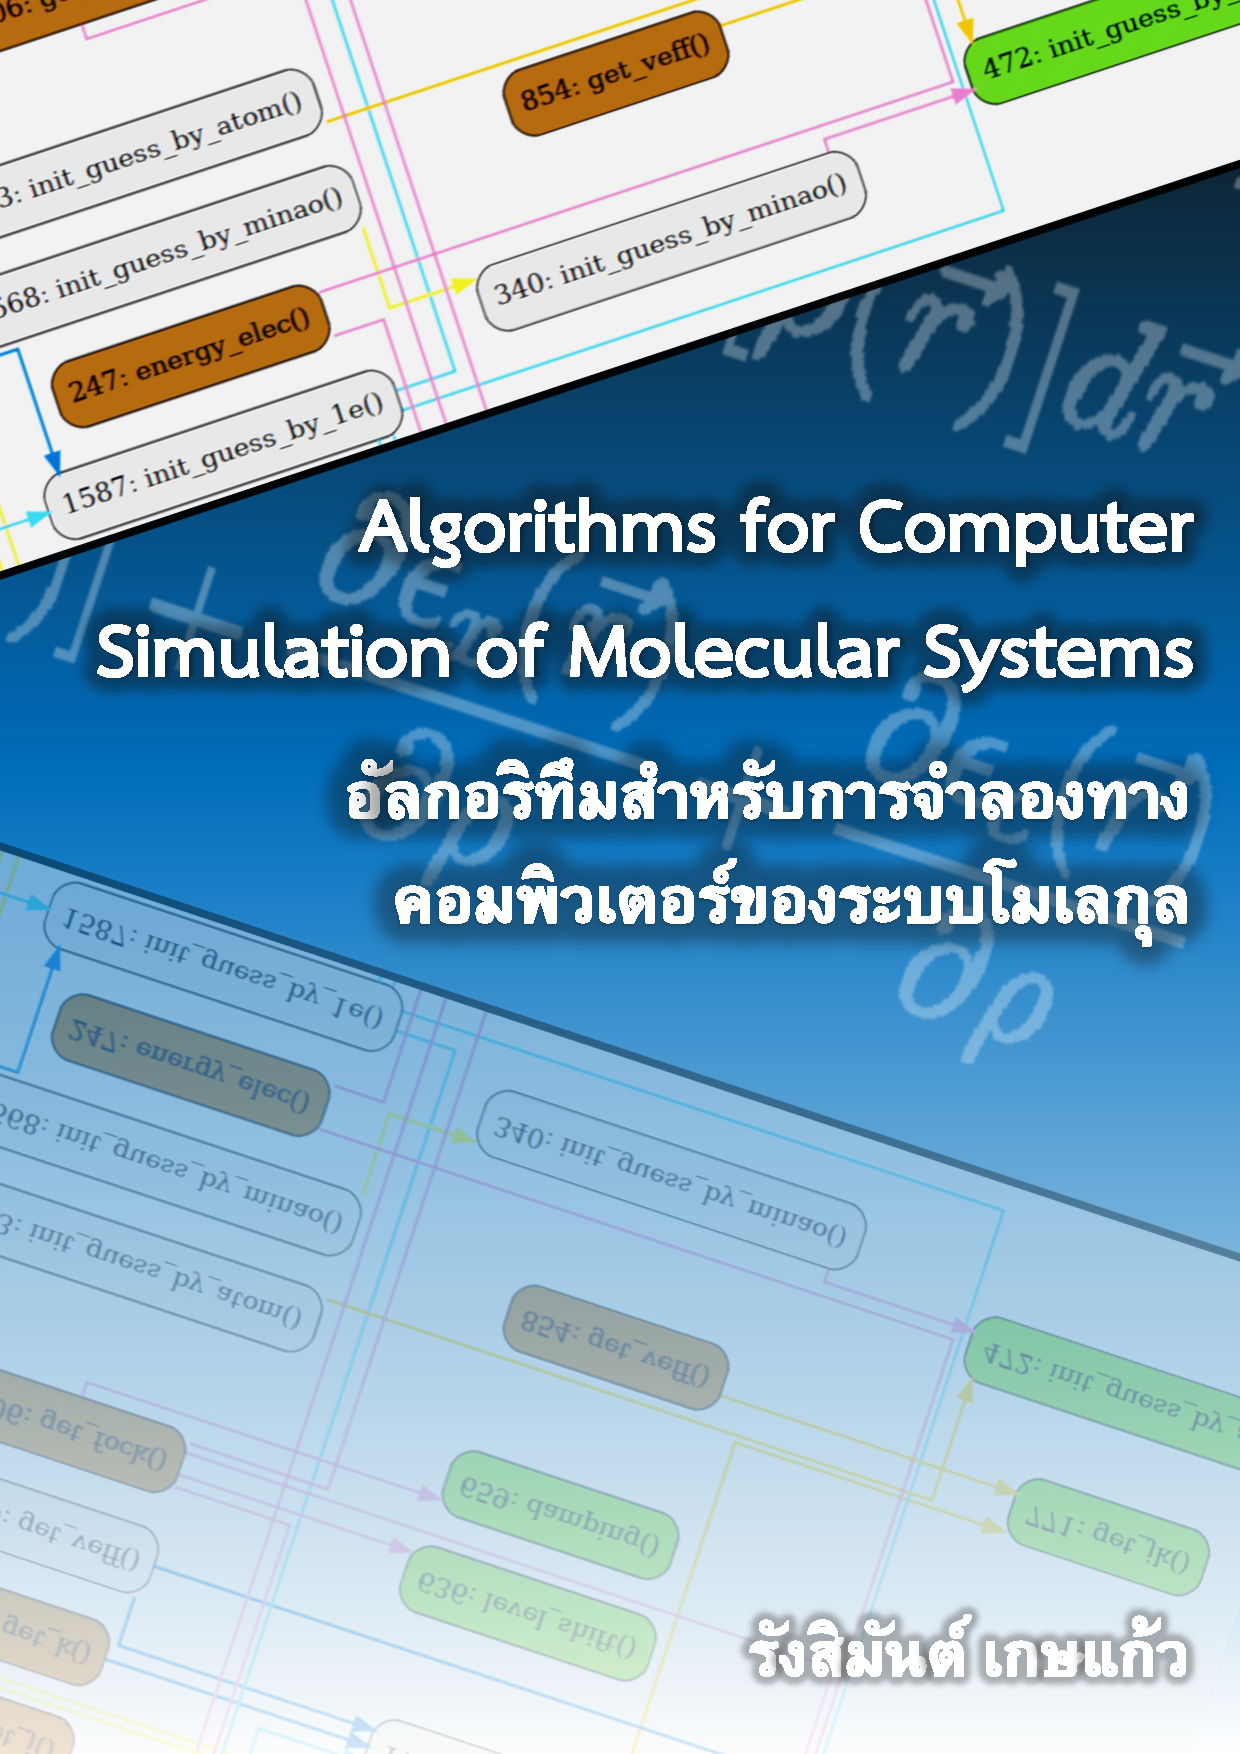
\includepdf[pages=-]{cover/cover_front.pdf}

\newpage
% empty page
\pagenumbering{gobble}
\newpage

\frontmatter
% LaTeX source for ``Algorithms for Computer Simulation of Molecular Systems''
% Copyright (c) 2023 รังสิมันต์ เกษแก้ว (Rangsiman Ketkaew).

% License: Creative Commons Attribution-NonCommercial-NoDerivatives 4.0 International (CC BY-NC-ND 4.0)
% https://creativecommons.org/licenses/by-nc-nd/4.0/

{
\thispagestyle{empty}

\begin{center}
    \vspace*{1.0in}
    
    \begin{spacing}{3}
    {\Huge Algorithms for Computer Simulation of Molecular Systems}\\
    {\LARGE อัลกอริทึมสำหรับการจำลองทางคอมพิวเตอร์ของระบบโมเลกุล}
    \end{spacing}
    
    \vspace{1.0in}
    
    {\LARGE  รังสิมันต์ เกษแก้ว}
    
    % \date{}
    \vspace{1.5in}
    
    {\LARGE ฉบับพิมพ์ครั้งที่ 1}
    \vspace{0.5in}
    
    %\includegraphics[width=1in]{figs/logo.pdf}
    \vfill
\end{center}
}

% LaTeX source for ``Ab initio Moleculardynamics''
% Copyright (c) 2023 รังสิมันต์ เกษแก้ว (Rangsiman Ketkaew).

% License: Creative Commons Attribution-NonCommercial-NoDerivatives 4.0 International (CC BY-NC-ND 4.0)
% https://creativecommons.org/licenses/by-nc-nd/4.0/

{
~\vfill
\thispagestyle{empty}
\setlength{\parindent}{0em}

รังสิมันต์ เกษแก้ว

Ab initio Molecular Dynamics\\
พลวัตเชิงโมเลกุลแบบแอบ อินิชิโอ

\bigskip

\par{ฉบับพิมพ์ครั้งที่ 1 พ.ศ. 2566}

สงวนลิขสิทธิ์ตาม พ.ร.บ. ลิขสิทธิ์ พ.ศ. 2537/2540

อนุญาตให้ผู้อื่นเผยแพร่ผลงานชิ้นนี้ได้ ตราบใดที่ให้เครดิตแก่ผู้เขียนในฐานะผู้สร้างต้นฉบับและลิงก์กลับไปที่สัญญาอนุญาตของเจ้าของผลงาน 
ไม่อนุญาตให้นำไปใช้เพื่อการค้าและดัดแปลงแก้ไขไม่ว่าด้วยวิธีใด เว้นแต่จะได้รับอนุญาตเป็นลายลักษณ์อักษรจากผู้เขียน

หนังสือเล่มนี้อยู่ภายใต้ลิขสิทธิ์สัญญาอนุญาตแบบเปิด A Creative Commons Attribution-NonCommercial-NoDerivatives 4.0 
International (CC BY-NC-ND 4.0), https://creativecommons.org/licenses/by-nc-nd/4.0/.

% Use absolute path of the file

\includegraphics[scale=1.2]{front_matter/by-nc-nd.pdf}

\bigskip

ซอร์สโค้ดของหนังสือเล่มนี้ถูกเขียนขึ้นโดยใช้ภาษา {\fontfamily{lmr}\selectfont \LaTeX} เผยแพร่ที่ 
\url{https://github.com/rangsimanketkaew/aimd-book} และไฟล์ PDF ถูกสร้างขึ้นโดยใช้ {\fontfamily{lmr}\selectfont 
\XeLaTeX} เผยแพร่ที่ \url{https://rangsimanketkaew.github.io/aimd-book}

หากต้องการติดต่อผู้เขียน กรุณาส่งอีเมลมาที่ rangsiman1993[at]gmail[dot]com
}

% LaTeX source for ``Algorithms for Computer Simulation of Molecular Systems''
% Copyright (c) 2023 รังสิมันต์ เกษแก้ว (Rangsiman Ketkaew).

% License: Creative Commons Attribution-NonCommercial-NoDerivatives 4.0 International (CC BY-NC-ND 4.0)
% https://creativecommons.org/licenses/by-nc-nd/4.0/

{
\pagestyle{empty} % make sure that no header on TOC pages
\tableofcontents
% \listoffigures
% \listoftables
}

% LaTeX source for ``Algorithms for Computer Simulation of Molecular Systems''
% Copyright (c) 2023 รังสิมันต์ เกษแก้ว (Rangsiman Ketkaew).

% License: Creative Commons Attribution-NonCommercial-NoDerivatives 4.0 International (CC BY-NC-ND 4.0)
% https://creativecommons.org/licenses/by-nc-nd/4.0/

{
% \pagenumbering{gobble}

\chapter*{\centering คำนำ}
\addcontentsline{toc}{chapter}{คำนำ}

การจำลองและคำนวณระบบโมเลกุลด้วยวิธีทางคอมพิวเตอร์นั้นช่วยให้นักวิทยาศาสตร์สามารถเข้าใจผลการทดลองในห้องปฏิบัติการ วิธีคำนวณทางเคมี%
ในระดับอะตอมนั้นสามารถแบ่งออกเป็นสองประเภทคือการคำนวณด้วยวิธีควอนตัม (Quantum Chemistry) และการคำนวณด้วยพลวัตเชิงโมเลกุล 
(Molecular Dynamics) ซึ่งทั้งสองวิธีนี้มีความแตกต่างกันอย่างสิ้นเชิงทั้งในแง่ทฤษฎี การใช้งานและความถูกต้องของการคำนวณ โดยวิธี Quantum 
Chemistry นั้นถูกนำมาใช้ในการศึกษาคุณสมบัติของโมเลกุลที่อธิบายด้วยโครงสร้างเชิงอิเล็กทรอนิกส์ซึ่งจะเกี่ยวข้องกับการคำนวณอันตรกิริยาระหว่าง%
อิเล็กตรอนโดยวิธีการประมาณ ในขณะที่วิธี Molecular Dynamics นั้นถูกนำมาใช้ศึกษาระบบโมเลกุลที่มีขนาดใหญ่และมีความซับซ้อนมากกว่าระบบ%
ที่โมเลกุลมีขนาดเล็กด้วยการจำลองการเคลื่อนที่ของอะตอมโดยอ้างอิงหลักกลศาสตร์แบบดั้งเดิม ซึ่งวิธีการนี้ช่วยให้เราศึกษาคุณสมบัติของโมเลกุลได้%
ในระดับของขนาดที่ใหญ่ขึ้นและระดับของระยะเวลาที่กว้างขึ้นด้วย

การจำลองทางคอมพิวเตอร์เพื่อศึกษาระบบโมเลกุลด้วยวิธี Molecular Dynamics แบบดั้งเดิมนั้นจะใช้แนวคิดของสนามแรง (Force Field) ซึ่งเป็น%
รูปแบบของฟังก์ชันทางคณิตศาสตร์ที่มีพารามิเตอร์ที่สามารถอธิบายพลังงานศักย์ของโมเลกุล (กลุ่มอะตอม) ซึ่งพลังงานศักย์ที่ได้มาจากการคำนวณ Force 
Field นี้คือสิ่งสำคัญที่เรามานำใช้ในการคำนวณแรงของอะตอมแต่ละอะตอมเพื่อใช้ในการหาโครงสร้างของโมเลกุล ณ จุดเวลาต่อ ๆ ไปได้ ซึ่งวิธี 
Molecular Dynamics แบบที่อ้างอิงกับ Force Field นั้นถูกนำมาใช้อย่างแพร่หลายในการศึกษาระบบต่าง ๆ เช่น การเปลี่ยนสถานะของสสาร 
ปฏิกิริยาเคมีหรือการเปลี่ยนแปลงเชิงโครงสร้างของชีวโมเลกุล นอกจากนี้การพัฒนา Force Field ก็เป็นหนึ่งในหัวข้องานวิจัยที่ได้รับความสนใจมาจน%
ถึงปัจจุบัน

แนวคิดของการรวมวิธีการคำนวณ Quantum Chemistry เข้ากับ Molecular Dynamics เพื่อเพิ่มความถูกต้องให้กับการคำนวณโดยการรวมนำข้อดี%
ของทั้งสองวิธีมารวมกันนั้นมีมานานมากกว่า 40 ปีแล้ว โดยวิธีการคำนวณที่ถูกพัฒนาขึ้นมาใหม่นี้มีชื่อเรียกว่า \textit{ab initio} Molecular 
Dynamics (AIMD) หรือพลวัตเชิงโมเลกุลแบบแอบ อินิชิโอ โดยในปัจจุบันวิธี AIMD นั้นมีความสำคัญและได้ถูกนำมาใช้อย่างแพร่หลายอย่างมากใน%
การจำลองระบบโมเลกุล โดยเฉพาะทางด้านวัสดุศาสตร์และฟิสิกส์ เช่น โครงสร้างผลึกและสภาวะของแข็งของโมเลกุล เพื่อศึกษาคุณสมบัติต่าง ๆ 
ของระบบเหล่านั้นก่อนที่จะมีการนำไปศึกษาจริงในห้องปฏิบัติการ ช่วยให้ประหยัดงบประมาณในการทำงานวิจัยได้อย่างมหาศาลและช่วยให้นักวิทยาศาสตร์%
เข้าใจถึงพฤติกรรมและอธิบายถึงปัจจัยที่ส่งผลต่อคุณสมบัติของโมเลกุลได้ด้วย 

เนื่องจากว่าในปัจจุบันนั้นแหล่งความรู้สำหรับการศึกษาอัลกอริทึมการจำลองทางคอมพิวเตอร์ของระบบโมเลกุลนั้นมักจะอยู่ในรูปของบทความวิชาการเป็น%
ส่วนใหญ่ ซึ่งบทความวิชาการเหล่านั้นส่วนใหญ่แล้วจะมีเนื้อหาที่ซับซ้อนและอาจจะทำให้ยากต่อการทำความเข้าใจของผู้ที่เพิ่มเริ่มศึกษา ยิ่งไปกว่านั้นผู้เขียน%
พบว่ายังไม่มีหนังสือหรือตำราทางวิชาการภาษาไทยที่เกี่ยวกับการจำลองทางคอมพิวเตอร์ของระบบโมเลกุล ดังนั้นหนังสือเล่มนี้จึงเป็นอีกช่องทางหนึ่งสำหรับ%
ผู้ที่สนใจและต้องการศึกษาอัลกอริทึมของ Molecular Dynamics เพื่อนำไปใช้ต่อยอดในงานวิจัยทางด้านเคมีทฤษฎีและเคมีเชิงคำนวณ รวมไปถึงสาขา%
ที่เกี่ยวข้องด้วย

สุดท้ายนี้ผู้เขียนหวังเป็นอย่างยิ่งว่าหนังสือเล่มนี้จะช่วยให้ผู้อ่านได้รับความรู้ที่ถูกต้องและครบถ้วนเกี่ยวกับวิธี AIMD ถ้าหากผู้อ่านมีข้อเสนอแนะ ข้อสงสัย%
หรือพบข้อผิดพลาดเกี่ยวกับเนื้อหาในหนังสือเล่มนี้สามารถติดต่อผู้เขียนได้โดยตรงผ่านทางอีเมล rangsiman1993[at]gmail[dot]com

\medskip

\begin{flushright}
รังสิมันต์ เกษแก้ว \\
12 มกราคม พ.ศ. 2566
\end{flushright}
}

% LaTeX source for ``Algorithms for Computer Simulation of Molecular Systems''
% Copyright (c) 2022 รังสิมันต์ เกษแก้ว (Rangsiman Ketkaew).

% License: Creative Commons Attribution-NonCommercial-NoDerivatives 4.0 International (CC BY-NC-ND 4.0)
% https://creativecommons.org/licenses/by-nc-nd/4.0/

{
% \pagenumbering{gobble}

\chapter*{\centering กิตติกรรมประกาศ}
\addcontentsline{toc}{chapter}{กิตติกรรมประกาศ}

ความรู้และแรงบัลดาลใจในการเขียนหนังสือเล่มนี้ของผู้เขียนมาจากแรงผลักดันและการสนับสนุนของบุคคลหลายท่าน 
การเขียนหนังสือเล่มนี้จะไม่เกิดขึ้นหรือสำเร็จไม่ได้ถ้าหากขาดบุคคลดังต่อไปนี้

ครอบครัวของผู้เขียนที่สนับสนุนให้ผู้เขียนได้ทำตามความฝันในการเรียนต่อระดับอุดมศึกษา ทั้งในระดับปริญญาโทและปริญญาเอก 
โดยเฉพาะการเห็นคุณค่าของการเรียนและการทำงานวิจัยทางด้านวิทยาศาสตร์พื้นฐาน

รศ.ดร. ยุทธนา ตันติรุ่งโรจน์ชัย บุคคลผู้เป็นต้นแบบด้านการเรียนและเป็นผู้สร้างแรงบันดาลใจให้ผู้เขียนเรียนต่อต่างประเทศและทำงานวิจัยทางด้าน%
เคมีทฤษฎีและเคมีคอมพิวเตอร์

อาจารย์และเพื่อน ๆ ในช่วงมัธยมศึกษา (ตอนต้น-ปลาย) ที่โรงเรียนพนัสพิทยาคาร และช่วงปริญญาตรี-โท ที่มหาวิทยาลัยธรรมศาสตร์ 
สำหรับความทรงจำอันดีงามและความเป็นกัลยาณมิตรที่ดีเสมอมา

เพื่อน ๆ ที่เมืองซูริค ประเทศสวิตเซอร์แลนด์ สำหรับมิตรภาพอันดีงาม รอยยิ้มและเสียงหัวเราะที่เกิดขึ้น รวมไปถึงกิจกรรมที่ได้ทำร่วมกันในระหว่าง%
ที่ผู้เขียนกำลังศึกษาปริญญาเอกซึ่งเป็นช่วงเวลาเดียวกันกับที่ผู้เขียนกำลังเขียนหนังสือเล่มนี้

เพื่อนร่วมงานทั้งนักศึกษาปริญญาโท ปริญญาเอก และนักวิจัยหลังปริญญาเอกของกลุ่มวิจัยของผู้เขียนที่ภาควิชาเคมี
มหาวิทยาลัยแห่งซูริค สำหรับการแลกเปลี่ยนความรู้ ไอเดียใหม่ ๆ และการช่วยเหลือเกี่ยวกับงานวิจัยทางด้านเคมีทฤษฎี

\medskip

\begin{flushright}
รังสิมันต์ เกษแก้ว
\end{flushright}
}

% LaTeX source for ``Algorithms for Computer Simulation of Molecular Systems''
% Copyright (c) 2023 รังสิมันต์ เกษแก้ว (Rangsiman Ketkaew).

% License: Creative Commons Attribution-NonCommercial-NoDerivatives 4.0 International (CC BY-NC-ND 4.0)
% https://creativecommons.org/licenses/by-nc-nd/4.0/

{
% \pagenumbering{gobble}

\chapter*{\centering สิ่งที่ควรทราบเกี่ยวกับหนังสือเล่มนี้}
\addcontentsline{toc}{chapter}{สิ่งที่ควรทราบเกี่ยวกับหนังสือเล่มนี้}

หนังสือเล่มนี้มีหนังสือต่างประเทศหลายเล่มเป็นแหล่งข้อมูลอ้างอิงทางวิชาการเพื่อให้มั่นใจได้ว่าความรู้ที่ผู้อ่านจะได้ศึกษาจากหนังสือเล่มนี้นั้นถูกต้อง อย่างไรก็ตามผมไม่สามารถการันตีได้ 100 เปอร์เซ็นต์ว่าหนังสือเล่มนี้ไม่มีข้อผิดพลาดเลยแม้แต่จุดเดียว ข้อผิดพลาดเล็กน้อยอาจจะเกิดจากการพิมพ์ผิด เป็นต้น ส่วนข้อผิดพลาดทางเนื้อหานั้นผมค่อนข้างมั่นใจว่ามีน้อยมากเพราะว่าผมได้ใช้หนังสือได้ที่รับการยอมรับและความนิยมในกลุ่มนักวิจัยทางด้าน Quantum Chemistry, Electronic Structure และ \textit{ab initio} Molecular Dynamics หลาย ๆ เล่มมาเป็นหนังสืออ้างอิง รวมถึงได้พูดคุยและสอบถามกับนักวิจัยด้านเคมีควอนตัมคนอื่น ๆ ทั้งที่เป็นเพื่อนรวมงานและคนที่ผมได้ไปพบเจอตามงานประชุมวิชาการ จึงทำให้มั่นใจได้ว่าความรู้ที่ถ่ายทอดผ่านหนังสือเล่มนี้นั้นถูกต้อง สำหรับสไตล์การใช้ภาษาในการเขียนหนังสือเล่มนี้ไม่วิชาการมากเกินไป ซึ่งผมพยายามเลือกใช้คำง่าย ๆ ให้มากที่สุด แต่ถึงอย่างนั้นก็ตามผมก็ไม่อาจที่จะหลีกเลี่ยงการใช้คำศัพท์เชิงเทคนิคได้

หนังสือ 6 เล่มที่ผมคิดว่าเขียนได้ดีมาก ๆ และผมใช้เป็นหนังสืออ้างอิงไม่เพียงแค่สำหรับเขียนหนังสือเล่มนี้แต่ยังใช้ในการทำงานวิจัยของผมเองด้วยมีดังนี้

\begin{figure}[H]
    \begin{center}
        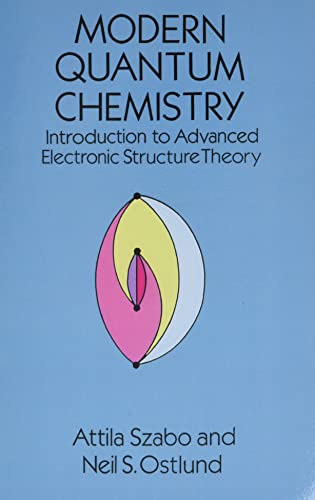
\includegraphics[height=5cm]{fig/modern-qm.jpg} 
        \hspace{0.5em}
        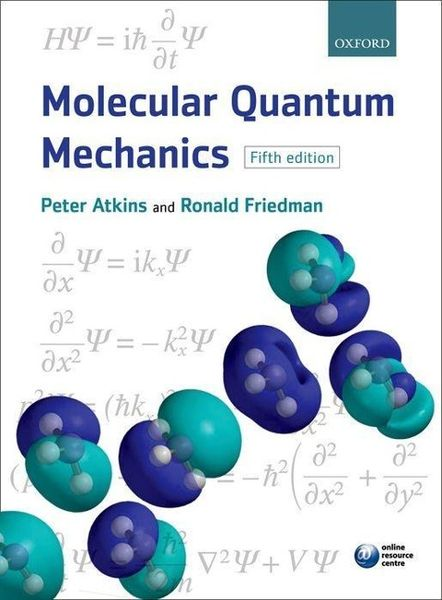
\includegraphics[height=5cm]{fig/mol-quan-mech.jpeg} 
        \hspace{0.5em}
        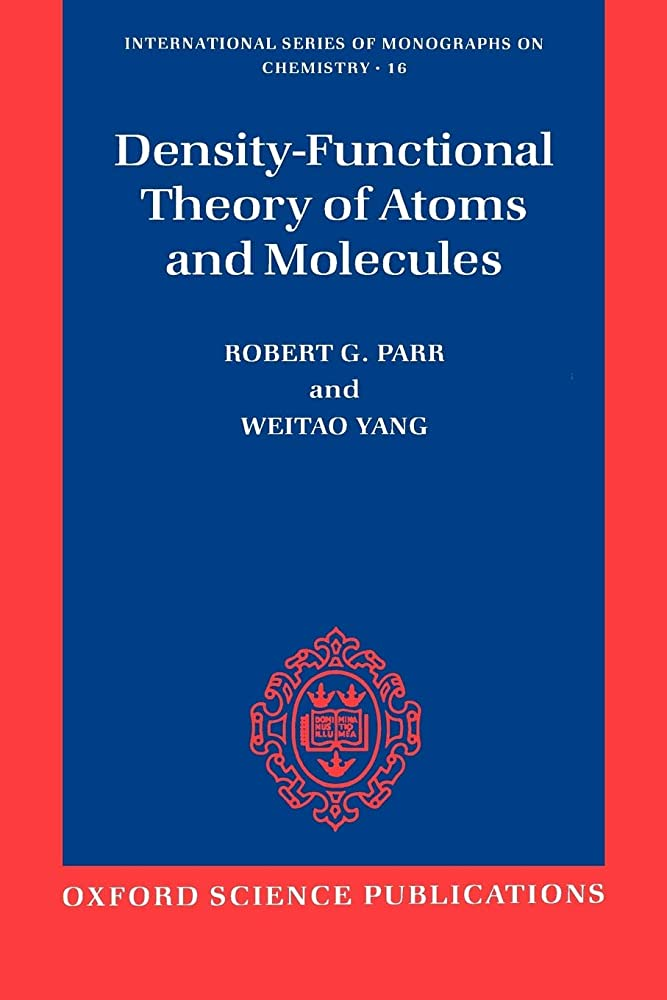
\includegraphics[height=5cm]{fig/dft-atom-mol.jpg} \\
        \vspace{1em}
        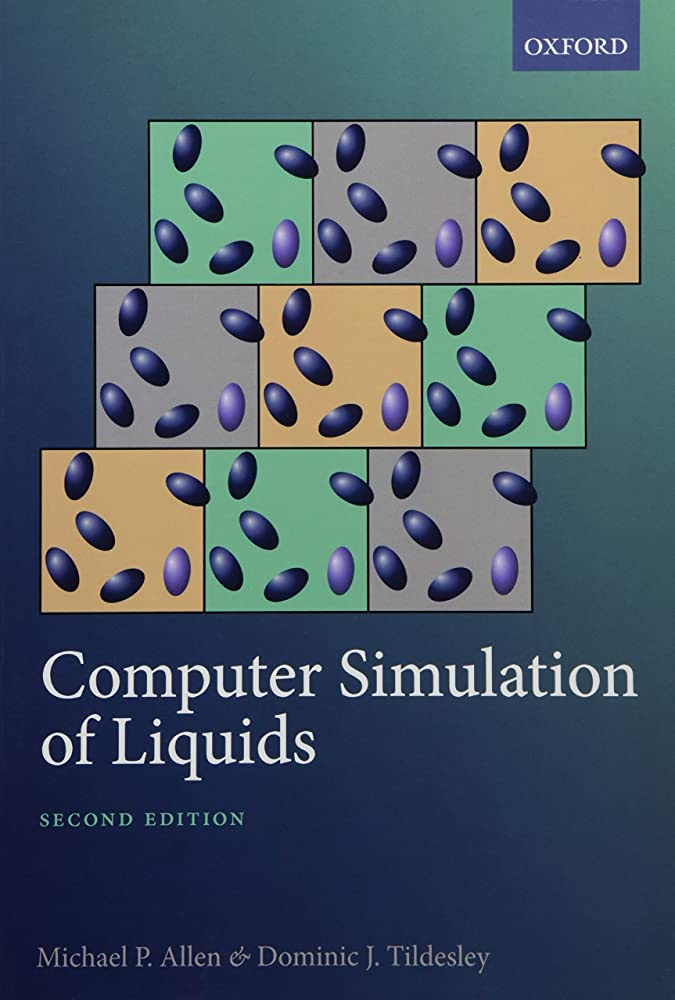
\includegraphics[height=5cm]{fig/com-sim-liq.jpg} 
        \hspace{0.5em}
        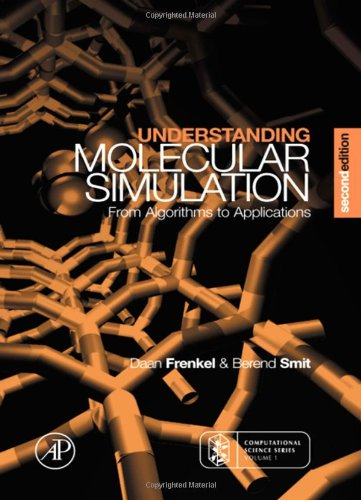
\includegraphics[height=5cm]{fig/understand-mol-sim.jpg}
        \hspace{0.5em}
        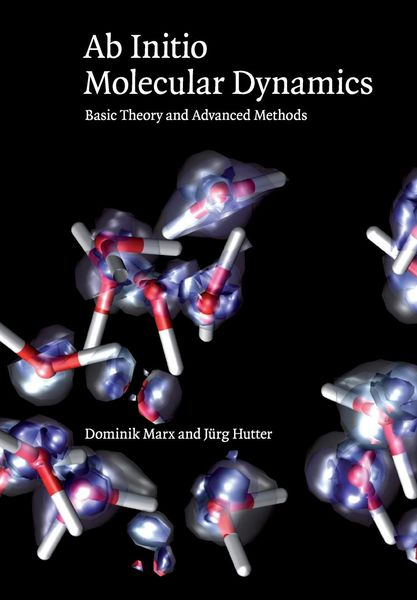
\includegraphics[height=5cm]{fig/aimd.jpeg}
    \end{center}
\end{figure}

\begin{enumerate}[topsep=0pt,noitemsep]
    \setlength\itemsep{0.5em}
    \item Modern Quantum Chemistry: Introduction to Advanced Electronic Structure Theory
    แต่งโดย Attila Szabo และ Neil S. Ostlund\autocite{szabo1996}

    \item Molecular Quantum Mechanics (5th Edition)
    แต่งโดย Peter W. Atkins และ Ronald S. Friedman\autocite{atkins2010}

    \item Density-Functional Theory of Atoms and Molecules 
    แต่งโดย Robert G. Parr และ Yang Weitao\autocite{parr1994}

    \item Computer Simulation of Liquids (2nd Edition)
    แต่งโดย Michael P. Allen และ Dominic J. Tildesley\autocite{allen2017}
    
    \item Understanding Molecular Simulation: From Algorithms to Applications (2nd Edition)
    แต่งโดย Daan Frenkel และ Berend Smit\autocite{frenkel2001}

    \item \textit{Ab Initio} Molecular Dynamics: Basic Theory and Advanced Methods
    แต่งโดย Dominik Marx และ Juerg Hutter\autocite{marx2009}
    
\end{enumerate}

หนังสือเล่มนี้\underline{เหมาะ}สำหรับนักศึกษา นักวิจัย ผู้ที่สนใจในสาขาเคมีทฤษฎีและเคมีคำนวณและผ่านการเรียนวิชาเคมีเชิงฟิสิกส์มาแล้ว โดยเนื้อหาในหนังสือเล่มนี้เน้นไปที่การอธิบายทฤษฎีและพิสูจน์ที่มาของสมการทางกลศาสตร์ควอนตัมและโครงสร้างเชิงอิเล็กทรอนิกส์ของอะตอมและโมเลกุลรวมถึงแบบจำลองของระบบโมเลกุล นอกจากนี้ยังอธิบายการประยุกต์ใช้อัลกอริทึมทางคอมพิวเตอร์สำหรับการเขียนโปรแกรมคำนวณและการประมวลผลบนคอมพิวเตอร์สมรรถนะสูงอีกด้วย

หนังสือเล่มนี้\underline{ไม่เหมาะ}สำหรับผู้ที่ยังไม่เคยเรียนวิชาเคมีเชิงฟิสิกส์หรือเคมีควอนตัมมาก่อนเพราะว่าอาจจะตกใจกับคำศัพท์ทางเทคนิคและสมการต่าง ๆ ได้ อย่างไรก็ตามถ้าหากผู้อ่านสามารถทำความเข้าใจเนื้อหาของหนังสือเล่มนี้ได้โดยที่ยังไม่เคยศึกษาเคมีควอนตัมมาก่อนเลยก็ถือว่าเยี่ยมมาก ๆ นอกจากนี้แล้วในการทำความเข้าใจเนื้อหาในหนังสือเล่มนี้นั้นจะต้องอาศัยความรู้ทางคณิตศาสตร์พีชคณิตเยอะมาก ๆ โดยเฉพาะความรู้เกี่ยวกับเวกเตอร์ เมทริกซ์ แคลคูลัส รวมไปถึงเทคนิคต่าง ๆ ทางคณิตศาสตร์ เช่น Optimization, Decomposition, และ Diagonalization ดังนั้นผู้อ่านควรจะต้องมีความรู้คณิคศาสตร์เหล่านี้มาบ้างแล้ว

คำแนะนำในการศึกษาทฤษฎีทางเคมีควอนตัมจากประสบการณ์ส่วนตัวของผมที่อยากจะแบ่งปันมี 3 ข้อคือ 

\begin{enumerate}[topsep=0pt,noitemsep]
    \setlength\itemsep{0.5em}
    \item \textbf{อ่านตำรา (Textbook) ทีละเล่ม} สำหรับผู้ที่เริ่มต้นนั้นควรเลือกหนังสือเพียงเล่มเดียว ถ้าหากว่าอ่านหลายเล่มพร้อม ๆ กันแล้วสลับอ่านไปมาก็อาจจะทำให้เกิดความสับสนได้เพราะว่าหนังสือแต่ละเล่มนั้นจะมีการใช้สัญลักษณ์หรือคำศัพท์เฉพาะทางที่ต่างกันได้
    
    \item \textbf{อ่านบทความวิชาการเพื่ออัพเดทความรู้} ปฏิเสธไม่ได้เลยว่าการทำวิจัยในปัจจุบันนั้นดำเนินไปอย่างรวดเร็วมาก ๆ เนื่องจากว่าเรามีคอมพิวเตอร์ที่มีประสิทธิภาพมากขึ้น รวมถึงกระบวนการตีพิมพ์งานวิชาการนั้นก็ไม่ได้ช้าเหมือนในอดีต ดังนั้นการอ่านบทความวิชาการ เช่น บทความวิจัย, บทความรีวิว รวมถึงสรุปข่าวต่าง ๆ จึงมีความสำคัญอย่างมากเพราะว่าเราจะได้อัพเดทความรู้ของเราตลอดเวลา

    \item \textbf{ฝึกเขียนโปรแกรม} การเขียนโปรแกรมนั้นจะมีลำดับขั้นตอนที่ชัดเจน ตรงไปตรงมา และไม่สามารถข้ามขั้นตอนได้ ถ้าหากว่าเราศึกษาการเขียนโปรแกรมควบคู่ไปกับการทฤษฎีที่สนใจก็จะทำให้เราเข้าใจที่มาที่ไปได้ง่ายขึ้น
\end{enumerate}

}

% LaTeX source for ``การเรียนรู้ของเครื่องสำหรับเคมีควอนตัม (Machine Learning for Quantum Chemistry)''
% Copyright (c) 2022 รังสิมันต์ เกษแก้ว (Rangsiman Ketkaew).

% License: Creative Commons Attribution-NonCommercial-NoDerivatives 4.0 International (CC BY-NC-ND 4.0)
% https://creativecommons.org/licenses/by-nc-nd/4.0/

{
\thispagestyle{empty}
~\vfill

\begin{doublespace}
\noindent\fontsize{16}{22}\selectfont\itshape
\nohyphenation
\vspace*{-0.8em}%
Erwin with his $\psi$ can do\\
\vspace*{-0.8em}%
Calculations quite a few.\\
\vspace*{-0.8em}%
But one thing has not been seen,\\
Just what does $\psi$ really mean.\\
\noindent - \mbox{Walter H\"{u}ckel} (1895 - 1973)
\end{doublespace}

\vfill
\vfill
}


\pagestyle{fancy} % Add header from this page on

\mainmatter

% LaTeX source for ``Algorithms for Computer Simulation of Molecular Systems''
% Copyright (c) 2023 รังสิมันต์ เกษแก้ว (Rangsiman Ketkaew).

% License: Creative Commons Attribution-NonCommercial-NoDerivatives 4.0 International (CC BY-NC-ND 4.0)
% https://creativecommons.org/licenses/by-nc-nd/4.0/

\chapter{กลศาสตร์ควอนตัมเชิงโมเลกุล}
\label{ch:mol_qm}

%----------------------------------------
\section{การจำลองเชิงตัวเลขและเทคนิคเชิงคอมพิวเตอร์}
%----------------------------------------

การจำลองเชิงตัวเลข (Numerical Modeling) คือวิธีที่การที่เราใช้ปัญหาทางคณิตศาสตร์และฟิสิกส์แบบต่าง ๆ เช่น นำมาใช้แก้สมการเชิง%
อนุพันธ์ที่ใช้ในการอธิบายปรากฏการณ์ต่าง ๆ ทางธรรมชาติซึ่งอาจจะมีความยากหรืออาจจะไม่มีทางแก้ได้ด้วยวิธีเชิงวิเคราะห์ (Analytical Method)
\idxboth{การจำลองเชิงตัวเลข}{Numerical Modeling}
\idxboth{วิธีเชิงวิเคราะห์}{Analytical Method}

สำหรับการจำลองด้วยเทคนิคเชิงคอมพิวเตอร์ (Computer Simulation) นั้นเป็นการศึกษาการตอบสนองเชิงพลวัต (Dynamic Response) 
ของระบบแบบจำลองต่อเงื่อนไขเริ่มต้น (Initial Conditions) ที่เราได้กำหนดไว้ โดยเงื่อนไขเริ่มต้นนี้สอดคล้องกับสภาวะจริงของระบบนั้น
\idxboth{เทคนิคเชิงคอมพิวเตอร์}{Computer Simulation}
\idxboth{เงื่อนไขเริ่มต้น}{Initial Conditions}

\begin{figure}[htbp]
    \centering
    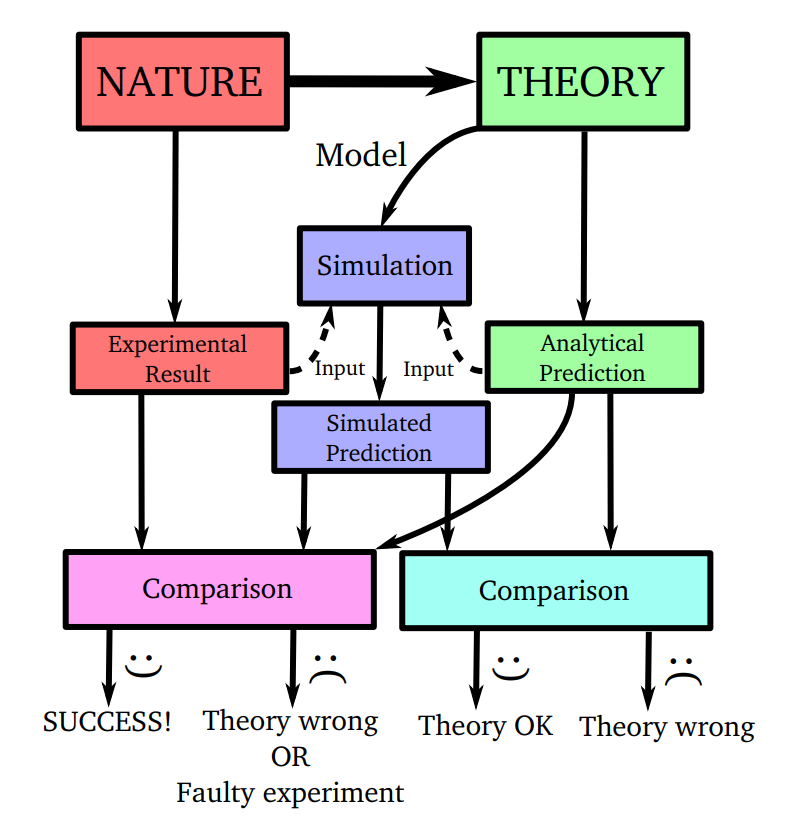
\includegraphics[width=0.8\linewidth]{fig/simulation-modeling-graph.png}
    \caption{แผนผังความเชื่อมโยงของระบบที่เราต้องศึกษา (Nature), ทฤษฎีหรือวิธีที่ใช้ในการศึกษา (Theory), แบบจำลองหรือโมเดล 
    (Model), ผลการทดลอง (Experimental Result), และผลการคำนวณหรือผลการทำนาย (Computational Results หรือ Prediction)}
    \label{fig:sim_model_graph}
\end{figure}

ภาพที่ \ref{fig:sim_model_graph} แสดงแผนผังเชื่อมโยงความแตกต่างระหว่าง Numerical Modeling กับ Computer Simulation 
นั้นก็คือใน Simulation นั้นระบบจำลองของเราจะถูกสร้างขึ้นมา เช่น เราสร้างระบบที่เป็นโมเลกุลน้ำหลาย ๆ โมเลกุลเกาะกลุ่มรวมกัน (Water 
Cluster) โดยเราหวังว่า Water Cluster ที่เราสร้างขึ้นมานี้จะสามารถเป็นตัวแทนของระบบของโมเลกุลน้ำจริง ๆ ได้ ซึ่งก็จะทำให้เราสามารถ%
ศึกษาคุณสมบัติต่าง ๆ ของโมเลกุลน้ำได้ตามต้องการ ส่วนการจำลองเชิงตัวหรือ Numerical Simulation นั้นจะเป็นการสร้างการทดลองเสมือนจริง 
(Virtual Experiments) ของระบบจำลองขึ้นมา อย่างไรก็ตามในบทความวิชาการทางด้านเคมีเชิงคำนวณหรือชีวเชิงคำนวณนั้นเรามักจะพบว่าคำว่า 
Modeling นั้นสามารถถูกแทนด้วยคำว่า Simulation ได้เช่นกัน

คำถามสำคัญที่หลายคนโดยเฉพาะอย่างนักวิทยาศาสตร์ที่ทำงานวิจัยเชิงการทดลองมักจะถามก็คือ \enquote{ทำไมการจำลองทางคอมพิวเตอร์ถึง%
มีความสำคัญ} ซึ่งคำตอบนั้นมีด้วยกันหลายข้อโดยผมขอสรุปเป็นประเด็นตามนี้ครับ

\begin{enumerate}
    \item การจำลองทางคอมพิวเตอร์นั้นเปรียบเสมือนเป็นสะพานเชื่อมโยงระหว่างทฤษฎีกับการทดลอง
    
    \item การทำการทดลองบางอย่างนั้นมีค่าใช้จ่ายที่สูงมากและมีความยากเพราะว่าตัวทฤษฎีนั้นซับซ้อนเกินไป ดังนั้นการจำลองทางคอมพิวเตอร์%
    นั้นจะเข้ามาช่วยในการจำลองการทดลองและทดสอบสมมติฐานเพื่อยืนยันทฤษฎีด้วย
    
    \item การจำลองทางคอมพิวเตอร์นั้นช่วยหาปัจจัยและเงื่อนไขที่เหมาะสมสำหรับการทดลองได้
    
    \item การจำลองทางคอมพิวเตอร์สามารถแสดงกระบวนการของระบบที่เราสนใจได้ ซึ่งอาจจะทำได้ยากในเชิงการทดลอง
    
    \item การจำลองทางคอมพิวเตอร์สามารถนำมาใช้ในการศึกษาปรากฏการณ์ที่การทดลองนั้นอาจจะให้ผลการทดลองที่ไม่ละเอียดพอ
\end{enumerate}

อย่างไรก็ตามผมต้องขอสรุปเพิ่มเติมด้วยว่าการใช้แบบจำลองทางคอมพิวเตอร์เพียงอย่างเดียวนั้นจะเปล่าประโยชน์ถ้าหากว่าไม่มีผลการทดลองที่%
น่าเชื่อมายืนยันความถูกต้องของผลการคำนวณ ดังนั้นเคมีเชิงการทดลองกับเคมีเชิงคำนวณนั้นจึงเป็นศาสตร์ที่ต้องพึ่งพาอาศัยกัน

%----------------------------------------
\section{สมการชโรดิงเงอร์}
\idxboth{สมการชโรดิงเงอร์}{Schr\"{o}dinger Equation}
%----------------------------------------

สมการชโรดิงเงอร์เป็นสิ่งที่ช่วยให้เราสามารถเข้าใจพฤติกรรมของโมเลกุลได้ การที่เรารู้คำตอบหรือผลเฉลยของสมการนั้นนำไปสู่การเข้าใจข้อมูลต่าง ๆ
ของโมเลกุล (พูดให้ครอบคลุมกว่านี้คือระบบแบบ Microscopic) ที่อุณหภูมิ 0 K โดยสมการชโรดิงเงอร์ที่ขึ้นกับเวลา (Time-dependent 
Schr\"{o}dinger Equation) นั้นมีหน้าตาดังนี้

\begin{equation}
    \label{eq:time_dependent_schrodinger}
    \hat{\mathscr{H}} \Psi\left(\vec{r}_{1 \ldots N}, t\right) 
    = \mathrm{i} \hbar \frac{\partial \Psi\left(\vec{r}_{1 \ldots N}, t\right)}{\partial t}
\end{equation}

\noindent โดยที่ตัวแปรในสมการมีดังนี้
\begin{itemize}[topsep=0pt,noitemsep]
    \setlength\itemsep{1em}
    \item $\hat{\mathscr{H}}$ คือโอเปอร์เรเตอร์ของพลังงาน
    
    \item $\Psi$ คือฟังก์ชันคลื่นที่ขึ้นอยู่กับพิกัดหรือตำแหน่งของอนุภาค (ในที่นี้คืออิเล็กตรอน) ทั้งหมด $N$ ตัว เราจึงใช้เวกเตอร์แทน 
    $\vec{r}_{1}, \vec{r}_{2}, \dots, \vec{r}_{N}$ 
    
    \item $i$ คือหน่วยจินตภาพ $(\sqrt{-1})$
    
    \item $\hbar$ คือค่าคงที่ของพลังค์แบบลดรูป (Reduced Planck's constant) มีค่าเท่ากับ 
    \num{1.05457182e-34} \si{m^{2}.kg.s^{-1}}
\end{itemize}

ตัวแปรที่น่าจะมีความสำคัญที่สุดก็คือ $\hat{H}$ ซึ่งเป็นโอเปอร์เรเตอร์ที่ที่เป็นผลรวมของโอเปอร์เรเตอร์พลังงานศักย์และโอเปอร์เรเตอร์พลังงานจลน์ 
ดังนี้

\begin{equation}
    \label{eq:hamiltonian_operator}
    \hat{\mathscr{H}} = \hat{\mathscr{T}}+\hat{V}
\end{equation}

\noindent โดยที่โอเปอร์เรเตอร์พลังงานจลน์ของระบบ $\hat{\mathscr{T}}$ นั้นก็คือผลรวมของโอเปอร์เรเตอร์พลังงานจลน์ของอนุภาคแต่ละตัวนั่นเอง

\begin{equation}
    \label{eq:kinetic_operator}
    \hat{\mathscr{T}} = \sum_{i=1}^N \frac{-\hbar^2}{2 m_i} \nabla_i^2
\end{equation}

\noindent โดยที่ $m_i$ คือมวลของอนุภาค $i$, $N$ คือจำนวนของอนุภาค และ $\nabla_i^2$ คือ Laplacian ในพิกัดคาร์ทีเซียนของอนุภาค 
$i$ ซึ่งมีสมการดังนี้

\begin{equation}
    \label{eq:nabla}
    \nabla_i^2 
    = \frac{\partial^2}{\partial x_i^2} 
        + \frac{\partial^2}{\partial y_i^2} 
        + \frac{\partial^2}{\partial z_i^2}
\end{equation}

\noindent โดยที่ $\vec{r}_i = \left(x_i, y_i, z_i\right)$ คือเวกเตอร์ของตำแหน่งในพิกัดคาร์ทีเซียน 

ส่วนพลังงานจลน์ของระบบ ($\hat{V}\left(\vec{r}_{1 \ldots N}\right)$) นั้นจริง ๆ แล้วมีความซับซ้อนมากเพราะว่าประกอบไปด้วย%
พลังงานจลน์หลาย ๆ รูปแบบมารวมกันแล้วก็จะมีความเฉพาะต่อระบบที่เราศึกษา สำหรับเคมีนั้นระบบที่เราสนใจศึกษาคือโมเลกุลดังนั้นโอเปอร์เรเตอร์%
พลังงานศักย์นั้นจะต้องสอดคล้องกับพลังงานศักย์ของนิวเคลียสและอิเล็กตรอนเป็นหลักซึ่งผู้อ่านจะได้ศึกษาในหัวข้อที่ 

คราวนี้เรากลับมาดูที่ฟังก์ชันคลื่นกันต่อ ถ้าหากว่าฟังก์ชันคลื่นของเรานั้นเป็นฟังก์ชันที่ขึ้นอยู่กับตำแหน่งของอนุภาคเพียงอย่างเดียวและไม่ขึ้นกับเวลา 
เราสามารถเขียนฟังก์ชันคลื่นของทั้งระบบให้อยู่ในรูปผลคูณของฟังก์ชันคลื่นของอนุภาคแต่ละตัวได้โดยใช้เทคนิคที่เรียกว่า Separation of Variables 
ซึ่งเราจะได้สมการดังนี้

\begin{equation}
    \Psi\left(\vec{r}_{1 \ldots N}, t\right) = \psi\left(\vec{r}_{1 \ldots N}\right) \theta(t)
\end{equation}

\noindent ซึ่งเมื่อเรานำสมการด้านบนแทนเข้าไปในสมการชโรดิงเงอร์เราจะได้สมการดังนี้

\begin{equation}
    \frac{1}{\psi} \hat{H} \psi = \mathrm{i} \hbar \frac{1}{\theta} \frac{\partial \theta}{\partial t}
\end{equation}

เนื่องจากว่าฝั่งซ้ายของสมการนั้นเป็นฟังก์ชันที่ขึ้นกับ $\vec{r}_{1 . . . N}$ อย่างเดียวและฝั่งขวานั้นเป็นฟังก์ชันที่ขึ้นกับ $t$ ดังนั้นทั้งสองฝั่ง%
นั้นจะต้องมีค่าเท่ากับค่าคงที่ค่าหนึ่งซึ่งก็คือพลังานของระบบ $E$ แล้วเราจะได้ว่าสมการโชรดิงเงอร์ที่ขึ้นกับเวลานั้นจะเปลี่ยนเป็นสมการชโรดิงเงอร์ที่%
ไม่ขึ้นกับเวลา (Time-independent Schr\"{o}dinger Equation) ซึ่งมีสมการดังนี้

\begin{equation}
    \label{eq:time_independent_schrodinger}
    \hat{\mathscr{H}} \psi = E \psi
\end{equation}

สำหรับ Hamiltonians เกือบทั้งหมด (ไม่ใช้ทุกอัน) นั้นจะมีผลเฉลยสำหรับ Time-independent Schr\"{o}dinger Equation ที่มีค่าที่แน่นอน 
(Quantized) สำหรับแต่ละ State $n$ ของอนุภาค ดังนี้

\begin{equation}
    \hat{\mathscr{H}} \psi_n = E_n \psi_n
\end{equation}

\noindent ซึ่งเราสามารถตีความสมการด้านบนได้ว่าอนุภาคควอนตัมที่อยู่ในสถานะที่ $n$ จะมีค่าพลังงานที่แน่นอนนั้น $E_n$ นอกจากนี้แล้วสมการ%
ด้านบนนั้นเป็นปัญหาแบบค่าไอเกน (Eigenvalue Problem) โดยที่ $E_n$ คือค่าไอเกนและ $\psi_n$ คือฟังก์ชันไอเกนของโอเปอร์เรเตอร์ 
$\hat{\mathscr{H}}$ ซึ่งการที่เราจะแก้สมการ Time-independent Schr\"{o}dinger Equation นั้นจะต้องอาศัยเทคนิคพิเศษซึ่งจะได้ศึกษา%
ต่อในบทต่อ ๆ ไป\footnote{ตั้งแต่ส่วนนี้ของหนังสือเป็นต้นไปสมการโชรดิงเงอร์ (Schr\"{o}dinger Equation) นั้นจะหมายถึงสมการ%
ชโรดิงเงอร์แบบที่ไม่ขึ้นกับเวลา (Time-independent Schr\"{o}dinger Equation) ถ้าหากผมต้องการที่จะใช้คำว่าสมการชโรดิงเงอร์แบบ%
ที่ขึ้นกับเวลา (Time-dependent Schr\"{o}dinger Equation) ก็จะเขียนใช้คำนี้ตรง ๆ เลย}

%----------------------------------------
\section{แฮมิลโทเนียนเชิงโมเลกุล}
\idxboth{แฮมิลโทเนียนเชิงโมเลกุล}{Hamiltonian!Molecular Hamiltonian}
%----------------------------------------

ในวิชาเคมีควอนตัมนั้นเราจะนิยามว่าโมเลกุลนั้นประกอบไปด้วยอิเล็กตรอน $n$ ตัวและนิวเคลียส $N$ ตัว โดยมีคุณสมบัติดังต่อไปนี้

\begin{itemize}[topsep=0pt,noitemsep]
    \setlength\itemsep{1em}
    \item อิเล็กตรอนมีประจุเท่ากับ $-e$ 
    
    \item อิเล็กตรอนมีมวลเท่ากับ $m_e$ 
    
    \item นิวเคลียสตัวที่ $I$ นั้นมีประจุเท่ากับ $Z_I e$ 
    
    \item นิวเคลียสตัวที่ $I$ มีมวลเท่ากับ $m_I$ 
\end{itemize}

\noindent โดยที่อิเล็กตรอนกับนิวเคลียสนั้นจะถูกพิจารณาว่าเป็นจุดประจุ (Point Charges) 

โอเปอร์เรเตอร์พลังงานจลน์ $\hat{\mathscr{T}}$ สำหรับโมเลกุลนั้นเราสามารถประยุกต์ใช้สมการที่ \ref{eq:kinetic_operator} ได้ซึ่งก็%
คือพลังงานจลน์ของทั้งอิเล็กตรอนและนิวเคลียสรวมกัน ดังนี้

\begin{equation}
    \label{eq:kinetic_operator_molecule}
    \hat{\mathscr{T}} 
    = \underbrace{\sum_{I=1}^N \frac{-\hbar^2}{2 m_I} \nabla_I^2}_{\text{Nuclei}} 
        + \underbrace{\sum_{i=1}^n \frac{-\hbar^2}{2 m_e} \nabla_i^2}_{\text{Electrons}}
\end{equation}

ส่วนโอเปอร์เรเตอร์พลังงานศักย์ $\hat{V}$ สำหรับโมเลกุลนั้นก็จะเป็นอันตรกิริยาคูลอมบ์ (Coulomb Interaction) ระหว่างจุดประจุ ดังนี้

\begin{equation}
    \label{eq:potential_operator_molecule}
    \hat{\mathcal{V}} 
    = \underbrace{\sum_{\substack{I=1,1}}^N \frac{Z_I Z_J e^2}{4 \pi \varepsilon_0 R_{I J}}}
        _{\text{Nucleus-Nucleus}}
        + \underbrace{\sum_{i=1}^n \sum_{I=1}^N \frac{-Z_I e^2}{4 \pi \varepsilon_0 r_{i I}}}
            _{\text{Electron-Nucleus}}
        + \underbrace{\sum_{\substack{i=1,1 \\ j=i+1}}^n \frac{e^2}{4 \pi \varepsilon_0 r_{i j}}}
            _{\text{Electron-Electron}}
\end{equation}

\noindent ซึ่งก็คืออันตรกิริยาระหว่างทุกคู่ที่เป็นไปได้ นั่นคือ Nucleus-Nucleus, Electron-Nucleus และ Electron-Electron 
ส่วน $Z_I e$ นั้นก็คือประจุของนิวเคลียสที่ $I$ ซึ่ง $Z_I$ นั้นก็คือเลขอะตอมของนิวเคลียส เช่น ไฮโดรเจนนั้นก็จะมี $Z_I = 1$ และคาร์บอน%
ก็จะมี $Z_I=6$ ส่วน $e$ นั้นคือประจุของอิเล็กตรอนซึ่งก็คือ $-e$ นั่นเอง 

โดยปกติแล้วเรามักจะใช้ตัวห้อยที่เป็นอักษรภาษาอังกฤษตัวใหญ่ $I, J, K, \ldots$ เพื่อบ่งบอกถึงนิวเคลียสและใช้ตัวอักษรตัวเล็กสำหรับอิเล็กตรอน  
แล้วก็จะใช้ $R$ แทนระยะห่างที่วัดจากนิวเคลียสและใช้ $r$ แทนระยะห่างที่วัดจากอิเล็กตรอนอย่างน้อยหนึ่งตัว อย่างไรก็ตามในเคมีควอนตัมนั้นเรา%
มักจะใช้หน่วยของปริมาณต่าง ๆ ในหน่วยอะตอม (atomic units หรือ a.u.) แทนที่จะใช้หน่วย SI เพราะว่าสะดวกต่อการคำนวณโดยสามารถดู%
ได้ตามตาราง 

\begin{equation*}
    \begin{array}{|l|ll|}
        \hline \text{Charge of electron:} e=-1 & \text{Length:} & 1 \text{bohr} = \num{0.529177} \AA \\
        \text{Mass of electron:} m_e=1 & \text{Energy:} & 1 \text{hartree} = \num{2625.4996} \mathrm{~kJ} / \mathrm{mol} \\
        \hbar=h / 2 \pi=1 & & 1 \text{hartree} = \num{27.2113845} \mathrm{eV} \\
        4 \pi \varepsilon_0=1 & & \\
        \hline
    \end{array}
\end{equation*}

ถ้าเราเขียนโอเปอร์เรเตอร์พลังงานจลน์โดยใช้ atomic units จะได้ดังนี้

\begin{equation}
    \label{eq:kinetic_operator_au}
    \hat{\mathscr{T}} 
    = \underbrace{-\frac{1}{2} \sum_{I=1}^N \frac{1}{m_I} \nabla_I^2}_{\text{nuclei}} 
        - \underbrace{\frac{1}{2} \sum_{i=1}^n \nabla_i^2}_{\text{electrons}}
\end{equation}

\noindent และสำหรับโอเปอร์เรเตอร์พลังงานศักย์

\begin{equation}
    \label{eq:potential_operator_au}
    \hat{V} 
    = \underbrace{\sum_{\substack{I=1, J=I+1}}^N \frac{Z_I Z_J}{R_I}}_{\text{nucleus-nucleus}} 
        + \underbrace{\sum_{i=1}^n \sum_{I=1}^N \frac{-Z_I}{r_{i I}}}_{\text{electron-nucleus}} 
        + \underbrace{\sum_{\substack{i=1,1 \\ j=i+1}}^n \frac{1}{r_{i j}}}_{\text{electron-electron}}
\end{equation}

\noindent ซึ่งถ้าหากเราเขียน Hamiltonian ของโมเลกุล $\hat{\mathscr{H}}^{\mathrm{mol}}$ โดยรวมโอเปอร์เรเตอร์ทั้งสองตัวเข้าด้วยกัน 
จะได้ดังนี้

\begin{equation}
    \label{eq:hamiltonian_operator_molecule}
    \hat{\mathscr{H}}^{\mathrm{mol}} 
    = \hat{\mathscr{T}}_n 
        + \hat{\mathscr{T}}_e 
        + \hat{V}_{n n} 
        + \hat{V}_{e n} 
        + \hat{V}_{e e}
\end{equation}

\noindent โดยสองเทอมแรกนั้นก็คือพลังงานจลน์และสามเทอมที่เหลือนั้นก็คือพลังงานศักย์คูลอมบ์

%----------------------------------------
\section{คุณสมบัติพื้นฐานของฟังก์ชันคลื่น}
%----------------------------------------

โอเครครับ เราได้ศึกษาโอเปอร์เรเตอร์ Hamiltonian กันไปคร่าว ๆ แล้ว ในหัวข้อนี้เราจะมาดูรายละเอียดของฟังก์ชันคลื่นกันซึ่งผมจะขออธิบาย%
คุณสมบัติพื้นฐานของฟังก์ชันคลื่นก่อนซึ่งถือว่าเป็นพื้นฐานสำคัญมาก ๆ ที่ผู้อ่านควรจะต้องทราบและเข้าใจก่อนที่จะไปศึกษาฟังก์ชันคลื่นแบบเชิงลึกต่อ%
ไปในบทอื่น ๆ โดยคุณสมบัติของฟังก์ชันคลื่นที่ผมเลือกมาอธิบายนั้นจะเป็นคุณสมบัติที่สำคัญ ๆ เท่านั้นซึ่งจำเป็นและเพียงพ่อต่อการทำความเข้าใจ%
ในบทต่อ ๆ ไป

ก่อนอื่นเลยผมขออ้างการตีความฟังก์ชันคลื่นของบอนส์ (Born's Interpretation) ที่ว่า $\psi_i^* \psi_i \mathrm{~d} \tau$ 
นั้นคือความน่าจะเป็นสำหรับอนุภาคที่อยู่ในสภาวะ $i$ ในอนุภาคที่มีปริมาตรเล็กมาก ๆ ($\mathrm{d} \tau$) โดยที่ $\psi_i^*$ นั้นแทน%
คอนจูเกตเชิงซ้อน (Complex Conjugate) ของฟังก์ชันคลื่น $\psi_i$ นั่นหมายความว่าฟังก์ชันคลื่นอาจจะมีส่วนเชิงซ้อนเป็นองค์ประกอบก็ได้ 
อย่างไรก็ตามความน่าจะเป็น $\psi_i^* \psi_i \mathrm{~d} \tau$ มีเฉพาะส่วนจริงเป็นองค์ประกอบเท่านั้นซึ่งสอดคล้องกับเงื่อนไขที่ว่า%
จะต้องสามารถสังเกตได้ (Observable) 

กำหนดให้ความน่าจะเป็นสำหรับสถานะที่ $i$ ซึ่งเขียนแทนด้วย $\rho_i(\vec{r})$ นั้นถูกทำให้เป็นปกติ (ถูก Normalized แล้ว) เราจะตีความ%
ได้ว่าความน่าจะเป็นรวมที่จะพบอนุภาคที่ตำแหน่งไหนก็ตามใน Space นั้นจะมีค่าเท่ากับ 1 ซึ่งเขียนแทนด้วยสมการดังนี้

\begin{equation}
    \begin{aligned}
        \int_{\text{all space}} \rho_i \mathrm{~d} \tau 
        & = \int_{\text{all space}} \psi_i^* \psi_i \mathrm{~d} \tau \\
        & = 1
    \end{aligned}
\end{equation}

\noindent โดยที่ $\mathrm{d} \tau$ คือปริมาตรในพิกัดคาร์ทีเซียนสำหรับอนุภาคหนึ่งตัวซึ่งมีนิยามแบ่งตามพิกัดอ้างอิง ดังนี้

\begin{itemize}
    \item พิกัดคาร์ทีเซียน $\mathrm{d} \tau = \mathrm{d} x \mathrm{~d} y \mathrm{~d} z$ 
    
    \item พิกัดเชิงขั่วมีนิยามคือ $\mathrm{d} \tau = r^2 \sin (\theta) \mathrm{d} r \mathrm{~d} \theta \mathrm{d} \varphi$
\end{itemize}

\noindent ซึ่งถ้าหากเราทำอินทิเกรตทั่วทั้งปริมาตรเราสามารถละขอบเขตการอินทิเกรตออกไปได้ ดังนี้

\begin{equation}
    \int_{\text{all space}} \ldots \mathrm{d} \tau \equiv \int \ldots \mathrm{d} \tau
\end{equation}

นอกจากนี้เรายังพบว่าถ้า $\psi$ นั้นถูก Normalized แล้ว $\Psi(t)$ ก็จะถูก Normalized ด้วย ซึ่งเราก็จะได้ความสัมพันธ์ดังนี้ 

\begin{equation}
    \Psi^*(t) \Psi(t) = \psi^* \psi
\end{equation}

สำหรับนิยามถัดมาก็คือโอเปอร์เรเตอร์ $\hat{\Omega}$ ซึ่งมีค่าคาดหวัง (Expectation Value) สำหรับระบบในสถานะ $i$ 
$(\langle\Omega\rangle_i)$ ดังนี้

\begin{equation}
    \langle\Omega\rangle_i 
    \equiv 
    \frac{\int \psi_i^* \hat{\Omega}_i \psi_i \mathrm{~d} \tau}{\int \psi_i^* \psi_i \mathrm{~d} \tau}
\end{equation}

\noindent สำหรับฟังก์ชันคลื่นที่ถูก Normalized แล้วนั้น $(\langle\Omega\rangle_i)$ จะกลายเป็น

\begin{equation}
    \langle\Omega\rangle_i = \int \psi_i^* \hat{\Omega}_i \mathrm{~d} \tau
\end{equation}

แล้วก็ถ้าหากว่า $\psi_i$ เป็นฟังก์ชันไอเกนของ $\hat{\Omega}$ เราจะได้ว่า

\begin{equation}
    \langle\Omega\rangle_i 
    = \frac{\int \psi_i^* \hat{\Omega} \psi_i \mathrm{~d} \tau}{\int \psi_i^* \psi_i \mathrm{~d} \tau} 
    = \frac{\Omega_i \int \psi_i^* \psi_i \mathrm{~d} \tau}{\int \psi_i^* \psi_i \mathrm{~d} \tau} 
    = \Omega_i
\end{equation}

\noindent นั่นหมายความว่า Expectation Value นั้นมีค่าเท่ากับค่าไอเกน (Eigenvalue) หรือ $\Omega_i$ นั่นเอง ดังนั้นเราจึงสามารถ%
เขียนนิยามของพลังงานของระบบในสถานะ $i$ $(E_i)$ ในรูปของ Expectation Value ของ Hamiltonian สำหรับฟังก์ชันคลื่นที่ถูก 
Normalized แล้วได้ดังนี้ 

\begin{equation}
    E_i = \int \psi_i^* \hat{\mathcal{H}} \psi_i \mathrm{~d} \tau
\end{equation}

อย่างไรก็ตามในการพิสูจน์สมการต่าง ๆ ในกลศาสตร์ควอนตัมนั้นถ้าหากว่าเราต้องมาเขียนนิยามของพลังงานหรือพารามิเตอร์อื่น ๆ โดยใช้สมการ%
คณิตศาสตร์ตามด้านบนนั้นก็จะมีความยุ่งยากและเสียเวลา ดังนั้นเพื่อเป็นการทำให้การเขียนนิยามต่าง ๆ นั้นง่ายและกระชับขึ้น Paul Dirac จึงได้%
เสนอให้ใช้สัญกรณ์ที่เรียกว่า Dirac bra-c-ket Notation ดังนี้

\begin{equation}
    \left\langle\psi_i|\hat{\Omega}| \psi_j\right\rangle 
    \equiv 
    \langle i|\hat{\Omega}| j\rangle 
    \equiv 
    \int \psi_i^* \hat{\Omega}_j \mathrm{~d} \tau
\end{equation}

\noindent โดยที่ $\left\langle\psi_i\right|$ หรือ $\langle i|$ นั้นเรียกว่า bra ของฟังก์ชันคลื่นของสถานะที่ $i$ และอีกตัวก็คือ 
$\left|\psi^j j\right\rangle$ หรือ $|j\rangle$ นั้นเรียกว่า ket ซึ่งใช้แทนฟังก์ชันคลื่นของสถานะที่ $j$

เนื่องจากว่า Hamiltonian ของโมเลกุลนั้นมีคุณสมบัติที่เป็นเมทริกซ์แบบ Hermitian ดังนั้นเราจึงสามารถใช้คุณสมบัติการเปลี่ยนรูปดังต่อไปนี้ได้

\begin{equation}
    \int \psi_i^* \hat{\Omega} \psi_j \mathrm{~d} \tau 
    = \int\left(\hat{\Omega} \psi_i\right)^* \psi_j \mathrm{~d} \tau
\end{equation}

\noindent ซึ่งเราพบว่าค่าไอเกนของมันนั้นเป็นส่วนจริงเท่านั้นและฟังก์ชันไอเกนนั้นเป็น Orthogonal นอกจากนี้ถ้าหากเรามาดูที่พลังงานของระบบ%
เราจะพบว่าพลังงานนั้นเป็นปริมาณที่สามารถวัดค่าได้ ดังนั้นพลังงานนั้นจะต้องเป็นค่าจริง (Real) เสมอ ดังนั้นจึงเป็นการยืนยันได้อีกว่า Hamiltonian 
นั้นจะต้องเป็น Hermitian 

สำหรับ Orthonormal States (สถานะของฟังก์ชันคลื่นที่เป็นทั้ง Orthogonal และ Normalized)

\begin{equation}
    \int \psi_i^* \psi_j \mathrm{~d} \tau 
    \equiv 
    \left\langle\psi_i | \psi_j\right\rangle 
    \equiv 
    \langle i | j\rangle=\delta_{i j}
\end{equation}

\noindent โดยที่ $\delta_{i j}$ นั้นคือ Kroenecker Delta Function ซึ่งจะมีค่าเท่ากับ 1 เมื่อ $i=j$ และเท่ากับ 0 เมื่อ $i \neq j$

ถ้าผู้อ่านต้องการศึกษาละเอียดมากกว่านี้ผมแนะนำหนังสือ Molecular Quantum Mechanics ของ Atkins และ Friedman

%----------------------------------------
\section{การประมาณของบอร์น-ออพเพนไฮเมอร์}
%----------------------------------------

การแก้สมการชโรดิงเงอร์นั้นมีความซับซ้อนดังนั้นนักวิทยาศาสตร์จึงได้พยายามพัฒนาทฤษฎีเสริมต่าง ๆ เพื่อมาช่วยในการหาคำตอบ หนึ่งในเทคนิคที่%
สำคัญมาก ๆ ในการจัดการกับฟังก์ชันคลื่นของโมเลกุลของระบบที่มีอิเล็กตรอนและนิวเคลียสหลาย ๆ ตัวอยู่ด้วยกันนั้นก็คือการประมาณของบอร์น-ออพเพนไฮเมอร์ 
(Born-Oppenheimer Approximation) นั่นคือเราสามารถเขียนฟังก์ชันคลื่นของโมเลกุล $(\psi\left(\vec{R}_{1 \ldots N}, 
\vec{r}_{1 \ldots n}\right))$ ให้อยู่ในรูปของผลคูณระหว่างฟังก์ชันคลื่นของอิเล็กตรอน $(\psi^{\mathrm{el}})$ และฟังก์ชันคลื่นของ%
นิวเคลียส $(\psi^{\text{nuc}})$ ได้ พูดง่าย ๆ คือเราสามารถแยกส่วนประกอบของฟังก์ชันคลื่นให้ออกจากกันได้ ดังนี้

\begin{equation}
    \psi\left(\vec{R}_{1 \ldots N}, \vec{r}_{1 \ldots n}\right) 
    \approx 
    \psi^{\mathrm{el}}\left(\vec{r}_{1 \ldots . n} ; \vec{R}_{1 \ldots N}\right) 
        \psi^{\mathrm{nuc}}\left(\vec{R}_{1 \ldots N}\right)
\end{equation}

\noindent โดยที่ $\psi^{\mathrm{el}}$ คือฟังก์ชันพิกัดเชิงอิเล็กทรอนิกส์ $\vec{r}_{1 \ldots n}$ ซึ่งขึ้นอยู่กับพิกัดของนิวเคลียสด้วย 
$\hat{R}_{1 \ldots N}$ โดย Hamiltonian $\hat{\mathscr{H}}$ ที่สอดคล้องกันนั้นมีสมการดังต่อไปนี้

\begin{equation}
    \label{eq:hamiltonian_operator_electron}
    \begin{aligned}
        \hat{\mathscr{H}}^{\mathrm{el}} 
        & = -\frac{1}{2} \sum_{i=1}^{n} v_{i}^{2} 
            - \sum_{i=1}^{n} \sum_{I=1}^{N} \frac{z_{i}}{r_{i I}} 
            + \sum_{\substack{i=1 \\ j=i+1}}^{n} \frac{1}{r_{i j}} 
            + \sum_{\substack{I=1 \\ J=I+1}}^{N} \frac{z_{I} z_{J}}{R_{I J}} \\
        & = \hat{\mathscr{T}}_{e} 
            + \hat{\mathscr{V}}_{en} 
            + \hat{\mathscr{V}}_{ee} 
            + \hat{\mathscr{V}}_{nn}
    \end{aligned}
\end{equation}

\noindent ซึ่งจะเห็นได้ว่าสมการด้านบนนั้นจะไม่มีเทอมโอเปอร์เรเตอร์พลังงานจลน์ของนิวเคลียสซึ่งจะต่างจากกรณีของ Hamiltonian ก่อนหน้านี้ 
(สมการที่ \ref{eq:hamiltonian_operator_molecule}) และเทอมสุดท้ายของสมการที่ \ref{eq:hamiltonian_operator_electron}
ซึ่งก็คือพลังงานศักย์ระหว่างนิวเคลียสนั้นจะเป็นค่าคงที่เนื่องจากว่าพิกัดตำแหน่งของนิวเคลียสนั้นจะถูกมองว่าเป็นพารามิเตอร์และไม่ใช่ตัวแปรในฟังก์ชัน%
คลื่นเชิงอิเล็กทรอนิกส์ $\psi^{\text{el}}$ ดังนั้นสมการชโรดิงเงอร์สำหรับสถานะเชิงอิเล็กทรอนิกส์ที่ $i$ จึงมีหน้าตาดังนี้

\begin{equation}
    \label{eq:schrodinger_equation_electron}
    \hat{\mathscr{H}}^{\text{el}} \psi^{\text{el}}_{i} = \epsilon^{\text{el}}_{i} \psi^{\text{el}}_{i}
\end{equation}

ถ้าหากว่าเราทำการแก้สมการ \ref{eq:schrodinger_equation_electron} สำหรับโมเลกุลเดียวกันแต่ว่ามีโครงสร้าง (Molecular Geometries
หรือ $\vec{R}_{1 \dots N}$) ที่แตกต่างกันหลาย ๆ โครงสร้างไปเรื่อย ๆ เราจะสามารถพลอตพื้นผิวพลังงานศักย์ (Potential Energy Surface) 
สำหรับสถานะ $i$ $(\epsilon^{\text{el}}_{0} \vec{R}_{1 \dots N})$ ที่เป็นสถานะพื้น (Ground State) ได้ดังนี้

\begin{equation}
    V\left(\bar{R}_{1 \dots N}\right) = \epsilon_{0}^{\mathrm{el}}\left(\hat{R}_{1 \dots N}\right)
\end{equation}

คราวนี้เราลองมาดูกรณีที่เราสนใจเฉพาะนิวเคลียสกันบ้าง เราสามารถกำหนด Hamiltonian สำหรับนิวเคลียสดังนี้

\begin{equation}
    \label{eq:hamiltonian_operator_nuclei}
    \mathcal{H}^{\text{nuc}} 
    = -\sum_{I=1}^{N} \frac{1}{2 m_{I}} V_{I}^{2} 
        + V\left(\vec{R}_{1 \dots N}\right)
\end{equation}

\noindent และสมการชโรดิงเงอร์ของนิวเคลียสนั้นคือ

\begin{equation}
    \label{eq:schrodinger_equation_nuclei}
    \hat{\mathscr{H}}^{\text{nuc}} \psi^{\text{nuc}}_{k} 
    = \epsilon^{\text{nuc}}_{k} \psi^{\text{nuc}}_{k}
\end{equation}

โดยสรุปแล้วถ้าหากว่าเรามีการนำ Born-Oppenheimer Approximation มาใช้เราจะสามารถแบ่งเคมีควอนตัมออกได้เป็น 2 ปัญหา นั่นคือปัญหา%
เชิงอิเล็กทรอนิกส์ที่เราจะต้องแก้สมการชโรดิงเงอร์สำหรับ Molecular Geometry ที่ต้องการศึกษา และปัญหาที่สองก็คือปัญหาเชิงนิวเคลียสซึ่งเป็น%
การคำนวณหา Potential Energy Surface โดยการแก้สมการชโรดิงเงอร์เชิงอิเล็กทรอนิกส์สำหรับหลาย ๆ Molecular Geometries

%----------------------------------------
\section{ออร์บิทัลเชิงอะตอม}
\idxboth{ออร์บิทัลเชิงอะตอม}{Atomic Orbitals}
%----------------------------------------

%----------------------------------------
\subsection{อะตอมที่มีอิเล็กตรอน 1 ตัว}
%----------------------------------------

การที่เราจะเริ่มต้นหาวิธีในการแก้สมการชโรดิงเงอร์นั้นก็ควรที่จะเริ่มต้นศึกษาจากระบบที่ง่าย ๆ ก่อนซึ่งระบบที่ง่ายที่สุดนั้นก็คืออะตอมที่มีอิเล็กตรอน%
เพียงแค่ 1 ตัวเท่านั้น (One-electron Atom)  ซึ่งตำแหน่งของนิวเคลียสนั้นไม่ถูกนำมาพิจารณาในการแก้สมการเพราะว่าเราใช้การประมาณของ 
Born-Oppenheimer ซึ่งผู้อ่านเพิ่งได้ศึกษาไปในหัวข้อที่แล้ว โดย Hamiltonian สำหรับอิเล็กตรอนที่มีอันตรกิริยากับนิวเคลียสในหน่วย atomic 
units นั้นมีหน้าตาดังต่อไปนี้

\begin{equation}
    \hat{\mathscr{H}}^{\text{el}} = -\frac{1}{2} \nabla^{2}-\frac{Z}{r}
\end{equation}

โดยที่ $Z$ คือประจุของนิวเคลียสและ $r$ คือระยะห่างระหว่างอิเล็กตรอนและนิวเคลียส โดยเราจะเห็นได้ว่า Hamiltonian นี้ประกอบไปด้วยเทอม%
โอเปอร์เรเตอร์พลังงานจลน์และพลังงานศักย์คูลอมบ์ซึ่งพอมองดูสมการนี้แล้วนั้นมีความเรียบง่ายมากกว่า โดยผลเฉลยของสมการชโรดิงเงอร์ในระบบ%
พิกัดเชิงขั้วเมื่อใช้ Hamiltonian Operator ตัวนี้คือ

\begin{equation}
    \psi_{nlm_{l}} (r, \theta, \varphi) = R_{nl}(r) Y_{lm_{l}} (\theta, \varphi)
\end{equation}

\noindent โดยที่ $R_{nl}(r)$ คือฟังก์ชันรัศมี (Radial Function) และ $Y_{lm_{l}}(\theta, \varphi)$ คือฟังก์ชันฮาร์โมนิกทรงกลม 
(Spherical Harmonics) ซึ่งผลเฉลยของทั้งฟังก์ชันทั้งสองอันนี้อยู่กับเลขควอนตัม 3 ตัวคือเลขควอนตัมหลัก $n$ 1 ตัวและเลขควอนตัมเชิงมุม
$l$ และ $m_{l}$ อีกสองตัวซึ่งมีเงื่อนไขความสัมพันธ์ของค่าของเลขควอนตัมดังนี้

\begin{equation*}
    \begin{aligned}
        & n=1,2,3 \ldots \\
        & l=0,1,2 \ldots, n-1 \\
        & m=0, \pm 1, \pm 2, \ldots \pm l
    \end{aligned}
\end{equation*}

ออร์บิทัลเชิงอะตอมนั้นถูกนำมาใช้ในการสร้างเซตของฟังก์ชัน Orthogonal ดังนี้

\begin{equation}
    \int \psi_{nlm_{l}}^{*} (r, \theta, \varphi) 
        \psi_{n^{\prime} l^{\prime} m^{\prime}_{l}} (r, \theta, \varphi) 
        \mathrm{d} \tau 
    = \delta_{n n^{\prime}} 
        \delta_{l l^{\prime}} 
        \delta_{m_{l} m_{l}^{\prime}}
\end{equation}

\noindent สำหรับอิเล็กตรอนแต่ตรอนแต่ละตัวนั้นสามารถมีได้ 2 สปินซึ่งจะแทนด้วยเลขควอนตัมสปิน $m_{s}$

\begin{equation}
    m_{s} = \pm \frac{1}{2}
\end{equation}

ในออร์บิทัลเชิงอะตอมแต่ละอันนั้นสามารถที่จะบรรจุอิเล็กตรอนได้เพียง 2 ตัวเท่านั้นโดยจะต้องมีสปินตรงข้ามกันตามหลักของเพาลี (Pauli Principle)
นั้นคืออิเล็กตรอนแต่ละตัวนั้นจะมีชุดเลขควอนตัมที่เฉพาะและห้ามซ้ำกัน ($n$, $l$, $m_{l}$, และ $m_{s}$)

ตัวอย่างของการจัดเรียงอิเล็กตรอนสำหรับอะตอมโดยใช้หลัก Aufbau Principle มีดังนี้

He $1s^{2}$

Ne $1s^{2} 2s^{2} 2p^{5}$

Cl $1s^{2} 2s^{2} 2p^{6} 3s^{2} 2p^{3}$ หรือ Ne $3s^{2} 2p^{5}$

%----------------------------------------
\subsection{อะตอมที่มีอิเล็กตรอน 2 ตัว}
%----------------------------------------

ในหัวข้อนี้เราจะมาศึกษาระบบที่ซับซ้อนเพิ่มขึ้นมาอีกหน่อยนึงนั่นก็คืออะตอมที่มีอิเล็กตรอน 2 ตัวซึ่งเรายังคงใช้หลักการเดิมในการวิเคราะห์ Hamiltonian 
นั่นก็คือเริ่มด้วยผลรวมของโอเปอร์เรเตอร์ของพลังงานของอันตรกิริยาระหว่างอิเล็กตรอนกับนิวเคลียส ดังต่อไปนี้

\begin{equation}
    \hat{\mathscr{H}}^{\text{el}} 
    = 
    \underbrace{
        -\frac{1}{2} \nabla^{2}_{i} 
        -\frac{Z}{r_{i}}}
        _{\hat{\mathscr{H}}_{i}}
    \underbrace{
        -\frac{1}{2} \nabla^{2}_{j} 
        -\frac{Z}{r_{j}}}
        _{\hat{\mathscr{H}}_{j}}
    +\frac{1}{r_{ij}}
\end{equation}

\noindent โดยที่ $i$ กับ $j$ นั้นคือดัชนีหรือ Index ของอิเล็กตรอนซึ่งมีอันตรกิริยาหรือ Interact กับนิวเคลียส 1 ตัว สรุปก็คือว่า 
Hamiltonian ที่แสดงตามสมการด้านบนนี้ประกอบไปด้วย 5 เทอม ดังนี้

\begin{itemize}[topsep=0pt,noitemsep]
    \setlength\itemsep{1em}
    \item พลังงานจลน์ของอิเล็กตรอนแต่ละตัว (เทอมที่ 1 และ 3)
    
    \item พลังงานคูลอมบ์ระหว่างอิเล็กตรอนแต่ละตัวกับนิวเคลียส (เทอมที่ 2 และ 4)
    
    \item พลังงานคูลอมบ์ระหว่างอิเล็กตรอน (เทอมที่ 5)
\end{itemize}

ถ้าสมมติว่าเราตัดเทอมสุดท้ายที่เป็นแรงผลักระหว่างอิเล็กตรอน-อิเล็กตรอน (Electron Repulsion) ออกไป เราจะได้ Hamiltonian ดังต่อไปนี้

\begin{equation}
    \label{eq:Hamiltonian_two_electrons}
    \hat{\mathscr{H}}^{\text{el}} = \hat{\mathscr{H}}_{i} + \hat{\mathscr{H}}_{j}
\end{equation}

\noindent ซึ่งถ้าเรานำ Hamiltonian ตามสมการ \ref{eq:Hamiltonian_two_electrons} นี้ไปใช้ในสมการชโรดิงเงอร์สำหรับออร์บิทัลเชิง%
อะตอม (One-electron Wavefunction) หรือ $\phi_{i}(\vec{r}_{i})$ เราจะได้สมการชโรดิงเงอร์สำหรับอะตอมที่มีอิเล็กตรอน 2 ตัว 
ที่มีหน้าตาดังต่อไปนี้

\begin{equation}
    \left( \hat{\mathscr{H}}_{i} + \hat{\mathscr{H}}_{j} \right)
    \phi_{i}(\vec{r}_{i})
    \phi_{j}(\vec{r}_{j}) 
    =
    \left( \epsilon_{i} + \epsilon_{j} \right)
    \phi_{i}(\vec{r}_{i})
    \phi_{j}(\vec{r}_{j})     
\end{equation}

\noindent โดยที่ $\epsilon_{i}$ คือพลังงานของออร์บิทัล แล้วก็เนื่องจากว่าอิเล็กตรอนนั้นคือเฟอร์มิออน (Fermion) ดังนั้นอิเล็กตรอนทุกตัว%
นั้นจึงมีคุณสมบัติเหมือนกันหมดและไม่สามารถแยกอิเล็กตรอนแต่ละตัวออกจากกันได้หรือภาษาอังกฤษก็คือ Indistinguishable 
(หมายความว่าจริง ๆ แล้วไม่มีอิเล็กตรอนตัวที่ 1, 2, หรือ 3) และฟังก์ชันคลื่นนั้นก็มีคุณสมบัติปฏิสมมาตร (Anti-symmetry) เมื่อเราเทียบกับการสลับอิเล็กตรอน

ถ้าเราใส่อิเล็กตรอนทั้ง 2 ตัวเข้าไปในออร์บิทัล $1s$ เราจะกำหนดให้ $1 s^2$ เป็นการแทนถึง Occupation ของออร์บิทัลซึ่งก็คือมีอิเล็กตรอน%
บรรจุอยู่ 2 ตัว ดังนั้นเราจะสามารถเขียนฟังก์ชันคลื่นได้ดังนี้

\begin{equation}
    \label{eq:wavefunc_two_electrons_not_asym}
    \psi(i, j) = 1 s(i) 1 s(j)
\end{equation}

\noindent โดยที่เราจะใช้ Notation $\vec{r}_i \equiv i$ และ $\vec{r}_j \equiv j$ อย่างไรก็ตามฟังก์ชันคลื่นในสมการ 
\ref{eq:wavefunc_two_electrons_not_asym} นั้นแสดงถึงอิเล็กตรอน 2 ตัวที่มีความ Indistinguishable กันแต่ว่าฟังก์ชันคลื่นนั้นไม่มี%
สมบัติ Anti-symmetric แล้วทำไมถึงเป็นเช่นนี้กันหล่ะ? คำตอบนั้นก็คือฟังก์ชันคลื่นที่เราใช้ในการอธิบายออร์บิทัลที่ใส่อิเล็กตรอนอยู่นั้นมันขึ้นอยู่กับ%
เพียงแค่พิกัดเชิงพื้นที่ (Spatial Coordinates) เท่านั้น ซึ่งฟังก์ชั่นคลื่นที่ถูกต้องนั้นควรจะต้องขึ้นอยู่กับสปิน (Spin) ของอิเล็กตรอนด้วย%
ซึ่งถ้าเรารวมผลของสปินเข้าไปก็จะทำให้ฟังก์ชันคลื่นรวมนั้นมีคุณสมบัติ Anti-symmetry 

คราวนี้เราจะกำหนดให้ออร์บิทัลเชิงสปินนั้นคือ $\chi_i\left(\vec{r}_i, s_i\right)$ ซึ่งเราสามารถเขียนออร์บิทัลกระจายได้โดยเป็นผลคูณ%
ระหว่างฟังก์ชันเชิงพื้นที่และฟังก์ชันเชิงสปิน

\begin{equation}
    \chi_i\left(\vec{r}_i, s_i\right) 
    \equiv 
    \phi_i\left(\vec{r}_i\right) \sigma_i\left(s_i\right)
\end{equation}

\noindent โดยที่ $\sigma_i$ สามารถที่จะเป็น $\alpha$ สำหรับสปินขึ้น $m_s=\frac{1}{2}$ หรือจะเป็น $\beta$ สำหรับสปินลง 
$m_s=-\frac{1}{2}$ ก็ได้ ซึ่งถ้าเรานำมาเขียนรวมทั้งเราจะได้ฟังก์ชันคลื่นใหม่ที่รวมสปินเข้าไปด้วย ดังนี้

\begin{equation}
    \label{eq:wavefunction_two_electrons_spin}
    \psi(i, j) = 1 s(i) \alpha(i) \times 1 s(j) \beta(j)
\end{equation}

\noindent แล้วเราก็จะทำการใช้เทคนิคการรวมเชิงเส้นหรือ Linear Combinations ของ Spin-functions ในการทำให้ฟังก์ชันคลื่นตามสมการที่ 
\ref{eq:wavefunction_two_electrons_spin} นั้นมีความ Anti-symmetric ดังนี้

\begin{equation}
    \begin{array}{ll}
    \frac{1}{\sqrt{2}}(\alpha(i) \beta(j)+\alpha(j) \beta(i)) & \text{symmetric spin-function} \\
    \frac{1}{\sqrt{2}}(\alpha(i) \beta(j)-\alpha(j) \beta(i)) & \text{anti-symmetric spin-function}
    \end{array}
\end{equation}

\noindent โดยเราจะทำการตั้งสมมติฐานเพิ่มด้วยว่า Spin-functions นั้นเป็น Orthonormal เช่น

\begin{equation}
    \label{eq:Spin_function_orthogonality}
    \langle\alpha(i) | \beta(j)\rangle=\delta_{\alpha \beta} \delta_{i j}
\end{equation}

\noindent ซึ่งมี $1 / \sqrt{2}$ เป็น Normalization Factor และฟังก์ชันคลื่นอันใหม่สำหรับอิเล็กตรอน 2 ตัวที่มีคุณสมบัติ Anti-symmetric 
ก็จะมีหน้าตาเป็นดังนี้

\begin{equation}
    \psi(i, j) 
    = 
    1 s(i) 1 s(j) \times \frac{1}{\sqrt{2}}(\alpha(i) \beta(j)-\alpha(j) \beta(i))
\end{equation}

%----------------------------------------
\subsection{อะตอมที่มีอิเล็กตรอน $n$ ตัว}
%----------------------------------------

สำหรับระบบที่มีอิเล็กตรอน $n$ ตัวนั้นเราสามารถเขียนฟังก์ชันคลื่นที่อยู่ในรูปของผลรวมเชิงเส้นได้โดยใช้ Determinant ของเมทริกซ์จตุรัสขนาด 
$n \times n$ โดยเราจะเรียก Determinant นี้ว่า Slater Determinant

\begin{equation}
    \label{eq:Slater_determinant}
    \psi = 
    \frac{1}{\sqrt{n !}}
    \left|
        \begin{array}{cccc}
            \chi_1(1) & \chi_2(1) & \cdots & \chi_n(1) \\
            \chi_1(2) & \chi_2(2) & \cdots & \chi_n(2) \\
            \vdots & \vdots & \ddots & \vdots \\
            \chi_1(n) & \chi_2(n) & \cdots & \chi_n(n)
        \end{array}
    \right|
\end{equation}

\noindent ซึ่งจะมีคุณสมบัติ Anti-symmetric รวมอยู่ในนั้นด้วยเพราะว่าใช้ Spin-orbital ถ้าหากอยากรู้ว่าหน้าตาของฟังก์ชันคลื่นสำหรับระบบ%
ที่มีอิเล็กตรอน เช่น 10 ตัว เป็นอย่างไรก็ลองเขียน Slater Determinant ขนาด $10 \times 10$ แล้วลองหา Determinant ดูแล้วจะพบว่า%
จะมีเทอมที่ถูกกระจายออกมาทั้งหมด 20 เทอม

%----------------------------------------
\section{ออร์บิทัลเชิงโมเลกุล}
\idxboth{ออร์บิทัลเชิงโมเลกุล}{Molecular Orbitals}
%----------------------------------------

ในหัวข้อนี้ถือว่าเป็นอีกหนึ่งหัวข้อที่สำคัญมาก ๆ ในการศึกษากลศาสตร์ควอนตัมเชิงโมเลกุลนั่นก็คือออร์บิทัลเชิงโมเลกุล (Molecular Orbitals) 
ซึ่งเราจะใช้ความรู้เกี่ยวกับออร์บิทัลเชิงอะตอมและฟังก์ชันคลื่นที่สร้างขึ้นจาก Spin-orbital ที่เราเพิ่งได้ศึกษาไปนั้นมาใช้ในหัวข้อนี้ด้วย 
อย่างไรก็ตาม ความรู้คณิตศาสตร์ที่ใช้ในหัวข้อนี้ก็ยังคงเป็นพีชคณิตเชิงเส้นทั่วไปไม่ได้ซับซ้อนอะไรมาก 

เริ่มต้นเลยก็คือนักวิทยาศาสตร์นั้นได้เสนอแบบจำลองหรือโมเดลที่ใช้ในการอธิบาย Molecular Orbitals $(\varphi_i)$ นั่นก็คือการใช้ผลรวม%
เชิงเส้น (Linear Combination) อีกเช่นเดิม ซึ่ง Molecular Orbitals นั้นก็คือผลรวมเชิงเส้นของ Atomic Orbitals $(\phi_j)$ ทั้งหมด 
$m$ ออร์บิทัล ดังนี้

\begin{equation}
    \label{eq:LCAO}
    \varphi_i = \sum_{j=1}^m c_{i j} \phi_j
\end{equation}

\noindent โดยสมการด้านบนนี้มีชื่อเรียกตรงตัวเลยก็คือ Linear Combination of Atomic Orbitals (LCAO) Approximation 
มี $c_{i j}$ เป็นสัมประสิทธิ์ของแต่ละออร์บิทัล ตัวอย่างเช่น โมเลกุลไฮโดรเจน \ce{H2} เราสามารถเขียน Molecular Orbital หรือ MO 
ได้ในรูปของผลรวมเชิงเส้นของ Atomic Orbital หรือ AO ของออร์บิทัล $1 s$ ของไฮโดรเจนอะตอมแรก ($1 s_A$) และ $1 s$ 
ของไฮโดรเจนอะตอมที่สอง ($1 s_B$) ซึ่ง MO ที่เกิดขึ้นนั้นก็คือพันธะซิกม่า $\sigma_i$ นั่นเอง ดังนี้

\begin{equation}
    \sigma_i = c_{i A} 1 s_A+c_{i B} 1 s_B
\end{equation}

ถ้าหากสมมติว่าตำแหน่งของนิวเคลียสของอะตอมไฮโดรเจนทั้ง 2 อะตอมนั้นอยู่ที่ $\left(x, 0,0\right)$ และ $\left(-x, 0,0\right)$ 
ในระบบพิกัดฉาก 3 มิติ ความน่าจะเป็นที่เราจะพบอิเล็กตรอน ณ ตำแหน่ง $x$ และ $-x$ นั้นจะเท่ากันนั่นก็เพราะว่าโมเลกุลไฮโดรเจนนั้นมี%
ความสมมาตร ดังนั้นเรามีสมมติฐานเริ่มต้นว่าฟังก์ชันคลื่นนั้นจะต้องมีคุณสมบัติดังต่อไปนี้ 

\begin{equation}
    \psi^2(x) = \psi^2(-x)
\end{equation}

\noindent สมการนี้มีคำตอบได้ 2 แบบนั่นก็คือแบบที่ฟังก์ชันคลื่นนั้นยังคงความ Symmetric ไว้กับแบบที่มีความ Anti-symmetric ดังนี้

\begin{equation}
    \psi(x) = \psi(-x) 
    \quad \text{และ} \quad 
    \psi(x) = -\psi(-x)
\end{equation}

\begin{figure}[htbp]
    \label{fig:MO_H2_ground}
    \centering
    \begin{MOdiagram}[names,style=square]
        \atom[1s]{left}{1s={;up}}
        \atom[1s]{right}{1s={;up}}
        \molecule[\ce{H2}]{
            1sMO={0.75;pair}
            }
    \end{MOdiagram}
    \caption{Ground State}
\end{figure}

\begin{figure}[htbp]
    \label{fig:MO_H2_triplet}
    \centering
    \begin{MOdiagram}[names,style=square]
        \atom[1s]{left}{1s={;up}}
        \atom[1s]{right}{1s={;up}}
        \molecule[\ce{H2}]{
            1sMO={0.75;up,up}
            }
    \end{MOdiagram}
    \caption{Triplet State}
\end{figure}

\noindent ดังนั้น $1 s_A$ และ $1 s_B$ คือฟังก์ชันที่เหมือนกัน (Identical Functions) ซึ่งก็คือ AO ที่มีจุดศูนย์กลางอยู่ที่ $x$ และ 
$-x$ ตามลำดับ นอกจากนี้แล้วสัมประสิทธิ์ของออร์บิทัลยังสอดคล้องกันอีกด้วยด้วย 

\begin{equation}
    c_{A i} = c_{B i}
    \quad \text{และ} \quad
    c_{A i} = -c_{B i}
\end{equation}

ถ้า AO นั้นเป็น Orthonormal (มีคุณสมบัติที่เป็น Orthogonal และมีความ Normality) เราจะได้ว่า Orthonormal MOs นั้นจะมีสมการดังต่อไปนี้ 

\begin{equation}
    \sigma_g 
    = 
    \frac{1}{\sqrt{2}}\left(1 s_A+1 s_B\right) 
    \quad \text{และ} \quad 
    \sigma_u 
    = 
    \frac{1}{\sqrt{2}}\left(1 s_A-1 s_B\right)
\end{equation}

\noindent โดยที่ $\sigma_g$ นั้นคือ $\sigma$-orbital ที่สร้างพันธะ (Bonding MO) โดย $g$ ย่อมาจากภาษาเยอรมันคำว่า gerade 
ที่แปลว่าคู่ และ $\sigma_u$ นั้นคือ $\sigma$-orbital ที่ต้านพันธะ (Antibonding MO) โดย $u$ ย่อมาจากภาษาเยอรมันคำว่า ungerade
ที่แปลว่าคี่ สำหรับประเภทของ MO นั้นเราจะแบ่งออกได้เป็น 3 ประเภท ดังนี้

\begin{enumerate}
    \item ออร์บิทัลแบบสร้างพันธะ (Bonding Orbitals) 
    เป็นบริเวณที่มีความหนาแน่นของอิเล็กตรอนสูงระหว่างนิวเคลียสซึ่งอิเล็กตรอนในออร์บิทัลเหล่านี้จะยึดเหนี่ยวนิวเคลียสของอะตอมที่เกิดพันธะเข้าด้วยกัน
    
    \item ออร์บิทัลแบบต้านพันธะ (Antibonding Orbitals) 
    เป็นอิเล็กตรอนที่อยู่หลังนิวเคลียสและมีแนวโน้มที่จะดึงนิวเคลียสของอะตอมที่สร้างพันธะออกจากกันหรือทำให้ความแข็งแรงของพันธะอ่อนลงนั่นเอง
    
    \item ออร์บิทัลแบบไม่สร้างพันธะ (Non-bonding Orbitals) 
    อิเล็กตรอนที่ยังคงอยู่ในออร์บิทัลเชิงอะตอมของอะตอมคู่ร่วมพันธะ โดยอิเล็กตรอนในออร์บิทัลชนิดนี้จะไม่มีอันตรกิริยากับส่วนอื่นๆของโมเลกุลและไม่มีผลต่อความแข็งแรงของพันธะด้วย
\end{enumerate}

โดยทั่วไปแล้วฟังก์ชันคลื่นของโมเลกุลนั้นจะถูกเขียนให้อยู่ในรูปของ Slater Determinant ที่มีสมาชิกในเมทริกซ์เป็น MO ตามที่เราได้ไปศึกษาไป
สำหรับโมเลกุลที่มีอิเล็กตรอน $n$ ตัวนั้นจะมี MO ทั้งหมด $\frac{n}{2}$ อันที่จะมีอิเล็กตรอนบรรจุอยู่ซึ่ง MO เหล่านี้จะไม่ว่างหรือ Occupied 
นั่นเอง ส่วน MO ที่เหลือนั้นจะมีที่ว่างในการใส่อิเล็กตรอนซึ่งเราก็จะเรียกว่า Unoccupied โดยตัวอย่างด้านล่างก็คือเป็นฟังก์ชันคลื่นของโมเลกุล%
ไฮโดรเจนที่สถานะพื้น (Ground State) ซึ่งเขียนแทนด้วย Slater Determinant ที่มี Occupied MOs เป็นสมาชิก สำหรับ Notation 
$\psi_0$ นั้นสามารถตีความเลข 0 ได้ว่าเป็นสถานะพื้นหรือสถานะที่ต่ำที่สุด

\begin{equation}
    \begin{aligned}
        \psi_0 
        = & 
        \frac{1}{\sqrt{2}}
        \left|
            \begin{array}{ll}
                \chi_1(1) & \chi_2(1) \\
                \chi_1(2) & \chi_2(2)
            \end{array}
        \right| \\
        = &
        \frac{1}{\sqrt{2}}
        \left(
            \chi_1(1) \chi_2(2) - \chi_1(2) \chi_2(1)
        \right)
    \end{aligned}
\end{equation}

\noindent โดยที่ $\chi_1(j) = \sigma_g(j) \alpha(j)$ และ $\chi_2(j) = \sigma_g(j) \beta(j)$ และฟังก์ชันคลื่นนั้นถูก 
Normalized แล้ว ถ้าหากเราพิจารณา Triplet State ของโมเลกุลไฮโดรเจนเราจะได้ว่าฟังก์ชันคลื่นนั้น $\psi_1$ นั้นจะกลายเป็น

\begin{equation}
    \begin{aligned}
        \psi_1 
        = & 
        \frac{1}{\sqrt{2}}
        \left|
            \begin{array}{ll}
                \chi_1(1) & \chi_3(1) \\
                \chi_1(2) & \chi_3(2)
            \end{array}
        \right| \\
        = & \frac{1}{\sqrt{2}}
        \left|
            \begin{array}{ll}
                \sigma_g(1) \alpha(1) & \sigma_u(1) \alpha(1) \\
                \sigma_g(2) \alpha(2) & \sigma_u(2) \alpha(2)
            \end{array}
        \right|
    \end{aligned}
\end{equation}

\noindent โดยที่เรากำหนดให้ $\chi_3(j) = \sigma_u(j) \alpha(j)$

%----------------------------------------
\subsection{พลังงานของโมเลกุลไฮโดรเจน}
%----------------------------------------

เมื่อเราสามารถสร้างฟังก์ชันคลื่นที่ใช้ในการอธิบายโมเลกุลไฮโดรเจนได้แล้ว ลำดับต่อมาก็คือการกำหนดและสร้าง Electronic Hamiltonian 
สำหรับการคำนวณพลังงานของโมเลกุลไฮโดรเจนซึ่งเราเขียน Hamiltonian ให้อยู่ในรูปของผลรวมของพลังงานที่เกิดจากอันตริกิริยาระหว่างอนุภาค%
ได้ดังนี้

\begin{equation}
    \label{eq:Hamiltonian_H2}
    \hat{\mathscr{H}}^{\mathrm{el}} 
    = 
    -\frac{1}{2} \nabla_1^2 
    -\frac{1}{2} \nabla_2^2 
    -\frac{Z_A}{r_{1 A}} 
    -\frac{Z_A}{r_{2 A}} 
    -\frac{Z_B}{r_{1 B}}
    -\frac{Z_B}{r_{2 B}}
    +\frac{1}{r_{12}}
    +\frac{Z_A Z_B}{R_{A B}}
\end{equation}

\noindent ถ้าเราทำการจัดรูปนิดหน่อยโดยการจัดให้เทอมที่อ้างอิงอิเล็กตรอนตัวเดียวกันนั้นมาอยู่ด้วยกัน ดังนี้

\begin{equation}
    \hat{\mathscr{H}}^{\mathrm{el}} 
    = 
    -\frac{1}{2} \nabla_1^2 
    -\frac{Z_A}{r_{1 A}} 
    -\frac{Z_B}{r_{1 B}}
    -\frac{1}{2} \nabla_2^2 
    -\frac{Z_A}{r_{2 A}} 
    -\frac{Z_B}{r_{2 B}}
    +\frac{1}{r_{12}}
    +\frac{Z_A Z_B}{R_{A B}}
\end{equation}

\noindent เราสามารถเขียนใหม่ได้เป็น

\begin{equation}
    \label{eq:Hamiltonian_H2_simple}
    \hat{\mathscr{H}}^{\mathrm{el}} 
    = \hat{\mathscr{H}}_1+\hat{\mathscr{H}}_2+\frac{1}{r_{12}}+\frac{Z_A Z_B}{R_{A B}}
\end{equation}

\noindent โดยที่เทอมที่ขึ้นอยู่กับอิเล็กตรอนเพียง 1 ตัวนั้นเราจะเรียกว่า One-electron Term $(\hat{\mathscr{H}}_i)$ สำหรับอิเล็กตรอน%
ตัวที่ $i$ นั้นเขียนได้ดังนี้

\begin{equation}
    \hat{\mathscr{H}}_i 
    = 
    -\frac{1}{2} \nabla_i^2 
    -\frac{Z_A}{r_{i A}} 
    -\frac{Z_B}{r_{i B}}
\end{equation}

จากสมการ \ref{eq:Hamiltonian_H2} นั้นเราจะได้ว่าพลังงานของโมเลกุลนั้นก็จะมีหน้าตาที่คล้ายกันซึ่งก็เทียบเคียงกับเทอมแต่ละเทอมของ 
Hamiltonian นั่นเอง ดังนี้

\begin{equation}
    \label{eq:Energy_hydrogen_molecule}
    E_0 = E_0(1) + E_0(2) + E_0(1,2) + \frac{Z_A Z_B}{R_{A B}}
\end{equation}

\noindent โดยที่เทอมสุดท้ายของทางด้านขวามือนั้นคือพลังงานคูลอมบ์ระหว่างนิวเคลียส ส่วนเทอมที่เป็น Contribution ของ One-electron 
สำหรับอิเล็กตรอนตัวที่ 1 นั้นเราจะใช้ Expectation Value ดังนี้

\begin{equation}
    \begin{aligned}
        E_0(1) 
        & = \left\langle\psi_0\left|\hat{\mathscr{H}}_1\right| \psi_0\right\rangle \\
        & = \frac{1}{2}\left(\left\langle\chi_1(1)\left|\hat{\mathscr{H}}_1\right| \chi_1(1)\right\rangle 
            + \left\langle\chi_2(1)\left|\hat{\mathscr{H}}_1\right| \chi_2(1)\right\rangle\right) \\
        & = \left\langle\sigma_g(1)\left|\hat{\mathscr{H}}_1\right| \sigma_g(1)\right\rangle
    \end{aligned}
\end{equation}

\noindent และก็เหมือนกันกับพลังงานของอิเล็กตรอนตัวที่ 2 $(E_0(2))$

\begin{equation}
    E_0(2)=\left\langle\sigma_g(2)\left|\hat{\mathscr{H}}_2\right| \sigma_g(2)\right\rangle
\end{equation}

ส่วนเทอมที่ Contribution นั้นมาจากอิเล็กตรอน 2 ตัวนั้น (Two-electron Term), $E_0(1,2)$, ก็จะกลายเป็น

\begin{equation}
    \label{eq:energy_one_electron_ground_state}
    E_0(1,2) 
    = 
    \left\langle
    \sigma_g(1) \sigma_g(2)\left|\frac{1}{r_{12}}\right| \sigma_g(1) \sigma_g(2)
    \right\rangle
\end{equation}

\noindent ซึ่งเราสามารถเขียนใหม่ได้เป็น

\begin{equation}
    \label{eq:energy_two_electron_ground_state}
    \begin{aligned}
        E_0(1,2) 
        & = \int \sigma_g^*(1) \sigma_g^*(2) \frac{1}{r_{12}} \sigma_g(1) \sigma_g(2) \mathrm{d} \tau \\
        & =\int \rho(1) \frac{1}{r_{12}} \rho(2) \mathrm{d} \tau
    \end{aligned}
\end{equation}

\noindent โดยที่ $\rho(j) = \sigma^*(j) \sigma(j)$ นั้นคือการตีความตาม Born's Interpretation ที่ว่าความหนาแน่นอิเล็กตรอน%
นั้นสัมพันธ์กับ MO นอกจากนี้แล้วเรายังสามารถตีความ $E(1,2)$ ว่าเป็นอันตริกิริยาแบบคูลอมบ์ระหว่างอิเล็กตรอนซึ่งมักจะเขียนแทนด้วย $J_{i j}$ 
ดังนั้นเราจึงเขียนสมการนี้ใหม่ได้เป็น

\begin{equation}
    E_0 = H_1 + H_2 + J_{12} + \frac{Z_A Z_B}{R_{A B}}
\end{equation}

\noindent โดยที่เราใช้ Notation $H_j \equiv E_0(j)$ สำหรับ One-electron Term ซึ่งพลังงานของเทอมนี้จะเหมือนกับพลังงานของ%
โมเลกุลที่สถานะพื้น ดังนี้

\begin{equation}
    \label{eq:energy_one_electron_triplet_state}
    E_1(j) 
    = 
    \frac{1}{2}
    \left(
        \left\langle\sigma_g(j)\left|\hat{\mathscr{H}}_j\right| \sigma_g(j)\right\rangle
        +
        \left\langle\sigma_u(j)\left|\hat{\mathscr{H}}_j\right| \sigma_u(j)\right\rangle
    \right)
\end{equation}

\noindent แต่ว่าพลังงานของ Two-electron Term นั้นจะมีความซับซ้อนกว่ามาก ดังนี้

\begin{equation}
    \label{eq:energy_two_electron_triplet_state}
    \begin{aligned}
        E_1(1,2) 
        = & 
        \underbrace{
            \begin{aligned}
                \frac{1}{2}
                \biggl( & \left\langle\sigma_g(1) \sigma_u(2)\left|\frac{1}{r_{12}}\right| \sigma_g(1) \sigma_u(2)\right\rangle \\
                & +  \left\langle\sigma_u(1) \sigma_g(2)\left|\frac{1}{r_{12}}\right| \sigma_u(1) \sigma_g(2)\right\rangle \biggl)
            \end{aligned}
            }_{J_{12}} \\
        & -\underbrace{
            \left\langle\sigma_g(1) \sigma_u(2)\left|\frac{1}{r_{12}}\right| \sigma_g(2) \sigma_u(1)\right\rangle}
            _{K_{12}}
    \end{aligned}
\end{equation}

เรามาทวนสมการที่ \ref{eq:energy_two_electron_triplet_state} กันอีกรอบนะครับ เทอมแรกทางด้านขวาของสมการนั้นคือพลังงานคูลอมบ์ซึ่งจะเขียนแทนด้วย 
$J_{i j}$ ส่วนเทอมที่สองนั้นคือพลังงานแลกเปลี่ยน (Exchange Integral) เขียนแทนด้วย $K_{i j}$ โดยพลังงานของสำหรับ Triplet 
State ของโมเลกุลไฮโดรเจนนั้นจะกลายเป็น

\begin{equation}
    E_1 = H_1 + H_2 + J_{12} - K_{12} + \frac{Z_A Z_B}{R_{A B}}
\end{equation}

เนื่องจากว่า Exchange Integral $(K_{i j})$ นั้นมีเครื่องหมายเป็นบวก หมายความว่าพลังงานสำหรับ Triplet State นั้นจะมีค่าต่ำกว่า%
พลังงานของโมเลกุลในสถานะกระตุ้นแบบ Singlet State ซึ่งตีความได้ว่าอิเล็กตรอนของโมเลกุลนั้นจะมีถูก Delocalized มากกว่าเมื่อโมเลกุล%
อยู่ในสถานะ Triplet State

%----------------------------------------
\subsection{พลังงานของ Slater Determinant}
%----------------------------------------

ในหัวข้อนี้เราจะมาดูรายละเอียดของพลังงานของ Slater Determinant กัน เราจะเริ่มต้นด้วยการเขียน Slater Determinant (จากสมการที่ 
\ref{eq:Slater_determinant}) ใหม่โดยใช้ Dirac Notation ดังนี้

\begin{equation}
    \label{eq:Slater_determinant_simple}
    |\psi\rangle 
    =
    \hat{\mathscr{A}} \left|\right. \chi_1(1) \chi_2(2) \ldots \chi_n(n)\bigr\rangle
\end{equation}

\noindent โดยที่ $\hat{A}$ คือโอเปอร์เรเตอร์ที่ทำให้เป็นปฏิสมมาตร (Anti-symmetrizing Operator) ซึ่งเป็นองค์ประกอบสำคัญที่ทำให้%
Slater Determinat นั้นถูกต้องโดยการกระทำบนผลคูณของ Spin-orbitals สมการทางคณิตศาสตร์ของ $\hat{\mathscr{A}}$ มีดังนี้

\begin{equation}
    \label{eq:Antisymmetrizing_operator}
    \begin{aligned}
        \hat{\mathscr{A}} 
        & = \frac{1}{\sqrt{n !}} \sum_{p=0}^{n-1}(-1)^p \hat{\mathscr{P}}^{(p)} \\
        & = \frac{1}{\sqrt{n !}}\left(\hat{1}-\sum_{i=1}^n \sum_{j=i+1}^n \hat{\mathscr{P}}_{i j}^{(1)} 
            + \sum_{i=1}^n \sum_{j=i+1}^n \sum_{k=j+1}^n \hat{\mathscr{P}}_{i j k}^{(2)}-\ldots\right)
    \end{aligned}
\end{equation}

\noindent โดยที่ $\hat{1}$ คือ Identity Operator, $\hat{\mathscr{P}}_{i j}^{(1)}$ คือ Permutation Operator สำหรับ%
เรียงสับเปลี่ยนพิกัดของอิเล็กตรอนสองตัว $i$ กับ $j$ ซึ่งมีสมการดังต่อไปนี้

\begin{equation}
    \label{eq:Permutation_operator_2_electrons}
    \hat{\mathscr{P}}_{i j}^{(1)}\left|\chi_i(i) \chi_j(j)\right\rangle 
    = 
    \left|\chi_j(i) \chi_i(j)\right\rangle
\end{equation}

ในทำนองเดียวกันกับระบบโมเลกุลที่มีอิเล็กตรอนมากกว่า 2 ตัว เช่น ถ้าระบบมีอิเล็กตรอน 3 ตัวเราจะได้ว่า Permutation Operator 
$\hat{\mathcal{P}}_{i j k}^{(2)}$ นั้นจะให้การเรียงสลับพิกัดของอิเล็กตรอนทั้ง 3 ตัวดังสมการต่อไปนี้ 

\begin{equation}
    \label{eq:Permutation_operator_3_electrons}
    \hat{\mathscr{P}}_{i j k}^{(2)}\left|\chi_i(i) \chi_j(j) \chi_k(k)\right\rangle 
    = \left|\chi_k(i) \chi_i(j) \chi_j(k)\right\rangle+\left|\chi_j(i) \chi_k(j) \chi_i(k)\right\rangle
\end{equation}

โดยธรรมเนียมแล้ว (หนังสือเคมีควอนตัมเกือบทั้งหมด) นั้นมักจะทำการเรียงลำดับออร์บิทัลในการเขียนผลคูณของออร์บิทัลในสมการของ Permutation 
Operator (สมการที่ \ref{eq:Permutation_operator_2_electrons} และ \ref{eq:Permutation_operator_3_electrons}) 
โดยการใช้เลเบลของพิกัดของอิเล็กตรอน

นอกจากนี้แล้ว $\hat{\mathscr{A}}$ นั้น Commute กับ $\hat{\mathscr{H}}$ ได้ด้วย ดังนี้

\begin{equation}
    \label{eq:Antisym_Hamiltonian_commute}
    [\hat{\mathscr{A}}, \hat{\mathscr{H}}] 
    = \hat{\mathscr{A}} \hat{H}-\hat{\mathscr{H}} \hat{\mathscr{A}} 
    = 0
\end{equation}

\noindent แล้วก็

\begin{equation}
    \label{eq:Antisym_Antisym}
    \hat{\mathscr{A}} \hat{\mathscr{A}} = \sqrt{n !} \hat{\mathscr{A}}
\end{equation}

\noindent ผู้อ่านอาจจะลองไปพิสูจน์สมการที่ \ref{eq:Antisym_Hamiltonian_commute} และ \ref{eq:Antisym_Antisym}

คราวนี้เราจะมาลองเขียนสมการ Electronic Hamiltonian (สมการที่ \ref{eq:hamiltonian_operator_electron}) 
ใหม่โดยการใช้สมการที่ \ref{eq:Hamiltonian_H2_simple} เข้ามาช่วย ดังนี้

\begin{equation}
    \begin{aligned}
        \hat{\mathscr{H}}^{\text{el}}
        & = \hat{\mathscr{T}}_{\text{e}}
        + \hat{\mathscr{V}}_{\text{en}}
        + \hat{\mathscr{V}}_{\text{ee}}
        + \hat{\mathscr{V}}_{\text{nn}} \\
        & = \sum_{i=1}^{n} \hat{h}(i)
        + \sum_{i=1}^{n} \sum_{j=i+1}^{n} \hat{g}(i,j) + \hat{\mathscr{V}}_{nn}
    \end{aligned}
\end{equation}

\noindent โดยที่เทอม One-electron Term $(\hat{h}(i))$ นั้นคือ Motion ของอิเล็กตรอน $i$ ในสนามศักย์ของนิวเคลียสทุก ๆ 
ตัวแล้วก็รวม $\hat{\mathscr{T}}_e$ และ $\hat{\mathscr{V}}_{n e}$ เข้าไปด้วย ส่วนเทอม $\hat{g}(i, j)$ นั้นก็คือ Two-electron 
ที่รวมพลังงานแรงผลักคูลอมบ์ระหว่างอิเล็กตรอน (Electron-electron Coulomb Repulsion หรือ $\hat{\mathscr{V}}_{e e}$) 

โดยสรุปแล้วพลังงานของ Slater Determinant ตามสมการที่ \ref{eq:Slater_determinant_simple} มีหน้าตาดังนี้

\begin{equation}
    \label{eq:energy_Slater_determinant}
    \begin{aligned}
        E_0 
        & = \left\langle\psi\left|\hat{\mathscr{H}}^{\mathrm{el}}\right| \psi\right\rangle \\
        & = \left\langle\hat{\mathscr{A}} \chi_1(1) \chi_2(2) \dots \chi_n(n)
            \left|\hat{\mathscr{H}}^{\mathrm{el}}\right| 
            \hat{\mathscr{A}} \chi_1(1) \chi_2(2) \dots \chi_n(n)\right\rangle \\
        & = \sqrt{n !}\left\langle\chi_1(1) \chi_2(2) \dots \chi_n(n)
            \left|\hat{\mathscr{H}}^{\mathrm{el}}\right| 
            \hat{\mathscr{A}} \chi_1(1) \chi_2(2) \dots \chi_n(n)\right\rangle \\
        & = \sum_{p=0}^{n-1}(-1)^p\left\langle\chi_1(1) \chi_2(2) \dots \chi_n(n)
            \left|\hat{\mathscr{H}}^{\mathrm{el}}\right| 
            \hat{\mathscr{A}}^{(p)} \chi_1(1) \chi_2(2) \dots \chi_n(n)\right\rangle
    \end{aligned}
\end{equation}

ส่วนเทอมสุดท้ายที่ผมยังไม่ได้ลงรายละเอียดก็คือโอเปอร์เตอร์ของพลังงานคูลอมบ์ระหว่างนิวเคลียส (Nucleus-nucleus Coulomb Operator) 
$(\hat{\mathscr{V}}_{n n})$ ซึ่งจะขึ้นอยู่กับพิกัดของนิวเคลียส ดังนี้

\begin{equation}
    \langle\psi|\hat{\mathscr{V}}_{n n}| \psi\rangle 
    = V_{n n}\langle\psi \mid \psi\rangle 
    = V_{n n}
\end{equation}

\noindent โดยที่ $\psi$ นั้นถูก Normalized แล้วและ $V_{n n}$ นั้นก็ถูกลดรูปให้เหลือเป็นแค่พลังงานคูลอมบ์แบบกลศาสตร์ดั้งเดิม 
(Classical Coulomb Interaction Energy) ตามที่แสดงในสมการ \ref{eq:Energy_hydrogen_molecule} สำหรับโมเลกุลไฮโดรเจน 
เนื่องจากว่าเราสร้าง Orthonormal Set มาจาก Spin-orbitals ดังนั้นจะมีแค่ Identity Operator $(\hat{1})$ ใน Antisymmetrizing 
Operator $(\hat{\mathscr{A}})$ ตามสมการที่ \ref{eq:Antisymmetrizing_operator} เท่านั้นที่จะส่งผลหรือมี Contribution 
ต่อพลังงานของ One-electron Operator $(\hat{h}(i))$ เช่น 

\begin{equation}
    \begin{aligned}
        \left\langle \right. \chi_1(1) & \chi_2(2) \dots \chi_n(n)
            |\hat{h}(1)| 
            \chi_1(1) \chi_2(2) \dots \chi_n(n) \left. \right\rangle \\
        & = \langle\chi_1(1)
            |\hat{h}(1)| 
            \chi_1(1)\rangle\left\langle\chi_2(2) \mid \chi_2(2)\right\rangle 
            \dots\left\langle\chi_n(n) \mid \chi_n(n)\right\rangle \\
        & = \langle\chi_1(1)
            |\hat{h}(1)| 
            \chi_1(1)\rangle \\
        & = h_1
    \end{aligned}
\end{equation}

\noindent สำหรับ One-electron Operator นั้นพลังงานทุกเทอมที่รวมผลของ Permutation จะมีค่าเท่ากับ 0 ดังนี้

\begin{equation}
    \begin{aligned}
        \left\langle \right. \chi_1(1) & \chi_2(2) \dots \chi_n(n)
            |\hat{h}(1)| 
            \hat{\mathscr{P}}_{12}^{(1)} \chi_1(1) \chi_2(2) \dots \chi_n(n) \left. \right\rangle \\
        & = \langle\chi_1(1)
            |\hat{h}(1)| 
            \chi_2(1)\rangle\left\langle\chi_2(2) \mid \chi_1(2)\right\rangle 
            \dots\left\langle\chi_n(n) \mid \chi_n(n)\right\rangle \\ 
        & = 0
    \end{aligned}
\end{equation}

\noindent โดยที่เทอมที่ 2 ของทางด้านขวาของสมการที่มีเทอมการอินทริเกรตผ่านพิกัดของอิเล็กตรอนตัวที่ 2 นั้นมีค่าเท่ากับ 0 ก็เพราะว่าสมบัติ
Orthogonality ของ Spin-orbitals อันที่ 1 กับ 2 ซึ่งด้วยเหตุผลเดียวกันนี้จึงทำให้มีแค่ Identity Operator $(\hat{1})$ 
และโอเปอร์เรเตอร์ Two-electron Permutation $(\hat{\mathscr{P}}_{i j}^{(1)})$ ตามสมการที่ \ref{eq:Antisymmetrizing_operator} 
เท่านั้นที่มี Contribution ต่อ Two-electron Operator $(g(i, j))$ โดยท้ายที่สุดแล้วเทอมสำหรับ Identity Operator ของอิเล็กตรอน%
ตัวที่ 1 กับ 2 จะกลายเป็น

\begin{equation}
    \label{eq:J12_Coulomb_integral}
    \begin{aligned}
        \left\langle \right. & \chi_1(1) \chi_2(2) \chi_3(3) \dots \chi_n(n)|\hat{g}(1,2)| \chi_1(1) \chi_2(2) \chi_3(3) \dots \chi_n(n) \left. \right\rangle \\
        & = \left\langle\chi_1(1) \chi_2(2)|\hat{g}(1,2)| \chi_1(1) \chi_2(2)\right\rangle\left\langle\chi_3(3) \mid \chi_3(3)\right\rangle \dots\left\langle\chi_n(n) \mid \chi_n(n)\right\rangle \\
        & = \left\langle\chi_1(1) \chi_2(2)|\hat{g}(1,2)| \chi_1(1) \chi_2(2)\right\rangle \\ 
        & = J_{12}
    \end{aligned}
\end{equation}

\noindent ซึ่งเทอมนี้จริง ๆ แล้วก็คืออินทิกรัลคูลอมบ์ (Coulomb Integral) ซึ่งจะสอดคล้องกับพลังงานของ One-electron ที่สถานะพื้น 
(สมการที่ \ref{eq:energy_two_electron_ground_state}) สำหรับโมเลกุลไฮโดรเจน ส่วนเทอมที่ 2 สำหรับ 
$\hat{\mathcal{P}}_{12}^{(1)}$ นั้นก็จะกลายเป็น

\begin{equation}
    \label{eq:K12_exchange_integral}
    \begin{aligned}
        \left\langle \right. & \chi_1(1) \chi_2(2) \chi_3(3) \dots \chi_n(n)
            |\hat{g}(1,2)| 
            \hat{\mathscr{P}}_{12}^{(1)} \chi_1(1) \chi_2(2) \chi_3(3) \dots \chi_n(n) \left. \right\rangle \\
        & = \left\langle\chi_1(1) \chi_2(2)
            |\hat{g}(1,2)| 
            \chi_2(1) \chi_1(2)\right\rangle
            \left\langle\chi_3(3)|\chi_3(3)\right\rangle \dots\left\langle\chi_n(n)|\chi_n(n)\right\rangle \\
        & = \left\langle\chi_1(1) \chi_2(2)
            |\hat{g}(1,2)| 
            \chi_2(1) \chi_1(2)\right\rangle \\ 
        & = K_{12}
    \end{aligned}
\end{equation}

\noindent โดยที่ $K_{12}$ คือ Exchange Integral ซึ่งก็จะสอดคล้องกับสมการพลังงานของ Two-electron ที่สถานะกระตุ้นแบบ Triplet 
State (สมการที่ \ref{eq:energy_two_electron_triplet_state}) โดยการรวม Slater Determinant กับ Orthonormal Orbitals 
เข้าด้วยกันเพื่อเป็นการจัดรูปหรือลดรูปสมการพลังงานของโมเลกุลให้อยู่ในรูปของผลรวมของ One-electron และ Two-electron Integrals 
นั้นมีชื่อเรียกว่าหลักการ Slater-Condon โดยในสมการที่ \ref{eq:J12_Coulomb_integral} และ \ref{eq:K12_exchange_integral} 
เราได้ทำการใส่อิเล็กตรอนตัวที่ 1 กับ 2 เข้าไปในออร์บิทัลที่ 1 และ 2 ตามลำดับ อย่างไรก็ตามเมื่อเราทำการอินทิเกรตโดยใช้พิกัดของอิเล็กตรอนนั้น%
อิเล็กตรอนจะมี Label เป็นอะไรก็ได้เพราะว่าอิเล็กตรอนทุกตัวนั้นเหมือนกันหมด ดังนั้นเราจึงไม่ต้องใส่ Label ให้กับอิเล็กตรอนและเขียน Coulomb 
Integral กับ Exchange Integral ใหม่ได้ดังนี้

\begin{equation}
    J_{12} = \left\langle\chi_1 \chi_2|\hat{g}| \chi_1 \chi_2\right\rangle 
    \quad \text{และ} \quad 
    K_{12} = \left\langle\chi_1 \chi_2|\hat{g}| \chi_2 \chi_1\right\rangle
\end{equation}

\noindent ซึ่งตัวสมการจะมีความเรียบง่ายมากขึ้น เมื่อเราทำการเปลี่ยนลำดับของออร์บิทัลใหม่เราจะสามารถเขียนสมการพลังงานของ Slater 
Determinant จากเดิมที่เรามีในสมการ \ref{eq:energy_Slater_determinant} ได้ใหม่เป็นดังนี้ 

\begin{equation}
    \label{eq:energy_Slater_determinant_short}
    E_0 = \sum_{i=1}^n h_i 
        + \sum_{i=1}^n \sum_{j=i+1}^n\left(J_{i j}-K_{i j}\right) 
        + V_{n n}
\end{equation}

\noindent โดยที่เครื่องหมายลบสำหรับ Exchange Integral นั้นมาจากแฟคเตอร์ $(-1)^p$ ในสมการที่ \ref{eq:energy_Slater_determinant}
นอกจากนี้เรายังพบว่าเทอมที่เป็น Self-interaction ระหว่างอิเล็กตรอนกับตัวมันเองนั้น $(J_{i i})$ จะหักล้างกับเทอม $K_{i i}$ พอดี 
(ดูตามสมการที่ \ref{eq:J12_Coulomb_integral} และ \ref{eq:K12_exchange_integral}) ดังนั้นเราจึงสามารถเขียนสมการที่ 
\ref{eq:energy_Slater_determinant_short} ใหม่ได้เป็น 

\begin{equation}
    \label{eq:energy_Slater_determinant_reduced}
    E_0 = \sum_{i=1}^n h_i 
        + \frac{1}{2} \sum_{i=1}^n \sum_{j=1}^n\left(J_{i j}-K_{i j}\right) 
        + V_{n n} 
\end{equation}

\noindent ซึ่งสิ่งที่ต่างไปจากเดิมก็คือจำนวนเทอมของ Coulomb Integral และ Exchange Integral ซึ่งจะเหลืออยู่เพียงแค่ครึ่งหนึ่งเท่านั้น%
และดัชนีของเครื่องหมาย Summation อันที่ 2 ก็เปลี่ยนจาก $j=i+1$ เป็น $j=1$ อีกด้วย โดยสำหรับกรณีเฉพาะที่ระบบนั้นเป็นแบบ Closed-shell 
ก็คือเราใส่อิเล็กตรอน 2 ตัวที่มีสปินตรงข้ามกันเข้าไปใน Spin orbital (อิเล็กตรอนทุกตัวนั้นมีคู่หมด) เราจะได้ว่า

\begin{equation}
    \chi_1(1) = \varphi_1(1) \alpha(1) 
    \quad \text{และ} \quad 
    \chi_2(2) = \varphi_1(2) \beta(2)
\end{equation}

\noindent ถ้าเราทำการคำนวณ Exchange Integral สมการที่ \ref{eq:K12_exchange_integral} สำหรับอิเล็กตรอนแต่ละคู่ในแต่ละ%
ออร์บิทัลนั้นเราจะได้ว่า

\begin{equation}
    \begin{aligned}
        K_{12} 
        & =\left\langle\chi_1(1) \chi_2(2)|\hat{g}(1,2)| \chi_1(2) \chi_2(1)\right\rangle \\
        & =\left\langle\varphi_1(1) \varphi_2(2)|\hat{g}(1,2)| \varphi_1(2) \varphi_2(1)\right\rangle\langle\alpha(1) \mid \beta(1)\rangle\langle\alpha(2) \mid \beta(2)\rangle \\ 
        & = 0
    \end{aligned}
\end{equation}

\noindent เหตุผลที่ Integral นี้เท่ากับ 0 ก็เพราะว่าสมบัติ Orthogonality ของ Spin Functions 
(ดูสมการที่ \ref{eq:Spin_function_orthogonality}) นั่นเอง ดังนั้นจำนวนเทอมครึ่งหนึ่งของ Exchange Integral ในสมการที่ 
\ref{eq:energy_Slater_determinant_reduced} ซึ่งจะทำให้เราได้สมการพลังงานของ Slater Determinant ของโมเลกุลที่มีความ%
ซับซ้อนน้อยกว่าสมการพลังงานที่เราได้กำหนดไว้ในตอนต้น ดังนี้

\begin{equation}
    E_0 
    = 2 \sum_{i=1}^{n / 2} h_i 
        + \sum_{i=1}^{n / 2} \sum_{j=1}^{n / 2}\left(2 J_{i j} - K_{i j}\right)
\end{equation}

\noindent โดยที่เราจะกระจายเทอม Summation ตามจำนวนของออร์บิทัลที่มีอิเล็กตรอนบรรจุอยู่ 2 ตัว (Doubly Occupied Orbitals)

%----------------------------------------
\section{หลักการผันแปร}
\idxboth{หลักการผันแปร}{Variational Principle}
%----------------------------------------

หลักการผันแปร (Variation Theory) เป็นวิธีที่สำคัญมาก ๆ ในวิชาเคมึควอนตัมและถูกนำมาประยุกต์ใช้กับทฤษฎีอื่น ๆ ในวิชา Electronic 
Structure เยอะมาก ๆ ซึ่งเป็นหลักการที่ช่วยให้เราสามารถประมาณ (Approximate) คำตอบหรือผลเฉลยของสมการชโรดิงเงอร์ได้ เริ่มต้นเลย%
เรากำหนดให้ $\psi_i$ เป็นฟังก์ชันคลื่นที่แท้จริงของโมเลกุลและ $\tilde{\psi}_i$ เป็นฟังก์ชันคลื่นที่ถูกประมาณขึ้นมา (อาจจะเรียกว่าเป็น%
ฟังก์ชันคลื่นปลอม ๆ ที่เราสร้างขึ้นมาก็ได้หรือภาษาอังกฤษก็คือ Approximate Trial Function) ส่วนพลังงานของของฟังก์ชันคลื่นจริงกับ%
ฟังก์ชันคลื่นของปลอมที่เป็นการประมาณนี้จะแทนด้วย $E_i$ และ $\tilde{E}_i$ ตามลำดับ โดยพลังงานของ Trial Wavefunction นี้%
สามารถเขียนให้อยู่ในรูปของ Expectation Value ได้ดังนี้

\begin{equation}
    \label{eq:Rayleigh_ratio}
    \tilde{E}_i 
    = \frac{\langle\tilde{\psi}_i | \hat{\mathscr{H}} | \tilde{\psi}_i\rangle}
        {\langle\tilde{\psi}_i | \tilde{\psi}_i\rangle}
\end{equation}

\noindent ซึ่งมีชื่อเรียกว่า Rayleigh Ratio

Variation Theorem นั้นกล่าวไว้ว่า \enquote{พลังงานของฟังก์ชันคลื่นที่ได้มาจากการประมาณนั้นจะไม่มีวันที่จะน้อยกว่าพลังงานของฟังก์ชัน%
ที่แท้จริงได้} นั่นหมายความว่าถ้าเราสามารถฟังก์ชันคลื่นประมาณที่ดีที่สุดเลยเท่าที่จะทำได้ พลังงานก้อนนี้ก็จะต้องมีค่าได้น้อยที่สุดคือเท่ากับพลังงาน%
จริงของโมเลกุล โดยเราสามารถเขียนเป็นฟังก์ชันคณิตศาสตร์ได้ดังนี้

\begin{equation}
    \label{eq:Variation_theorem}
    \tilde{E}_0 \geq E_0 \quad \text{ สำหรับทุก } \tilde{\psi}_i
\end{equation}

\noindent ผลที่ตามมาก็คือว่าพลังงานที่คำนวณออกมาได้นั้นจะเป็นเสมือนมาตรวัดที่คอยบอกเราว่า Trial Wavefunction นั้นดีแค่ไหน นั่นหมาย%
ความว่าเราจะต้องค้นหา Trial Wavefunction ที่ให้พลังงานที่น้อยที่สุดนั่นเอง โดยกรณีศึกษาที่สำคัญมาก ๆ อันหนึ่งของ Variational Principle 
ก็คือการเขียน Trial Wavefunction ให้อยู่ในรูปการกระจายของเซตฟังก์ชัน $\phi_p$ ทั้งหมด $m$ ฟังก์ชัน ดังนี้

\begin{equation}
    \tilde{\psi}_0 = \sum_{p=1}^m c_p \phi_p
\end{equation}

\noindent โดยที่ $c_p$ นั้นคือสัมประสิทธิ์ที่เราจะต้องคำนวณหาออกมา นอกจากนี้แล้ว Rayleigh Ratio ตามสมการที่ \ref{eq:Rayleigh_ratio}
ก็จะกลายเป็น

\begin{equation}
    \tilde{E}_0 
    = 
    \frac{\sum_{p, q=1}^m c_p c_q H_{p q}}{\sum_{p, q=1}^m c_p c_q S_{p q}}
\end{equation}

\noindent โดยที่เราใช้ Notation ตามนี้ $H_{p q}=\left\langle\phi_p|\hat{\mathscr{H}}| \phi_q\right\rangle$ และ 
$S_{p q}=\left\langle\phi_p \mid \phi_q\right\rangle$ ตามลำดับ เมื่อเรานำ Variation Theorem ตามสมการที่ 
\ref{eq:Variation_theorem} มาประยุกต์ใช้กับ Trial Wavefunction อันนี้แล้วเราจะได้เงื่อนไขดังต่อไปนี้ 

\begin{equation}
    \frac{\partial \tilde{E}_0}{\partial c_r} = 0 \quad \forall r
\end{equation}

\noindent โดยผลลัพธ์ที่เราได้ออกมานั้นก็คือ Secular Equation ดังนี้

\begin{equation}
    \sum_{p=1}^{m} c_{p} \left( H_{pr} - \tilde{E}_{0} S_{pr} \right) 
    = 0 \quad \forall r
\end{equation}

\noindent ซึ่งสมการข้างต้นนี้ก็จะเป็นจริงและสามารถแก้หาผลเฉลยได้ถ้า Secular Determinant เท่ากับ 0 ดังนี้

\begin{equation}
    |\boldsymbol{H} - \tilde{E}_{0} \boldsymbol{S}| = 0
\end{equation}

\noindent โดยที่ $H_{pr}$ และ $S_{pr}$ คือ Matrix Element ของ $\boldsymbol{H}$ และ $\boldsymbol{S}$ ตามลำดับ 
วิธีการนี้มีชื่อเรียกว่า Rayleigh-Ritz Method

%----------------------------------------
\section{การประมาณของฮาร์ทรี-ฟ็อค}
\idxboth{การประมาณของฮาร์ทรี-ฟ็อค}{Hartree-Fock Approximation}
%----------------------------------------

จุดเริ่มต้นของการประมาณของฮาร์ทรี-ฟ็อค (Hartree-Fock Approximation) ก็คือพลังงานสำหรับ Slater Determinant ที่เราเพิ่งศึกษาไป%
ในหัวข้อก่อนหน้านี้ซึ่งถ้าหากเขียนสมการของพลังงานดังกล่าวโดยใช้ Notation แบบกระชับ ๆ จะได้ดังนี้

\begin{equation}
    \begin{aligned}
        \label{eq:energy_slater_determinant_compact}
        E_0 
        = & \sum_{i=1}^n h_i 
            + \frac{1}{2} \sum_{i, j=1}^n\left(J_{i j}-K_{i j}\right) 
            + V_{n n} \\
        = & \sum_{i=1}^n\left\langle\chi_i|\hat{h}| \chi_i\right\rangle \\
        & + \frac{1}{2} \sum_{i, j=1}^n\left(\left\langle\chi_i \chi_j|\hat{g}| \chi_i \chi_j\right\rangle 
            - \left\langle\chi_i \chi_j|\hat{g}| \chi_j \chi_i\right\rangle\right) \\
        & + V_{n n}
    \end{aligned}
\end{equation}

Slater Determinant ก็คือฟังก์ชันคลื่นที่ถูกประมาณขึ้นมาซึ่งเราสามารถหาพลังงานที่ต่ำที่สุดได้โดยการใช้ Variational Principle 
โดยการปรับออร์บิทัล (Orbital Optimization) อย่างไรก็ตามเราจะต้องไม่ลืมว่าออร์บิทัลนั้นเป็นตัวกำหนด Orthonormal Set และเงื่อนไขนี้%
ก็เป็นจริงตามหลักการ Minimization โดยใช้การ Lagrangian Multipliers ซึ่ง Lagrangian, $\tilde{E}_0$, นั้นมีหน้าตาดังนี้

\begin{equation}
    \begin{aligned}
        \tilde{E}_0 
        & = E_0-\sum_{i, j=1}^n \lambda_{i j}\left(\left\langle\chi_i \mid \chi_j\right\rangle-\delta_{i j}\right) \\
        & = E_0-\sum_{i, j=1}^n \lambda_{i j}\left(S_{i j}-\delta_{i j}\right)
    \end{aligned}
\end{equation}

\noindent โดยที่เรามี Lagrangian Multiplier $\lambda_{i j}$ แต่ละอันสำหรับแต่ละคู่ออร์บิทัลและ $\delta_{i j}$ ก็คือ Kroenecker 
Delta Function ซึ่งบ่งบอกถึงสมบัติของการเป็น Orthonormality (Orthogonal + Normal) ของออร์บิทัล นอกจากนี้แล้วเราจะสังเกตเห็นใน%
สมการข้างต้นด้วยว่ามีเทอมที่เป็นการ Overlap กันระหว่างออร์บิทัลซึ่งเราเรียกเทอมนี้ว่า Overlap Matrix $S_{i j}$ โดยมีนิยามดังนี้

\begin{equation}
    S_{i j} = \left\langle\chi_i \mid \chi_j\right\rangle
\end{equation}

\noindent เนื่องจากว่าการผันแปรของ Lagrangian นั้นมีค่าน้อยมาก $(\delta \tilde{E}_0)$ เราจะได้ว่าการเปลี่ยนแปลงน้อย ๆ ของ 
Lagrangian นี้มีสมการคือ 

\begin{equation}
    \delta \tilde{E}_0 
    = \delta E_0 
        - \sum_{i, j=1}^n \lambda_{i j}
            \left(
                \left\langle\delta \chi_i \mid \chi_j\right\rangle 
                + \left\langle\chi_i \mid \delta \chi_j\right\rangle
            \right)
\end{equation}

\noindent โดยที่การเปลี่ยนแปลงเพียงน้อย ๆ ของพลังงาน $E_0$ ในสมการ \ref{eq:energy_slater_determinant_compact} 
นั้นจะกลายเป็น

\begin{equation}
    \begin{aligned}
        \delta E_0 
        = & \sum_{i=1}^n\left\langle\delta \chi_i|\hat{h}| \chi_i\right\rangle \\
            & +\left\langle\chi_i|\hat{h}| \delta \chi_i\right\rangle \\
            & \begin{aligned} +\frac{1}{2} \sum_{i, j=1}^n 
                & \left( \right. \left\langle\delta \chi_i \chi_j|\hat{g}| \chi_i \chi_j\right\rangle 
                +\left\langle\chi_i \delta \chi_j|\hat{g}| \chi_i \chi_j\right\rangle \\
                & +\left\langle\chi_i \chi_j|\hat{g}| \delta \chi_i \chi_j\right\rangle 
                +\left\langle\chi_i \chi_j|\hat{g}| \chi_i \delta \chi_j\right\rangle \left. \right) \\
                & -\left(\left\langle\delta \chi_i \chi_j|\hat{g}| \chi_j \chi_i\right\rangle \right. 
                +\left\langle\chi_i \delta \chi_j|\hat{g}| \chi_j \chi_j\right\rangle \\
                & +\left\langle\chi_i \chi_j|\hat{g}| \delta \chi_j \chi_i\right\rangle 
                +\left\langle\chi_i \chi_j|\hat{g}| \chi_j \delta \chi_i\right\rangle \left. \right)
            \end{aligned} 
    \end{aligned}
\end{equation}

\noindent ถ้าเราพิจารณาเทอมที่ 3 ของสมการข้างบนนี้ให้ดี ๆ จะพบว่าเทอม Integral ทั้ง 8 เทอมของผลรวมนั้นสามารถจัดรูปให้ง่ายกว่านี้ได้ 
โดยถ้าหากว่าเราใช้คุณสมบัติการสลับที่จะพบว่าเราสามารถรวม Integral เข้าด้วยกันได้นั่นก็เพราะว่า Index $i$ และ $j$ นั้นจริง ๆ แล้วเป็น 
Dummy Index ซึ่งสามารถสลับกันได้ ดังนั้นเราจึงสมการที่กระชับขึ้น ดังนี้

\begin{equation}
    \label{eq:small_variation_energy}
    \begin{aligned}
        \delta E_0 
        = & \sum_{i=1}^n\left\langle\delta \chi_i|\hat{h}| \chi_i\right\rangle \\
            & +\left\langle\chi_i|\hat{h}| \delta \chi_i\right\rangle \\
            & \begin{aligned} +\sum_{i, j=1}^n
                & \left\langle \delta \chi_i \chi_j|\hat{g}| \chi_i \chi_j\right\rangle 
                +\left\langle\chi_i \chi_j|\hat{g}| \delta \chi_i \chi_j\right\rangle \\
                & -\left\langle\delta \chi_i \chi_j|\hat{g}| \chi_j \chi_i\right\rangle 
                -\left\langle\chi_i \chi_j|\hat{g}| \delta \chi_j \chi_i\right\rangle
            \end{aligned}
    \end{aligned}
\end{equation}

ในขั้นตอนสุดท้ายนี้เราจะทำการ Introduce โอเปอร์เรเตอร์เพิ่มเติมอีก 2 ตัวนั่นก็คือ Coulomb Operator

\begin{equation}
    \label{eq:coulomb_operator}
    \hat{\mathscr{J}}_j\left|\chi_i\right\rangle  
    = \left\langle\chi_j|\hat{g}| \chi_j\right\rangle
        \left|\chi_i\right\rangle
\end{equation}

\noindent และ Exchange operator

\begin{equation}
    \label{eq:exchange_operator}
    \hat{\mathscr{K}}_j\left|\chi_i\right\rangle 
    = \left\langle\chi_j|\hat{g}| \chi_i\right\rangle
        \left|\chi_j\right\rangle
\end{equation}

\noindent โดยที่โอเปอร์เรเตอร์ตัวนี้สามารถแลกเปลี่ยน (\textit{exchange}) ออร์บิทัลที่ต้องการที่จะกระทำได้ ดังนั้นเราจึงได้ว่าสมการ 
\ref{eq:small_variation_energy} นั้นจะกลายเป็น

\begin{equation}
    \begin{aligned}
        \delta E_0 
        = & \sum_{i=1}^n\left\langle\delta \chi_i|\hat{h}| \chi_i\right\rangle \\
        & +\left\langle\chi_i|\hat{h}| \delta \chi_i\right\rangle \\
        & +\sum_{i, j=1}^n
            \left\langle
                \delta \chi_i
                \left|\hat{\mathscr{J}}_j-\hat{\mathscr{K}}_j\right| 
                \chi_i
            \right\rangle 
            + \left\langle
                \chi_i\left
                |\hat{\mathscr{J}}_j-\hat{\mathscr{K}}_j\right| 
                \delta \chi_i
            \right\rangle 
    \end{aligned}
\end{equation}

ลำดับต่อมาคือเราจะทำการกำหนด Fock Operator $\hat{f}$ ดังนี้

\begin{equation}
    \label{eq:fock_operator}
    \hat{f} 
    = \hat{h} 
    + \sum_{j=1}^n\left(\hat{\mathscr{J}}_j-\hat{\mathscr{K}}_j\right)
\end{equation}

\noindent ซึ่งเราจะได้ว่า Hartree-Fock Hamiltonian $\hat{\mathcal{H}}_{\mathrm{HF}}$ นั้นก็คือผลรวมของ Fock Operator 
ของแต่ละออร์บิทัล ดังนี้

\begin{equation}
    \label{eq:total_HF_hamiltonian}
    \hat{\mathscr{H}}_{\mathrm{HF}} = \sum_{i=1}^n \hat{f}_i
\end{equation}

\noindent โดยที่ $i$ บ่งบอกว่าเรามีอิเล็กตรอนแต่ละตัวนั้นมี Fock Operator เป็นของตัวเอง เราจึงได้ว่า

\begin{equation}
    \delta E_0 
    = \sum_{i=1}^n\left\langle\delta \chi_i\left|\hat{f}_i\right| \chi_i\right\rangle
    + \left\langle\chi_i\left|\hat{f}_i\right| \delta \chi_i\right\rangle
\end{equation}

\noindent ซึ่งเราจะได้ว่าผลรวมของ Lagrangian นั้นกลายเป็น

\begin{equation}
    \begin{aligned}
        \delta \tilde{E}_0 
        = & \sum_{i=1}^n\left\langle\delta \chi_i\left|\hat{f}_i\right| \chi_i\right\rangle
            +\left\langle\chi_i\left|\hat{f}_i\right| \delta \chi_i\right\rangle \\
        & -\sum_{i, j=1}^n \lambda_{i j}\left(\left\langle\delta \chi_i | \chi_j\right\rangle
            + \left\langle\chi_i | \delta \chi_j\right\rangle\right)
    \end{aligned}
\end{equation}

\noindent โดยเราจะสันนิษฐานว่าไม่ว่าจะเป็นการเปลี่ยนแปลงเพียงน้อย ๆ ของ $\left\langle\delta \chi_i\right|$ หรือ 
$\left|\delta \chi_i\right\rangle$ นั้นสอดคล้องกับหลักการผันแปร (Variational Principle) เช่น $\delta \tilde{E}_0=0$
เราจะได้ว่ามีความสัมพันธ์ 2 อันที่เป็นจริงและเกิดขึ้นได้พร้อมกันนั่นคือ

\begin{equation}
    \label{eq:small_variation_relation_1}
    \sum_{i=1}^n \langle\delta \chi_i | \hat{f}_i | \chi_i \rangle 
        - \sum_{i, j=1}^n \lambda_{i j}\left\langle\delta \chi_i | \chi_j\right\rangle 
    = 0
\end{equation}

\noindent และ

\begin{equation}
    \label{eq:small_variation_relation_2}
    \sum_{i=1}^n \langle\chi_i | \hat{f}_i | \delta \chi_i \rangle 
        - \sum_{i, j=1}^n \lambda_{i j}\left\langle\chi_i | \delta \chi_j\right\rangle 
    = 0
\end{equation}

ถ้าหากว่าเราใช้คุณสมบัติดังต่อไปนี้

\begin{equation}
    \left\langle\delta \chi_i\left|\hat{f}_i\right| \chi_i\right\rangle 
    = 
    \left\langle\chi_i\left|\hat{f}_i\right| \delta \chi_i\right\rangle^*
\end{equation}

\noindent และทำการลบสมการที่ \ref{eq:small_variation_relation_1} ออกจากคอนจูเกตเชิงซ้อน (Complex Conjugate) ของสมการที่
\ref{eq:small_variation_relation_2} เราจะได้ว่า

\begin{equation}
    \sum_{i, j=1}^n
        \left(\lambda_{i j}-\lambda_{j i}^*\right)
        \left\langle\delta \chi_i | \chi_j\right\rangle 
    = 0
\end{equation}

\noindent ซึ่งเงื่อนไขข้างบนนั้นจะเป็นจริงถ้า $\lambda_{i j}$ นั้นคือสมาชิกของ Hermitian Matrix. 

ขั้นตอนต่อไปก็คือเราจะทำการปรับสมการที่ \ref{eq:small_variation_relation_1} ใหม่ให้อยู่ในรูปของเซตของปัญหาค่าไอเกน
(Eigenvalue Problems) แทนที่จะอยู่ในรูปของค่าคาดหวัง (Expectation Value)

\begin{equation}
    \hat{f}_i \ket{\chi_i} = \sum_{j=1}^{n} \lambda_{i j} \ket{\chi_j}
\end{equation}

ตอนนี้เราสามารถใช้ Unitary Transformation เพื่อช่วยในการสร้างออร์บิทัลซึ่งจะได้ว่า $\lambda_{i j}$ นั้นกลายเป็น Diagonal Matrix 
ดังนี้ $(\epsilon_{i} = \lambda_{i j})$

\begin{equation}
    \label{eq:HF_equation}
    \hat{f}_i \ket{\chi_i} = \epsilon_{i} \ket{\chi_j}
\end{equation}

\noindent โดยออร์บิทัลที่เราสร้างหรือกำหนดขึ้นมานี้เป็นออร์บิทัลแบบเฉพาะซึ่งเราจะเรียกออร์บิทัลนี้ว่า Canonical Orbital และ $\epsilon_{i}$ 
ก็คือพลังงานของออร์บิทัล นอกจากนี้แล้วสมการที่ \ref{eq:HF_equation} นั้นจริง ๆ แล้วก็คือสมการ Hartree-Fock แล้วก็เป็นเซตของสมการ%
Eigenvalue Equation หลาย ๆ อันผสมกันเนื่องจากว่า Fock Operator นั้นขึ้นอยู่กับออร์บิทัลทุก ๆ อันผ่าน Coulomb Operator กับ 
Exchange Operator ตามลำดับ 

ในการแก้สมการ Hartree-Fock นั้นเราจะใช้เทคนิคที่เรียกว่า Self-Consistent Field (SCF) ซึ่งเป็นการแก้สมการแบบวนซ้ำเทียบกับตัวเอง 
โดย SCF นั้นถูกเอามาใช้กับออร์บิทัลเริ่มต้นที่เราจะต้องเดาขึ้นมาก่อนเพื่อนำไปใช้ในการสร้างหรือเดา Fock Operator ต่อไป ซึ่งต่อจากนั้นก็จะเป็น%
การแก้สมการที่ \ref{eq:HF_equation} เพื่อใช้ในการปรับ (Update) Fock Operator อันใหม่ กระบวนการทั้งหมดนี้จะถูกทำซ้ำไปเรื่อย ๆ 
จนกว่าจะลู่เข้าภายใต้เงื่อนไขที่เรากำหนด

คราวนี้เรามาดูรายละเอียดของ Hartree-Fock ก็คือว่าถ้าเราสามารถเขียน Slater Determinant ได้ดังนี้

\begin{equation}
    \varphi_{t} 
    = \sum_{I=1}^{N} \dv{Z_{i}}{R_{It}} 
        - \sum_{i=1}^{n} \mel{\chi_{i}}{\frac{1}{r_{it}}}{\chi_{i}}
\end{equation}

\noindent โดยที่เทอมที่สองของทางด้านขวาของสมการนั้นคืออินทิกรัลตัวเดียวกับที่ Coulomb Operator มี 

ท้ายที่สุดแล้วพลังงานของออร์บิทัล $i$ $(\epsilon_{i})$ สามารถคำนวณได้จาก Expectation Value ดังนี้

\begin{equation}
    \begin{aligned}
        \epsilon_i 
        & = \left\langle\chi_i\left|\hat{f}_i\right| \chi_i\right\rangle \\
        & \approx h_i+\sum_{j=1}^n\left(J_{i j}-K_{i j}\right)
    \end{aligned}
\end{equation}

\noindent แทนที่เราจะทำการอินทิเกรต Fock Operator $\hat{f}_i$ เราก็ทำการแทนค่าเทอมนี้กลับเข้าไปในสมการ Two-electron Integrals
ที่เรามีอยู่ก่อนหน้านี้ ซึ่งก็จะได้ว่าพลังงานสำหรับ Slater Determinant (สมการที่ \ref{eq:energy_slater_determinant_compact}) 
นั้นสามารถหาได้จากการประมาณ Hartree-Fock ดังนี้

\begin{equation}
    E_0 
    = \sum_{i=1}^n \epsilon_i 
        -\frac{1}{2} \sum_{i, j=1}^n\left(J_{i j}-K_{i j}\right) 
        + V_{n n}
\end{equation}

\noindent และจากสมการข้างบนนี้ไม่ได้มีเพียงแค่เทอมพลังงานรวมที่มาจากออร์บิทัลเท่านั้น แต่ยังมีการรวมพลังงานระหว่างนิวเคลียส-นิวเคลียส 
$V_{n n}$ เข้าไปด้วย

%----------------------------------------
\section{เบซิสเซท}
\idxboth{เบซิสเซท}{Basis Sets}
%----------------------------------------

\enquote{เบซิสเซท (Basis Set) สำคัญยังไง ทำไมเราต้องกำหนด Basis Set ก่อนการรันการคำนวณเคมีควอนตัมทุกครั้ง?} ผมเริ่มต้น%
หัวข้อด้วยคำถามนี้ก็เพราะว่าผู้อ่านหลายคนน่าจะให้ความสนใจ ใครที่เรียนวิชาเคมีเชิงฟิสิกส์ขั้นสูงโดยเฉพาะหัวข้อโครงสร้างเชิงอิเล็กทรอนิกส์ 
(Electronic Structure) หรือกำลังทำงานวิจัยทางด้านนี้อยู่น่าจะต้องเคยมีประสบการณ์ในการคำนวณเคมีควอนตัมสำหรับการศึกษาคุณสมบัติของ%
โมเลกุลโดยการใช้วิธีทางควอนตัมกันมาบ้างแล้ว ปกติแล้วเราจะต้องทำการกำหนด Basis Set ที่เราจะใช้สำหรับอะตอมแต่ละตัวซึ่งโดยทั่วไปเราก็มัก%
จะเลือก Basis Set เพียงแค่ 1 อันสำหรับทั้งโมเลกุล เช่น 6-31G(d) หรือ cc-pVTZ แล้ว Basis Set สำคัญยังไงและส่งผลต่อความถูกต้อง%
ของผลที่ได้จากการคำนวณมากน้อยแค่ไหน เราจะมาหาคำตอบกันในหัวข้อนี้

ต้องเท้าความความรู้ที่เราเคยเรียนกันจากวิชากลศาสตร์ควอนตัมเชิงโมเลกุล (Molecular Quantum Mechanics) ก่อนว่านักวิทยาศาสตร์นั้นต้องการ%
ที่จะหาฟังก์ชันทางคณิตศาสตร์ที่ไม่ซับซ้อนเพื่อมาอธิบายออร์บิทัล (ออร์บิทัลในที่นี้คือออร์บิทัลเชิงสปิน ซึ่งเป็นออร์บิทัลที่รวมผลของสปินของอิเล็กตรอน%
เข้าไปด้วย) ซึ่งฟังก์ชันที่เราเลือกมานั้นจะต้องสามารถช่วยให้เราแก้สมการ Hartree-Fock ได้อย่างสะดวกด้วย ซึ่งสุดท้ายแล้วนักวิทยาศาสตร์นั้น%
ก็ใช้ออร์บิทัลเชิงโมเลกุลหรือ Molecular Orbitals (MOs) ในการอธิบายโมเลกุล โดย MOs นี้สามารถถูกเขียนให้อยู่ในรูปของผลรวมเชิงเส้นของ%
ออร์บิทัลเชิงอะตอมหรือ Atomic Orbitals (AOs) ได้หรือที่เรียกว่าวิธี Linear Combination of Atomic Orbitals (LCAO) ซึ่งก็มาจาก%
แนวคิดที่ว่าอะตอมหลาย ๆ อะตอมรวมกันได้เป็นโมเลกุล โดยออร์บิทัลเชิงสปิน ($\chi_{i}$) นั้นสามารถถูกเขียนให้อยู่ในรูปการกระจายด้วย%
ฟังก์ชันเบสิส (Basis Function, $\phi_p$) ทั้งหมด $m$ ฟังก์ชันได้ดังนี้

\begin{equation}
    \label{eq:MO_LCAO}
    \left|\chi_i\right\rangle = \sum_{p=1}^m c_{i p}\left|\phi_p\right\rangle
\end{equation}

\noindent ถ้าผู้อ่านไปอ่านหนังสือบางเล่มแล้วพบว่ามีการใช้ตัวแปรที่ต่างกันออกไป เช่น ตามสมการด้านล่างนี้

\begin{equation}
    \label{eq:MO_LCAO_like}
    \left|\psi_{i}\right\rangle = \sum_{p=1}^m c_{i p}\left|\varphi_{p}\right\rangle
    \quad \text{ หรือ } \quad 
    \left|\psi_{i}\right\rangle = \sum_{j=1} c_{i j}\left|\varphi_{j}\right\rangle
\end{equation}

\noindent ก็ไม่ต้องตกใจไปเพราะว่าสมการที่ \ref{eq:MO_LCAO_like} นั้นก็คือสมการเดียวกันกับสมการที่ \ref{eq:MO_LCAO} นั่นเอง

อย่างไรก็ตามในการเขียนสมการคณิตศาสตร์เพื่ออธิบายออร์บิทัลนั้นถึงแม้ว่าหนังสือหลาย ๆ เล่มจะใช้ตัวอักษรต่างกันแต่โดยทั่วไปแล้วมักจะเขียนด้วย%
ตัวอักษรกรีก ตัวอย่างเช่น เราใช้ psi ($\psi$) ในการแทน MOs และใช้ phi ($\varphi$) ในการแทน Basis Function ซึ่งเราสามารถเขียน 
MOs ได้ด้วยวิธี LCAO ซึ่งเป็นผลรวมของผลคูณระหว่างสัมประสิทธิ์ $c$ กับ Basis Function สำหรับแต่ละ MOs ในโมเลกุล จริง ๆ แล้ว $c$ 
นั้นมีชื่อเต็ม ๆ ว่า \enquote{สัมประสิทธิ์การกระจายของออร์บิทัลเชิงโมเลกุล} หรือ Molecular Orbital Expression Coefficients 
หรือเราจะเรียกสั้น ๆ ว่า MO Coefficients ก็ได้ นอกจากนี้แล้วในทางทฤษฎีนั้น Basis Function จะถูกกำหนดให้มีตำแหน่งอยู่ที่จุดศูนย์กลาง%
ของอะตอม (Atom-centered Basis Function) อย่างไรก็ตามเราไม่มีกฎตายตัวว่า Basis Function นั้นจะต้องอยู่จุดศูนย์กลางของอะตอม%
เสมอไปถ้าหากเราสามารถหาฟังก์ชันที่อธิบายรูปร่างของออร์บิทัลได้อย่างเหมาะสม

เมื่อเรานำสมการของการกระจาย Basis Function เข้าไปแทนในสมการ Hartree-Fock (สมการที่ \ref{eq:HF_equation}) เราจะได้ว่า

\begin{equation}
    \label{eq:HF_equation_LCMO}
    \hat{f}_i \sum_{p=1}^m c_{i p}\left|\phi_p\right\rangle 
    = \epsilon_i \sum_{j=1}^m c_{i p}\left|\phi_p\right\rangle \quad \forall i
\end{equation}

ในหัวข้อถัดไปเราจะมาดูรายละเอียดของ Atom-centered Basis Function กันครับ

%----------------------------------------
\subsection{การกระจายของเบซิสเซท}
%----------------------------------------

เราเริ่มต้นหัวข้อนี้ด้วยสัญกรณ์เมทริกซ์ต่อไปนี้

\begin{equation}
    \phi = \left(\phi_1, \phi_2, \dots \phi_m\right)
\end{equation}

\begin{equation}
    \mathbf{c}_i 
    = \left(
        \begin{array}{c}
            c_{1 i} \\
            c_{2 i} \\
            \vdots \\
            c_{m i}
        \end{array}
    \right) 
    \quad \text{ และ } \quad 
    \mathbf{C} 
    = \left(
        \begin{array}{cccc}
            c_{11} & c_{12} & \ldots & c_{1 n} \\
            c_{21} & c_{22} & \ldots & c_{2 n} \\
            \vdots & \vdots & \ddots & \vdots \\
            c_{m 1} & c_{m 2} & \ldots & c_{m n}
        \end{array}
    \right)
\end{equation}

\noindent ซึ่งจะทำให้เราสามารถเขียนความสัมพันธ์ดังต่อไปนี้ได้

\begin{equation}
    \chi_i = \phi \cdot \mathrm{c}_i 
    \quad \text{ และ } \quad 
    \chi = \phi \cdot \mathrm{C}
\end{equation}

\noindent โดยที่ $\cdot$ หมายถึงการคูณแบบ Dot Product และทางด้านซ้ายกับด้านขวาคือการคูณกับเวกเตอร์และเมทริกซ์ตามลำดับ
แล้วเราก็กำหนด Fock Matrix ดังต่อไปด้วยนี้

\begin{equation}
    \mathbf{F} 
    = \left(
        \begin{array}{cccc}
        \langle\phi_1|\hat{f}| \phi_1\rangle & \langle\phi_1|\hat{f}| \phi_2\rangle & 
            \ldots & \langle\phi_1|\hat{f}| \phi_m\rangle \\
        \langle\phi_2|\hat{f}| \phi_1\rangle & \langle\phi_2|\hat{f}| \phi_2\rangle & 
            \ldots & \langle\phi_2|\hat{f}| \phi_m\rangle \\
        \vdots & \vdots & \ddots & \vdots \\
        \langle\phi_m|\hat{f}| \phi_1\rangle & \langle\phi_m|\hat{f}| \phi_2\rangle & 
            \ldots & \langle\phi_m|\hat{f}| \phi_m\rangle
        \end{array}
    \right)
\end{equation}

\noindent และกำหนด Overlap Matrix ดังต่อไปนี้ 

\begin{equation}
    \mathbf{S} 
    = \left(
        \begin{array}{cccc}
        \langle\phi_1 \mid \phi_1\rangle & \langle\phi_1 \mid \phi_2\rangle & 
            \ldots & \langle\phi_1 \mid \phi_m\rangle \\
        \langle\phi_2 \mid \phi_1\rangle & \langle\phi_2 \mid \phi_2\rangle & 
            \ldots & \langle\phi_2 \mid \phi_m\rangle \\
        \vdots & \vdots & \ddots & \vdots \\
        \langle\phi_m \mid \phi_1\rangle & \langle\phi_m \mid \phi_2\rangle & 
            \ldots & \langle\phi_m \mid \phi_m\rangle
        \end{array}
    \right)
\end{equation}

\noindent โดยที่ $\langle \dots | \dots | \dots \rangle$ และ $\langle \dots | \dots \rangle$ 
คือสมาชิกของเมทริกซ์หรือ Matrix Element

เมื่อเรานำ Variation Principle และวิธี Rayleigh-Ritz ที่ได้ศึกษาไปแล้วเราจะได้ว่าสมการที่เรียกว่า Roothaan-Hall ดังต่อไปนี้

\begin{equation}
    \label{eq:Roothaan_Hall_equation}
    \mathbf{F c}_i 
    = \epsilon_i \mathbf{S c}_i \quad 
        \text{ หรือ } \quad 
        \mathrm{FC} = \mathbf{S C} \boldsymbol{e}
\end{equation}

\noindent โดยที่ $\boldsymbol{\epsilon}$ คือเมทริกซ์แนวทแยง (Diagonal Matrix) ซึ่งมี $\epsilon_i$ เป็นพลังงานออร์บิทัล 
(Orbital Energies) และสมการที่ \ref{eq:Roothaan_Hall_equation} นั้นก็คือสมการปัญหาไอเกน (Eigenvalue Problem) ซึ่งเรา%
สามารถหา Eigenvalues และ Eigenvectors ของ Fock Matrix ออกมาได้ซึ่งก็คือพลังงานของออร์บิทัลนั่นเอง ส่วน Overlap Matrix 
นั้นจริง ๆ แล้วเราจะมองว่าเป็นตัวเทียบกับ Fock Matrix ก็ได้เพราะว่า Overlap Matrix นั้นจะถูกลดรูปเหลือเป็นเพียงแค่ Unity Matrix 1 

ในทำนองเดียวกันกับการแก้สมการ Hartree-Fock นั้นเราสามารถใช้วิธีการวนซ้ำ Self-Consistent Field (SCF) ในการแก้สมการ 
Roothaan-Hall เนื่องจากว่า Fock Matrix นั้นขึ้นอยู่กับ Eigenvectors (สัมประสิทธิ์ของออร์บิทัล)

%----------------------------------------
\subsection{เมทริกซ์ความหนาแน่น}
\idxboth{เมทริกซ์ความหนาแน่น}{Density Matrices}
%----------------------------------------

ในหัวข้อนี้เราจะมาศึกษาสิ่งที่เรียกว่า \textit{เมทริกซ์ความหนาแน่น} หรือ \textit{Density Matrix} กันครับ ซึ่ง Density Matrix 
นี้สำคัญมาก ๆ ในเคมีควอนตัมเพราะว่าถูกนำมาใช้เยอะมาก ๆ ในหลาย ๆ สมการ คำถามแรกก็คือ Density Matrix คืออะไร แล้วทำเราต้อง%
มีสิ่งนี้ด้วย แล้วประโยชน์หรือความสำคัญของ Density Matrix คืออะไร ในบทนี้เราจะมาหาคำตอบกัน 

ผมขอเริ่มด้วย Fock Matrix $F_{p q}$  ซึ่งมีสมการดังต่อไปนี้ (เราเพิ่งศึกษากันไปในหัวข้อที่แล้ว) 

\begin{equation}
    \label{eq:Fock_Matrix_Elements}
    \begin{aligned}
        F_{p q} 
            & =\left\langle\phi_p|\hat{f}| \phi_q\right\rangle \\
            & = \left\langle\phi_p|\hat{h}| \phi_q\right\rangle 
                + \sum_{j=1}^n
                    \left\langle\phi_p\left|\hat{\mathscr{J}}_j 
                        - \hat{K}_j\right| \phi_q\right\rangle \\
            & =\left\langle\phi_p|\hat{h}| \phi_q\right\rangle 
                + \sum_{j=1}^n
                    \left\langle\phi_p \chi_j|\hat{g}| \phi_q \chi_j\right\rangle 
                    - \left\langle\phi_p \chi_j|\hat{g}| \chi_j \phi_q\right\rangle \\
            & =\left\langle\phi_p|\hat{h}| \phi_q\right\rangle
                + \sum_{j=1}^n \sum_{r, s=1}^m 
                    c_{j r} c_{j s}
                    \left(
                        \left\langle\phi_p \phi_r|\hat{g}| \phi_q \phi_s\right\rangle 
                        - \left\langle\phi_p \phi_r|\hat{g}| \phi_s \phi_q\right\rangle
                    \right) \\
            & =\left\langle\phi_p|\hat{h}| \phi_q\right\rangle
                + \sum_{r, s=1}^m D_{r s}
                    \left(
                        \left\langle\phi_p \phi_r|\hat{g}| \phi_q \phi_s\right\rangle 
                        - \left\langle\phi_p \phi_r|\hat{g}| \phi_s \phi_q\right\rangle
                    \right)
    \end{aligned}
\end{equation}

\noindent ไอเดียก็คือเมื่อเราทำการเขียนออร์บิทัลให้อยู่ในรูปของผลคูณของสัมประสิทธิ์ (Coefficients) กับ Basis Function แล้วเราก็ทำ%
การจัดรูปสมการให้ Coefficients นั้นมาคูณกัน ซึ่งเราจะทำการกำหนดให้ Density Matrix นั้นคือเมทริกซ์ที่เป็นผลคูณระหว่างสัมประสิทธิ์ของ%
ออร์บิทัล (Coefficients) นั่นเอง ดังนี้

\begin{equation}
    \label{eq:Density Matrix}
    D_{r s} = \sum_{j=1}^n c_{j r} c_{j s}
\end{equation}

นอกจากนี้เรายังสามารถกำหนด Notation เพิ่มเติมสำหรับ Two-electron Integrals ได้อีกด้วย ดังนี้

\begin{equation}
    \label{eq:two_electron_integral}
    G_{p r q s} 
    = \left\langle\phi_p \phi_r|\hat{g}| \phi_q \phi_s\right\rangle 
        - \left\langle\phi_p \phi_r|\hat{g}| \phi_s \phi_q\right\rangle
\end{equation}

\noindent ซึ่งทำให้เราสามารถเขียนสมการ Fock Matrix ที่เรียบง่ายกว่าเดิมได้ดังนี้

\begin{equation}
    \label{eq:Fock_Matrix}
    F_{p q} = h_{p q}+\sum_{r, s=1}^m D_{r s} G_{p r q s} 
\end{equation}

ไม่เพียงแค่ Fock Matrix กับ Two-electron Integrals เท่านั้นที่เราสามารถเขียนสมการใหม่ให้อยู่ในรูปที่มี Density Matrix ได้ แต่ยังมี%
ปริมาณอื่น ๆ อีก เช่น พลังงานที่ได้จาก Slater Determinant ก็สามารถเขียนให้มีเทอม Density Matrix ได้ด้วย โดยเราเริ่มต้นจากสมการ%
พลังงานก่อน

\begin{equation}
    E_0 
    = \sum_{i=1}^n \left\langle\chi_i|\hat{h}| \chi_i\right\rangle 
        + \frac{1}{2} \sum_{i, j=1}^n\left(\left\langle\chi_i \chi_j|\hat{g}| \chi_i \chi_j\right\rangle \right.
        - \left. \left\langle\chi_i \chi_j|\hat{g}| \chi_j \chi_i\right\rangle\right)+V_{n n}
\end{equation}

\noindent แล้วก็ทำการใช้ LCAO แล้วก็เขียนให้ Coefficients นั้นมาคูณกัน

\begin{equation}
    \begin{aligned}
        E_0 
        = & \sum_{i=1}^n \sum_{p, q=1}^m c_{i p} c_{i q}\left\langle\phi_p|\hat{h}| \phi_q\right\rangle \\
            & + \frac{1}{2} 
                \sum_{i, j=1}^n 
                \sum_{p, q, r, s=1}^m 
                c_{i p} c_{i q} c_{j r} c_{j s}
                \left(
                    \left\langle\phi_p \phi_r|\hat{g}| \phi_q \phi_s\right\rangle 
                    - \left\langle\phi_p \phi_r|\hat{g}| \phi_s \phi_q\right\rangle
                \right)
    \end{aligned}
\end{equation}

\noindent แล้วก็ตามด้วยการแทนเทอมต่าง ๆ ด้วย Density Matrix และ Two-electron Integrals

\begin{equation}
    \begin{aligned}
        E_0 
        = \sum_{p, q=1}^m D_{p q} h_{p q} 
            + \frac{1}{2} \sum_{p, q, r, s=1}^m D_{p q} D_{r s} G_{p r q s}+V_{n n}
    \end{aligned}
\end{equation}

ความสำคัญของ Density Matrix นั้นก็คือความสามารถในการอธิบายสถานะควอนตัมของระบบของเรา โดยเราอาจจะเปรียบเทียบง่าย ๆ ก็ได้ว่า 
Density Matrix นั้นเป็นเสมือนตัวแทนของ Wavefunction แต่ข้อดีอย่างหนึ่งที่ Density Matrix มีนั้นก็คือข้อมูลที่สมาชิกแนวทแยงของ 
Density Matrix นั้นเก็บซ่อนไว้นั่นก็คือ Diagonal Elements ($p = q$) ซึ่งบ่งบอกถึงโอกาสที่ออร์บิทัลนั้นจะอยู่ในสถานะควอนตัมหนึ่ง ๆ 
หรือที่เราเรียกกันว่า Population ส่วน Off-diagonal Elements ($p \neq q$) นั้นจะบ่งบอกถึง Coherence ของระบบ

นอกจากนี้แล้วก็ยังมีคุณสมบัติอื่น ๆ ที่น่าสนใจของ Density Matrix เช่น Density Matrix นั้นเป็นตัวกำหนดความหนาแน่นประจุ (Charge 
Density) ของระบบ และ Density Matrix นั้นไม่ขึ้นกับ Orbitals 

%----------------------------------------
\subsection{เบซิสเซทสำหรับการคำนวณโครงสร้างเชิงอิเล็กทรอนิกส์}
%----------------------------------------

คราวนี้เราจะมาดูรายละเอียดของ Basis Function โดยผมขอยกตัวอย่างของ Basis Set ที่ได้รับความนิยมมาก ๆ อันหนึ่งนั่นก็คือ 6-31G(d) 
ซึ่งหลาย ๆ คนมักจะใช้กันตอนที่เตรียม Input File สำหรับรันการคำนวณ เราจะมาดูรายละเอียดประเภทของฟังก์ชันที่เป็นหน้าตาของ Basis Function 
กันก่อน ในช่วงยุคเริ่มต้นของการพัฒนาวิธีสำหรับการคำนวณ Electronic Structure นั้นได้มีการพัฒนาสิ่งที่เรียกว่า Slater Type Orbitals 
(STOs) ขึ้นมา ซึ่ง STOs นี้เป็นฟังก์ชันที่ถูกสร้างขึ้นมาจากการนำฟังก์ชัน 2 ฟังก์ชันมารวมกันนั่นคือฟังก์ชันของส่วนเป็นเชิงรัศมี (Radial Part) 
กับฟังก์ชันของส่วนที่เป็นเชิงมุม (Angular Part) ที่อธิบายรัศมีหรือขนาดของออร์บิทัลและอธิบายรูปร่างของออร์บิทัลตามลำดับ สมการของ STOs คือ

\begin{equation}
    \label{eq:sto}
    R(r) = N r^{n - 1} e^{-\zeta r}
\end{equation}

เมื่ออ่านมาถึงจุดนี้แล้วผู้อ่านก็น่าจะเข้าใจได้ทันทีเลยว่า STOs นั้นก็คือฟังก์ชันเริ่มต้นที่ถูกนำมาใช้ในการอธิบายออร์บิทัลหรือฟังก์ชันคลื่น (Wavefunction) 
ของอิเล็กตรอนที่อยู่ในอะตอมนั้น ๆ ขึ้นมา ถ้าหากเราพลอต STOs Function ให้เป็นฟังก์ชันกับรัศมีแล้วเราจะได้ฟังก์ชันที่มันจะมีความราบเรียบ (Smooth) 
ตามค่ารัศมีที่เพิ่มขึ้น อย่างไรก็ตามการใช้ STOs นั้นมีข้อจำกัดหรือข้อด้อยสำหรับการนำไปใช้ในการคำนวณก็คือเทอมที่เป็น Two-electron Integral 
หรือ Electron Repulsion Integral (ERI) ที่ถูกอินทิเกรตโดยใช้ STOs นั้นคำนวณได้ยากมาก ๆ ดังนั้นในช่วงเวลาต่อมาจึงได้มีการพัฒนาฟังก์ชัน%
ที่เหมือนกับว่าคล้าย ๆ กับ STOs ขึ้นมาแต่สามารถนำไปใช้ได้ในกรณีที่หลากหลายกว่า (General) นั่นก็คือ Gaussian Type Orbitals (GTOs) 
ซึ่งก็ตามชื่อเลยนั่นคือฟังก์ชันที่ใช้เป็น Gaussian Function โดยมีสมการคือ

\begin{equation}
    \label{eq:gto}
    G_{nlm} (r, \theta , \psi ) 
    = N_n 
        \underbrace{r^{n-1} e^{-\alpha r^2}}_{\text{radial part}} 
        \underbrace{Y^m_l (\theta, \psi)}_{\text{angular part}}
\end{equation}

ความแตกต่างระหว่าง STOs กับ GTOs ก็คือเทอมที่เป็นดีกรีหรือกำลังของฟังก์ชัน Exponential ใน GTOs นั้นเราจะมีการนำรัศมีมายกกำลัง ($r^{2}$) 
แต่ว่าใน STOs นั้นรัศมีจะเป็นแค่กำลังหนึ่งเท่านั้น GTOs นั้นมีประโยชน์มาก ๆ ในการคำนวณเพราะว่าเราสามารถคำนวณ ERI ได้ง่ายกว่า STO มาก 
ผู้อ่านที่สนใจรายละเอียดของทฤษฎีสามารถอ่านบทความวิชาการของ S.F. Boys ที่ตีพิมพ์งานวิจัยในปี 1950 หรือประมาณ 70 ปีที่แล้วได้ ผมขอสรุป%
อย่างนี้ครับว่าความแตกต่างระหว่าง STOs กับ GTOs นั้นก็คือลักษณะพฤติกรรมของตัวฟังก์ชันที่ $r = 0$ (ที่จุดศูนย์กลางของอะตอม) กับที่ $r = \inf$ 
(Infinity) หรือที่ใกลจากนิวเคลียสมาก ๆ โดยที่ STOs นั้นจะมี Cusp หรือจุดที่เป็นการเปลี่ยนหรือ Transition ระหว่าง States ที่ตำแหน่ง 
$r = 0$ ในขณะที่ GTOs นั้นจะมีความไม่ถูกต้องที่ตำแหน่ง $r = 0$ นอกจากนี้คือลักษณะของฟังก์ชัน GTO จะมีค่าที่ลดลงเร็วกว่า STO มากโดย%
เฉพาะตำแหน่งที่อิเล็กตรอนนั้นอยู่ห่างจากนิวเคลียสแบบไกล ๆ ($r = \inf$) นอกจากนี้แล้วยังมีฟังก์ชันแบบพิเศษอีกอันนึงที่เรียกว่า Contracted 
Gaussian Type Orbitals ด้วยซึ่งเป็นการปรับปรุงให้ GTOs สามารถอธิบายพฤติกรรมของอิเล็กตรอนสำหรับออร์บิทัลเชิงอะตอมได้ดียิ่งขึ้น

กลับมาที่คำถามของเรานั่นก็คือ Basis Set สำคัญยังไง คำตอบคือ Basis Set นั้นจะประกอบไปด้วยข้อมูลที่เราจะนำมาใช้ในการสร้าง MOs นั่นเอง 
โดยที่ในไฟล์หนึ่งไฟล์นั้นจะมีข้อมู, เช่น ประเภทของออร์บิทัล (Orbital Types), จำนวนของ Primitive Gaussian, Scale Factor, Orbital 
Exponent และที่สำคัญคือ Coefficients ที่จะถูกนำมาใช้ในการสร้าง Wavefunction เริ่มต้นนั่นเอง โดยฟอร์แมทของ Basis Set ในไฟล์นั้นมีดังนี้

\begin{Verbatim}[frame=single]
atomic symbol
Shell_type, No. of primitive Gaussians, Scale_factor
Orbital exponent, Contraction coefficient
[repeat x times]
\end{Verbatim}

โดยที่ $x$ คือจำนวนของ Primitive Gaussian ตัวอย่างเช่น Basis Set \enquote{STO-3d} ของอะตอมคาร์บอนนั้นมีดังนี้

\begin{Verbatim}[frame=single]
C 0
S 3 1.00
.7161683735D+02 .1543289673D+00
.1304509632D+02 .5353281423D+00
.3530512160D+01 .4446345422D+00
SP 3 1.00
.2941249355D+01 -.9996722919D-01 .1559162750D+00
.6834830964D+00 .3995128261D+00 .6076837186D+00
.2222899159D+00 .7001154689D+00 .3919573931D+00
\end{Verbatim}
    
เราจะมาดูทีละแถวกัน 

\begin{itemize}
    \item แถวแรกคือระบุว่าเป็นออร์บิทัล 1s ของอะตอมคาร์บอนซึ่งสามารถเขียนได้ด้วยผลรวมของ Primitive Gaussian 3 อันโดยมีตัวคูณปรับ%
    ขนาด (Scale Factor) คือ 1
    \item แถวที่ 2-4 คือเป็น Orbital exponent และ  coefficients ตามลำดับ 
\end{itemize}

\noindent ดังนั้นสำหรับออร์บิทัล 1s ของอะตอมคาร์บอนนั้นจะมาสามารถเขียนได้เป็นผลรวมของเทอม STO Functions 3 ฟังก์ชันรวมกันนั่นเอง 
สำหรับออร์บิทัลอื่น ๆ ของอะตอมคาร์บอนนั้นก็ทำแบบเดียวกันแต่ว่าจะมีเทคนิคบางอย่างมาช่วยให้การคำนวณนั้นทำได้เร็วขึ้น เช่น ออร์บิทัล 2s กับ 2p 
นั้นจะใช้ Orbital Exponent ค่าเดียวกันแต่ว่าจะใช้ Contraction Coefficients ที่ต่างกัน คราวนี้เราลองมาทำแบบฝึกหัดสั้น ๆ ในการนับจำนวน%
ของ Basis Functions ที่เราต้องการนำมาใช้สำหรับโมเลกุล Methanol (\ce{CH4O}) กัน เริ่มต้นเลยสำหรับ AOs 1s, 2s, และ 2p นั้นเราจะใช้ 
Gaussian 3 ฟังก์ชัน ดังนั้นเราจะมี Basis Function 5 อันสำหรับคาร์บอนแต่ละอะตอมและสำหรับอะตอมออกซิเจนด้วย และจะมีแค่ Basis Function 
1 ฟังก์ชันสำหรับอะตอมไฮโดรเจนแต่ละตัว ดังนั้นรวมทั้งหมดเราจะมี 14 Basis Functions ซึ่งก็เท่ากับ 14 MO-coefficients สำหรับการทำ SCF 
Calculation ในแต่ละรอบนั่นเอง คราวนี้ Basis Function ทั้ง 14 อันนั้นจะมี Gaussian Primitive อีก 3 อันย่อย ดังนั้นจำนวน Primitives 
ทั้งหมดของโมเลกุล \ce{CH4O} จึงเท่ากับ $14 \time 3 = 42$ 

สำหรับการคำนวณจำนวน Basis Function และ Gaussian Primitive นั้นมีรายละเอียดอีกเยอะพอสมควร ขึ้นอยู่กับว่าใช้ Basis Set แบบไหน 
เพราะว่า Basis Set นั้นมีหลายประเภท เช่น Split-valence, Double Zeta, Polarization, หรือ Diffuse Functions นอกจากนี้การ%
เลือกใช้ Basis Set นั้นก็ขึ้นอยู่กับประเภทของโมเลกุลรวมถึงสิ่งที่ต้องการคำนวณด้วย

%----------------------------------------
\section{พลังงานสหสัมพันธ์ของอิเล็กตรอน}
%----------------------------------------

พลังงานสหสัมพันธ์ของอิเล็กตรอน (Electron Correlation Energy) เป็นเทอมพลังงานอีกเทอมนึงที่สำคัญมาก ๆ ซึ่งเป็นเทอมที่อธิบายถึงอันตรกิริยา%
ระหว่างอิเล็กตรอนซึ่งในทฤษฎี HF นั้นไม่มีเทอมนี้ดังนั้นทำให้ค่าพลังงานที่ได้จากการคำนวณนั้นไม่ถูกต้องดังนั้นจึงได้มีการพัฒนาทฤษฎีการคำนวณเพื่อเพิ่ม%
ความถูกต้องให้กับวิธี HF ซึ่งเพิ่มหรือรวม Correlation Energy เข้าไปด้วยโดยเราเรียกวิธีเหล่านั้นว่าวิธี Post-HF

กำหนดให้ Correlation Energy ของโมเลกุลที่อยู่ในสถานะ $i$ นั้นมีสมการดังต่อไปนี้

\begin{equation}
    \label{eq:Correlation_Energy}
    E^{\text{corr}}_{i} = E^{\text{exact}}_{i} - E^{\text{HF}}_{i}
\end{equation}

\noindent โดยเทอม $E^{\text{exact}}_{i}$ คือพลังงานที่แท้จริงของโมเลกุลซึ่งเป็นผลเฉลยของสมการชโรดิงเงอร์ซึ่งก็ไม่มีใครรู้ว่ามีค่าเท่าไหร่ 
(สำหรับระบบที่มีอิเล็กตรอนตั้งแต่ 2 ตัวขึ้นไป) เนื่องจากว่า Hamiltonian ของโมเลกุลนั้นมีคุณสมบัติที่เหมือนกันกับ Fock Operator ตามสมการที่
\ref{eq:fock_operator} ดังนั้น \enquote{Exact Wavefunction} $\psi^{\text{exact}}_{i}$ นั้นจึงสามารถให้อยู่ในรุปของผลรวม%
ของผลเฉลยของวิธี HF สำหรับแต่ละ State $\psi^{\text{HF}}_{\mu}$ ได้ดังนี้

\begin{equation}
    \label{eq:Exact_Wavefunction}
    \psi^{\text{exact}}_{i} = \sum_{\mu} C_{i \mu} \psi^{\text{HF}}_{\mu}
\end{equation}

\noindent โดยที่ $C_{i \mu}$ คือสัมประสิทธิ์ของการกระจาย (Expansion Coefficients) ที่เราจะต้องคำนวณนั่นเอง ในทฤษฎี Molecular 
Orbital นั้นเราจะโฟกัสไปที่ Hartree-Fock State $(\psi^{\text{HF}}_{\mu})$ และการหา $C_{i \mu}$ ที่สอดคล้องกันนั่นเอง 
โดยวิธีที่ผู้อ่านจะได้ศึกษาในหัวข้อนี้จะอ้างอิงกับวิธี Restricted Hartree-Fock เช่น Closed-Shell System (ระบบที่มีอิเล็กตรอนเป็นเลขคู่และ%
ออร์บิทัลแต่ละอันนั้นมีอิเล็กตรอนบรรจุอยู่ 2 ตัว) สำหรับ Hartree-Fock State นั้นจริง ๆ แล้วก็คือ State ของโมเลกุลที่เป็นไปได้ทั้งหมดนั่นเอง%
ซึ่งก็จะแตกต่างกันไปตาม Configuration ของอิเล็กตรอน กรณีที่เป็นสถานะพื้นนั้นโมเลกุลจะมี State ได้เพียงแบบเดียวซึ่งจะมีพลังงานที่ต่ำที่สุดด้วย%
และเมื่ออิเล็กตรอนถูกกระตุ้นให้กระโดดขึ้นไปอยู่ในออร์บิทัลที่สูงขึ้นก็จะนับเป็น State ใหม่

%----------------------------------------
\subsection{วิธี Configuration Interaction}
\idxen{Configuration Interaction}
%----------------------------------------

ทฤษฎีอันหนึ่งที่ได้รับความนิยมและถูกพัฒนาและใช้มาอย่างยาวนานแล้วก็คือ Configuration Interaction (CI) ซึ่งถ้าจะให้ผมแปลเป็นภาษาไทย%
ก็น่าจะแปลได้เป็น \enquote{วิธีปฏิสัมพันธ์ขององค์ประกอบของอิเล็กตรอน} ซึ่งผมเชื่อว่าผู้อ่านหลายคนก็คงจะงงกันแน่ ดังนั้นผมจะขอเรียกวิธีนี้ด้วยชื่อ%
ภาษาอังกฤษแทนเพราะว่าคำศัพท์เชิงเทคนิคหลาย ๆ คำนั้นถ้าเราเรียกโดยใช้ภาษาอังกฤษจะเข้าใจได้ง่ายกว่า โอเคครับแล้ววิธี CI คืออะไรกันแน่ ผมจะ%
พยายามอธิบายตามที่ผมเข้าใจครับ

คำว่า Configuration นั้นคือเป็นการอธิบายว่า Wavefunction นั้นสามารถถูกเขียนให้อยู่ในรูปของผลรวมเชิงเส้นของ Slater Determinants 
หลาย ๆ อันได้ ส่วนคำว่า Interactions จะหมายถึงปฏิสัมพันธ์หรืออันตรกิริยาระหว่างการจัดเรียงอิเล็กตรอนในรูปแบบที่แตกต่างกันไป พูดง่าย ๆ ก็คือ%
ถ้าเรานำการจัดเรียงอิเล็กตรอนที่เป็นไปได้แต่ละแบบมารวมกันก็จะเกิด Interaction ขึ้นนั่นเอง โดยในทางเคมีควอนตัมนั้นการจัดเรียงอิเล็กตรอนหรือ 
(Electron Configuration) นั้นคือ State ของ Wavefunction นั่นเอง คำถามถัดมาคือแล้ววิธี CI นั้นอธิบาย Electron Correlation 
ให้กับวิธี HF ได้ยังไง คำตอบก็คือวิธี CI นั้นก็ใช้หลักการเดียวกันกับวิธี HF นั่นก็คือใช้ Variational Wavefunction ที่เป็นผลรวมเชิงเส้นของ 
Configuration State Functions (CSFs) ที่ถูกสร้างขึ้นมาจาก Spin Orbitals โดยเราสามารถเขียน Wavefunction ของวิธี CI ให้อยู่%
ในรูปของผลรวมเชิงเส้นของ CSFs หลาย ๆ อันรวมกันได้ ดังนี้

\begin{equation}
    \label{eq:Wavefunction_CI}
    \begin{aligned}    
        \psi_0^{\mathrm{CI}} 
        = & 
        C_0 \psi_0^{\mathrm{HF}} 
        + \sum_\mu C_\mu \psi_\mu^{(1)} 
        + \sum_\mu C_\mu \psi_\mu^{(2) } 
        + \ldots \\
        = & C_0 \psi_0^{\mathrm{HF}} 
        +\sum_i \sum_a C_i^a \psi_i^a 
        + \sum_{\substack{i, \\ j>i}} \sum_{\substack{a, \\ b>a}} C_{i j}^{a b} \psi_{i j}^{a b} 
        + \ldots
    \end{aligned}
\end{equation}

\noindent โดยที่ $\psi_i^{\mathrm{HF}}$ คือ State ที่เป็น Ground State ของวิธี HF แบบปกติ, $\psi_\mu^{(1)}$ คือ State 
ที่มีการกระตุ้นอิเล็กตรอน 1 ตัวหรือ Single Excitation ของ HF Wavefunction, และ $\psi_\mu^{(2)}$ คือ State ที่มีการกระตุ้นอิเล็กตรอน 
2 ตัวไหนก็ได้ในออร์บิทัลหรือ Double Excitation ของ HF Wavefunction และในบรรทัดที่สองของสมการ \ref{eq:Wavefunction_CI} นั้น 
$i$ และ $j$ หมายถึง Occupied Orbitals แล้วก็ $a$ และ $b$ นั้นหมายถึง vVirtual Orbitals (Orbitals ที่ไม่มีอิเล็กตรอนหรือจะเรียกว่า 
Unoccupied Orbitals ก็ได้เช่นกัน) ตามลำดับ ดังนั้นถ้าเราเจอการเขียน Wavefunction ของวิธี CI ด้วย $\psi_i^a$ และ $\psi_{i j}^{a b}$ 
นั่นก็คือว่าเรากำลังสนใจ Singly Excited State กับ Doubly Excited State โดยที่มี HF Ground State เป็นสถานะอ้างอิง (Reference 
State) นั่นเอง ซึ่งโดยทั่วไปแล้วเราจะทำการตัด (Truncate) เทอมที่สูงกว่า Doubly Excited State แล้วเราก็จะได้ว่ามีแค่ Singly กับ Doubly 
เท่านั้น ดังนั้นเราจึงเรียกวิธีนี้ว่า CISD (CI ที่มีแค่ Singles กับ Doubles Excitations) ส่วน Coefficients $C_\mu$ นั้นจะถูกคำนวณได้%
โดยการใช้ Variation Method

\subsubsection{Brillouin's Theorem}

ทฤษฎีบทอันหนึ่งที่ใช้ในการอธิบายวิธี CI ก็คือทฤษฎีบทของบริลลูอิน (Brillouin's Theorem) โดยผมขอเริ่มต้นอธิบายด้วยสมการของ Energy 
Contribution ซึ่งเกิดจากการเชื่อมโยง (Coupling) กันระหว่าง HF State กับ Single Excitations ทั้งหมดที่เป็นไปได้ ดังนี้

\begin{equation}
    \label{eq:Brillouin_Theorem}
    \begin{aligned}
        \sum_i & \sum_a 
            \left\langle\psi_0^{\mathrm{HF}} 
            \left| \hat{\mathscr{H}}^{\mathrm{el}} \right| 
            \psi_i^a\right\rangle \\
        & = \sum_i \sum_a\left(\left\langle\chi_i|\hat{h}| \chi_a\right\rangle 
            + \frac{1}{2} \sum_j\left(\left\langle\chi_i \chi_j|\hat{g}| \chi_a \chi_j\right\rangle 
            - \left\langle\chi_i \chi_j|\hat{g}| \chi_j \chi_a\right\rangle\right)\right) \\
        & = \sum_i \sum_a\left\langle\chi_i|\hat{f}| \chi_a\right\rangle 
            = \sum_i \sum_a \epsilon_i\left\langle\chi_i \mid \chi_a\right\rangle 
            = \sum_i \sum_a \epsilon_i \delta_{i a} 
            = 0
    \end{aligned}
\end{equation}

\noindent โดยความสัมพันธ์ตามสมการที่ \ref{eq:Brillouin_Theorem} นั้นเป็น Brillouin's Theorem ซึ่งอธิบายความสัมพันธ์ระหว่าง 
Fock Operator, Coulomb Operator, และ Exchange Operator ซึ่งผู้อ่านได้ศึกษาไปในบทที่แล้ว

\subsubsection{Full CI}

ลำดับถัดมาคือเป็นทฤษฎีที่เป็นการเพิ่มความถูกต้องให้กับวิธี CI นั่นก็คือทฤษฎี Full Configuration Interaction (Full CI) โดยคำว่า Full 
ในที่นี้แปลว่า \enquote{ทั้งหมด} หมายความว่า Full CI นั้นจะรวมรูปแบบของการกระตุ้น (Excitations) ของอิเล็กตรอนที่เป็นไปได้ทั้งหมดเข้า%
ไว้ด้วยกัน โดยจำนวนของรูปแบบที่เป็นไปได้ทั้งหมดนั้นกำหนดให้เขียนแทนด้วย $N_{\mathrm{FCI}}$ สามารถคำนวณได้ก็คือว่าถ้าเรามีอิเล็กตรอน 
$n$ ตัวแล้วเราจะทำการใส่อิเล็กตรอนทั้งหมดนี้เข้าไปในออร์บิทัลซึ่งมีจำนวน $m$ ออร์บิทัล ได้กี่วิธี (โดยมีเงื่อนไขว่าเราสามารถใส่อิเล็กตรอนได้มากที่%
สุดต่ออร์บิทัลคือ 2 ตัว) ซึ่งก็คือเป็นการใช้ Combinatorics ตามสมการดังต่อไปนี้ 

\begin{equation}
    \label{eq:Full_CI}
    N_{\mathrm{FCI}} = \frac{(2 m) !}{n !(2 m-n) !}
\end{equation}

\noindent โดยที่ Scaling ของจำนวนที่เป็นไปได้ในการจัด Excitations นั้นจะแปลผันตาม Factorial ของขนาดของปัญหาซึ่งก็คือจำนวนของ%
อิเล็กตรอนและจำนวนออร์บิทัลที่เรามี นั่นจึงทำให้วิธี Full CI นั้นมีความสิ้นเปลืองสูงมากจึงทำให้วิธีนี้เหมาะกับระบบโมเลกุลขนาดเล็ก ๆ เท่านั้น 
สรุปก็คือว่ายิ่งเราเลือกใช้ Basis Set ที่มีขนาดใหญ่ จำนวนของ Basis Function ก็จะสูงตามไปด้วยและทำให้ Full CI นั้นสิ้นเปลืองมาก ๆ 
เพราะว่าจำนวนออร์บิทัลนั้นจะเท่ากับจำนวน Basis Functions เสมอซึ่งเป็นผลมาจากการทำ Diagonalization ของ Eigenvalue Problem 
นั่นเอง อย่างไรก็ตามวิธี Full CI นั้นให้คำตอบหรือผลการคำนวณแบบที่เป็น Exact Solution ซึ่งมีความถูกต้องสูงมาก ๆ เมื่อเทียบกับวิธีอื่นที่%
พิจารณาหรือรวม Electron Correlation เข้าไปด้วย

%----------------------------------------
\subsection{ทฤษฎี M\o{}llor-Plesset Perturbation}
\idxen{M\o{}llor-Plesset Perturbation}
%----------------------------------------

ในบทนี้เราจะมาดูรายละเอียดของทฤษฎีอีกอันหนึ่งซึ่งหลาย ๆ คนรู้จักกันดีและได้รับความนิยมสูงมาก ๆ นั่นก็คือ M\o{}llor-Plesset Perturbation 
Theory ผมขอเริ่มต้นด้วยการอธิบายก่อนว่าวิธี M\o{}llor-Plesset Perturbation นั้นมี Hamiltonian Operator ที่รวม Electron 
Correlation เข้าไปได้ยังไงและจะแสดงว่าเห็นว่าพลังงานสุดท้ายที่ได้ออกมานั้นมีความแตกต่างจากพลังงานที่ได้จากการคำนวณด้วยวิธี HF 

สำหรับวิธี M\o{}llor-Plesset (MP) Perturbation นั้นเราจะมีสมมติฐานเริ่มต้นว่า $\hat{\mathscr{H}}_0$ เป็น Operator ของวิธี HF 
ดังนั้น

\begin{equation}
    \begin{aligned}
        \hat{\mathscr{H}}_{\mathrm{HF}} 
        & = \sum_{i=1}^n \hat{f}_i \\
        & = \sum_{i=1}^n 
            \left(\hat{h}_i+\sum_{j=1}^n\left(\hat{\mathscr{J}}_j-\hat{\mathscr{K}}_j\right)\right)
    \end{aligned}
\end{equation}

\noindent โดยที่เทอม Coulomb Operator $(\hat{\mathcal{J}}_j)$ และ Exchange Operator $(\hat{\mathcal{K}}_j)$  
นั้นจะถูกนำมาคิดรวม 2 ครั้งเพราะว่าเรามีอิเล็กตรอน 2 ตัวสำหรับแต่ละคู่ $(i$ และ $j)$ ซึ่งก็จะสอดคล้องกับพลังงานของ HF นั่นเอง 

คราวนี้มามีการนำ Perturbation Operator $(\hat{\mathscr{H}}_1)$ เข้ามาใช้ซึ่งเราจะได้สมการดังต่อไปนี้ 

\begin{equation}
    \label{eq:Perturbation_Operator_1st}
    \begin{aligned}
        \hat{\mathscr{H}}_1 
        & = \hat{\mathscr{H}}^{\mathrm{el}}-\hat{\mathscr{H}}_{\mathrm{HF}} \\ 
        & = \hat{\mathscr{V}}_{e e} - \sum_{i, j=1}^n\left(\hat{\mathscr{J}}_j - \hat{\mathscr{K}}_j\right)
    \end{aligned}
\end{equation}

\noindent โดยที่ $\hat{\mathscr{H}}^{\text{el }}$ คือ Molecular Hamiltonian สิ่งที่น่าสนใจเกี่ยวกับ $\hat{\mathscr{H}}_1$ 
ก็คือว่าเทอมที่ 2 ของทางด้านขวาของสมการที่ \ref{eq:Perturbation_Operator_1st} นั้นมีค่าประมาณเป็นสองเท่าของเทอมแรกและตามหลักการ 
Perturbation นั้น $\hat{\mathscr{H}}_1$ ควรจะต้องมีค่าน้อยที่สุดเท่าที่จะเป็นไปได้ ดังนั้นเราจึงได้ว่าพลังงานของระบบแบบบที่ยังไม่มี 
Perturbation หรือ Zeroth-order Energy $(\varepsilon_{0}^{(0)})$ นั้นจะกลายเป็น

\begin{equation}
    \varepsilon_{0}^{(0)} = \sum_{i=1}^{n} \epsilon_{i}
\end{equation}

\noindent ถ้าเราเขียนสมการพลังงานด้านบนนี้ให้อยู่ในรูปของพลังงานคูลอมบ์ (Coulomb) และพลังงานแลกเปลี่ยน (Exchange) เราจะได้ว่าพลังงาน%
ที่เราจะใส่เข้าไปเพื่อทำให้พลังงานของ HF นั้นถูกต้องมากขึ้นหรือที่เรียกว่า Correction Energy แบบลำดับที่ 1 $(\varepsilon_{0}^{(1)})$ 
ซึ่งได้จากการใช้ Perturbation Operator $(\hat{\mathscr{H}}_1)$ มีหน้าตาดังต่อไปนี้ 

\begin{equation}
    \varepsilon_{0}^{(1)} = -\frac{1}{2} \sum_{i, j=1}^{n}\left(J_{i j}-K_{i j}\right)
\end{equation}

\noindent โดยที่ว่าถ้าหากเราทำการอินทิเกรตเทอมแรกของสมการที่ \ref{eq:Perturbation_Operator_1st} จะหักล้างพอดีกับครึ่งหนึ่งของของ%
การอินทิเกรตเทอมที่สอง ดังนั้นพลังงาน HF $(E_{0})$ สามารถเขียนใหม่ได้เป็น 

\begin{equation}
    E_{0} = \varepsilon_{0}^{(0)}+\varepsilon_{0}^{(1)}+V_{n n}
\end{equation}

\noindent โดยที่เราทำการเพิ่มพลังงานที่เกิดจากการผลักกันระหว่างนิวเคลียสเข้าไปได้ด้วย นอกจากนี้เราจะพบว่าพลังงาน Electron Correlation 
นั้นจะถูกรวมอยู่ในเทอม Second-order Contribution ของพลังงานที่ได้จากการคำนวณด้วยวิธี MP เนื่องจากว่าผลรวมของ Zeroth-order 
Contribution กับ First-order Correction นั้นมีค่าเท่ากับพลังงาน HF สรุปสั้น ๆ ก็คือถ้าหากเราทำ Correction โดยใช้ First-order 
MP สิ่งที่เราจะได้ออกมาก็คือพลังงาน HF นั่นเองดังนั้นเราจึงมักจะทำการ Correction ด้วย Second-order หรือลำดับที่สูงกว่า เป็นต้น

สำหรับการคำนวณหาพลังงาน Second-order Correction ของวิธี MP นั้นจะค่อนข้างซับซ้อนนิดหน่อยแต่ผมสรุปสั้น ๆ ดังนี้ก็คือว่าเราเริ่มด้วยสมการ 
Second-order Perturbation

\begin{equation}
    \label{eq:Perturbation_Second_order}
    \varepsilon_{0}^{(2)} 
    = \sum_{j=1}^{\infty} 
        \frac{\left\langle\psi_{0}^{(0)}\left|\hat{\mathscr{H}}_{1}\right| \psi_{j}^{(0)}\right\rangle
            \left\langle\psi_{j}^{(0)}\left|\hat{\mathscr{H}}_{1}\right| \psi_{0}^{(0)}\right\rangle}
        {\varepsilon_{0}^{(0)}-\varepsilon_{j}^{(0)}}
\end{equation}

\noindent ตามทฤษฎี CI นั้นเราสามารถเขียน Excited States Wavefunction $(\psi_{j}^{(0)})$ ให้อยู่ในรูปของผลรวมของ Single 
Excitations $(\psi_{i}^{a})$, Double Excitations $(\psi_{i j}^{a b})$, และเทอมที่สูงกว่าได้ และตามหลักการ Slater-Condon 
นั้น Excitation ที่เป็นเทอมสูง ๆ นั้นจะมี Contribution ต่อสมการที่ \ref{eq:Perturbation_Second_order} ที่น้อยมากเมื่อเทียบกับเทอม 
Double Excitation นอกจากนี้สำหรับ Single Excitations นั้นเราสามารถทฤษฎีบท Brillouin ได้อีกด้วยซึ่งจะทำให้เทอมบางเทอมนั้นมีค่า%
เท่ากับ 0 (ไม่มี Contribution) ดังนี้

\begin{equation}
    \begin{aligned}
        \sum_{i} \sum_{a} 
        \langle\psi_{0}^{\mathrm{HF}} | \hat{\mathscr{H}}^{\mathrm{el}} 
        - \sum_{j} \hat{f}_{j} | \psi_{i j}^{a b}\rangle 
        = & \sum_{i} \sum_{a} 
            \underbrace{\langle\psi_{0}^{\mathrm{HF}} 
                | \hat{\mathscr{H}}^{\mathrm{el}} | 
                \psi_{i j}^{a b}\rangle}_
            {= 0} \\
        & - \left( \sum_{j} \epsilon_{j} \right) 
        \underbrace{\langle\psi_{0}^{\mathrm{HF}} | \psi_{i}^{a} \rangle}_{= 0}
    \end{aligned}
\end{equation}

\noindent พูดง่าย ๆ ก็คือ Single Excitations นั้นไม่มีผลหรือไม่มี Contribution ต่อพลังงานของ Second-order M\o{}llor-Plesset 
Perturbation (MP2) เลยและเรายังพบอีกว่าท้ายที่สุดแล้วเทอมที่เป็น Double Excitations นั้นจะมีหน้าตาสมการดังต่อไปนี้ 

\begin{equation}
    \begin{aligned}
        \sum_{\substack{i \\ j>i}} \sum_{\substack{a \\ b>a}} 
            \langle\psi_{0}^{\mathrm{HF}} | \hat{\mathscr{H}}^{\mathrm{el}} 
            - \sum_{k} \hat{f}_{k} | \psi_{i j}^{a b}\rangle & 
        = \sum_{\substack{i \\ j>i}} \sum_{\substack{a \\ b>a}} 
            \left\langle\psi_{0}^{\mathrm{HF}} 
                \left|\hat{\mathcal{V}}_{e e}\right| 
                \psi_{i j}^{a b}\right\rangle \\
        & =\sum_{\substack{i \\ j>i}} \sum_{\substack{a \\ b>a}} 
            \left\langle\chi_{i} \chi_{j}|\hat{g}| \chi_{a} \chi_{b}\right\rangle 
            - \left\langle\chi_{i} \chi_{j}|\hat{g}| \chi_{b} \chi_{a}\right\rangle
    \end{aligned}
\end{equation}

\noindent ซึ่งจะทำให้เราสามารถเขียนสมการพลังงานของ MP2 ออกมาได้ดังนี้

\begin{equation}
    \epsilon^{(2)}_{0} 
    = 
    \sum_{\substack{i \\ j>i}} \sum_{\substack{a \\ b>a}} 
        \frac{\left| \left\langle \chi_{i}\chi_{j} | \hat{g} | \chi_{a}\chi_{b} \right\rangle
            - \left\langle \chi_{i}\chi_{j} | \hat{g} | \chi_{b}\chi_{a} \right\rangle \right|^{2}}
            {(\epsilon_{i} - \epsilon_{a}) + (\epsilon_{j} - \epsilon_{b})}
\end{equation}

\noindent โดยที่ในตัวส่วนของ Fraction ด้านบนนั้นคือพลังงานกระตุ้น (Excitation Energy) สำหรับ Wavefunction ที่ไม่ถูกรบกวน 
(Unperturbed) ซึ่งเท่ากับผลต่างของพลังงานของออร์บิทัล

%----------------------------------------
\section{ทฤษฎีฟังก์ชันนอลความหนาแน่น}
\idxboth{ทฤษฎีฟังก์ชันนอลความหนาแน่น}{Density Functional Theory}
%----------------------------------------

และแล้วในที่สุดผมก็พาผู้อ่านมาถึงหัวข้อที่อาจจะเรียกได้ว่าสำคัญมาก ๆ ในเคมีควอนตัมยุคใหม่นั่นก็คือทฤษฎีฟังก์ชันนอลความหนาแน่น (Density 
Functional Theory หรือ DFT) ซึ่ง DFT เป็นทฤษฎีที่เปรียบเสมือนเป็นอีกทางเลือกหนึ่งของทฤษฎีโครงสร้างเชิงอิเล็กทรอนิกส์เพราะว่าหลักการหรือ%
ไอเดียของ DFT นั้นคือพยายามหลีกเลี่ยง Schr\"{o}dinger Equation พูดง่าย ๆ ก็คือเราจะไม่ได้ใช้ Wavefunction ในการอธิบายระบบแต่จะ%
เปลี่ยนมาใช้ความหนาแน่นของอิเล็กตรอนหรือ Electron Density แทนนั่นเอง 

DFT นั้นจะใช้หลักการขั้นตอนของ Kohn-Sham หรือที่เรียกสั้น ๆ ว่า KS-DFT ซึ่งได้ถูกนำเสนอในปี ค.ศ. 1965 และก็ได้กลายมาเป็นหนึ่งในเครื่องมือ%
หลักทางเคมีควอนตัม สาเหตุที่ทำให้ KS-DFT นั้นประสบความสำเร็จในแง่ของการนำไปใช้จริงในการศึกษาระบบโมเลกุลแบบต่าง ๆ นั้นก็คือ KS-DFT 
ได้รวม Electron Correlation เข้าไปด้วยทำให้ KS-DFT นั้นให้ผลการคำนวณที่ถูกต้องเมื่อเทียบกับผลการทดลองและยังมีความสิ้นเปลืองของการ%
คำนวณที่น้อยพอ ๆ กับวิธี HF อีกด้วย 

ถ้าอยากที่จะเข้าใจ DFT นั้นจะต้องทำความเข้าใจทฤษฎีอันแรกที่เป็นจุดเริ่มต้นไอเดียของ DFT ก่อนนั่นก็คือ Hohenberg-Kohn Theorem ซึ่งสรุปใจความ%
ได้ว่าพลังงานและคุณสมบัติอื่น ๆ ของระบบที่สภาวะพื้นนั้นจะถูกกำหนดหรือขึ้นกับความหนาแน่นของอิเล็กตรอนเพียงแค่แบบเดียวเท่านั้น นั่นหมายความว่า%
เราสามารถเขียน Hamiltonian ให้อยู่ในรูปของความหนาแน่นของอิเล็กตรอนได้ เราสามารถเขียนสมการคณิตศาสตร์ของฟังก์ชันของพลังงานที่ขึ้นกับ%
ความหนาแน่นของอิเล็กตรอน $(E[\rho(\vec{r})])$ ได้ดังนี้

\begin{equation}
    \label{eq:Energy_Functional_DFT}
    E[\rho(\vec{r})] 
    = 
    \int V_{\text{ext }}(\vec{r}) \rho(\vec{r}) \mathrm{d} \vec{r} 
        + F[\rho(\vec{r})]
\end{equation}

\noindent โดยที่ $V_{\text{ext }}(\vec{r})$ คือศักย์ไฟฟ้าสถิตย์จากภายนอก (External Electrostatic Potential) ซึ่งมาจาก%
นิวเคลียสของระบบโมเลกุลและ $F[\rho(\vec{r})]$ คือฟังก์ชันของพลังงานที่เราไม่มีรู้หน้าตา (Unknown Energy Functional) ซึ่งเทอมนี้ก็รวม%
พลังงานจลน์ (Kinetic Energy) ของอิเล็กตรอนและพลังงานอัตรกิริยาระหว่างอิเล็กตรอน (Electron-Electron Interaction) เข้าไปด้วย

นอกจากนี้ถ้าหากเราทำการอินทิเกรตหรือรวมความหนาแน่นของอิเล็กตรอนทั้งหมดเข้าด้วยเราจะได้ผลลัพธ์เท่ากับจำนวนของอิเล็กตรอน $n$ ดังนี้

\begin{equation}
    \label{eq:Electron_Density_No_Electrons}
    \int \rho(\vec{r}) \mathrm{d} \vec{r} = n
\end{equation}

\noindent และถ้าหากเรานำ Variational Principle เข้ามาใช้ด้วยเราจะได้ว่า Energy Functional $(E[\rho(\vec{r})])$ นั้นจะถูก%
ทำให้มีค่าต่ำที่สุด (Minimization) เมื่อเทียบกับความหนาแน่นของอิเล็กตรอนและมีเงื่อนไขว่าจำนวนของอิเล็กตรอนนั้นจะต้องเท่าเดิมเสมอ ดังนี้

\begin{equation}
    \label{eq:Energy_Functional_Minized}
    \frac{\delta}{\delta \rho(\vec{r})}\left(E[\rho(\vec{r})] 
        - \mu \int \rho(\vec{r}) \mathrm{d} \vec{r}\right)
    = 0
\end{equation}

\noindent โดยที่ $\delta$ คืออนุพันธ์เชิงฟังก์ชัน (\enquote{Functional Derivative}) และ $\mu$ คือ Lagrangian Multiplier 
สำหรับเงื่อนไขที่เรากำหนดไว้ในสมการที่ \ref{eq:Electron_Density_No_Electrons} ดังนั้นเราจึงสามารถเขียน Derivative ใหม่ได้เป็น

\begin{equation}
    \left(\frac{\delta E[\rho(\vec{r})]}{\delta \rho(\vec{r})}\right)_{V_{\mathrm{ext}}} = \mu
\end{equation}

\noindent ซึ่งเราอาจจะพิจารณาได้ว่า DFT นั้นเทียบเท่าหรือเหมือนกันกับ Schr\"{o}dinger Equation 

%----------------------------------------
\subsection{ขั้นตอน Kohn-Sham}
\idxen{Kohn-Sham Approach}
%----------------------------------------

จริง ๆ แล้วหัวใจสำคัญของ DFT นั้นก็คือ Kohn-Sham Approach ซึ่งใน KS-DFT สิ่งที่เป็นปัญหาตอนนี้ก็คือเทอม Unknown Energy Functional 
$F[\rho(\vec{r})]$ (ในสมการที่ \ref{eq:Energy_Functional_DFT}) ซึ่งไม่มีใครรู้ว่าหน้าตาเป็นอย่างไร คราวนี้เราจะมาดูกันไปพร้อม ๆ 
กันว่าเราจะทำยังไงกับเทอมนี้ดี 

เริ่มต้นก็คือใน KS-DFT นั้นเราจะแบ่งเทอม $F[\rho(\vec{r})]$ ให้อยู่ในรูปของผลรวมของพลังงานย่อย 3 เทอม ดังนี้

\begin{equation}
    F[\rho(\vec{r})] 
    = 
    + E_{\text{KE}}[\rho(\vec{r})]
    + E_{\text{H}}[\rho(\vec{r})] 
    + E_{\text{XC}}[\rho(\vec{r})]
\end{equation}

\noindent ดังนั้นสมการที่ \ref{eq:Energy_Functional_DFT} จึงกลายเป็น 

\begin{equation}
    E[\rho(\vec{r})] 
    = 
    \int V_{\text{ext }}(\vec{r}) \rho(\vec{r}) \mathrm{d} \vec{r} 
        + E_{\text{KE}}[\rho(\vec{r})]
        + E_{\text{H}}[\rho(\vec{r})] 
        + E_{\text{XC}}[\rho(\vec{r})]
\end{equation}

\noindent โดยที่ทั้งสามเทอมที่เพิ่มขึ้นมานั้นมีคำอธิบายดังนี้ 

\begin{itemize}
    \item $E_{\text{KE}}[\rho(\vec{r})]$ คือพลังงานจลน์สำหรับอิเล็กตรอนแก๊ส (Ideal Gas) ที่มีความหนาแน่นของอิเล็กตรอน%
    ที่ถูกต้องก็คือเทียบเท่ากับความหนาแน่นของอิเล็กตรอนของระบบจริง ๆ
    
    \item $E_{\text{H}}[\rho(\vec{r})]$ คือพลังงาน Hartree ซึ่งจะเป็นพลังงานที่เกี่ยวข้องกับพลังงานไฟฟ้าสถิตย์ (Classical 
    Electrostatics) และพลังงานคูลอมบ์ในวิธี Hartree-Fock

    \item $E_{\text{XC}}[\rho(\vec{r})]$ คือฟังก์ชันของ Exchange-Correlation ที่เป็นเทอมที่อธิบายพลังงานของอันตริกิริยาระหว่าง%
    อิเล็กตรอน
\end{itemize}

ประเด็นก็คือว่าอย่างแรกเลยคือเราต้องการสมการคณิตศาสตร์ที่สามารถใช้ในการอธิบายความหนาแน่นของอิเล็กตรอนก่อนและตัวเลือกที่ดีที่สุดใน Kohn-Shan 
Approach ก็คือใช้ออร์บิทัล $(\varphi\left(\vec{r}_i\right))$ นั่นเอง

\begin{equation}
    \label{eq:Electron_Density}
    \rho(\vec{r}) = \sum_{i=1}^n\left|\varphi\left(\vec{r}_i\right)\right|^2
\end{equation}

\noindent โดย $\rho(\vec{r})$ เป็น Representation ที่ขึ้นกับตัวแปรเพียงแค่ 3 ตัวเท่านั้น นอกจากนี้แล้วเรายังสามารถ Basis Sets 
แบบเดียวกันกับที่เราใช้ใน Wavefunction-based Theory ได้อีกด้วย และสำหรับเทอม $V_{\mathrm{XC}}$ นั้นเราสามารถนิยามได้โดยใช้
Derivative ของ Energy Functional ได้ดังนี้ 

\begin{equation}
    V_{\mathrm{XC}} 
    = \left(\frac{\delta E_{\mathrm{XC}}[\rho(\vec{r})]}{\delta \rho(\vec{r})}\right)_{V_{\mathrm{ext}}}
\end{equation}

\noindent โดยที่ $V_{X C}$ คือฟังก์ชันนอลของ Exchange-Correlation Functional ซึ่งพอเรานำทุกเทอมมารวมกันแล้วเราจะได้ว่า 
Hamiltonian Operator ของ KS-DFT นั้นจะสามารถนำไปใช้ในการหาพลังงานของระบบได้จาก Kohn-Sham Orbitals ดังนี้ 

\begin{equation}
    \label{eq:Kohn_Sham_Equation}
    \left(V_{\mathrm{KE}}+V_{\mathrm{ext}}+V_{\mathrm{H}}+V_{\mathrm{XC}}\right) \varphi_i 
    = \varepsilon_i \varphi_i
\end{equation}

\noindent แล้วถ้าหากว่าผู้อ่านยังจำกันได้ว่า Fock Operator นั้นมีสมการดังต่อไปนี้

\begin{equation}
    \hat{f}_i = \hat{h}_i+\sum_{j=1}^n\left(\hat{\mathscr{J}}_j-\hat{\mathscr{K}}_j\right)
\end{equation}

\noindent เราจะสามารถเทียบเคียงเทอมแต่ละเทอมใน Fock Operator กับ Kohn-Sham Hamiltonian Operator ได้ดังนี้ 

\begin{itemize}
    \item $\hat{h}_i$ คือเทอม One-electron ซึ่งในที่นี้ก็คือสอดคล้องกับเทอม $V_{\mathrm{KE}}$ และ $V_{\mathrm{ext}}$ นั่นเอง 
    
    \item $\hat{\mathcal{J}}_j$ นั้นก็คือเทอม Coulomb ซึ่งก็สอดคล้องกับ $V_{\mathrm{H}}$ 
    
    \item สุดท้ายคือเทอม Exchange $\hat{K}_j$ ซึ่งจะถูกแทนที่ด้วยฟังก์ชันนอล Exchange-Correlation ของ Kohn-Sham Appraoch 
    $V_{\mathrm{XC}}$ นั่นเอง 
\end{itemize}

ดังนั้นเมื่อเราพิจารณาเทอมต่าง ๆ ใน Kohn-Sham Approach แล้วเราอาจจะสรุปได้ว่าจริง ๆ แล้ว Kohn-Sham Hamiltonian Operator นั้นก็คือ 
Fock operator ที่ถูกดัดแปลงมานั่นเอง ดังนี้

\begin{equation}
    \hat{f}_i^{\mathrm{DFT}} 
    = V_{\mathrm{KE}}+V_{\mathrm{ext}}+V_{\mathrm{H}}+V_{\mathrm{XC}}
\end{equation}

\noindent โดยที่ได้รวมผลของ Correction สำหรับ Electron Correlation เข้าไปด้วยโดยผ่านเทอม Exchange-Correlation Functional 
$V_{\mathrm{XC}}$ นั่นเอง อย่างไรก็ตามสมการหรือหน้าตาของ $V_{\mathrm{XC}}$ นั้นไม่มีใครรู้ (จนถึงทุกวันนี้) ดังนั้นจึงได้มีนักเคมีและ%
นักฟิสิกส์พัฒนา Functional $V_{\mathrm{XC}}$ ออกมาเยอะมาก ๆ ให้เราได้เลือกใช้กัน โดย Functionals เหล่านี้หลาย ๆ ตัวก็ถูกพัฒนาขึ้น%
มาเพื่อวัตถุประสงค์บางอย่างในการคำนวณคุณสมบัติบางประการของโมเลกุลโดยเฉพาะ แล้วก็มีอีกหลาย Functionals ที่ถูกพัฒนาขึ้นมาโดยใช้ข้อมูล%
จากการทดลอง (Empirical Pameters) เข้ามาช่วยในการเพิ่มความถูกต้อง ดังนั้นการเลือกใช้ Functional ที่เหมาะสมกับระบบโมเลกุลที่เราต้องการ%
ศึกษานั้นจึงเป็นสิ่งที่สำคัญมาก ๆ เพราะว่าถ้าเราเลือกใช้ Functional ที่ไม่ดีอาจจะทำให้ได้ผลการคำนวณที่ไม่ถูกต้องได้

%----------------------------------------
\section{แบบฝึกหัด}
%----------------------------------------

\begin{enumerate}
    \item จงแสดงว่า Hamiltonian Operator นั้นมี Eigenvalues เป็นส่วนจริง (Real) และมี Eigenfunctions เป็น Orthogonal
    
    \item จงแสดงว่า Normalization Facotr ของ Slater Deminant สำหรับระบบที่มีอิเล็กตรอน $n$ ตัวนั้นมีค่าเท่ากับ $1 / \sqrt{n!}$
\end{enumerate}
 % Molecular Quantum Mechanics
% LaTeX source for ``Algorithms for Computer Simulation of Molecular Systems''
% Copyright (c) 2023 รังสิมันต์ เกษแก้ว (Rangsiman Ketkaew).

% License: Creative Commons Attribution-NonCommercial-NoDerivatives 4.0 International (CC BY-NC-ND 4.0)
% https://creativecommons.org/licenses/by-nc-nd/4.0/

\chapter{พลวัตเชิงโมเลกุลแบบดั้งเดิม}
\label{ch:md}

%----------------------------------------
\section{การประยุกต์ใช้ Molecular Dynamics}
%----------------------------------------

ก่อนที่เราจะไปศึกษาวิธีการจำลองระบบโมเลกุลที่มีความซับซ้อนนั้นเราควรเริ่มต้นด้วยการศึกษาวิธีอย่างง่ายก่อนนั่นก็คือ Molecular Dynamics (MD)
(จริง ๆ จะว่าไปแล้ววิธีนี้ก็ไม่ได้ง่ายนะครับ ถ้าลงรายละเอียดลึก ๆ แล้วก็มีความซับซ้อนมากพอสมควร ซึ่งในปัจจุบันนั้นก็มีการทำวิจัยที่เกี่ยวข้องกับ%
การพัฒนาเทคนิคของวิธี MD อย่างต่อเนื่อง) เราใช้เทคนิคการจำลองทางคอมพิวเตอร์ในการทำความเข้าใจคุณสมบัติของระบบที่ประกอบไปด้วยโมเลกุล
ๆ โมเลกุลในเชิงโครงสร้างและอันตรกิริยาในระดับจุลภาคหรือหน่วยย่อย ซึ่งหน่วยย่อยในที่นี้ก็คือโมเลกุลนั่นเอง โดยเราสามารถแบ่งวิธีการจำลองออก%
ได้เป็น 2 วิธีคือ Molecular Dynamics (MD) กับ Monte Carlo (MC) และหนังสือเล่มนี้จะเน้นไปที่ MD ซึ่งเป็นวิธีที่สามารถนำมาใช้ในการศึกษา%
คุณสมบัติเชิงพลวัตได้ เช่น สัมประสิทธิ์การเคลื่อนที่ (Transport Coefficients), การตอบสนองต่อการรบกวนแบบที่ขึ้นกับเวลา (Time-dependt
Response to Perturbation), และสเปกตรัม

ตัวอย่างของคุณสมบัติและปรากฏการณ์ของโมเลกุลหรือสสารที่เราสามารถใช้การจำลอง MD เพื่อศึกษาได้นั้นมีดังต่อไปนี้

\noindent \textbf{เคมี (Chemistry)}

\begin{itemize}[topsep=0pt,noitemsep]
    \setlength\itemsep{0.5em}
    \item อันตรกิริยาภายในและภายนอกโมเลกุล (Intra- and Intermolecular Interactions)

    \item ปฏิกิริยาเคมี (Chemical Reactions)

    \item การเปลี่ยนเฟส (Phase Transitions)

    \item การคำนวณพลังงานอิสระ (Free Energy Calculations)
\end{itemize}

\noindent \textbf{วัสดุศาสตร์ (Materials Science)}

\begin{itemize}[topsep=0pt,noitemsep]
    \setlength\itemsep{0.5em}
    \item เทอร์โมไดนามิกส์ที่สภาวะสมดุล (Equilibrium Thermodynamics)

    \item การเปลี่ยนเฟส (Phase Transitions)

    \item Properties of Lattice Defects

    \item Nucleation and Surface Growth

    \item กระบวนการความร้อนและความ (Heat/Pressure Processing)

    \item Ion Implantation

    \item Properties of Nanostructures
\end{itemize}

\noindent \textbf{ชีวเชิงฟิสิกส์และชีวเคมี (Biophysics and Biochemistry)}

\begin{itemize}[topsep=0pt,noitemsep]
    \setlength\itemsep{0.5em}
    \item การพับของโปรตีน (Protein Folding)

    \item การทำนายโครงสร้างของโปรตีน (Protein Structure Prediction)

    \item การเข้ากันได้เชิงชีวะ (Biocombatibility) เช่น Cell Wall Penetration หรือ Chemical Processes

    \item การจำลองการจับกันของโมเลกุล (Molecular Docking)
\end{itemize}

\noindent \textbf{การแพทย์ (Medicine)}

\begin{itemize}[topsep=0pt,noitemsep]
    \setlength\itemsep{0.5em}
    \item การออกแบบโมเลกุลยา (Drug Design)

    \item การค้นหาโมเลกุลยา (Drug Discovery)
\end{itemize}

%----------------------------------------
\section{ประวัติศาสตร์ของ Molecular Dynamics}
%----------------------------------------

Molecular Dynamics หรือ MD นั้นเป็นสาขาหนึ่งของเคมีทฤษฎีที่มีการค้นคว้าและวิจัยมาอย่างยาวนาน ผมสรุปไทม์ไลน์เรียงตามเหตุการณ์%
ที่เกิดขึ้นในวงวิชาการตั้งแต่อดีตในช่วงยุคแรก ๆ ของการพัฒนาวิธี MD จนถึงปัจจุบันตามนี้ครับ

\begin{itemize}[topsep=0pt,noitemsep]
    \setlength\itemsep{0.5em}
    \item 1953: Nicholas Metropolis และคณะได้ตีพิมพ์บทความวิจัยเรื่อง \enquote{Equation of State Calculations by Fast
              Computing Machines}\autocite{metropolis1953} โดยบทความนี้เป็นเสมือนจุดเริ่มต้นของไอเดีย MD เลยก็ว่าได้ โดยเป็นครั้งแรกที่%
          ได้มีการประยุกต์ใช้เทคนิค Monte Carlo เพื่อแก้สมการที่อธิบายคุณสมบัติเชิงกายภาพของระบบที่ประกอบไปด้วยโมเลกุลที่มีอันตรกิริยาต่อกัน
          โดยขั้นแรกคือสร้างเซตของตัวเลขสุ่ม (Random Number) เพื่อใช้เป็นตัวแทนของ Conformational Space แล้วก็ใช้ค่าของพลังงานเป็นตัว%
          ระบุความน่าจะเป็นของสถานะของระบบที่ศึกษา

    \item 1956: Berni J. Alder และ Thomas E. Wainwright ได้ตีพิมพ์บทความเรื่อง \enquote{Phase Transition for a Hard
              Sphere System}\autocite{alder1957} ซึ่งถือได้ว่าเป็นงานวิจัยที่เป็นจุดเริ่มต้นของ MD เลยก็ว่าได้

    \item 1958: เป็นครั้งแรกที่นักวิทยาศาสตร์ค้นพบโครงสร้างสามมิติของโปรตีนได้โดยใช้เทคนิค X-ray โดยเผยแพร่ในบทความ
          \enquote{A Three-Dimensional Model of the Myoglobin Molecule Obtained by X-Ray Analysis}\autocite{kendrew1958}

    \item 1964: บทความวิจัยเรื่อง \enquote{Correlations in the Motion of Atoms in Liquid Argon}\autocite{rahman1964}
          โดย Aneesur Rahman ซึ่งเป็นผู้ที่ใช้ MD ในการคำนวณระบบของ Liquid Argon ซึ่งระบบที่ศึกษาตอนนั้นมี Argon ทั้งหมด 864 อะตอม
          โดยคำนวณด้วยซุปเปอร์คอมพิวเตอร์  CDC 3600 โดยใช้ Lennard-Jones Potential นอกจากนี้ Aneesur Rahman ได้รับการยอบรับว่า%
          เป็นบิดาแห่งพลวัตเชิงโมเลกุลอีกด้วย (The Father of Molecular Dynamics)

    \item 1971: Aneesur Rahman และ Frank H. Stillinger ได้ตีพิมพ์บทความเรื่อง \enquote{Molecular Dynamics Study of
              Liquid Water}\autocite{rahman1971} ซึ่งเป็นใช้ MD ในการจำลองระบบโมเลกุลน้ำที่มีจำนวนโมเลกุลคือ 216 โมเลกุล

    \item 1975: Michael Levitt และ Arich Warshel ได้เผยแพร่บทความวิจัยเรื่อง \enquote{Computer Simulation of Protein
              Folding}\autocite{levitt1975} ซึ่งเป็นครั้งแรกที่มีการนำเทคนิค MD มาใช้ในการจำลองการพับของโปรตีนโดยเป็นการศึกษาการพับของ
          Bovine Pancreatic Trypsin Inhibitor (BPTI) จากโครงสร้างที่เป็นแบบสายเปิด

    \item 1979: David A. Case และ Martin Karplus ได้จำลองโปรตีนที่มีลิแกนด์เป็นโมเลกุลที่เข้าไปจับกับโปรแกรมด้วยเป็นครั้งแรก
          โดยได้ตีพิมพ์งานวิจัยเรื่อง \enquote{Dynamics of ligand binding to heme protein}\autocite{case1979}

    \item 1980s: ในช่วงต้น ๆ ทศวรรษ 1980 นั้นเป็นช่วงที่มีการศึกษาชีวโมเลกุลด้วยการจำลอง MD เป็นจำนวนมาก รวมไปถึงมีการคำนวณ
          Free Energy ด้วย

    \item 1985: Roberto Car Michele Parrinello ได้พัฒนาเทคนิค Car-Parrinello Molecular Dynamics (CPMD) ซึ่งเสนอใน%
          บทความเรื่อง \enquote{Unified Approach for Molecular Dynamics and Density-Functional Theory}\autocite{car1985}
          โดยเป็นการนำเทคนิค Density Functional Theory มารวมกับ Born-Oppenheimer Molecular Dynamics

    \item 1988: Michael Levitt และ Ruth Sharon ได้คำนวณระบบของโปรตีนที่มีโมเลกุลน้ำเป็นตัวทำละลายและนำเสนอในบทความเรื่อง
          \enquote{Accurate Simulation of Protein Dynamics in Solution}\autocite{levitt1988}

    \item 1990s: ในช่วงต้น ๆ ทศวรรษ 1990 นั้นก็ได้มีการพัฒนาศักย์ (Potential) ที่ใช้ในวิธี MD รวมถึงเทคนิคการเพิ่มประสิทธิภาพใน%
          การสุ่ม (Enhanced Sampling) อย่างต่อเนื่อง
\end{itemize}

%----------------------------------------
\section{สนามแรง}
\idxboth{สนามแรง}{Force Fields}
%----------------------------------------

สนามแรง (Force Field) เป็นสมการคณิตศาสตร์ที่อธิบายพื้นผิวพลังงานศักย์ของโมเลกุลได้โดย Force Field นั้นจะเป็นผลรวมของเทอมพลังงานต่าง ๆ
ที่อ้างอิงอยู่กับอะตอมและมีพารามิเตอร์ที่สอดคล้องกับโครงสร้างเชิงอิเล็กทรอนิกส์ของโมเลกุลซึ่งเทอมพลังงานแต่ละเทอมนั้นจะมีการตีความทางกายภาพ
(Physical Interpretation) แตกต่างกันไป ไอเดียเริ่มต้นของ Force Field นั้นก็คือในการจำลอง MD นั้นเราจำเป็นจะต้องคำนวณแรง (Force)
ระหว่างอะตอมแต่ละคู่ของทุกอะตอมในระบบของเราซึ่งอาจจะมีมากถึงหลักพันหรือหลักหมื่นอะตอมเลยทีเดียว โดยทั่วไปแล้ว Time-step ที่เรามักจะใช้ใน%
การจำลอง MD นั้นคือ 1 fs ถ้าหากเราต้องการรัน MD เป็นระยะเวลา 100 ns เราจำเป็นจะต้องคำนวณแรงระหว่างอะตอมทั้งหมดประมาณ
\num{e7}-\num{e8} ครั้งเลยทีเดียว สำหรับ Force Field มาตรฐานของพื้นผิวพลังงานศักย์ของโมเลกุล (Potential Energy Surface หรือ
PES) นั้นมีหน้าตาประมาณนี้

\begin{equation}
    \begin{aligned}
        V\left(R^{3N}\right)
        = & \underbrace{
            \sum^{\text{bonds}}_{i} \frac{k_{i}}{2} (l_{i} - l_{i,0})^{2}
        }_
        {
            \text{Bond Stretches}
        }
        +
        \underbrace{
            \sum^{\text{angles}}_{i} \frac{k_{i}}{2} (\theta_{i} - \theta_{i,0})^{2}
        }_
        {
            \text{Angle Bends}
        }
        +
        \underbrace{
            \sum^{\text{torsions}}_{i} \frac{V_{i}}{2} (1 + \cos(n_{i} \omega_{i} - \gamma_{i}))
        }_
        {
            \text{Torsional Motion}
        }                  \\
          & + \underbrace{
            \sum_{i,j > i}
            \underbrace{
                4 \epsilon_{i,j}
                \left(
                \left( \frac{\sigma_{ij}}{R_{ij}} \right)^{12}
                - \left( \frac{\sigma_{ij}}{R_{ij}} \right)^{6}
                \right)
            }_
            {
                \text{Lennard-Jones Term}
            }
            +
            \underbrace
            {
                \frac{q_{i} q_{j}}{4 \pi \epsilon_{0} R_{ij}}
            }_
            {
                \text{Coulomb Term}
            }
        }_
        {
            \text{Intermolecular Interactions}
        }
    \end{aligned}
\end{equation}

โดยที่พลังงานแต่ละเทอมนั้นมีตัวแปรที่เกี่ยวข้องกับลักษณะเชิงเรขาคณิตของโมเลกุล เช่น ความยาวพันธะ $l_{i}$, มุมพันธะ $\theta_{i}$,
มุมบิด $\omega_{i}$, และระยะห่างระหว่างอะตอม $R_{ij}$ นอกจากนี้พลังงานแต่ละเทอมนั้นยังมีพารามิเตอร์ที่ขึ้นอยู่กับชนิดของอะตอมด้วย
เช่น เทอมที่เป็นพลังงานสำหรับการยืดหดของพันธะ (Bond Strething) นั้นจะมีค่าคงที่แรง (Force Constant) $k_{i}$ และค่าความพันธะ%
ที่สภาวะสมดุล (Equilibrium Bond Length) $l_{i,0}$

\begin{enumerate}[topsep=0pt,noitemsep]
    \setlength\itemsep{1em}
    \item 3 เทอมแรกคือ Bonded เป็นพลังงานที่มาจากภายในของโมเลกุลเอง

    \item เทอมที่ 4 คือ Non-bonded ที่อธิบาย Electrostatic Interaction มีชื่อเรียกว่า Coulomb Interaction

    \item เทอมที่ 5 คือ Non-bonded ที่อธิบายพลังงาน Non-electrostatic ที่เกิดจาก Dipole-dipole Interaction
          (เช่น London Force ที่อธิบาย Interaction ระหว่าง Non-polar Molecules เป็นต้น) มีชื่อเรียกว่า Lennard-Jones Potential
          (หรือเรียกสั้น ๆ ว่า LJ Potential หรือ 12-6 Potential)

\end{enumerate}

ตอนนี้ผู้อ่านคงกำลังคิดว่าพารามิเตอร์ชุดนี้นั้นจะต้องมีค่าเพียงแค่ค่าเดียวสำหรับอะตอมที่เป็นธาตุเดียวกันแต่ว่าในความเป็นจริงกลับไม่ใช่อย่างนั้น%
เพราะว่าถึงแม้ว่าจะเป็นธาตุชนิดเดียวกันแต่ก็ขึ้นอยู่กับสภาพวาดล้อม (Environment) รอบ ๆ ธาตุนั้นด้วย ยกตัวอย่างให้เข้าใจง่ายคือสมมติว่า%
เรามีอะตอมคาร์บอนในหมู่เมทิล (Mehtyl Group, \ce{-CH3}) และกับอะตอมคาร์บอนในหมู่คาร์บอนิล (Carbonyl Group, \ce{C=O})
นั้นจะมี Characteristics ต่างกันดังนั้นจึงทำให้มีคุณสมบัติที่แตกต่างกัน เช่น ประจุของอะตอม ดังนั้นสำหรับ Force Field
ที่ดีนั้นควรจะต้องมีชุดเซตของพารามิเตอร์ที่แตกต่างกันไปสำหรับโมเลกุลหรือระบบที่ต้องการศึกษา เช่น โปรตีน, โลหะออกไซด์, พอลิเมอร์, หรือคริสตัลไอออนิค

\paragraph{สำหรับ Quantum calculation}
ในการศึกษาคุณสมบัติของโมเลกุล (Molecular properties) นั้น Properties หลาย ๆ ตัวนั้นเป็นญาติกับพลังงาน ก็คือถ้าเรารู้พลังงานของโมเลกุล เราก็จะสามารถคำนวณ properties อื่น ๆ ตามมาได้ (ในรูปของอนุพันธ์เทียบกับ perturbation อะไรก็ว่าไป)

\paragraph{สำหรับ Molecular dynamics}
สำหรับ Molecular dynamics: เราใช้ Force Field ในการคำนวณหาพลังงานของโมเลกุล เพื่อนำพลังงานมาคำนวณหาแรง (Force) ที่กระทำต่ออะตอมแต่ละตัว

ในการสร้าง Force Field สักอันหนึ่งขึ้นมานั้นเราจะต้องมีการกำหนดว่าเราจะมีการใช้เทอมพลังงานอะไรบ้างสำหรับ Force Field ของเราแล้วก็รวม%
ถึงว่าเราจะมีวิธีการในการคำนวณหาค่าของพารามิเตอร์ใน Force Field สำหรับธาตุแต่ละธาตุอย่างไร ในยุคแรก ๆ ของเคมีเชิงคำนวณนั้นนักวิจัย%
มักจะใช้ผลการทดลองนั้นนำมาเทียบหาค่าของพารามิเตอร์ของ Force Field (Parameter Fitting) ซึ่ง Force Field ประเภทนี้จะมีชื่อเรียกว่า
\textit{Empirical} Force Field

การนำ Force Field ไปใช้ในการจำลอง Molecular Dynamics นั้นมีขั้นตอนคร่าว ๆ ดังนี้

\begin{enumerate}[topsep=0pt,noitemsep]
    \setlength\itemsep{1em}
    \item นำแรงต่ออะตอมมาคำนวณหาความเร่ง (Acceleration) แล้วนำไปเข้าสมการ Equation of Motions 
    เพื่อคำนวณหาความเร็ว (Velocity) และการกระจัด (Displacement) ที่เปลี่ยนไป
    
    \item นำการกระจัดที่เปลี่ยนไปมาทำการอัพเดทตำแหน่งของอะตอม/โมเลกุล เรียกวิธีการนี้ว่า Propagation
    
    \item เมื่อเราทำแบบนี้ไปเรื่อย ๆ เราจะได้ Dynamic ของระบบที่สามารถที่จะ Represent คุณสมบัติ Microscopic ของระบบจริง ๆ ได้
\end{enumerate}

โดยขนาดของระบบที่เราใช้ในการจำลองจะสอดคล้องกับ Time-scale ของการรัน Dynamic Simulation ในการศึกษา Properties 
ที่แตกต่างกันออกไป นอกจากนี้ยังมีวิธีการคำนวณ Force field ที่ซับซ้อนกว่านี้อีกมากมาย ขึ้นอยู่กับวิธีการ accuracy ที่ต้องการ 
สรุปคือ Force field นั้นสำคัญมาก ๆ เพราะเป็นจุดเริ่มต้นของการศึกษา Properties อื่น ๆ อีกมากมายของโมเลกุล ดังนั้น 
\textit{เลือก Force Field ไม่ดี = ชีวิตพัง}

%----------------------------------------
\section{สนามแรงสำหรับพันธะโควาเลนท์}
\idxboth{สนามแรง!พันธะโควาเลนท์}{Force Fields!Covalent Bonding}
%----------------------------------------

%----------------------------------------
\subsection{Bond Stretching}
\idxen{Bond Stretching}
%----------------------------------------

%----------------------------------------
\subsection{Angle Bending}
\idxen{Angle Bending}
%----------------------------------------

%----------------------------------------
\subsection{Dihedral Terms}
\idxen{Dihedral Terms}
%----------------------------------------

%----------------------------------------
\subsection{Cross Terms}
\idxen{Cross Terms}
%----------------------------------------

%----------------------------------------
\subsection{สรุป Bonding}
%----------------------------------------

%----------------------------------------
\section{อันตรกิริยาระหว่างโมเลกุล}
\idxboth{อันตรกิริยาระหว่างโมเลกุล}{Molecular Interactions}
%----------------------------------------

%----------------------------------------
\subsection{Electrostatic Interactions}
\idxen{Electrostatic Interactions}
%----------------------------------------

%----------------------------------------
\subsection{Electronic Polarization}
\idxen{Electronic Polarization}
%----------------------------------------

%----------------------------------------
\subsection{Dispersion และ Short-range Repulsion}
%----------------------------------------

%----------------------------------------
\subsection{Effective Force Field}
\idxen{Effective Force Field}
%----------------------------------------

%----------------------------------------
\subsection{สรุป Non-bonding}
%----------------------------------------

%----------------------------------------
\section{แรงระหว่างโมเลกุลจากกลศาสตร์ควอนตัม}
%----------------------------------------

%----------------------------------------
\subsection{อนุพันธ์ลำดับที่หนึ่งของพลังงาน}
%----------------------------------------

%----------------------------------------
\subsection{อนุพันธ์ลำดับที่สองของพลังงาน}
%----------------------------------------

%----------------------------------------
\section{สมการของการเคลื่อนที่}
\idxboth{สมการของการเคลื่อนที่}{Equations of Motion}
%----------------------------------------

หัวใจสำคัญของ MD Simulations นั้นก็คืออันตรกิริยาระหว่างโมเลกุลนั่นก็คือ \enquote{แรง (Force)} โดยมีสมการสำคัญ 2 สมการที่ถือได้ว่า%
เป็นสมการหลักของ MD เลยก็ว่าได้ ดังนี้

\begin{equation}
    \label{eq:force_newton}
    m_{i}\bm{\ddot{r}}_{i} = \bm{f}_{i}
\end{equation}

\begin{equation}
    \label{eq:force_der_ener}
    \bm{f}_{i} = -\nabla_{i}V(\bm{r})
\end{equation}

\noindent สมการด้านบนนี้คือสมการการเคลื่อนที่ของนิวตัน (Newtonian Equation of Motion) สำหรับอะตอม $i$ โดยที่เป้าหมายของเรา%
นั้นก็คือการคำนวณแรง $\bm{f}$ ที่กระทำต่ออะตอมซึ่งสามารถคำนวณได้จากพลังงานศักย์ $V(\bm{r})$ นั่นเอง ส่วนเวกเตอร์ $\bm{r}$ นั้น%
ก็คือพิกัดคาร์ทีเซียนของตำแหน่งของอะตอม (นิวเคลียส) ทั้งหมดทุกอะตอมในโมเลกุลซึ่งเป็นพิกัดแบบ 3 มิติ

\begin{equation}
    \bm{r} = (\underbrace{r_{1,x}, r_{1,y}, r_{1,z}}_{\text{อะตอมตัวที่ 1}}, \dots,
    \underbrace{r_{N,x}, r_{N,y}, r_{N,z}}_{\text{อะตอมตัวที่ $N$}})
\end{equation}

โดยในการจำลอง MD นั้นจะเป็นการแก้สมการที่ \ref{eq:force_newton} และ \ref{eq:force_der_ener} พร้อม ๆ กันไปเป็นสเต็ป ๆ
ตลอดช่วงระยะเวลาที่ทำการจำลอง โดยระยะห่างระหว่างสเต็ปนั้นเรียกว่า Time Step $(\Delta t)$

%----------------------------------------
\section{ข้อจำกัดของ MD}
%----------------------------------------

วิธี MD นั้นก็เหมือนกับวิธีการจำลองทางคอมพิวเตอร์อื่น ๆ ที่มีข้อจำกัดทั้งในเชิงตัวโมเดลของวิธีเองกับในเชิงทรัพยากรที่ใช้ในการคำนวณ โดยข้อจำกัด%
ของ MD สามารถแบ่งออกได้เป็น 4 ข้อหลัก ๆ ดังนี้

\paragraph{1. Time Scale} สเกลเวลาหรือ Time Scale คือสเกลที่บอกถึงระดับของช่วงเวลาที่ใช้ในการอธิบายปรากฎการณ์หรือพฤติกรรมของโมเลกุล%
หรือระบบที่เราต้องการศึกษา เช่น การสั่นของพันธะโมเลกุลนั้นจะมี Time Scale ในระดับ Femtosecond ดังนั้น Time Scale ที่เหมาะสมสำหรับ%
การกำหนด Time Step นั่นจึงอยู่ที่ประมาณ 1 fs เพราะว่าถ้าหากเรากำหนด Time Step ที่กว้างหรือช้ากว่านี้เช่น 10 fs เราก็จะไม่สามารถติดตาม%
การสั่นของโมเลกุลได้เพราะว่าช่วงระยะเวลาที่ใช้ในการขยับหรือเปลี่ยนตำแหน่งของโครสร้างของโมเลกุลนั้นมากกว่าการสั่นของโมเลกุลหลายเท่า

สำหรับการจำลองเหตุการณ์หรือ Event ในการจำลอง MD นั้นเราควรจะต้องทราบถึงระยะเวลาที่เร็วที่สุดที่เหตุการณ์นั้นสามารถเกิดขึ้นได้ก่อน เช่น
การพับของโปรตีน (Protein Folding) นั้นจะใช้เวลาประมาณ 1 วินาที ดังนั้นถ้าหากเรากำนดให้ Time Step = 1 fs เราจะต้องทำการจำลอง
MD ประมาณ $10^{15}$ สเต็ปถึงจะสามารถจำลองการพับของโปรตีนได้ อย่างไรก็ตามในความเป็นจริงนั้นปรากฎการณ์ต่าง ๆ ของโมเลกุลที่เกิดขึ้นนั้น%
มักจะเกิดขึ้นในช่วงเวลาระดับ Microsecond $(\mu s)$

\paragraph{2. Length Scale} สเกลขนาดหรือ Length Scale คือสเกลที่บ่งบอกถึงขนาดของระบบที่ถูกจำลองซึ่ง Length Scale นี้จะแบ่ง%
ตามขนาดของระบบที่ใช้ในการศึกษา ถ้าหากเราต้องการที่จะศึกษาคุณสมบัติของระบบที่มีขนาดใหญ่ Length Scale ก็จะต้องสอดคล้องกับระบบด้วย
เช่น การจำลองโครงข่ายพอลิเมอร์ (Polymer) เพื่อให้มีความเหมาะสมและมีขนาดใหญ่ของระบบที่ใหญ่มากพอที่จะเป็นตัวแทนของระบบพอลิเมอร์%
ในธรรมชาติจริง ๆ

\paragraph{3. ความแม่นยำของแรงที่คำนวณได้} หัวใจสำคัญของ MD นั้นก็คือการคำนวณแรงที่เป็นอันตรกิริยาระหว่างอะตอมในโมเลกุล ถ้าหาก%
เราใช้วิธีการคำนวณแรงที่มีความแม่นยำสูงก็จะทำให้เราได้แรงที่มีความถูกต้องมาก แต่วิธีการที่มีความแม่นยำสูงนั้นมักจะต้องแลกมาด้วยการคำนวณที่%
สิ้นเปลือง ดังนั้นเรามักจะทำการ Trade-off หรือชั่งน้ำหนักระหว่างการเลือกวิธีในการคำนวณแรงและความสิ้นเปลืองของวิธีนั้น ๆ เพราะอย่าลืมว่า%
เราต้องคำนวณแรงทุก ๆ สเต็ปของการจำลอง MD

%----------------------------------------
\section{ขั้นตอนการจำลอง MD}
%----------------------------------------

การจำลอง MD นั้นโดยปกติแล้วประกอบไปด้วยขั้นตอนดังต่อไปนี้

\paragraph{1. เลือกโมเดล}

\paragraph{2. เตรียมโครงสร้างเริ่มต้น}

\paragraph{3. รันการจำลอง MD}

\paragraph{4. วิเคราะห์ผลการจำลอง MD}

\paragraph{5. คำนวณคุณสมบัติอื่น ๆ เพิ่มเติม}

%----------------------------------------
\section{แบบฝึกหัด}
%----------------------------------------
 % Classical Molecular Dynamics
% LaTeX source for ``Algorithms for Computer Simulation of Molecular Systems''
% Copyright (c) 2023 รังสิมันต์ เกษแก้ว (Rangsiman Ketkaew).

% License: Creative Commons Attribution-NonCommercial-NoDerivatives 4.0 International (CC BY-NC-ND 4.0)
% https://creativecommons.org/licenses/by-nc-nd/4.0/

\chapter{พลวัตเชิงโมเลกุลแบบแอบ อินิชิโอ}
\label{ch:aimd}

%----------------------------------------
\section{ทำไมต้อง \textit{Ab initio} Molecular Dynamics}
%----------------------------------------

เทคนิคการจำลองแบบ Molecular Dynamics (MD) แบบดั้งเดิมหรือ Classical MD นั้นจะใช้ Potential ที่ได้มาจากการใช้ข้อมูลเชิงการทดลอง
(Empirical Data) หรือจากการคำนวณ Electronic Structure และหัวใจสำคัญของ MD นั้นก็คือสมการที่ใช้ในการอธิบายอันตรกิริยาระหว่างอะตอม
(Interatomic Interactions) โดยอันตรกิริยาที่เกิดขึ้นทั้งหมดนั้นเราสามารถแบ่งออกได้เป็นหลาย ๆ ส่วน คือ

\begin{itemize}[topsep=0pt,noitemsep]
  \setlength\itemsep{1em}
  \item Two-Body Contribution

  \item Three-Body Contribution

  \item Many-Body Contribution

  \item Long-Range Interaction

  \item Short-Range Interaction

  \item เทอมอื่น ๆ
\end{itemize}

จุดเริ่มต้นของเทคนิคการจำลองทางเคมีคอมพิวเตอร์แบบใหม่ที่เกิดขึ้นมาจากการนำวิธี MD และ Electronic Structure มารวมกันนั้นเรียกว่า
\textit{ab initio} Molecular Dynamics (AIMD) ซึ่งอาจจะมีชื่อเรียกอื่น ๆ ที่เราอาจจะคุ้นเคยกันมาบ้าง เช่น

\begin{itemize}[topsep=0pt,noitemsep]
  \setlength\itemsep{1em}
  \item Car-Parrinello Molecular Dynamics

  \item Hellmann-Feynman Molecular Dynamics

  \item First Principles Molecular Dynamics

  \item Quantum Chemical Molecular Dynamics

  \item On-The-Fly Molecular Dynamics

  \item Direct Molecular Dynamics

  \item Potential-Free Molecular Dynamics

  \item Quantum Molecular Dynamics
\end{itemize}

แต่ไอเดียพื้นฐานที่เป็นหัวใจสำคัญของวิธีการคำนวณแบบ AIMD ทุกวิธีนั้นก็คือการคำนวณแรง (Force) ที่กระทำระหว่างอะตอมโดยการใช้วิธี
Electronic Structure ในแต่ละ Step ของการคำนวณ MD

การประยุกต์ใช้วิธี AIMD นั้นกว้างขวางมาก ๆ โดยเฉพาะในด้านวัสดุศาสตร์และเคมี จะเห็นได้จากจำนวนงานบทความงานวิจัยเกี่ยวกับ AIMD
ที่ได้รับการตีพิมพ์เพิ่มมากขึ้นเรื่อย ๆ ทุกปี ซึ่งจุดเริ่มต้นนั้นก็มาจากเปเปอร์ของ Car และ Parrinello ที่ตีพิมพ์ในปี 1985 นั่นคือ
\enquote{Unified Approach for Molecular Dynamics and Density–Functional Theory} ที่ทำให้งานวิจัยทางด้านนี้นั้นได้รับความสนใจ

อย่างไรก็ตาม ถึงแม้ว่าวิธี AIMD นั้นจะทำให้การคำนวณ MD นั้นมีความแม่นยำเพิ่มมากขึ้น แต่ว่าราคาที่นักคำนวณจะต้องจ่ายก็คือความสิ้นเปลืองในการคำนวณ
(Computational Cost) ในการนำ MD ไปผสมรวมกับวิธี \textit{ab initio} นั่นก็คือความสัมพันธ์ระหว่าง Length และ Relaxation Time
ที่เราสามารถรันการคำนวณด้วยแบบจำลอง AIMD นั้นสั้นมาก ๆ เมื่อเทียบกับวิธี MD ทั่วไป (สำหรับระบบโมเลกุลเดียวกัน) ถึงแม้ว่าข้อเสียของวิธี AIMD
นั้นคือใช้เวลาในการคำนวณที่นานกว่า MD เยอะมาก ๆ แต่ว่าเราก็อย่าลืมไปว่าวิธี AIMD นั้นมีข้อดีอีกหลายข้อเลยที่เราจะไม่พูดถึงก็ไม่ได้
ข้อดีอย่างแรกก็คือวิธี AIMD สามารถให้ผลการคำนวณที่สอดคล้องกับ Physical Picture จริง ๆ ของระบบที่เราจำลอง ข้อดีอีกอย่างก็คือวิธี AIMD
นั้นสามารถช่วยให้เราสามารถจำลองปรากฏการณ์ของระบบโมเลกุลที่ไม่สามารถเกิดขึ้นได้ในการจำลองด้วยวิธี MD

จริง ๆ แล้วก่อนที่จะมีการพัฒนาวิธี AIMD ขึ้นมานั้น ในอดีตก็มีวิธีที่คล้าย ๆ กันเรียกว่า \enquote{Classical Trajectory Calculation}
ซึ่งมีจุดเริ่มต้นคือคำนวณระบบ Gas Phase ด้วยวิธี MD เพื่อศึกษา \enquote{Global} Potential Energy Surface (PES)
หรือพื้นผิวพลังงานศักย์ แล้วก็ตามด้วยการคำนวณ Dynamical Evolution ของระบบโดยการใช้ Classical Mechanics หรือ Quantum Mechanics
หรือ Semi/Quasiclassical Approximations ซึ่งในกรณีที่ใช้วิธี Classical Mechanics ในการอธิบาย Dynamics ของระบบโมเลกุลนั้น%
มีอุปสรรคก็คือขนาดของระบบ กล่าวคือ ยิ่งระบบมีขนาดใหญ่ การใช้วิธี Classical Mechanics นั้นก็จะยิ่งทำได้ยาก (สิ้นเปลืองการคำนวณ)
นั่นก็เพราะว่าระบบที่มี $N$ อะตอมนั้นก็จะมีจำนวนดีกรีของความอิสระ (Degree of Freedom) เท่ากับ $3N - 6$ ที่จะเป็นตัวกำหนดขนาดของ PES
แล้วถ้าหากว่าเราใช้จำนวน Discretization Points เช่น 10 Points ต่อ Coordinate นั่นคือเรามีจำนวนการคำนวณ Electronic Structure
ที่จะต้องคำนวณเท่ากับ $10^{3N - 6}$ เพื่อที่ทำการ Mapping เพื่อให้ได้ Global PES ของระบบโมเลกุลของเราออกมา
ดังนั้นความสิ้นเปลืองของวิธีแรกนั้นเท่ากับ $10^{N}$ ซึ่งเพิ่มตามขนาดของระบบ ซึ่งเราเรียกปัญหานี้ว่า \enquote{Dimensionality Bottleneck}

คำถามคือ \enquote{ถ้าหากอยากจะรู้ว่า AIMD สิ้นเปลืองแค่ไหน เราจะต้องคำนึงถึงอะไรบ้าง?} ในการตอบคำถามนี้ผมขอเริ่มด้วยการยกตัวอย่างต่อไปนี้
สมมติว่าเรามี Trajectory ของการคำนวณ MD ที่มีจำนวนทั้งหมด $10^{M}$ Steps (ก็คือมีทั้งหมด $10^{M}$ Configurations)
นั่นคือจะต้องมีการคำนวณ Electronic Structure ทั้งหมด $10^{M}$ ครั้ง ถ้าหากว่ามีจำนวน Independent Trajectory ทั้งหมด $10^{n}$
Trajectories ที่จำเป็นที่จะต้องคำนวณเพื่อทำการเฉลี่ย Initial Conditions ดังนั้นจึงมีการคำนวณ AIMD ทั้งหมด $10^{M + n}$
การคำนวณที่จะต้องทำการรัน ลำดับสุดท้าย ถ้าหากว่าเราจะต้องทำการคำนวณ Single-Point Electronic Structure เพื่อคำนวณ Global PES
และแต่ละการคำนวณของ AIMD นั้นใช้เวลา CPU Time เท่ากัน จากข้อมูลทั้งหมดที่เราอ้างขึ้นมาตามสถานการณ์ความเป็นจริงนั้น เราจะสรุปได้ว่าการใช้
AIMD ในการคำนวณ Global PES นั้นจะมีความสิ้นเปลืองอยู่ที่ประมาณ $10^{3N-6-M-n}$ ประเด็นสำคัญก็คือว่า สำหรับระบบที่มี $M$ และ $n$
คงที่และไม่ขึ้นกับ $N$ นั้น การคำนวณ AIMD จะมี Advantage เป็นแบบ \enquote{On-The-Fly} ซึ่งจะมีความสิ้นเปลืองของวิธีคือ $10^{N}$
เพิ่มขึ้นตามขนาดของระบบ

อย่างไรก็ตาม ความสิ้นเปลืองของวิธี AIMD ที่ประมาณ $10^{N}$ นั้นก็ยังเยอะอยู่ดี ดังนั้นจึงได้มีการพัฒนาเทคนิคต่าง ๆ ขึ้นมาเพื่อใช้ในการลดจำนวน
Degrees of Freedom แต่ว่าเทคนิคเหล่านั้นก็เป็นการใช้ Approximations (การประมาณ) เสียส่วนใหญ่ นั่นจึงทำให้ความถูกต้องของ AIMD นั้นลดลงด้วย

ในบทนี้ผมจะพาผู้อ่านทุกท่านไปทำความรู้จักกับวิธี AIMD ซึ่งเป็นภาพรวมกว้าง ๆ โดยเราจะเริ่มต้นกันด้วยสมการ Schr\"{o}dinger แล้วก็จะมีการพูดถึง
Classical MD, Ehrenfest MD, Born-Oppenheimer, และ Car-Parrinello MD ซึ่งเป็นวิธีที่ได้มาจากวิธี Time-Dependent Mean-Field
Approach ซึ่งได้หลังจากการที่เราทำการแยก Degrees of Freedom ของนิวเคลียสกับอิเล็กตรอนออกจากกัน นอกจากนี้ยังมีอีกหนึ่งเรื่องสำคัญที่ผู้อ่าน%
จะได้ศึกษานั่นคือการคำนวณแรง (Force) ของวิธีต่าง ๆ ด้วย ซึ่งหนึ่งในวิธีที่ถูกนำมาใช้ในการคำนวณ Force ที่ได้รับความนิยมเป็นอย่างมากนั่นคือ
Density Functional Theory (DFT) ดังนั้นเราจึงสามารถเรียกวิธีที่ใช้ในการจำลอง AIMD ที่มีความถูกต้องของการคำนวณ Electronic Structure
ในแต่ละ Step ของ MD ได้ว่า Density Functional Theory-based Molecular Dynamics หรือ DFT-MD

%----------------------------------------
\section{จาก MD สู่ \textit{Ab initio} MD}
%----------------------------------------

เรามาเริ่มกันที่สมการ Time-Dependent Schr\"{o}dinger Equation

\begin{equation}
  \label{eq:AIMD_TDSE}
  i \hbar \frac{\partial}{\partial t} \Phi\left(\mathbf{r}_i,\mathbf{R}_I ; t\right)
  =
  H \Phi\left(\mathbf{r}_i,\mathbf{R}_I ; t\right)
\end{equation}

\noindent ซึ่งมี Position Representation ที่เชื่อมโยงกับ Standard Hamiltonian ซึ่งมีนิยามดังต่อไปนี้ (มี5 เทอมรวมเข้าด้วยกัน)

\begin{equation}
  \label{eq:AIMD_Hamiltonian}
  \begin{aligned}
    H
     & = -\sum_I \frac{\hbar^2}{2 M_I} \nabla_I^2
    -\sum_i \frac{\hbar^2}{2 m_{\mathrm{e}}} \nabla_i^2
    +\sum_{i<j} \frac{\mathrm{e}^2}{\left|\mathbf{r}_i-\mathbf{r}_j\right|}
    -\sum_{I, i} \frac{\mathrm{e}^2 Z_I}{\left|\mathbf{R}_I-\mathbf{r}_i\right|}
    +\sum_{I<J} \frac{\mathrm{e}^2 Z_I Z_J}{\left|\mathbf{R}_I-\mathbf{R}_J\right|} \\
     & = -\sum_I \frac{\hbar^2}{2 M_I} \nabla_I^2
    -\sum_i \frac{\hbar^2}{2 m_{\mathrm{e}}} \nabla_i^2
    +V_{\mathrm{n}-\mathrm{e}}\left(\mathbf{r}_i,\mathbf{R}_I\right)                \\
     & = -\sum_I \frac{\hbar^2}{2 M_I} \nabla_I^2
    +H_{\mathrm{e}}\left(\mathbf{r}_i,\mathbf{R}_I\right)
  \end{aligned}
\end{equation}

\noindent สำหรับระดับของความอิสระ (Degrees of Freedom) ของอิเล็กทรอนิกส์ $\mathbf{r}_i$ กับของนิวเคลียร์ $\mathbf{R}_I$
แล้วเราก็จะใช้ Atomic Units (a.u.) เพื่อช่วยให้สมการต่าง ๆ ของเรานั้นดูง่ายและชัดเจนมากขึ้น ดังนั้นเราจะสนใจเทอมที่เป็นอันตรกิริยาระหว่าง
อิเล็กตรอน-อิเล็กตรอน (Electron-Electron), อิเล็กตรอน-นิวเคลียร์ (Electron-Nuclear), และนิวเคลียร์-นิวเคลียร์แบบคูลอมป์
(Nuclear-Nuclear Coulomb) เป็นพิเศษ

เป้าหมายของหัวข้อนี้ก็คือการพิสูจน์ที่มาของ Classical Molecular Dynamics โดยเริ่มจากสมการคลื่นของ Schr\"{O}dinger ซึ่งถึงตรงนี้แล้ว
เราจะทำการแยกฟังก์ชันคลื่นรวมของระบบโมเลกุลของเราออกเป็น 2 พาร์ท $\Phi\left(\mathbf{r}_i,\mathbf{R}_I ; t\right)$
นั่นก็คือพาร์ทที่ขึ้นกับ Nuclear Coordinates และพาร์ทที่ขึ้นกับ Electronic Coordinates ซึ่งจะสามารถเขียนให้อยู่ในรูปที่ง่ายที่สุดได้โดยใช้
ผลคูณระหว่าง Ansatz ดังนี้

\begin{equation}
  \label{eq:simplest_product_ansatz}
  \Phi\left(\mathbf{r}_i,\mathbf{R}_I ; t\right)
  \approx
  \Psi\left(\mathbf{r}_i ; t\right) 
  \chi\left(\mathbf{R}_I ; t\right) 
  \exp \left[\frac{i}{\hbar} \int_{t_0}^t d t^{\prime} \tilde{E}_{\mathrm{e}}\left(t^{\prime}\right)\right]
\end{equation}

\noindent โดยที่ Nuclear Wavefunction และ Electronic Wavefunction นั้นถูกแยกออกจากกันอย่างสิ้นเชิงและถูก Normalized ในแต่ละ
Time Step ด้วย ดังนี้ $\langle\chi ; t \mid \chi ; t\rangle=1$ และ $\langle\Psi ; t \mid \Psi ; t\rangle=1$ ตามลำดับ
นอกจากนี้แล้วเรายังมีการกำหนดพารามิเตอร์อีกตัวหนึ่งขึ้นมานั่นคือ Phase Factor ดังนี้

\begin{equation}
  \tilde{E}_{\mathrm{e}}
  =
  \int d \mathbf{r} d \mathbf{R} \Psi^{\star}\left(\mathbf{r}_i ; t\right) 
  \chi^{\star}\left(\mathbf{R}_I ; t\right) 
  H_{\mathrm{e}} \Psi\left(\mathbf{r}_i ; t\right) 
  \chi\left(\mathbf{R}_I ; t\right)
\end{equation}

\noindent เพื่อที่จะทำให้สมการสุดท้ายที่เราได้ออกมานั้นมีหน้าตาที่ดูสั้นและกระชับ ดังนี้ $\int d \mathbf{r} d \mathbf{R}$ ซึ่งเป็นการคำนวณ
Integration ทั่วทั้งหมดโมเลกุล $i=1, \ldots$ และ $I=1, \ldots$ สำหรับตัวแปร $\mathbf{r}_i$ และ $\mathbf{R}_I$ ตามลำดับ

นอกจากนี้แล้วเราต้องทราบกันไว้ด้วยว่า Product Ansatz (ที่ไม่รวม Phase Factor) ตามด้านบนนั้นมีความแตกต่างจาก Ansatz ของ Born-Oppenheimer
ซึ่งเป็นการแยกพาร์ทที่คำนวณได้เร็วกว่าและพาร์มที่คำนวณได้ช้ากว่าออกจากกัน ดังนี้

\begin{equation}
  \Phi_{\mathrm{BO}}\left(\mathbf{r}_i,\mathbf{R}_I ; t\right)
  =
  \sum_{k=0}^{\infty} 
  \tilde{\Psi}_k\left(\mathbf{r}_i,\mathbf{R}_I\right) 
  \tilde{\chi}_k\left(\mathbf{R}_I ; t\right)
\end{equation}

ถ้าหากว่าเรานำสมการ Separation Ansatz ที่ \eqref{eq:simplest_product_ansatz} แทนเข้าไปในสมการที่ \eqref{eq:AIMD_TDSE}
และสมการที่ \eqref{eq:AIMD_Hamiltonian} (หลังจากที่เราทำการคูณทางด้านซ้ายของสมการด้วย  $\langle\Psi|$ และ $\langle\chi|$
และทำให้สอดคล้องตามเงื่อนไขของกฎอนุรักษ์พลังงาน $d\langle H\rangle / d t \equiv 0$ แล้ว) เราจะได้ความสัมพันธ์ต่อไปนี้

\begin{align}
  \label{eq:AIMD_coupled_TDSCF_1}
  i \hbar \frac{\partial \Psi}{\partial t}
  &=
  - \sum_i \frac{\hbar^2}{2 m_{\mathrm{e}}} \nabla_i^2 \Psi
  + \left\{\int d \mathbf{R} \chi^{\star}\left(\mathbf{R}_I ; t\right) 
    V_{\mathrm{n}-\mathrm{e}}\left(\mathbf{r}_i,\mathbf{R}_I\right) 
    \chi\left(\mathbf{R}_I ; t\right)\right\} \Psi \\
  \label{eq:AIMD_coupled_TDSCF_2}
  i \hbar \frac{\partial \chi}{\partial t}
  &=
  - \sum_I \frac{\hbar^2}{2 M_I} \nabla_I^2 \chi
  + \left\{\int d \mathbf{r} \Psi^{\star}\left(\mathbf{r}_i ; t\right) 
    H_{\mathrm{e}}\left(\mathbf{r}_i,\mathbf{R}_I\right) 
    \Psi\left(\mathbf{r}_i ; t\right)\right\} \chi
\end{align}

\noindent ซึ่งเซตของสมการที่พัวพันกัน (Coupled Equations) ตามด้านบนนี้เป็นตัวกำหนด Time-Dependent Self-Consistent Field
(TDSCF) ที่ได้มีการเสนอไว้เมื่อนานมาแล้วโดย Paul Dirac ในช่วงปี ค.ศ. 1930

%----------------------------------------
\section{มาเจาะลึก Classical Molecular Dynamics}
%----------------------------------------

ขึ้นตอนต่อไปในการพิสูจน์ Classical Molecular Dynamics ก็คือการประมาณและกำหนดให้นิวเคลียอของอะตอมนั้นเป็นอนุภาคจุด (Point
Particle) ซึ่งเราสามารถทำได้โดยการใช้พิสูจน์ Classical Mechanics ออกมาจาก Quantum Mechanics โดยเราจะเริ่มด้วยการเขียนฟังก์ชันคลื่น
(Wavefunction) ใหม่ ดังนี้

\begin{equation}
  \label{eq:AIMD_corresponding_wfn}
  \chi\left(\mathbf{R}_I ; t\right)
  =
  A\left(\mathbf{R}_I ; t\right) \exp \left[i S\left(\mathbf{R}_I ; t\right) / \hbar\right]
\end{equation}

\noindent โดยเราเขียนในเทอมของ Amplitude Factor $A$ และ Phase $S$ ซึ่งแฟคเตอร์ทั้งสองแฟคเตอร์นี้จะถูกพิจารณาเฉพาะค่าจริง (Real)
เท่านั้น $(A>0)$ และหลังจากที่เราทำการแปลง Nuclear Wavefunction (สมการที่ \eqref{eq:AIMD_coupled_TDSCF_2}) และทำการแยก
Real Part กับ Imaginary Part ออกจากกัน เราจะได้ TDSCF สำหรับนิวเคลียสดังต่อไปนี้

\begin{align}
  \label{eq:AIMD_phase_S}
   & \frac{\partial S}{\partial t}
  + \sum_I \frac{1}{2 M_I}\left(\nabla_I S\right)^2
  + \int d \mathbf{r} \Psi^{\star} H_{\mathrm{e}} \Psi
  =
  \hbar^2 \sum_I \frac{1}{2 M_I} \frac{\nabla_I^2 A}{A} \\
  \label{eq:AIMD_factor_A}
   & \frac{\partial A}{\partial t}
  + \sum_I \frac{1}{M_I}\left(\nabla_I A\right)\left(\nabla_I S\right)
  + \sum_I \frac{1}{2 M_I} A\left(\nabla_I^2 S\right)
  =
  0
\end{align}

\noindent ซึ่งเป็นการเขียนสมการเดิมโดยการใช้ตัวแปรใหม่สองอันก็คือ $A$ และ $S$ และเราเรียกสมการที่ \eqref{eq:AIMD_phase_S} และ
\eqref{eq:AIMD_factor_A} นี้ว่า \enquote{Quantum Fluid Dynamical Representation} ซึ่งเราสามารถสมการทั้งสองอันนี้ไปใช้ในการแก้
Time-Dependent Schr\"{o}dinger Equation นอกจากนี้เรายังสามารถเขียน $A$ ใหม่ได้ให้อยู่ในรูปของ Continuity Equation
ได้โดยการใช้คุณสมบัติ Identification ของ Nuclear Density $|\chi|^2 \equiv A^2$ ซึ่งสามารถคำนวณมาได้จากสมการที่
\eqref{eq:AIMD_corresponding_wfn} โดยสมการ Continuity Equation นี้จะไม่ขึ้นกับ $\hbar$ และยังทำให้มีการอนุรักษ์ Particle
Probability $|\chi|^2$ อีกด้วย

เมื่อเรามีการใช้ Transformation ของโมเมนตัมดังต่อไปนี้มาช่วย

\begin{equation}
  \mathbf{P}_I \equiv \nabla_I S
\end{equation}

\noindent เราจะสามารถเขียนสมการการเคลื่อนที่ของนิวตัน $\dot{\mathbf{P}}_I = -\nabla_I V\left(\mathbf{R}_I\right)$
ได้ดังต่อไปนี้

\begin{align}
  \label{eq:AIMD_Newtonian_1}
  \frac{d \mathbf{P}_I}{d t} & =-\nabla_I \int d \mathbf{r} \Psi^{\star} H_{\mathrm{e}} \Psi      \\
  \label{eq:AIMD_Newtonian_2}
  M_I \ddot{\mathbf{R}}_I(t) & =-\nabla_I \int d \mathbf{r} \Psi^{\star} H_{\mathrm{e}} \Psi      \\
  \label{eq:AIMD_Newtonian_3}
                             & =-\nabla_I V_{\mathrm{e}}^{\mathrm{E}}\left(\mathbf{R}_I(t)\right)
\end{align}

ดังนั้น นิวเคลียสนั้นจะเคลื่อนที่ไปตามหลักการของ Classical Mechanics ท่ามกลาง Effect Potentail $V_{\mathrm{e}}^{\mathrm{E}}$
ซึ่งมาจากอิเล็กตรอน โดย Potential ดังกล่าวนี้เป็นฟังก์ชันของ Nuclear Positions ณ เวลา $t$ ซึ่งได้มาจากการเฉลี่ย
$H_{\mathrm{e}}$ จาก Degrees of Freedom ทั้งหมด เช่น คำนวณค่า Quantum Expectation Value
$\left\langle\Psi\left|H_{\mathrm{e}}\right| \Psi\right\rangle$ ในขณะที่เราบังคับให้ตำแหน่งของนิวเคลียสนั้นถูก
Fixed อยู่กับที่นั่นคือ $\mathbf{R}_I(t)$

อย่างไรก็ตาม เรายังคงมีฟังก์ชันคลื่นของนิวเคลียส (Nuclear Wavefunction) เหลืออยู่ในสมการ TDSCF สำหรับ Degrees of Freedom ของอิเล็กตรอน
และเทอมนี้ควรจะต้องถูกแทนที่ด้วยตำแหน่งของนิวเคลียสเพื่อที่ว่าสมการ TDSCF นั้นจะขึ้นอยู่กับนิวเคลียสเพียงอย่างเดียว ในกรณีนี้เราจะทำการแทนที่
Nuclear Density $\left|\chi\left(\mathbf{R}_I ; t\right)\right|^2$ ในสมการก่อนหน้านี้โดยมีเงื่อนไขของลิมิตว่า
$\hbar \rightarrow 0$ โดยแทนที่ด้วยผลคูณของฟังก์ชันเดลต้า (Delta Functions)
$\prod_I \delta\left(\mathbf{R}_I-\mathbf{R}_I(t)\right)$ ที่มีตำแหน่งจุดกึ่งกลางของฟังก์ชันอยู่ที่ตำแหน่งของนิวเคลียส ณ
ขณะใดขณะหนึ่ง (Instantaneous Positions) $\mathbf{R}_I(t)$ ตามสมการที่ \eqref{eq:AIMD_Newtonian_2}
ซึ่งเราจะได้สมการดังต่อไปนี้ (สำหรับ Position Operator)

\begin{equation}
  \int d \mathbf{R}^{\star}\left(\mathbf{R}_I ; t\right) \mathbf{R}_I \chi\left(\mathbf{R}_I ; t\right)
  \stackrel{\hbar \rightarrow 0}{\longrightarrow}
  \mathbf{R}_I(t)
\end{equation}

โดย Classical Limit อันนี้จะนำไปสู่สมการ Time-Dependent Wave Equation สำหรับอธิบายอิเล็กตรอนดังต่อไปนี้

\begin{align}
    \label{eq:AIMD_TD_wave_electron_1}
    i \hbar \frac{\partial \Psi}{\partial t}
    & = -\sum_i \frac{\hbar^2}{2 m_{\mathrm{e}}} \nabla_i^2 \Psi
    + V_{\mathrm{n}-\mathrm{e}}\left(\mathbf{r}_i,\mathbf{R}_I(t)\right) \Psi \\
    \label{eq:AIMD_TD_wave_electron_2}
    & = H_{\mathrm{e}}\left(\mathbf{r}_i,\mathbf{R}_I(t)\right)
    \Psi\left(\mathbf{r}_i,\mathbf{R}_I ; t\right)
\end{align}

\noindent ซึ่งสมการด้านบนนี้มีความซับซ้อนเพราะว่าเป็นสมการที่มันขึ้นอยู่กับตัวของมันเอง (Self-Consistently) นอกจากนี้แล้ว
$H_{\mathrm{e}}$ และ $\Psi$ นั้นจะขึ้นต่อกันแบบเชิงพารามิเตอร์หรือเรียกว่าอิงพารามิเตอร์ก็ได้ (Parametrically) ตามตำแหน่งของนิวเคลียส 
$\mathbf{R}_I(t)$ ที่เวลา $t$ โดยผ่าน $V_{\mathrm{n}-\mathrm{e}}\left(\mathbf{r}_i,\mathbf{R}_I(t)\right)$ 
นั่นหมายความว่าทั้ง Classical และ Quantum Degress of Freedom นั้นได้ถูกรวมเข้าด้วยกันแล้ว

สำหรับวิธีที่เกี่ยวข้องกับการแก้สมการที่ \eqref{eq:AIMD_Newtonian_2} และ \eqref{eq:AIMD_TD_wave_electron_2} นั้นมีชื่อเรียกว่า 
\enquote{Ehrenfest Molecular Dynamics} เพื่อเป็นเกียรติให้กับ Ehrenfest ผู้ที่เป็นคนแรกที่สามารถหาวิธีแก้ปัญหาสำหรับคำถามที่ว่า 
\enquote{เราจะสามารถพิสูจน์ Newtonian Classical Dynamics จากสมการคลื่นของ Schr\"{o}dinger ได้อย่างไร?} 
ซึ่งนำไปสู่การพัฒนาวิธีการแบบผสม (Hybrid) นั่นก็คือมีเพียงแค่นิวเคลียสเท่านั้นที่ถูกบังคับให้มีพฤติกรรมที่ทำตัวคล้ายกับอนุภาค Classical 
Particles ในขณะที่อิเล็กตรอนนั้นยังถูกอธิบายด้วยวิธีทางควอนตัม

เราสามารถแบ่งประเภทของ AIMD ได้โดยแบ่งตามวิธีการที่เราใช้ในการรวมการคำนวณโครงสร้างเชิงอิเล็กทรอนิกส์กับการจำลองพลวัตโมเลกุลเข้าด้วยกัน
โดยเราสามารถแบ่งออกได้เป็น 3 วิธี ดังนี้

\begin{enumerate}[topsep=0pt,noitemsep]
  \setlength\itemsep{1em}
  \item Ehrenfest Molecular Dynamics

  \item Born-Oppenheimer Molecular Dynamics

  \item Car-Parrinello Molecular Dynamics
\end{enumerate}

%----------------------------------------
\section{พลวัตเชิงโมเลกุลแบบเออเรนเฟสต์}
%----------------------------------------

%----------------------------------------
\section{พลวัตเชิงโมเลกุลแบบบอร์น-ออปเพนไฮเมอร์}
%----------------------------------------

%----------------------------------------
\section{พลวัตเชิงโมเลกุลแบบคาร์-พาร์ริเนลโล}
%----------------------------------------

%----------------------------------------
\section{วิธีการเลือกใช้เทคนิค AIMD}
%----------------------------------------

%----------------------------------------
\section{การสุ่มตัวอย่างแบบมีประสิทธิภาพ}
%----------------------------------------

การสุ่มตัวอย่างแบบมีประสิทธิภาพ (Enhanced Sampling)

%----------------------------------------
\subsection{การคำนวณพลังงานอิสระ}
%----------------------------------------

%----------------------------------------
\subsection{เทคนิคเมตาไดนามิกส์}
%----------------------------------------

%----------------------------------------
\section{แบบฝึกหัด}
%----------------------------------------
 % Ab Initio Molecular Dynamics
% LaTeX source for ``Algorithms for Computer Simulation of Molecular Systems''
% Copyright (c) 2023 รังสิมันต์ เกษแก้ว (Rangsiman Ketkaew).

% License: Creative Commons Attribution-NonCommercial-NoDerivatives 4.0 International (CC BY-NC-ND 4.0)
% https://creativecommons.org/licenses/by-nc-nd/4.0/

\chapter{การพัฒนาซอฟต์แวร์สำหรับเคมีเชิงคำนวณ}
\label{ch:software_dev}

%----------------------------------------
\section{การเขียนโปรแกรมทางเคมีเชิงคำนวณ}
%----------------------------------------

ถ้าหากผู้อ่านอยากจะศึกษาการเขียนโปรแกรมทางเคมีเชิงคำนวณจะเริ่มยังไงดี เช่น ต้องการเขียนโปรแกรม Density Functional Theory (DFT) หรือ Implement วิธีโครงสร้างเชิงอิเล็กทรอนิกส์ (Electronic Structure) ผมขอให้ความเห็นอย่างนี้ครับว่าการจะที่เขียนโปรแกรมทางเคมีคำนวณขึ้นมาสักโปรแกรมหนึ่งนั้นใช้เวลามากพอสมควรเพราะว่ามีรายละเอียดที่ซับซ้อนมาก (เวลาที่ใช้ในการเขียนนั้นขึ้นอยู่กับว่าเขียนคนเดียวหรือช่วยกันเขียนหลายคน) ดังนั้นผมแนะนำว่าสำหรับผู้ที่เพิ่งเริ่มต้นการเขียนโปรแกรมทางวิทยาศาสตร์ควรศึกษาจากโปรแกรมมาตรฐานที่ได้รับความนิยมอยู่แล้ว ผมไม่ได้บอกว่าห้ามเขียนโปรแกรมใหม่เองแบบเริ่มจากศูนย์หรือ From Scratch แต่ถ้าหากว่าเราเริ่มต้นเรียนรู้จากโปรแกรมที่ได้รับความนิยมและใช้งานกันอย่างแพร่หลายอยู่แล้วก็มีข้อดีดังนี้
%
\begin{itemize}[topsep=0pt]
  \setlength\itemsep{0.5em}
  \item ประหยัดเวลา ไม่ต้องมานั่งศึกษาหรือเขียนโค้ดใหม่เองทั้งหมด

  \item ได้เรียนรู้วิธีการเขียนโค้ดที่มีประสิทธิภาพจากนักพัฒนาคนอื่น ๆ

  \item เป็นการต่อยอดและพัฒนาโปรแกรมนั้น ๆ ให้ดีขึ้นไปอีกเพราะเราไม่จำเป็นต้องมา \enquote{Reinvent the Wheel}\footnote{คือการพยายามทำสิ่งที่คนอื่นได้ทำเอาไว้ดีอยู่แล้วใหม่ตั้งแต่ต้น ซึ่งเป็นอะไรที่เสียเวลาและเสียทรัพยากรณ์ โดยไม่คุ้มค่าเอาเสียเลย}

  \item เป็นการสร้างเครือข่ายนักวิจัยและความร่วมมือทางวิชาการในระดับนานาชาติ
\end{itemize}

อย่างไรก็ตามถ้าหากใครอยากจะเริ่มเขียนโปรแกรมเองนั้น (ไม่จำเป็นต้องเป็น DFT อย่างเดียว แต่รวมถึงวิธีการจำลองทางคอมพิวเตอร์อื่น ๆ ด้วย เช่น Molecular Dynamics หรือ Monte Carlo) ก็มีข้อดีหลายข้อเหมือนกัน ดังนี้
%
\begin{itemize}[topsep=0pt]
  \setlength\itemsep{0.5em}
  \item ได้ทำความเข้าใจการเขียนโปรแกรมอ้างอิงตามสมการทาง Electronic Structure

  \item ฝึกทักษะการเขียนโปรแกรมสำหรับการคำนวณทางวิทยาศาสตร์และได้เรียนรู้เทคนิคการประมาณค่าเชิงตัวเลข

  \item ได้ออกแบบโปรแกรมเองและ Implement วิธีใหม่ ๆ ที่โปรแกรมอื่นไม่มี

  \item ต่อยอดเป็นโปรแกรมในรูปแบบเชิงพานิชย์ได้เพราะว่ามีโปรแกรมทางเคมีคำนวณหลาย ๆ โปรแกรมที่ขาย License
\end{itemize}

ประเด็นหรือคำถามสำคัญคือ \enquote{ถ้าหากอยากจะเริ่มศึกษาโค้ดของวิธีการคำนวณทางเคมีควอนตัม เช่น โปรแกรม Density Functional Theory (DFT) ดี ๆ สักตัวนึงจะเริ่มจากไหนดี?} ความเห็นของผมคือแนะนำให้ศึกษาโปรแกรม PySCF โดยมีเหตุผลดังต่อไปนี้
%
\begin{itemize}[topsep=0pt]
  \setlength\itemsep{0.5em}
  \item โปรแกรมมีประสิทธิภาพสูง ทำงานได้เร็วและให้ผลการคำนวณที่ถูกต้องและแม่นยำและยังคำนวณได้หลากหลายวิธี

  \item มีผู้ใช้งานเยอะเนื่องจากว่าโปรแกรม PySCF นั้นสามารถติดตั้งและใช้งานได้ง่าย เตรียมไฟล์ Input ได้ไม่ยุ่งยาก

  \item PySCF เขียนด้วย Python เกือบทั้งหมด (87\% เขียนด้วย Python, 12\% เป็นภาษา C ก็คือพวกไลบรารี่ต่าง ๆ ที่เอามาคำนวณในส่วนที่ Python อาจจะคำนวณได้ช้า) ดังนั้นจึงง่ายต่อการทำความเข้าใจ

  \item มีทีมพัฒนาที่ใหญ่และแข็งแกร่ง ได้รับการสนับสนุนฟีเจอร์และแก้ไข Bug อย่างต่อเนื่อง
\end{itemize}

\noindent จากข้อ 1 ถ้าหากเราต้องการ Implement วิธีหรือเทคนิคใหม่ ๆ เข้าไปใน PySCF ก็ทำได้ง่ายเพราะว่าเขียนด้วยภาษา Python นอกจากนี้โปรแกรมยังสามารถทำงานด้วย GPU ได้ด้วย (มี Plugin พิเศษชื่อว่า gpu2pyscf) ตัวโค้ดถูกเขียนและได้รับการปรับปรุงมาเป็นอย่างดี (Well-Written) มีการวางโครงสร้างของโปรแกรมที่เรียบร้อย แบ่ง Methods ต่าง ๆ ออกเป็น Module ที่ชัดเจนและมีการจัดวาง Function ที่เหมาะสม สำหรับผู้อ่านที่สนใจโปรแกรม PySCF ก็ไปดูได้ที่ \url{https://github.com/pyscf/pyscf}

เมื่อเราเลือกโปรแกรมได้แล้ว ขั้นตอนต่อไปก็คือพยายามทำความเข้าใจทฤษฎีของหัวข้องานวิจัยที่เราต้องการศึกษา พยายามหาว่าเราสามารถพัฒนาวิธีนั้น ๆ ได้อย่างไรเพื่อที่จะปรับปรุงให้มีความถูกต้องในการคำนวณมากขึ้นหรือหากรณีที่ทฤษฎีนั้นยังไม่ครอบคลุม ขั้นตอนต่อไปคือหาวิธีการแก้ไขปัญหาหรือ Solution สำหรับการปรับปรุงทฤษฎีนั้นแล้วเขียนออกมาเป็นสมการทางคณิตศาสตร์ที่เราจะนำไป Implement ได้ ขั้นตอนต่อไปก็คือการวางแผนการเขียนโปรแกรมซึ่งสามารถทำได้ด้วยการเขียนโค้ดเทียมหรือ Pseudo Code ก่อนที่เราจะ Implement จริง ๆ โดยเราจะต้องคิดเกี่ยวกับการวางโครงสร้าง (Structure) ของโปรแกรม เช่น แบ่งโปรแกรมออกเป็นโปรแกรมย่อย ๆ หลายส่วน เช่น แบ่งเป็น Modules, Functions, Classes, หรือ Types โดยเราควรจะต้องคำนึงถึงการพัฒนาโปรแกรมต่อไปในอนาคตด้วยว่าโปรแกรมของเรานั้นสามารถที่จะรองรับฟีเจอร์ใหม่ ๆ ที่นักพัฒนาคนอื่น ๆ จะเข้ามาช่วยพัฒนาเพิ่มเติมได้

หลังจากที่เรา Implement เข้าไปในโปรแกรมเสร็จเรียบร้อยแล้วเราควรจะต้องมีการตรวจสอบการทำงานของโปรแกรมหรือฟังก์ชันต่าง ๆ อย่างสม่ำเสมอเพื่อตรวจสอบค่าที่ได้จากคำนวณว่ามีความถูกต้องและมีความสมเหตุสมผลมากน้อยแค่ไหน เมื่อได้ค่าการคำนวณที่ถูกต้องแล้วขั้นตอนสุดท้ายก็คือการปรับปรุงหรือทำความสะอาดโค้ดให้มีประสิทธิภาพและอ่านได้ง่ายขึ้น ในขั้นตอนนี้เราสามารถเรียนรู้ได้จากการศึกษาโค้ดที่นักพัฒนาคนอื่นเขียนไว้ก็ได้ว่าเขาเขียนอย่างไร ใช้วิธีหรือเทคนิคอะไรที่ทำให้โค้ดรันได้เร็วและมีประสิทธิภาพ นอกจากนี้ยังมีสิ่งอื่น ๆ ที่เราควรจะต้องทำด้วย เช่น เขียน Comment หรือทำเอกสารประกอบการใช้งาน (Documentation) เพื่อที่ว่าตัวเราเองหรือนักพัฒนาคนอื่น ๆ ที่มาอ่านหรือแก้ไขโค้ดของเรานั้นสามารถทำความเข้าใจโค้ดได้ง่ายและไม่ต้องมานั่งศึกษาเองจากศูนย์

%----------------------------------------
\section{การวางโครงสร้างโปรแกรม}
%----------------------------------------

การที่เราจะเขียนโปรแกรมคำนวณทางวิทยาศาสตร์นั้นควรที่จะต้องมีการวางแผนให้ดีเพราะว่าเมื่อเราเขียนโค้ดไปเรื่อย ๆ ตัวโปรแกรมของเราก็จะมีขนาดที่ใหญ่ขึ้นและมีความซับซ้อนมากขึ้นด้วย ดังนั้นการวางโครงสร้างของโปรแกรมเพื่อให้รองรับฟังก์ชันหรือฟีเจอร์ใหม่ ๆ ที่อาจจะมีการเขียนโค้ดเพิ่มเข้ามานั้นช่วยให้โปรแกรมนั้นมีความเป็นระเบียบและง่ายต่อการ Maintenance และไม่สร้างความปวดหัวให้กับนักพัฒนาคนอื่น ๆ ที่อาจจะเข้ามาพัฒนาโปรแกรมของเราต่อ (อาจจะสร้างความปวดหัวแต่ก็ไม่เยอะเท่ากับโปรแกรมที่มีการวางโครงสร้างที่ไม่ดี)

ผมขอยกตัวอย่างโปรแกรม CP2K ซึ่งเป็นโปรแกรมที่ผมใช้ในงานทำวิจัย ตัว Source Code ของ CP2K นั้นจะมีโฟลเดอร์ต่าง ๆ เช่น \ih{src/}, \ih{docs/}, \ih{tests/}, หรือ \ih{tools/} ซึ่งโฟลเดอร์เหล่านี้เก็บไฟล์ที่มีหน้าที่แตกต่างกันออกไป แต่โฟลเดอร์ที่น่าจะสำคัญที่สุดก็คือ \ih{src/} ซึ่งเก็บไฟล์โค้ดการทำงานหลักของตัวโปรแกรมเอาไว้ ส่วนโฟลเดอร์อื่น ๆ เช่น \ih{test/} เป็นโฟลเดอร์ที่เก็บไฟล์อินพุต (Input) และเอาต์พุต (Output) ที่ไว้ใช้สำหรับการทดสอบโปรแกรมและเปรียบเทียบกับค่าผลลัพธ์จากการคำนวณอ้างอิง โดยเฉพาะเวลาที่นักพัฒนา (Developers) นั้นแก้ไขตัวโปรแกรมและทำการคอมไพล์โปรแกรมใหม่ก็จะได้มีค่าเปรียบเทียบที่ยืนยันได้ว่าโปรแกรมยังให้ผลการคำนวณที่ถูกต้อง ตัวโฟลเดอร์ \ih{src/} นั้นบางโปรแกรมก็มีขนาดหลายร้อยเมกะไบต์หรือบางโปรแกรมก็มีหลายกิกะไบต์ ขึ้นอยู่กับว่าตัวโปรแกรมนั้นซับซ้อนมากแค่ไหน ซึ่งความซับซ้อนของโปรแกรมนั้นอาจจะวัดได้ง่าย ๆ จากจำนวนของ Features หรือความสามารถของโปรแกรมที่คำนวณได้ (นับจำนวนวิธีที่คำนวณได้ก็ได้) นอกจากนี้เรายังดูได้จากความซับซ้อนของการ Implementation เช่น ถ้าโปรแกรมสามารถทำงานแบบขนาด (Parallel) บน Distributed Cluster ได้นั่นหมายความว่าโค้ดของโปรแกรมนั้นจะต้องมีการถูกปรับ (Optimized) ให้รองรับวิธี OpenMP หรือ Message-Passing Interface (MPI) ซึ่งก็จะซับซ้อนกว่าโค้ดของโปรแกรมทั่วไป นอกจากนี้แล้วยังมีอีกหนึ่งเหตุผลนั่นก็คือโปรแกรมนั้นใช้ Packages หรือ Library อื่นมากน้อยแค่ไหน เพราะว่าในปัจจุบันนั้นการพัฒนาโปรแกรมทางวิทยาศาสตร์โดยเฉพาะเคมีควอนตัมนั้นเราก็มักจะไม่ได้เขียนส่วนประกอบต่าง ๆ ของโปรแกรมเองใหม่ทั้งหมด (หรือที่เรียกว่าเขียนแบบเริ่มจากศูนย์หรือ From Scratch เลย) นั่นก็เพราะว่าแต่ละส่วนหรือองค์ประกอบของการคำนวณนั้นมีความซับซ้อนมาก ดังนั้นจึงมีนักวิจัยที่สร้าง Library สำหรับการคำนวณบางอย่างไว้ให้เราแล้วซึ่งเราก็สามารถหยิบมาใช้ได้เลย การคำนวณบางอย่างที่มีความซับซ้อนนั้น เช่น การคำนวณ Matrix Multiplication หรือการคำนวณ One-Electron Integral และ Two-Electron Integral รวมไปถึง Library เฉพาะทาง เช่น Library ที่มีชุดฟังก์ชันของ Functionals สำหรับการคำนวณ DFT ให้เรานำมาใช้งานได้เลย เรียกได้ว่าทำให้ชีวิตนักเคมีทฤษฎีที่ต้องพัฒนาโปรแกรมนั้นนั้นประหยัดเวลาชีวิตไปได้เยอะมาก โปรแกรม CP2K ซึ่งเป็นอีกหนึ่งโปรแกรมที่ถูกพัฒนาขึ้นโดยใช้ประโยชน์จาก Library อื่น ๆ มีโครงสร้างตามภาพด้านล่าง

\begin{figure}[H]
  \centering
  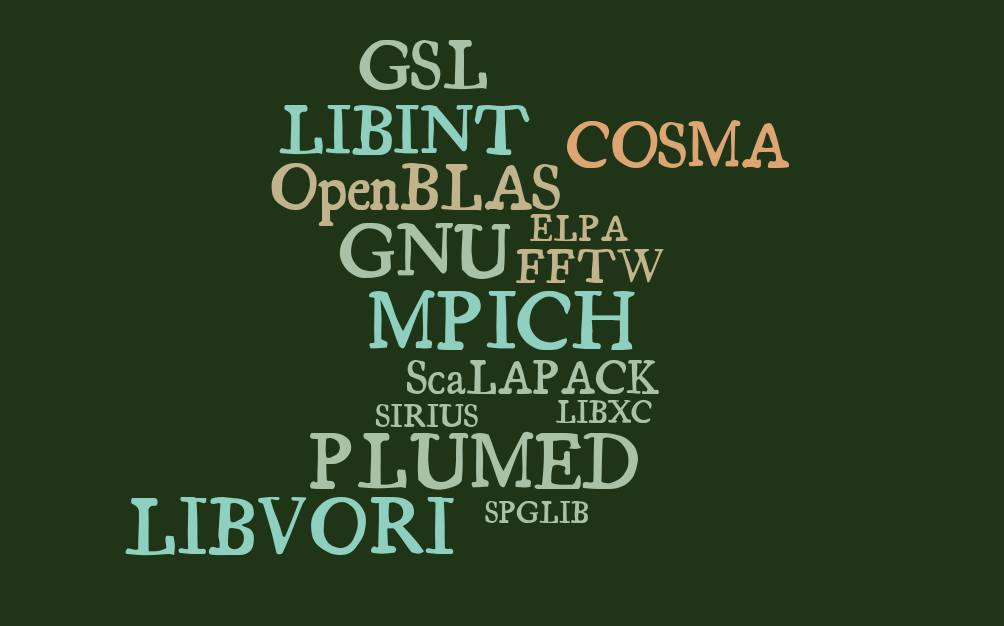
\includegraphics[width=0.7\linewidth]{fig/cp2k-lib.jpg}
  \caption{ไลบรารี่ที่โปรแกรม CP2K ใช้ในการช่วยคำนวณ}
  \label{fig:cp2k_lib}
\end{figure}

ผมจะอธิบาย Library ที่สำคัญ ๆ บางอันที่ CP2K ใช้ ดังนี้
%
\begin{description}
  \item[GNU] แน่นอนว่าเราต้องคอมไพล์ Source Code ดังนั้นเราจะต้องใช้ตัวคอมไพล์ (Compiler) ซึ่ง CP2K เลือกใช้ GNU เป็น Compiler

  \item[OpenBLAS กับ ScaLAPACK]  สำหรับ Linear Algebraic Calculation เช่น Matrix-vector, Matrix-matrix Multiplication

  \item[MPICH] อยากจะรันโปรแกรมแบบขนานโดยใช้ MPI ก็ต้องหา Implementation ที่จะมารันโค้ดของเรา ซึ่ง MPICH ก็เป็นหนึ่งใน Implementation ของ MPI ที่ CP2K เลือกใช้

  \item[FFTW] สำหรับทำฟูเรียร์ทรานฟอร์มในการคำนวณ DFT หรือแปลงจาก Real Space ไปเป็น Reciprocal Space สำหรับการคำนวณ Electrostatics โดยใช้ Plane Wave Electron Density

  \item[LIBXC] เป็น Library ที่ให้เราสามารถนำ DFT Functional มาใช้ได้เลยโดยไม่ต้อง Implement เอง
\end{description}

สรุปก็คือจะเห็นได้ว่าการเขียนโค้ดของโปรแกรมเคมีควอนตัมนั้นมีความซับซ้อนมากดังนั้นเรามีสองทางเลือกคือ
%
\begin{enumerate}[topsep=0pt,noitemsep]
  \setlength\itemsep{0.5em}
  \item ใช้ Library ที่มีอยู่แล้วสำหรับการทำงานเฉพาะจุด

  \item เขียนโค้ดทั้งหมดเองเลย
\end{enumerate}

แน่นอนว่าถ้าเราเลือกวิธีแรกก็จะประหยัดเวลาไปได้เยอะมากและเวลาที่เราคอมไพล์โปรแกรมก็ขอแค่ Link กับ Library ต่าง ๆ ก็รันโปรแกรมได้แล้วและทำให้ขนาดของตัวโปรแกรมของเรา (ขนาดของ Binary Files) นั้นมีขนาดไม่ใหญ่มากเกินไปด้วย (เช่นหลักสิบ-ร้อยเมกะไบต์)

อย่างไรก็ตามโปรแกรมสำหรับจำลองระบบโมเลกุลหลาย ๆ โปรแกรมก็ไม่ได้ใช้ Library เหล่านี้และเลือกใช้วิธีที่ 2 ก็คือการเขียนโค้ดสำหรับการคำนวณส่วนต่าง ๆ เองเลยเนื่องด้วยเหตุหลายข้อ เช่น การเขียนโค้ดทั้งหมดภายใน Framework โปรแกรมเดียวกันนั้นจะทำให้โค้ดมีประสิทธิภาพและทำงานร่วมกันได้ดี (Compatibility), ง่ายต่อการดูแลรักษาและปรับปรุงโค้ดเพราะว่า Developers นั้นรู้และเข้าใจการทำงานของโค้ดทั้งหมด, ถึงแม้ว่าโปรแกรมที่เขียนโค้ดทั้งหมดเองเมื่อถูกคอมไพล์แล้วจะได้ออกมาเป็น Binary File ที่มีขนาดนั้นใหญ่มาก ๆ เช่น หลายกิกะไบต์ แต่ว่าก็มีความคล่องตัวในการใช้งานเพราะว่าไม่ต้องติดตั้ง Library อื่น ๆ เพิ่มเติม

นอกจากนี้แล้วการที่ใช้ Library หลาย ๆ ตัวแบบนี้ก็มีจุดอ่อนบางข้อที่เราควรจะต้องรู้ไว้นั่นก็คือการเข้ากันได้ (Compatibility) ระหว่าง Library หรือเวอร์ชันซึ่งก็อาจจะทำให้เราปวดหัวได้ถ้าหากว่า Library บางตัวมีการอัพเดทเวอร์ชันใหม่แล้ว Conflict กับ Library ตัวอื่น

%----------------------------------------
\section{ทักษะและเครื่องมือสำหรับการเขียนโปรแกรมคำนวณทางวิทยาศาสตร์}
%----------------------------------------

\noindent \textbf{ภาษาคอมพิวเตอร์}
%
\begin{itemize}[topsep=0pt,noitemsep]
  \setlength\itemsep{0.5em}
  \item ภาษาสคริปต์ (Scripting Language): Bash, Python

  \item ภาษาระดับล่างที่เป็น Object-Oriented Programming: \cpp, Fortran

  \item ภาษาเชิงสัญลักษณ์ (Symbolic Programming): Mathematica, SymPy
\end{itemize}

\noindent \textbf{โปรแกรมสำหรับการเขียนโค้ด}
%
\begin{itemize}[topsep=0pt,noitemsep]
  \setlength\itemsep{0.5em}
  \item Vi/Vim, Nano

  \item VS Code, Atom, Eclipse, Sublime, Notepad++
\end{itemize}

\noindent \textbf{พื้นฐานการเขียนโปรแกรม}
%
\begin{itemize}[topsep=0pt,noitemsep]
  \setlength\itemsep{0.5em}
  \item ชนิดของตัวแปร (Variable Types)

  \item ตัวดำเนินการหรือโอเปอร์เรเตอร์ (Operator)

  \item Control Statements เช่น For, Do, If-Else, Case

  \item ฟังก์ชัน (Function)

  \item Vairable Scope และ Reference Types

  \item คลาส (Class) และวัตถุ (Objects)
\end{itemize}

\noindent \textbf{ภาษาคอมพิวเตอร์ระดับล่าง}

\noindent \underline{ภาษา C}
%
\begin{itemize}[topsep=0pt,noitemsep]
  \setlength\itemsep{0.5em}
  \item Function, Pointer, Storage Class

  \item Enum, Struct, Union

  \item Preprocessor

  \item Operator, Memory Management, Array

  \item การจัดการไฟล์ (File Handling)
\end{itemize}

\noindent \textbf{ภาษาคอมพิวเตอร์ระดับสูง}

\noindent \underline{ภาษา Python}
%
\begin{itemize}[topsep=0pt,noitemsep]
  \item Pip และ Conda: ตัวช่วยจัดการไลบรารี่ของ Python

  \item NumPy: จัดการและคำนวณ Array (เวกเตอร์, เมทริกซ์)

  \item Numba: JIT Compiler สำหรับ NumPy

  \item Jax: ทำ Autograd (Gradient Comptuation) สำหรับ NumPy Array

  \item SciPy: ไลบรารี่ที่รวมรวบฟังก์ชันทางคณิตศาสตร์และวิทยาศาสตร์

  \item Scikit-learn: ไลบรารี่สำหรับทำสถิติ, Optimization, และ Curve Fitting รวมถึง Machine Learning

  \item Matplotlib, Plotly: พลอตกราฟ

  \item Theano: คำนวณเชิงตัวเลข (Numerical Computation)

  \item SCOOP: โมดูลสำหรับการทำโปรแกรมแบบขนาน (Parallel Programming)

  \item NetworkX: ไลบรารี่สำหรับ Graph
\end{itemize}

\noindent \underline{ภาษา \cpp}
%
\begin{itemize}[topsep=0pt,noitemsep]
  \item Type of variable: \ih{signed}, \ih{unsigned}, \ih{long}, \ih{double} และอื่น ๆ

  \item Loops, Conditional Statement

  \item Standard libraries: \ih{vector}, \ih{rand}

  \item เข้าใจ Header (\ih{.hpp}) และ Source File (\texttt{.cpp} or \texttt{.cc})

  \item Preprocessor (\texttt{\#if}, \texttt{\#ifdef}, \texttt{\#ifndef}, \texttt{\#define}, etc.)

  \item Function, Class, Struct, Template

  \item Declaration

  \item Namespace, Const, Attribute, Pointer, Pass by Reference, \ih{static_assert}

  \item Initialization

  \item Casting, Lambda Expression, Encapsulation, File Handling, Exception Handling
\end{itemize}

\noindent \underline{ภาษา Fortran}
%
\begin{itemize}[topsep=0pt,noitemsep]
  \item เรียนรู้ภาษา Fortran ที่เป็น Modern Fortran ตั้งแต่เวอร์ชัน 2003 เป็นต้นไป

  \item โมดูล (Module), โปรแกรมย่อยหรือซับรูทีน (Subroutine), ฟังก์ชัน (Function)

  \item Array ทั้งแบบที่ปรับเปลี่ยนได้ (Allocatable) และแบบหลายมิติ (Multidimentional)

  \item Operator Overloading, Flow control

  \item Derived Type

  \item Callback

  \item การเขียนโปรแกรมเชื่อมโยงกับภาษาอื่น เช่น Python หรือ \cpp

  \item การใช้ GNU Library ในการคอมไพล์

  \item การจัดการหน่วยความจำ (Memory Allocation): Stack, Heap, Global Memory
\end{itemize}

\noindent \underline{ไลบรารี่สำหรับการคำนวณทางคณิตศาสตร์}
%
\begin{itemize}[topsep=0pt,noitemsep]
  \item BLAS (OpenBLAS)

  \item LAPACK: สำหรับคำนวณ Linear Algebra

  \item ScaLAPACK: เป็น LAPACK สำหรับซุปเปอร์คอมพิวเตอร์

  \item Intel MKL (Intel oneAPI)

  \item FFTW: สำหรับคำนวณ Discrete Fourier Transform ในหนึ่งมิติหรือมากกว่าหนึ่งมิติก็ได้

  \item Eigen: สำหรับคำนวณ Linear Algebra

  \item Boost: ไลบรารี่ที่รวบรวมฟังก์ชันต่าง ๆ สำหรับช่วยเขียนโปรแกรมภาษา \cpp เช่น regex, serialization
\end{itemize}

\noindent \underline{เครื่องมือช่วยการพัฒนาซอฟต์แวร์}
%
\begin{itemize}[topsep=0pt,noitemsep]
  \item การทำ Code Optimization

  \item การทำ Benchmarking และ Scaling

  \item ความซับซ้อนเชิงการคำนวณ (Computational Complexity)

  \item Static และ Dynamic Libraries

  \item คอมไพเลอร์ Compiling (g++, gcc) และ Linking (ld)

  \item เครื่องมือสำหรับช่วยการคอมไพล์โค้ด: autoconf, configure, make, cmake, automake

  \item เครื่องมือสำหรับช่วยการ Debug: gdb สำหรับการ Debug ทั่วไปและ Valgrind สำหรับการวิเคราะห์ Memory Leak

  \item การทำ Source Code Control: Git (GitHub และ GitLab)

  \item การทำ Documentation: Sphinx (สำหรับ markdown และ reStructuredText), Doxygen
\end{itemize}

\noindent \underline{ไลบรารี่สำหรับเคมีควอนตัม}
%
\begin{itemize}[topsep=0pt,noitemsep]
  \item libxc: ไลบรารี่ที่รวบรวม XC Function สำหรับ DFT ซึ่งเราสามารถนำมาใช้งานได้เลย

  \item libint: ไลบรารี่ที่ช่วยในการคำนวณ Gaussian Integrals

  \item libcint: ไลบรารี่ที่ช่วยในการคำนวณ GTO Integrals
\end{itemize}

%----------------------------------------
\section{เขียนโปรแกรมวิเคราะห์ Molecular Geometry (ภาษา \cpp)}
%----------------------------------------

โปรแกรมแรกที่ผู้อ่านจะได้ศึกษาและฝึกเขียนตามก็คือโปรแกรมสำหรับวิเคราะห์เรขาคณิตเชิงโครงสร้าง Structural Geometry ของโมเลกุล โดยเราจะใช้ภาษา \cpp กันครับ ซึ่งภาษา \cpp นั้นเป็นภาษาที่มีประสิทธิภาพสูงมากและถูกใช้อย่างแพร่หลายในการทำงานวิจัยเคมีควอนตัม (รวมถึงสาขาอื่น ๆ ด้วย) และโปรแกรมสำหรับการวิเคราะห์อันนี้ไม่มีความซับซ้อนมาก

\noindent \bful{Step 1: อ่านไฟล์ Coordinates}

\vspace{5pt}

\begin{lstlisting}[style=MyC++]
#include <iostream>
#include <fstream>
#include <iomanip>
#include <cstdio>

using namespace std;

int main() 
{
  ifstream input("geom.dat");

  int natom;
  input >> natom;

  int *zval = new int[natom];
  double *x = new double[natom];
  double *y = new double[natom];
  double *z = new double[natom];

  for(int i=0; i < natom; i++)
    input >> zval[i] >> x[i] >> y[i] >> z[i];
  
  input.close();

  cout << "Number of atoms: " << natom << endl;
  cout << "Input Cartesian coordinates:\n";
  for(int i=0; i < natom; i++)
    printf("%d %20.12f %20.12f %20.12f\n", (int) zval[i], x[i], y[i], z[i]);

  delete[] zval;
  delete[] x;  delete[] y;  delete[] z;

  return 0;
}
\end{lstlisting}

\vspace{5pt}

จากตัวอย่างโค้ดด้านบนนั้นเริ่มการทำงานด้วยการอ่านไฟล์ Coordinates ของอะตอมในโมเลกุลซึ่งมีหน่วยคือ bohr โดยผู้อ่านอาจจะลองใช้ตัวอย่างโมเลกุลเล็ก ๆ เช่น Acetaldehyde ซึ่งมี Coordinates ดังนี้
%
\begin{Verbatim}[frame=single]
  7
  6  0.000000000000     0.000000000000     0.000000000000
  6  0.000000000000     0.000000000000     2.845112131228
  8  1.899115961744     0.000000000000     4.139062527233
  1 -1.894048308506     0.000000000000     3.747688672216
  1  1.942500819960     0.000000000000    -0.701145981971
  1 -1.007295466862    -1.669971842687    -0.705916966833
  1 -1.007295466862     1.669971842687    -0.705916966833
\end{Verbatim}
%
โดยที่เลข 7 ในบรรทัดแรกนั้นคือจำนวนอะตอมและบรรทัดที่เหลือนั้นคือพิกัดตำแหน่ง $x, y, z$ ของอะตอมแต่ละตัว เมื่อโปรแกรมเปิดไฟล์แล้วสิ่งที่จะทำต่อไปก็คือการอ่านข้อมูลแต่ละบรรทัดและเก็บข้อมูลไว้ จริง ๆ แล้วเราสามารถทำให้โค้ดตัวอย่างอันนี้มีความเป็นระเบียบมากขึ้นโดยการใช้ Class เช่น เราสามารถสร้างไฟล์ Header ที่ชื่อ \ih{molecule.h} แล้วทำการเรียกใช้งาน Class ในไฟล์โปรแกรม \ih{molecule.cpp} ได้ดังนี้

\vspace{5pt}

\begin{lstlisting}[style=MyC++]
#include "molecule.h"
#include <iostream>
#include <fstream>
#include <iomanip>
#include <cstdio>

using namespace std;

int main()
{
  Molecule mol("geom.dat", 0);

  cout << "Number of atoms: " << mol.natom << endl;
  cout << "Input Cartesian coordinates:\n";
  mol.print_geom();

  return 0;
}
\end{lstlisting}
%
\vspace{5pt}
%
ทีนี้สิ่งที่ผมอยากให้ผู้อ่านทำก็คือลองฝึกเขียนโค้ดของไฟล์ \ih{molecule.h} โดยดัดแปลงจากโค้ดด้านบนครับ

\noindent \bful{Step 2: คำนวณความยาวพันธะ (Bond Lengths)}

คำนวณระยะห่างระหว่างอะตอม (Interatomic Distances) โดยใช้สมการดังต่อไปนี้
%
\begin{equation}
  R_{ij}
  =
  \sqrt{
    (x_{i} - x_{j})^{2}
    + (y_{i} - y_{j})^{2}
    + (z_{i} - z_{j})^{2}
  }
\end{equation}
%
โดยที่ $x, y, z$ คือ Cartesian Coordinates และ $i$ กับ $j$ คือเลข Index ของอะตอม
%
สำหรับการเขียนโปรแกรมเพื่อคำนวณ Distance นั้น เราจะต้องคำนึงถึงการจัดการหน่วยความจำ (Memory Allocation) ด้วยเพื่อให้โปรแกรมนั้นมีประสิทธิภาพมากที่สุดซึ่งนั่นก็จะเกี่ยวข้องกับการเลือกวิธีในการเก็บข้อมูลของระยะห่างระหว่างอะตอม ในการหาความยาวระหว่างอะตอมของทุก ๆ คู่นั้นสามารถใช้เมทริกซ์มาเก็บข้อมูลได้ซึ่งขนาดของเมทริกซ์จะเป็น $N \times N$ โดยที่ $N$ คือจำนวนอะตอม ในการใช้เมทริกซ์นั้นเราจำเป็นที่จะต้องจัดสรร (Allocate) หน่วยความจำซึ่งทำได้สองวิธีคือ

\noindent $\bullet$ 1. ใช้ Static Two-Dimensional Array

\vspace{5pt}

\begin{lstlisting}[style=MyC++]
double R[50][50];
\end{lstlisting}

\vspace{5pt}

\noindent $\bullet$ 2. ใช้ Dynamic Allocation โดยการใช้คลาส \ih{Molecule}

\vspace{5pt}

\begin{lstlisting}[style=MyC++]
double **R = new double* [mol.natom];
for(int i=0; i < mol.natom; i++)
  R[i] = new double[mol.natom];
\end{lstlisting}
%
\vspace{5pt}
%
แล้วก็อย่าลืมลบหน่วยความจำหลังจากที่คำนวณเสร็จแล้วด้วย ดังนี้

\vspace{5pt}

\begin{lstlisting}[style=MyC++]
for(int i=0; i < mol.natom; i++)
  delete[] R[i];
delete[] R;
\end{lstlisting}

\vspace{5pt}

ขั้นตอนต่อไปก็คือการสร้างเมทริกซ์ขึ้นมาซึ่งสามารถทำได้โดยใช้ For Loop ในการวนไปเรื่อย ๆ ตามเลข Index ของอะตอม
%
\vspace{5pt}
%
แล้วก็อย่าลืมลบหน่วยความจำหลังจากที่คำนวณเสร็จแล้วด้วย ดังนี้

\vspace{5pt}

\begin{lstlisting}[style=MyC++]
...
#include <cmath>
...

for(int i=0; i < mol.natom; i++) {
  for(int j=0; j < mol.natom; j++) {
      R[i][j] = 
        sqrt(
          (mol.geom[i][0]-mol.geom[j][0])*(mol.geom[i][0]-mol.geom[j][0])
        + (mol.geom[i][1]-mol.geom[j][1])*(mol.geom[i][1]-mol.geom[j][1])
        + (mol.geom[i][2]-mol.geom[j][2])*(mol.geom[i][2]-mol.geom[j][2]) 
        );
  }
}
\end{lstlisting}

\vspace{5pt}

ลำดับต่อไปคือการแสดงค่าความยาวที่คำนวณได้โดยเราก็จะใช้ For Loop เหมือนเดิม

\vspace{5pt}

\begin{lstlisting}[style=MyC++]
for(int i=0; i < mol.natom; i++)
  for(int j=0; j < i; j++)
    printf("%d %d %8.5f\n", i, j, R[i][j]);
\end{lstlisting}

\vspace{5pt}

ขั้นตอนสุดท้ายคือการทำให้โค้ดนั้นมีความเรียบร้อยและมีประสิทธิภาพมากขึ้น โดยเราสามารถนำโค้ดด้านบนที่เราได้เขียนไว้สร้างเป็นฟังก์ชันใหม่ที่ชื่อว่า
\ih{bond()} ในคลาส \ih{Molecule} ได้ดังนี้

\vspace{5pt}

\begin{lstlisting}[style=MyC++]
double Molecule::bond(int a, int b)
{
  return sqrt( (geom[a][0]-geom[b][0])*(geom[a][0]-geom[b][0])
              + (geom[a][1]-geom[b][1])*(geom[a][1]-geom[b][1])
              + (geom[a][2]-geom[b][2])*(geom[a][2]-geom[b][2]) );
}
\end{lstlisting}

\vspace{5pt}

แล้วก็โปรแกรมของเราก็จะมีหน้าตาเป็นแบบนี้

\vspace{5pt}

\begin{lstlisting}[style=MyC++]
#include "molecule.h"
#include <iostream>
#include <fstream>
#include <iomanip>
#include <cstdio>
#include <cmath>

using namespace std;
  
int main()
{
  Molecule mol("geom.dat", 0);
  
  cout << "Number of atoms: " << mol.natom << endl;
  cout << "Input Cartesian coordinates:\n";
  mol.print_geom();
  
  cout << "\nInteratomic distances (bohr):\n";
  for(int i=0; i < mol.natom; i++)
    for(int j=0; j < i; j++)
      printf("%d %d %8.5f\n", i, j, mol.bond(i,j));
      
  return 0;
}
\end{lstlisting}
%
\vspace{5pt}
%
ซึ่งก็จะมีเอาต์พุตดังต่อไปนี้

\vspace{5pt}

\begin{lstlisting}[style=MyC++]
Number of atoms: 7
Input Cartesian coordinates:
6     0.000000000000     0.000000000000     0.000000000000
6     0.000000000000     0.000000000000     2.845112131228
8     1.899115961744     0.000000000000     4.139062527233
1    -1.894048308506     0.000000000000     3.747688672216
1     1.942500819960     0.000000000000    -0.701145981971
1    -1.007295466862    -1.669971842687    -0.705916966833
1    -1.007295466862     1.669971842687    -0.705916966833

Interatomic distances (bohr):
1 0  2.84511
2 0  4.55395
2 1  2.29803
3 0  4.19912
3 1  2.09811
3 2  3.81330
4 0  2.06517
4 1  4.04342
4 2  4.84040
4 3  5.87463
5 0  2.07407
5 1  4.05133
5 2  5.89151
5 3  4.83836
5 4  3.38971
6 0  2.07407
6 1  4.05133
6 2  5.89151
6 3  4.83836
6 4  3.38971
6 5  3.33994
\end{lstlisting}
%
\vspace{5pt}
%
โดยที่ \ih{bond()} คือ Member Function ของ \ih{Molecule} ซึ่งเราสามารถเรียกใช้ข้อมูลของ Geometry (Coordinates) ได้ผ่าน \ih{geom} โดยไม่จำเป็นต้องเรียกใช้ผ่าน \ih{mol.geom}

\noindent \bful{Step 3: คำนวณมุมพันธะ (Bond Angles)}

เราสามารถคำนวณมุมพันธะทุกมุมที่เป็นไปได้ทั้งหมดของโมเลกุล (ระหว่างอะตอม $i, j, k$) $\phi_{ijk}$ ได้ด้วยสมการดังต่อไปนี้
%
\begin{equation}
  \label{eq:cos_bond_angle}
  \cos \phi_{ijk} = \tilde{e}_{ji} \cdot \tilde{e}_{jk}
\end{equation}
%
โดยที่ $e_{ij}$ คือเวกเตอร์หนึ่งหน่วย (Unit Vector) ระหว่างอะตอมซึ่งสามารถคำนวณได้ด้วยสมการดังต่อไปนี้
%
\begin{align}
  e^{x}_{ij}
  = \frac{
    -(x_{i} - x_{j})
  }
  {
    R_{ij}
  } \\
  e^{y}_{ij}
  = \frac{
    -(y_{i} - y_{j})
  }
  {
    R_{ij}
  } \\
  e^{z}_{ij}
  = \frac{
    -(z_{i} - z_{j})
  }
  {
    R_{ij}
  }
\end{align}
%
\vspace{5pt}
%
โดยเราจะสร้างฟังก์ชันสำหรับคำนวณมุมพันธะซึ่งก็คือ Inverse ของฟังก์ชัน Cosine ของสมการที่ \eqref{eq:cos_bond_angle} แล้วเพิ่มฟังก์ชันนี้เข้าไปในไฟล์ \ih{molecule.cpp} ดังนี้

\vspace{5pt}

\begin{lstlisting}[style=MyC++]
// Returns the value of the unit vector between atoms a and b
// in the cart direction (cart=0=x, cart=1=y, cart=2=z)
double Molecule::unit(int cart, int a, int b)
{
  return -(geom[a][cart]-geom[b][cart])/bond(a,b);
}

// Returns the angle between atoms a, b, and c in radians
double Molecule::angle(int a, int b, int c)
{
  return acos(unit(0,b,a) * unit(0,b,c) + unit(1,b,a) * unit(1,b,c) + unit(2,b,a) * unit(2,b,c));
}
\end{lstlisting}
%
\vspace{5pt}
%
นอกจากนี้เราจะต้องเพิ่ม Declaration ของ Member Function เข้าไปในไฟล์ \ih{molecule.h} ด้วย ดังนี้

\vspace{5pt}

\begin{lstlisting}[style=MyC++]
#include <string>

using namespace std;

class Molecule
{
  public:
    int natom;
    int charge;
    int *zvals;
    double **geom;
    string point_group;

    void print_geom();
    void rotate(double phi);
    void translate(double x, double y, double z);
    double bond(int atom1, int atom2);
    double angle(int atom1, int atom2, int atom3);
    double torsion(int atom1, int atom2, int atom3, int atom4);
    double unit(int cart, int atom1, int atom2);

    Molecule(const char *filename, int q);
    ~Molecule();
};
\end{lstlisting}

\vspace{5pt}

แล้วโปรแกรมสำหรับคำนวณมุมพันธะที่สมบูรณ์นั้นจะมีหน้าตาแบบนี้

\vspace{5pt}

\begin{lstlisting}[style=MyC++]
#include "molecule.h"
#include <iostream>
#include <fstream>
#include <iomanip>
#include <cstdio>
#include <cmath>

using namespace std;
  
int main()
{
  Molecule mol("geom.dat", 0);
  
  cout << "Number of atoms: " << mol.natom << endl;
  cout << "Input Cartesian coordinates:\n";
  mol.print_geom();

  cout << "\nBond angles:\n";
  for(int i=0; i < mol.natom; i++) {
    for(int j=0; j < i; j++) {
      for(int k=0; k < j; k++) {
        if(mol.bond(i,j) < 4.0 && mol.bond(j,k) < 4.0)
          printf("%2d-%2d-%2d %10.6f\n", i, j, k, mol.angle(i,j,k)*(180.0/acos(-1.0)));
      }
    }
  }

  return 0;
}
\end{lstlisting}

\vspace{5pt}

\noindent โดยที่เราใช้ \cppinline{acos(-1.0)} ในการประมาณค่า $\pi$

เมื่อเรารันโปรแกรมด้านบนจะได้เอาต์พุตแบบนี้

\vspace{5pt}

\begin{lstlisting}
Number of atoms: 7
Input Cartesian coordinates:
6     0.000000000000     0.000000000000     0.000000000000
6     0.000000000000     0.000000000000     2.845112131228
8     1.899115961744     0.000000000000     4.139062527233
1    -1.894048308506     0.000000000000     3.747688672216
1     1.942500819960     0.000000000000    -0.701145981971
1    -1.007295466862    -1.669971842687    -0.705916966833
1    -1.007295466862     1.669971842687    -0.705916966833

Bond angles:
  2- 1- 0 124.268308
  3- 1- 0 115.479341
  3- 2- 1  28.377448
  5- 4- 0  35.109529
  6- 4- 0  35.109529
  6- 5- 0  36.373677
  6- 5- 4  60.484476
\end{lstlisting}

\vspace{5pt}

\noindent \bful{Step 4: คำนวณมุมบิด (Torsion หรือ Dihedral Angles)}

พารามิเตอร์ลำดับต่อไปที่เราจะคำนวณก็คือมุมบิด (Torsion Angle) สำหรับมุมบิดของอะตอม 4 อะตอมใด ๆ ในโมเลกุล $i, j, k, l$ นั้นมีสมการในการคำนวณคือ
%
\begin{equation}
  \cos \tau_{ijkl}
  =
  \frac{
    (\tilde{e}_{ij} \times \tilde{e}_{jk})
    \cdot
    (\tilde{e}_{jk} \times \tilde{e}_{kl})
  }
  {
    \sin \theta_{ijk}
    \sin \theta_{jkl}
  }
\end{equation}
%
สิ่งที่ต้องระวังในการคำนวณ Torsion Angle ก็คือเครื่องหมายของมุมซึ่งจะเป็นบวกหรือลบนั้นก็คือขึ้นอยู่กับว่าเวกเตอร์นั้นมีทิศทางไปทางไหนเมื่อเทียบกับระนาบ

\begin{itemize}[topsep=0pt,noitemsep]
  \setlength\itemsep{0.5em}
  \item มุมบิดของอะตอม $i-j-k-l$ เป็นบวกเมื่อเวกเตอร์ตามแนวอะตอม $k-l$ นั้นวางตัวไปทางด้านขวาของระนาบที่สร้างจากอะตอม $i-j-k$ เมื่อมองจากทิศทางของเวกเตอร์ $j-k$

  \item มุมบิดของอะตอม $i-j-k-l$ เป็นลบเมื่อเวกเตอร์ตามแนวอะตอม $k-l$ นั้นวางตัวไปทางด้านซ้ายของระนาบที่สร้างจากอะตอม $i-j-k$ เมื่อมองจากทิศทางของเวกเตอร์ $j-k$
\end{itemize}

\vspace{5pt}

โปรแกรมสำหรับคำนวณ Torsion Angle นั้นมีดังนี้ เริ่มต้นด้วยการสร้าง Member Function ของคลาส \ih{Molecule}

\vspace{5pt}

\begin{lstlisting}[style=MyC++]
// Computes the angle between planes a-b-c and b-c-d
double Molecule::torsion(int a, int b, int c, int d)
{
  double eabc_x = (unit(1,b,a)*unit(2,b,c) - unit(2,b,a)*unit(1,b,c));
  double eabc_y = (unit(2,b,a)*unit(0,b,c) - unit(0,b,a)*unit(2,b,c));
  double eabc_z = (unit(0,b,a)*unit(1,b,c) - unit(1,b,a)*unit(0,b,c));

  double ebcd_x = (unit(1,c,b)*unit(2,c,d) - unit(2,c,b)*unit(1,c,d));
  double ebcd_y = (unit(2,c,b)*unit(0,c,d) - unit(0,c,b)*unit(2,c,d));
  double ebcd_z = (unit(0,c,b)*unit(1,c,d) - unit(1,c,b)*unit(0,c,d));

  double exx = eabc_x * ebcd_x;
  double eyy = eabc_y * ebcd_y;
  double ezz = eabc_z * ebcd_z;

  double tau = (exx + eyy + ezz)/(sin(angle(a,b,c)) * sin(angle(b,c,d)));

  if(tau < -1.0) tau = acos(-1.0);
  else if(tau > 1.0) tau = acos(1.0);
  else tau = acos(tau);

  // Compute the sign of the torsion 
  double cross_x = eabc_y * ebcd_z - eabc_z * ebcd_y;
  double cross_y = eabc_z * ebcd_x - eabc_x * ebcd_z;
  double cross_z = eabc_x * ebcd_y - eabc_y * ebcd_x;
  double norm = cross_x*cross_x + cross_y*cross_y + cross_z*cross_z;
  cross_x /= norm;
  cross_y /= norm;
  cross_z /= norm;
  double sign = 1.0;
  double dot = cross_x*unit(0,b,c)+cross_y*unit(1,b,c)+cross_z*unit(2,b,c);
  if(dot < 0.0) sign = -1.0;

  return tau*sign;
}
\end{lstlisting}

\vspace{5pt}

แล้วเราก็เรียกใช้ฟังก์ชันใหม่ที่เราเพิ่งสร้างไว้ในโปรแกรมหลักของเราได้ดังนี้

\vspace{5pt}

\begin{lstlisting}[style=MyC++]
#include <iostream>
#include <fstream>
#include <iomanip>
#include <cstdio>
#include <cmath>
#include "molecule.h"

using namespace std;

int main()
{
  Molecule mol("geom.dat", 0);

  cout << "Number of atoms: " << mol.natom << endl;
  cout << "Input Cartesian coordinates:\n";
  mol.print_geom();

  cout << "\nTorsional angles:\n";
  for(int i=0; i < mol.natom; i++) {
    for(int j=0; j < i; j++) {
      for(int k=0; k < j; k++) {
        for(int l=0; l < k; l++) {
          if(mol.bond(i,j) < 4.0 && mol.bond(j,k) < 4.0 && mol.bond(k,l) < 4.0)
            printf("%2d-%2d-%2d-%2d %10.6f\n", i, j, k, l, mol.torsion(i,j,k,l)*(180.0/acos(-1.0)));
        }
      }
    }
  }

  return 0;
}
\end{lstlisting}
%
\vspace{5pt}
%
เมื่อเรารันโปรแกรมด้านบนเราจะได้เอาต์พุตดังนี้

\vspace{5pt}

\begin{lstlisting}[style=MyC++]
Number of atoms: 7
Input Cartesian coordinates:
6       0.000000000000       0.000000000000       0.000000000000
6       0.000000000000       0.000000000000       2.845112131228
8       1.899115961744       0.000000000000       4.139062527233
1      -1.894048308506       0.000000000000       3.747688672216
1       1.942500819960       0.000000000000      -0.701145981971
1      -1.007295466862      -1.669971842687      -0.705916966833
1      -1.007295466862       1.669971842687      -0.705916966833

Torsional angles:
  3- 2- 1- 0 180.000000
  6- 5- 4- 0  36.366799  
\end{lstlisting}

\vspace{5pt}

\noindent \bful{Step 5: คำนวณจุดศูนย์กลางมวล มุมบิด (Center of Mass)}

\noindent \underline{แบบฝึกหัด}: ให้ลองเขียนโปรแกรมคำนวณจุดศูนย์กลางมวลของโมเลกุล โดยสมการที่ใช้ในการคำนวณนั้นสามารถดูได้จาก
Wikipedia ครับ

\noindent \underline{เฉลย}

\vspace{5pt}

\begin{lstlisting}[style=MyC++]
#include "molecule.h"
#include "masses.h"

#include <iostream>
#include <fstream>
#include <iomanip>
#include <cstdio>
#include <cmath>

using namespace std;

int main()
{
  Molecule mol("geom.dat", 0);

  cout << "Number of atoms: " << mol.natom << endl;
  cout << "Input Cartesian coordinates:\n";
  mol.print_geom();

  cout << "Interatomic distances (bohr):\n";
  for(int i=0; i < mol.natom; i++)
    for(int j=0; j < i; j++)
      printf("%d %d %8.5f\n", i, j, mol.bond(i,j));

  cout << "\nBond angles:\n";
  for(int i=0; i < mol.natom; i++) {
    for(int j=0; j < i; j++) {
      for(int k=0; k < j; k++) {
        if(mol.bond(i,j) < 4.0 && mol.bond(j,k) < 4.0)
          printf("%2d-%2d-%2d %10.6f\n", i, j, k, mol.angle(i,j,k)*(180.0/acos(-1.0)));
      }
    }
  }

  cout << "\nOut-of-Plane angles:\n";
  for(int i=0; i < mol.natom; i++) {
    for(int k=0; k < mol.natom; k++) {
      for(int j=0; j < mol.natom; j++) {
        for(int l=0; l < j; l++) {
          if(i!=j && i!=k && i!=l && j!=k && k!=l && mol.bond(i,k) < 4.0 && 
              mol.bond(k,j) < 4.0 && mol.bond(k,l) < 4.0)
              printf("%2d-%2d-%2d-%2d %10.6f\n", i, j, k, l, mol.oop(i,j,k,l)*(180.0/acos(-1.0)));
        }
      }
    }
  }

  cout << "\nTorsional angles:\n\n";
  for(int i=0; i < mol.natom; i++) {
    for(int j=0; j < i; j++) {
      for(int k=0; k < j; k++) {
        for(int l=0; l < k; l++) {
          if(mol.bond(i,j) < 4.0 && mol.bond(j,k) < 4.0 && mol.bond(k,l) < 4.0)
            printf("%2d-%2d-%2d-%2d %10.6f\n", i, j, k, l, mol.torsion(i,j,k,l)*(180.0/acos(-1.0)));
        }
      }
    }
  }
  
  /* find the center of mass (COM) */
  double M = 0.0;
  for(int i=0; i < mol.atom; i++) M += an2masses[(int) mol.zvals[i]];

  double xcm=0.0;
  double ycm=0.0;
  double zcm=0.0;
  double mi;
  for(int i=0; i < mol.atom; i++) {
    mi = an2masses[(int) mol.zvals[i]];
    xcm += mi * mol.geom[i][0];
    ycm += mi * mol.geom[i][1];
    zcm += mi * mol.geom[i][2];
  }
  xcm /= M;
  ycm /= M;
  zcm /= M;
  printf("\nMolecular center of mass: %12.8f %12.8f %12.8f\n", xcm, ycm, zcm);

  mol.translate(-xcm, -ycm, -zcm);

  return 0;
}
\end{lstlisting}
%
\vspace{5pt}
%
เมื่อเรารันโปรแกรมด้านบนเราจะได้เอาต์พุตดังนี้

\vspace{5pt}

\begin{lstlisting}[style=MyC++]
Number of atoms: 7
Input Cartesian coordinates:
6       0.000000000000       0.000000000000       0.000000000000
6       0.000000000000       0.000000000000       2.845112131228
8       1.899115961744       0.000000000000       4.139062527233
1      -1.894048308506       0.000000000000       3.747688672216
1       1.942500819960       0.000000000000      -0.701145981971
1      -1.007295466862      -1.669971842687      -0.705916966833
1      -1.007295466862       1.669971842687      -0.705916966833
Interatomic distances (bohr):
1 0  2.84511
2 0  4.55395
2 1  2.29803
3 0  4.19912
3 1  2.09811
3 2  3.81330
4 0  2.06517
4 1  4.04342
4 2  4.84040
4 3  5.87463
5 0  2.07407
5 1  4.05133
5 2  5.89151
5 3  4.83836
5 4  3.38971
6 0  2.07407
6 1  4.05133
6 2  5.89151
6 3  4.83836
6 4  3.38971
6 5  3.33994

Bond angles:
  0- 1- 2 124.268308
  0- 1- 3 115.479341
  0- 4- 5  35.109529
  0- 4- 6  35.109529
  0- 5- 6  36.373677
  1- 2- 3  28.377448
  4- 5- 6  60.484476

Out-of-plane angles:
  0- 3- 1- 2  -0.000000
  0- 6- 4- 5  19.939726
  0- 6- 5- 4 -19.850523
  0- 5- 6- 4  19.850523
  1- 5- 0- 4  53.678778
  1- 6- 0- 4 -53.678778
  1- 6- 0- 5  54.977064
  2- 3- 1- 0   0.000000
  3- 2- 1- 0  -0.000000
  4- 5- 0- 1 -53.651534
  4- 6- 0- 1  53.651534
  4- 6- 0- 5 -54.869992
  4- 6- 5- 0  29.885677
  4- 5- 6- 0 -29.885677
  5- 4- 0- 1  53.626323
  5- 6- 0- 1 -56.277112
  5- 6- 0- 4  56.194621
  5- 6- 4- 0 -30.558964
  5- 4- 6- 0  31.064344
  6- 4- 0- 1 -53.626323
  6- 5- 0- 1  56.277112
  6- 5- 0- 4 -56.194621
  6- 5- 4- 0  30.558964
  6- 4- 5- 0 -31.064344

Torsional angles:

  3- 2- 1- 0 180.000000
  6- 5- 4- 0  36.366799

Molecular center of mass:   0.64494926   0.00000000   2.31663792
\end{lstlisting}

%----------------------------------------
\section{เขียนโปรแกรม Hartree-Fock SCF (ภาษา Python)}
%----------------------------------------
\idxboth{วิธีฮาร์ทรี-ฟ็อค}{Hartree-Fock Method}

%----------------------------------------
\subsection{ทำความเข้าใจขั้นตอน SCF กันก่อน}
%----------------------------------------

โปรแกรมเคมีควอนตัมทุกโปรแกรมจะต้องมีส่วนหนึ่งของโปรแกรมที่เป็นโค้ดสำหรับแก้สมการอันหนึ่งซึ่งขาดไม่ได้เลยนั่นก็คือ Roothaan-Hall Equation โดยใช้วิธี Self-Consistent Field ซึ่งเป็นสมการที่เราใช้ในการคำนวณหาพลังงานของระบบที่เราสนใจ

สมการ Roothaan-Hall นั้นจะเรียกว่าเป็นสมการ HF ที่แปลงร่างมาแล้วก็ได้ สาเหตุที่เราต้องทำการแปลงร่าง HF นั้นก็เพราะว่าเราเขียน Wavefunction ให้อยู่ในรูปที่มี Basis Function นั่นเอง (Basis Function คือสิ่งที่เราใช้อธิบายออร์บิทัลเชิงอะตอม) โดยเราจะมีสมการ Roothaan-Hall ทั้งหมด $m$ สมการ โดยที่ $m$ คือจำนวนของ Basis Function (เรามีสมการ HF 1 สมการต่อ 1 MO และการที่เรามี $m$ Basis Function นั้นก็จะสร้างทั้งหมด $m$ MOs ด้วย), $F$ คือ Fock Matrix ซึ่งก็จะได้จาก Density Matrix แล้ว Density Matrix ก็คือ Matrix ที่มีสมาชิกเป็นผลคูณระหว่าง Coefficients ของ MO ซึ่งก็จะได้มาจากการประมาณค่าด้วยวิธีเริ่มต้น (Initial Guess) แบบต่าง ๆ เช่นใช้ H\"{u}ckel Method, ส่วน $S$ นั้นก็คือ Overlap Matrix ซึ่งก็จะเป็น Matrix ที่บอกว่า Orbitals นั้นสัมพันธ์กันมากน้อยแค่ไหน, และ $\epsilon$ ของแต่ละสมการนั้นก็คือค่าพลังงานของแต่ละ MO นั้นเองซึ่งเป็นสิ่งที่เราต้องการแก้สมการหามันออกมา ทีนี้เราสามารถยุบรวมสมการ HF สำหรับแต่ละ Basis Function เข้าด้วยกันได้ ซึ่งจะได้ออกมาเป็นตามสมการที่สั้นและกระชับขึ้นนั่นก็คือสมการ Roothaan-Hall นั่นเอง ดังนี้ (เขียนในรูปของเมทริกซ์)
%
\begin{equation}
  \bm{FC} 
  = 
  \bm{SC \varepsilon}
\end{equation}
%
โดยมี $F$, $C$, และ $S$ แทน Fock Matrix, MO Coefficients Matrix, และ Overlap Matrix ตามลำดับ โดย Matrix ทั้งสามอันนี้มีขนาดคือ $m \times m$ แล้วก็ $\epsilon$ นั้นก็มีขนาด $m \times m$ ด้วย (มีเฉพาะสมาชิกในแนวทแยงเท่านั้นที่มีค่าไม่เท่ากับ 0) โดย $C$ มีหน้าตาดังต่อไปนี้
%
\begin{equation}
  \bm{C}
  =
  \left( \begin{matrix} c_{1,1} & c_{1,2} & ... & c_{1,m} \\
               c_{2,1} & c_{2,2} & ... & c_{2,m} \\
               \vdots  & \vdots  &     & \vdots  \\
               c_{m,1} & c_{m,2} & ... & c_{m,m}
    \end{matrix} \right)
\end{equation}
%
และ $\epsilon$
%
\begin{equation}
  \bm{E}
  =
  \left( \begin{matrix} \epsilon_1 & 0          & ... & 0            \\
               0          & \epsilon_2 & ... & 0            \\
               \vdots     & \vdots     &     & \vdots       \\
               0          & 0          & ... & \epsilon_{m}
    \end{matrix} \right)
\end{equation}
%
ซึ่งแนวคิดของการแก้ปัญหา SCF นั้นก็คือเราพยายามที่จะหาค่าของ $\bm{C}$ ที่จะทำให้มีพลังงานของระบบนั้นมีค่าน้อยที่สุดเท่าที่จะเป็นไปได้ (Energy Minimization) แต่ว่าเราดันมี $\bm{C}$ อยู่ทั้งสองข้างของสมการ ดังนั้นเราจึงต้องทำการแก้สมการด้านบนโดยการใช้การวนซ้ำ (Iteration) จนกว่าจะได้ $\bm{C}$ ของทั้งสองข้างของสมการที่เท่ากัน (หรือเกือบจะเท่ากัน) ซึ่งจะทำให้ได้ค่าพลังงาน $\epsilon$ ที่ต่ำที่สุดด้วย

ปัญหาถัดมาก็คือว่าสมการด้านบนนั้นมันเป็น Eigenvalue Problem ในฟอร์มที่ยังแก้ไม่ได้ (แก้ได้แต่ว่าจะได้คำตอบที่ไม่ถูกต้อง) ซึ่งถ้าหากเราสามารถเปลี่ยนจาก $\bm{FC} = \bm{SC \epsilon}$ ให้เป็น $\bm{FC} = \bm{C \epsilon}$ ได้ ก็จะทำให้เราสามารถแก้ Eigenvalue Problem ได้อย่างมีประสิทธิภาพและได้คำตอบที่ถูกต้อง ดังนั้นเราจึงมีเทคนิคในการแปลงโดยการทำ Orthogonalization ซึ่งถ้าสรุปสั้น ๆ ก็คือว่าเราสามารถ%
แปลงออกมาได้เป็น
%
\begin{equation}
  \bm{F'C'} 
  = 
  \bm{C'E}
\end{equation}
%
โดยที่
%
\begin{gather}
  \bm{F'} = \bm{S}^{-1/2}\bm{F}\bm{S}^{-1/2} \\
  \bm{C'} = \bm{S}^{-1/2}\boldsymbol{C}
\end{gather}
%
ตามวิชา Linear Algebra ถ้าเราต้องการหา Matrix ของ $\epsilon$ เราสามารถใช้วิธี Diagonalization กับสมการ Roothaan-Hall ได้เพราะว่าสมการนี้มันเป็น Eigenfunction ซึ่งกระบวนการที่จะใช้ในการแก้นั้นก็คือตามขั้นตอนต่อไปนี้

\noindent \textbf{กระบวนการ SCF แบบคร่าว ๆ ตามทฤษฎี}

\begin{enumerate}[topsep=0pt,noitemsep]
  \setlength\itemsep{0.5em}
  \item เรากำหนดตำแหน่งของอะตอมในโมเลกุล, ประจุ, และทำการเลือก Basis Set

  \item เริ่มคำนวณพลังงานจลน์และพลังงานศักย์ รวมไปถึง Overlap Integral

  \item คำนวณ Orthogonalizing Matrix โดยใช้ Overlap Matrix (Overlap Matrix ที่ถูกสร้างมาจาก Overlap Integral ที่ได้จากขั้นที่ 2 อีกที)

  \item คำนวณ Fock Matrix อันแรกเลยโดยใช้พลังงานจลน์และพลังงานศักย์แล้วก็ใช้ Initial Guess ที่ได้จาก Coefficients ของ Basis Set ที่กำหนดไว้ตั้งแต่ขั้นตอนที่ 1

  \item ใช้ Orthogonalizing Matrix เพื่อแปลง (Tranform) Fock Matrix ให้เป็น Matrix อันใหม่ (เรียกว่าเป็น $F'$ ก็แล้วกัน) ที่มันขึ้นอยู่กับ Orthogonal Set ของฟังก์ชันที่ได้มาจาก Basis Set ที่ถูกเซนเตอร์กับอะตอม (Atom-centered Basis Set)

  \item ทำการทำเมทริกซ์แนวทแยง (Diagonalize) Fock Matrix เพื่อหา Coefficient Matrix ที่ถูกแปลงมาแล้ว (เรียกว่า $C'$) ก็ได้แล้วก็หาพลังงานของแต่ละ MO ได้

  \item เปรียบเทียบ $C'$ และพลังงานกับค่าที่ได้จากรอบก่อนหน้านี้ ถ้าผลต่างยังไม่น้อยกว่า Cutoff ที่กำหนดไว้ก็ให้นำ Fock Matrix ที่ได้มาล่าสุดไปใช้ใหม่อีกครั้งหนึ่งในขั้นที่ 4 ทำวนไปเรื่อย ๆ จนได้คำตอบที่แม่นยำ
\end{enumerate}

สำหรับการกำหนด Basis Set นั้นก็คือการเลือกชุดค่าสัมประสิทธิ์ของออร์บิทัล (Wavefunction) ของธาตุแต่ละธาตุ จริง ๆ แล้ว Basis Set นั้นก็คือไฟล์ Text ที่มีรูปแบบ (Format) ที่แตกต่างกันไปตามโปรแกรมที่ใช้ เราสามารถดาวน์โหลดไฟล์ Basis Set ได้ที่เว็บไซต์ \url{https://www.basissetexchange.org/} ตัวอย่างเช่น Basis Set: aug-cc-PV7Z ของอะตอมคาร์บอน \url{https://www.basissetexchange.org/basis/aug-cc-pv7z/format/nwchem/?version=0&elements=6}

%----------------------------------------
\subsection{มาเขียนโปรแกรมคำนวณ SCF กันเถอะ}
%----------------------------------------

ในส่วนนี้ผู้อ่านจะได้ศึกษาการเขียนโปรแกรมคำนวณ SCF ด้วยภาษา Python ซึ่งโปรแกรมด้านล่างนี้เป็นโปรแกรมที่ดัดแปลงมาจากโปรแกรมคำนวณ SCF จากหนังสือ Modern Quantum Chemsitry: Introduction to Advanced Electronic Structure Theory เขียนโดย Attila Szabo และ Neil S. Ostlund\footnote{ซอร์สโค้ดของโปรแกรมต้นฉบับเขียนด้วยภาษา Fortran สามารถดูไฟล์ได้ที่ \url{http://www.ccl.net/cca/software/SOURCES/FORTRAN/szabo/}} ซึ่งเป็นโปรแกรมที่คำนวณพลังงานของโมเลกุล \ce{HeH^{+}} ซึ่งมี Electronic Configuration ที่เหมือนกันกับ \ce{H2} แต่จะมีความแตกต่างกันตรงที่ \ce{HeH^{+}} นั้นมีประจุ +2 อยู่ที่อะตอม \ce{He} ทำให้โมเลกุลนี้ไม่มีความสมมาตร จึงต้องทำการคำนวณด้วยวิธีการวนซ้ำ

\noindent \bful{Step 1: สร้างออร์บิทัล}

ขั้นตอนแรกสุดเลยในการเขียนโปรแกรม SCF ก็คือการสร้างออร์บิทัล ทำไมเราต้องสร้างออร์บิทัลก่อนล่ะ? ก็เพราะว่าเราออร์บิทัลนั้นจริง ๆ แล้วก็คือ \enquote{ฟังก์ชันคลื่นของอิเล็กตรอน 1 ตัว} นั่นเอง ซึ่งเราจะกำหนดให้มีเซทของออร์บิทัล 1 เซทที่ใช้ในการอธิบายโมเลกุลทั้งโมเลกุล โดยเราจะใช้ Atomic Orbitals ที่มีจุดศูนย์กลางอยู่ที่อะตอม และเรานำ Atomic Orbitals แต่ละอันมารวมกันให้เป็นฟังก์ชันคลื่นหรือ Delocalized Orbital ได้โดยการใช้ Linear Combination of Atomic Orbitals (LCAO) ดังนี้
%
\begin{equation}
  \psi_i(\boldsymbol{r}_i)
  =
  \sum^{K}_{\mu} c_{\mu} \phi_{\mu I}(\boldsymbol{r}_i)
\end{equation}
%
โดยที่ $K$ คือจำนวน Basis Functions, $i = 1, 2, \dots, K$, และ $c$ คือพารามิเตอร์ที่เราจะต้องทำการปรับเพื่อลดค่าพลังงานของระบบโมเลกุล

เนื่องจากว่าวิธีการ Hartree-Fock นั้นใช้หลักการ Variation ซึ่งเป็นการหาฟังก์ชันคลื่นของระบบที่มีค่าพลังงานที่ไม่ว่ายังไงก็จะต้องมีค่าสูงกว่าพลังงานจริงของระบบ ข้อดีของ Variational Method ก็คือเราสามารถปรับพารามิเตอร์อะไรก็ได้อย่างเป็นระบบเพื่อให้ได้ฟังก์ชันคลื่นที่มีความถูกต้องมากขึ้นและให้ค่าพลังงานที่ลู่เข้าหรือ Converged
\idxboth{วิธีฮาร์ทรี-ฟ็อค}{Hartree-Fock Method}

สำหรับ Atomic Orbitals ที่เราจะใช้นั้นมีชื่อเรียกว่า Slater Type Orbitals (STO) สำหรับออร์บิทัล $1s$ นั้นมีสมการดังต่อไปนี้

\begin{equation}
  \phi^{Slater}\left( \boldsymbol{r}\right)
  =
  \left( \zeta^3/\pi \right)^{1/2}e^{-\zeta \boldsymbol{r}}
\end{equation}
%
เราลองมาพลอต STO อันนี้กันเพื่อดูว่ามีหน้าตาเป็นยังไง เริ่มต้นโดยการอิมพอร์ตไลบารี่ที่เราต้องการก่อน

\vspace{5pt}

\begin{lstlisting}[style=MyPython]
%matplotlib inline
import math
import numpy as np
import scipy.special as sp
import matplotlib.pyplot as plt
\end{lstlisting}
%
\vspace{5pt}
%
สร้างฟังก์ชันสำหรับพลอต STO

\vspace{5pt}

\begin{lstlisting}[style=MyPython]
x = np.linspace(-5,5,num=1000)
r = abs(x)
zeta = 1.0
psi_STO = (zeta**3/np.pi)**(0.5)*np.exp(-zeta*r)

plt.figure(figsize=(4,3))
plt.plot(x,psi_STO)
\end{lstlisting}

\vspace{5pt}

Slater Type Orbitals (STO) นั้นจริง ๆ แล้วก็คือฟังก์ชันที่เป็นผลเฉลยของสมการชโรดิงเงอร์สำหรับไฮโดรเจนอะตอมนั่นเอง (อิเล็กตรอน 1 ตัว) แต่ว่าการคำนวณอินทิกรัลของ STO นั้นสิ้นเปลืองมาก วิธีหนึ่งที่เราใช้ในการประมาณฟังก์ชัน STO นั้นก็คือการใช้ผลรวมของ Contracted Gaussian Functions (CGF) ซึ่งการที่เราใช้ CGF แทนนั้นช่วยทำให้เราประหยัดเวลาในการคำนวณมากขึ้นเพราะว่าการคำนวณอินทิกรัลของผลคูณระหว่าง Gaussian Functions 2 อันนั้นค่อนข้างง่ายพอสมควร สมการต่อไปนี้คือ Gaussian Function (CGF) ของออร์บิทัล $1s$
%
\begin{equation}
  \phi^{GF}(\alpha)
  =
  (2\alpha/\pi)^{3/4}exp(-\alpha r^{2})
\end{equation}
%
และผลรวมของ CGF คือ
%
\begin{equation}
  \phi^{CGF}\left( \boldsymbol{r}\right)
  =
  \sum_n d_n\phi^{GF}_n(\alpha)
\end{equation}
%
ซึ่งเราใช้ Gaussian Functions 3 อันในการหา Approximation ของ STO นั่นเอง ดังนี้
%
\begin{equation}
  \phi^{CGF}_{STO-3G}\left( \boldsymbol{r}\right)
  =
  \sum^3_n d_n\phi^{GF}_n(\alpha)
\end{equation}

\vspace{5pt}

\begin{lstlisting}[style=MyPython]
# Coeff is the d_n variable in the equation above
Coeff = np.array(
    [[1.00000, 0.0000000, 0.000000], [0.678914, 0.430129, 0.000000], [0.444635, 0.535328, 0.154329]]
)

# Expon is the alpha variable in the equation above
Expon = np.array(
    [[0.270950, 0.000000, 0.000000], [0.151623, 0.851819, 0.000000], [0.109818, 0.405771, 2.227660]]
)

psi_CGF_STO1G = Coeff[0, 0] * (2 * Expon[0, 0] / np.pi) ** (0.75) * np.exp(-Expon[0, 0] * r**2)
psi_CGF_STO2G = (
    Coeff[1, 0] * (2 * Expon[1, 0] / np.pi) ** (0.75) * np.exp(-Expon[1, 0] * r**2)
    + Coeff[1, 1] * (2 * Expon[1, 1] / np.pi) ** (0.75) * np.exp(-Expon[1, 1] * r**2)
    + Coeff[1, 2] * (2 * Expon[1, 2] / np.pi) ** (0.75) * np.exp(-Expon[1, 2] * r**2)
)
psi_CGF_STO3G = (
    Coeff[2, 0] * (2 * Expon[2, 0] / np.pi) ** (0.75) * np.exp(-Expon[2, 0] * r**2)
    + Coeff[2, 1] * (2 * Expon[2, 1] / np.pi) ** (0.75) * np.exp(-Expon[2, 1] * r**2)
    + Coeff[2, 2] * (2 * Expon[2, 2] / np.pi) ** (0.75) * np.exp(-Expon[2, 2] * r**2)
)

# Plot the three functions
plt.figure(figsize=(5, 3))
plt.title("Approximations to a STO with CGF")
plt.plot(x, psi_STO, label="STO")
plt.plot(x, psi_CGF_STO1G, label="STO-1G")
plt.legend()
plt.figure(figsize=(5, 3))
plt.plot(x, psi_STO, label="STO")
plt.plot(x, psi_CGF_STO2G, label="STO-2G")
plt.legend()
plt.figure(figsize=(5, 3))
plt.plot(x, psi_STO, label="STO")
plt.plot(x, psi_CGF_STO3G, label="STO-3G")
plt.legend()
\end{lstlisting}

\vspace{5pt}

จะเห็นได้ว่ายิ่งจำนวนของ GF เพิ่มมากขึ้นเท่าไหร่ ฟังก์ชันนั้นก็จะมีความเข้าใกล้ความเป็น STO มากขึ้นเท่านั้น โดยตำแหน่งที่ $x = 0$ นั้นจะเห็นว่าเป็นตำแหน่งที่ Approximation นั้นแย่ที่สุด โดยเราจะเรียกบริเวณที่เป็นความคลาดเคลื่อนของ CGF จาก STO นี้ว่า Cusp

\noindent \bful{Step 2: เตรียมส่วนผสมสำหรับการคำนวณ SCF}

\noindent $\bullet$ Step 2.1: กำหนดตัวแปรที่จะใช้ในการเก็บข้อมูลทางควอนตัมของโมเลกุล

\vspace{5pt}

\begin{lstlisting}[style=MyPython]
# Make all variables 'global variables' accessible through out the whole program
global H, S, X, XT, TT, G, C, P, Oldp, F, Fprime, Cprime, E

H = np.zeros([2, 2])
S = np.zeros([2, 2])
X = np.zeros([2, 2])
XT = np.zeros([2, 2])
TT = np.zeros([2, 2, 2, 2])
G = np.zeros([2, 2])
C = np.zeros([2, 2])

P = np.zeros([2, 2])
Oldp = np.zeros([2, 2])
F = np.zeros([2, 2])
Fprime = np.zeros([2, 2])
Cprime = np.zeros([2, 2])
E = np.zeros([2, 2])

Energy = 0.0
Delta = 0.0

# Values below taken from 'Modern Quantum Chemistry' book
# Appendix B: Two-Electron Self-Consistent-Field Program
IOP = 2
N = 3
R = 1.4632
Zeta1 = 2.0925
Zeta2 = 1.24
Za = 2.0
Zb = 1.0
\end{lstlisting}

\vspace{5pt}

\noindent $\bullet$ Step 2.2: สร้างฟังก์ชันสำหรับคำนวณ Integrals ต่าง ๆ

การคำนวณ Integrals นั้นจะทำได้ง่ายขึ้นเยอะมาก ๆ เลยถ้าหากว่าเราใช้ฟังก์ชัน Gaussian ในการอธิบายออร์บิทัล ผมแนะนำให้ผู้อ่านศึกษา Appendix ของหนังสือ Modern Quantum Chemistry ครับซึ่งจะช่วยให้เข้าใจได้มากขึ้น

\vspace{5pt}

\begin{lstlisting}[style=MyPython]
def F0(t):
  """
  F function for 1s orbital
  """
  if t < 1e-6:
      return 1.0 - t / 3.0
  else:
      return 0.5 * (np.pi / t) ** 0.5 * sp.erf(t**0.5)
\end{lstlisting}
%
\vspace{5pt}
%
ฟังก์ชันสำหรับคำนวณ Overlap Matrix

\vspace{5pt}

\begin{lstlisting}[style=MyPython]
def S_int(A, B, Rab2):
  """
  Calculates the overlap between two gaussian functions
  """
  return (np.pi / (A + B)) ** 1.5 * np.exp(-A * B * Rab2 / (A + B))
\end{lstlisting}
%
\vspace{5pt}
%
ฟังก์ชันสำหรับคำนวณ Kinetic Energy Integrals

\vspace{5pt}

\begin{lstlisting}[style=MyPython]
def T_int(A, B, Rab2):
  """
  Calculates the kinetic energy integrals for un-normalised primitives
  """
  return (
      A
      * B
      / (A + B)
      * (3.0 - 2.0 * A * B * Rab2 / (A + B))
      * (np.pi / (A + B)) ** 1.5
      * np.exp(-A * B * Rab2 / (A + B))
  )
\end{lstlisting}
%
\vspace{5pt}
%
ฟังก์ชันสำหรับคำนวณ Nuclear Attraction Integrals

\vspace{5pt}

\begin{lstlisting}[style=MyPython]
def V_int(A, B, Rab2, Rcp2, Zc):
  """
  Calculates the un-normalised nuclear attraction integrals
  """
  V = 2.0 * np.pi / (A + B) * F0((A + B) * Rcp2) * np.exp(-A * B * Rab2 / (A + B))

  return -V * Zc
\end{lstlisting}
%
\vspace{5pt}
%
ฟังก์ชันสำหรับคำนวณความคลาดเคลื่อน

\vspace{5pt}

\begin{lstlisting}[style=MyPython]
def erf(t):
  """
  Approximation for the error function
  """
  P = 0.3275911
  A = [0.254829592, -0.284496736, 1.421413741, -1.453152027, 1.061405429]
  T = 1.0 / (1 + P * t)
  Tn = T
  Poly = A[0] * Tn

  for i in range(1, 5):
      Tn = Tn * T
      Poly = Poly * A[i] * Tn

  return 1.0 - Poly * np.exp(-t * t)
\end{lstlisting}
%
\vspace{5pt}
%
ฟังก์ชันสำหรับคำนวณ Two-Electron Integrals

\vspace{5pt}

\begin{lstlisting}[style=MyPython]
def TwoE(A, B, C, D, Rab2, Rcd2, Rpq2):
  """
  Calculate Two-Electron integrals
  A, B, C, D are the exponents alpha, beta, etc.
  Rab2 equals squared distance between center A and center B
  """
  return (
      2.0
      * (np.pi**2.5)
      / ((A + B) * (C + D) * np.sqrt(A + B + C + D))
      * F0((A + B) * (C + D) * Rpq2 / (A + B + C + D))
      * np.exp(-A * B * Rab2 / (A + B) - C * D * Rcd2 / (C + D))
  )
\end{lstlisting}
%
\vspace{5pt}
%
สร้างฟังก์ชันสำหรับเรียกใช้ฟังก์ชันด้านบนที่เราได้เขียนไว้ ประกาศตัวแปรทั้งหมดที่ต้องใช้และทำการรวม Integrals ทั้งหมด (เราจะเรียกใช้ฟังก์ชันนี้ภายหลัง)

\vspace{5pt}

\begin{lstlisting}[style=MyPython]
def Intgrl(N, R, Zeta1, Zeta2, Za, Zb):
  """
  Declares the variables and compiles the integrals
  """

  global S12, T11, T12, T22, V11A, V12A, V22A, V11B, V12B, V22B, V1111, V2111, V2121, V2211, V2221, V2222

  S12 = 0.0
  T11 = 0.0
  T12 = 0.0
  T22 = 0.0
  V11A = 0.0
  V12A = 0.0
  V22A = 0.0
  V11B = 0.0
  V12B = 0.0
  V22B = 0.0
  V1111 = 0.0
  V2111 = 0.0
  V2121 = 0.0
  V2211 = 0.0
  V2221 = 0.0
  V2222 = 0.0

  R2 = R * R

  # The coefficients for the contracted Gaussian functions are below
  Coeff = np.array(
      [[1.00000, 0.0000000, 0.000000], [0.678914, 0.430129, 0.000000], [0.444635, 0.535328, 0.154329]]
  )

  Expon = np.array(
      [[0.270950, 0.000000, 0.000000], [0.151623, 0.851819, 0.000000], [0.109818, 0.405771, 2.227660]]
  )
  D1 = np.zeros([3])
  A1 = np.zeros([3])
  D2 = np.zeros([3])
  A2 = np.zeros([3])

  # This loop constructs the contracted Gaussian functions
  for i in range(N):
      A1[i] = Expon[N - 1, i] * (Zeta1**2)
      D1[i] = Coeff[N - 1, i] * ((2.0 * A1[i] / np.pi) ** 0.75)
      A2[i] = Expon[N - 1, i] * (Zeta2**2)
      D2[i] = Coeff[N - 1, i] * ((2.0 * A2[i] / np.pi) ** 0.75)

  # Calculate one electron integrals
  # Centre A is first atom centre B is second atom
  # Origin is on second atom
  # V12A - off diagonal nuclear attraction to centre A etc.
  for i in range(N):
      for j in range(N):
          # Rap2 - squared distance between centre A and centre P
          Rap = A2[j] * R / (A1[i] + A2[j])
          Rap2 = Rap**2
          Rbp2 = (R - Rap) ** 2
          S12 = S12 + S_int(A1[i], A2[j], R2) * D1[i] * D2[j]
          T11 = T11 + T_int(A1[i], A1[j], 0.0) * D1[i] * D1[j]
          T12 = T12 + T_int(A1[i], A2[j], R2) * D1[i] * D2[j]
          T22 = T22 + T_int(A2[i], A2[j], 0.0) * D2[i] * D2[j]
          V11A = V11A + V_int(A1[i], A1[j], 0.0, 0.0, Za) * D1[i] * D1[j]
          V12A = V12A + V_int(A1[i], A2[j], R2, Rap2, Za) * D1[i] * D2[j]
          V22A = V22A + V_int(A2[i], A2[j], 0.0, R2, Za) * D2[i] * D2[j]
          V11B = V11B + V_int(A1[i], A1[j], 0.0, R2, Zb) * D1[i] * D1[j]
          V12B = V12B + V_int(A1[i], A2[j], R2, Rbp2, Zb) * D1[i] * D2[j]
          V22B = V22B + V_int(A2[i], A2[j], 0.0, 0.0, Zb) * D2[i] * D2[j]

  # Calculate two electron integrals

  for i in range(N):
      for j in range(N):
          for k in range(N):
              for l in range(N):
                  Rap = A2[i] * R / (A2[i] + A1[j])
                  Rbp = R - Rap
                  Raq = A2[k] * R / (A2[k] + A1[l])
                  Rbq = R - Raq
                  Rpq = Rap - Raq
                  Rap2 = Rap * Rap
                  Rbp2 = Rbp * Rbp
                  Raq2 = Raq * Raq
                  Rbq2 = Rbq * Rbq
                  Rpq2 = Rpq * Rpq
                  V1111 = (
                      V1111
                      + TwoE(A1[i], A1[j], A1[k], A1[l], 0.0, 0.0, 0.0) * D1[i] * D1[j] * D1[k] * D1[l]
                  )
                  V2111 = (
                      V2111
                      + TwoE(A2[i], A1[j], A1[k], A1[l], R2, 0.0, Rap2) * D2[i] * D1[j] * D1[k] * D1[l]
                  )
                  V2121 = (
                      V2121 + TwoE(A2[i], A1[j], A2[k], A1[l], R2, R2, Rpq2) * D2[i] * D1[j] * D2[k] * D1[l]
                  )
                  V2211 = (
                      V2211 + TwoE(A2[i], A2[j], A1[k], A1[l], 0.0, 0.0, R2) * D2[i] * D2[j] * D1[k] * D1[l]
                  )
                  V2221 = (
                      V2221
                      + TwoE(A2[i], A2[j], A2[k], A1[l], 0.0, R2, Rbq2) * D2[i] * D2[j] * D2[k] * D1[l]
                  )
                  V2222 = (
                      V2222
                      + TwoE(A2[i], A2[j], A2[k], A2[l], 0.0, 0.0, 0.0) * D2[i] * D2[j] * D2[k] * D2[l]
                  )
  return
\end{lstlisting}
%
\vspace{5pt}
%
สร้างฟังก์ชันสำหรับนำ Integrals ที่คำนวณได้ใส่เข้าไปใน Array (เราจะเรียกใช้ฟังก์ชันนี้ภายหลัง)

\vspace{5pt}

\begin{lstlisting}[style=MyPython]
def Collect():
  """
  Takes the basic integrals and assembles the relevant matrices,
  that are S, H, X, XT and two electron integrals
  """
  # Form core hamiltonian
  H[0, 0] = T11 + V11A + V11B
  H[0, 1] = T12 + V12A + V12B
  H[1, 0] = H[0, 1]
  H[1, 1] = T22 + V22A + V22B

  # Form overlap matrix
  S[0, 0] = 1.0
  S[0, 1] = S12
  S[1, 0] = S12
  S[1, 1] = 1.0

  # This is S^-1/2
  X[0, 0] = 1.0 / np.sqrt(2.0 * (1.0 + S12))
  X[1, 0] = X[0, 0]
  X[0, 1] = 1.0 / np.sqrt(2.0 * (1.0 - S12))
  X[1, 1] = -X[0, 1]

  # This is the coulomb and exchange term (aa|bb) and (ab|ba)
  TT[0, 0, 0, 0] = V1111
  TT[1, 0, 0, 0] = V2111
  TT[0, 1, 0, 0] = V2111
  TT[0, 0, 1, 0] = V2111
  TT[0, 0, 0, 1] = V2111
  TT[1, 0, 1, 0] = V2121
  TT[0, 1, 1, 0] = V2121
  TT[1, 0, 0, 1] = V2121
  TT[0, 1, 0, 1] = V2121
  TT[1, 1, 0, 0] = V2211
  TT[0, 0, 1, 1] = V2211
  TT[1, 1, 1, 0] = V2221
  TT[1, 1, 0, 1] = V2221
  TT[1, 0, 1, 1] = V2221
  TT[0, 1, 1, 1] = V2221
  TT[1, 1, 1, 1] = V2222
\end{lstlisting}

\vspace{5pt}

\noindent \bful{Step 3: สร้างตัวคำนวณ SCF Calculator}

\vspace{5pt}

สร้างฟังก์ชันสำหรับการทำ Diagonalization ของ Fock Matrix ซึ่งเราจะได้ Eigenvectors และ Eigenvalues ออกมา ซึ่งก็คือ Array C กับ Array E ตามลำดับ

\vspace{5pt}

\begin{lstlisting}[style=MyPython]
def Diag(Fprime, Cprime, E):
  """
  Diagonalises F to give eigenvectors in C and eigenvalues in E
  theta is the angle describing the solution
  """
  # Angle for heteronuclear diatonic
  Theta = 0.5 * math.atan(2.0 * Fprime[0, 1] / (Fprime[0, 0] - Fprime[1, 1]))
  # print('Theta', Theta)

  Cprime[0, 0] = np.cos(Theta)
  Cprime[1, 0] = np.sin(Theta)
  Cprime[0, 1] = np.sin(Theta)
  Cprime[1, 1] = -np.cos(Theta)

  E[0, 0] = (
      Fprime[0, 0] * np.cos(Theta) ** 2
      + Fprime[1, 1] * np.sin(Theta) ** 2
      + Fprime[0, 1] * np.sin(2.0 * Theta)
  )
  E[1, 1] = (
      Fprime[1, 1] * np.cos(Theta) ** 2
      + Fprime[0, 0] * np.sin(Theta) ** 2
      - Fprime[0, 1] * np.sin(2.0 * Theta)
  )

  if E[1, 1] <= E[0, 0]:
      Temp = E[1, 1]
      E[1, 1] = E[0, 0]
      E[0, 0] = Temp
      Temp = Cprime[0, 1]
      Cprime[0, 1] = Cprime[0, 0]
      Cprime[0, 0] = Temp
      Temp = Cprime[1, 1]
      Cprime[1, 1] = Cprime[1, 0]
      Cprime[1, 0] = Temp
  return
\end{lstlisting}

\vspace{5pt}

\noindent ฟังก์ชันสุดท้ายคือฟังก์ชันที่จะเป็นการรันการคำนวณ SCF

\vspace{5pt}

\begin{lstlisting}[style=MyPython]
def SCF(R, Za, Zb, G):
  """
  Performs the SCF iterations
  """
  Crit = 1e-11  # Convergence critera
  Maxit = 250  # Maximum number of iterations
  Iter = 0

  #--------
  # STEP 1. Guess an initial density matrix
  #--------
  # Use core hamiltonian for initial guess of F (P = 0)
  P = np.zeros([2, 2])

  Energy = 0.0

  while Iter < Maxit:
      Iter += 1

      #--------
      # STEP 2. Calculate the Fock matrix 
      #--------
      # Form two electron part of Fock matrix from P
      # This is the two electron contribution in the equations above
      G = np.zeros([2, 2])  
      for i in range(2):
          for j in range(2):
              for k in range(2):
                  for l in range(2):
                      G[i, j] = G[i, j] + P[k, l] * (TT[i, j, k, l] - 0.5 * TT[i, l, k, j])

      # Add core hamiltonian H^CORE to get Fock matrix
      F = H + G

      # Calculate the electronic energy
      Energy = np.sum(0.5 * P * (H + F))

      #--------
      # STEP 3. Calculate F' 
      # (remember S^-1/2 is X and S^1/2 is X.T) 
      #--------
      G = np.matmul(F, X)
      Fprime = np.matmul(X.T, G)

      #--------
      # STEP 4. Solve the eigenvalue problem 
      #--------
      # Diagonalise transformed Fock matrix
      Diag(Fprime, Cprime, E)

      #--------
      # STEP 5. Calculate the molecular orbitals coefficients 
      #--------
      # Transform eigen vectors to get matrix C
      C = np.matmul(X, Cprime)

      # STEP 6. Calculate the new density matrix from the old P 
      Oldp = np.array(P)
      P = np.zeros([2, 2])

      # Form new density matrix
      for i in range(2):
          for j in range(2):
              # Save present density matrix before creating a new one
              for k in range(1):
                  P[i, j] += 2.0 * C[i, k] * C[j, k]

      #--------
      # STEP 7. Check to see if the energy has converged 
      #--------
      Delta = 0.0
      # Calculate delta the difference between the old and 
      # new density matrix (Old P and new P)
      Delta = P - Oldp
      Delta = np.sqrt(np.sum(Delta**2) / 4.0)

      print("Step ", Iter, " Elec Energy", Energy, " Diff", Delta)

      # Check for convergence
      if Delta < Crit:
          # Add nuclear repulsion to get the total energy
          Energy_tot = Energy + Za * Zb / R
          print("")
          print("Calculation converged with electronic energy:", Energy)
          print("Calculation converged with total energy:", Energy_tot)
          print("Density matrix")
          print(P)
          print("Mulliken populations")
          print(np.matmul(P, S))
          print("Coeffients")
          print(C)

          break
\end{lstlisting}

\vspace{5pt}

\noindent \bful{Step 4: รันการคำนวณ SCF และตรวจสอบความถูกต้อง}

\vspace{5pt}

และแล้วเราก็มาถึงขั้นตอนสุดท้ายนั่นก็คือการรันการคำนวณ SCF โดยสรุปอีกครั้งหนึ่งว่าขั้นตอนการคำนวณนั้นมีอัลกอริทึมดังต่อไปนี้
%
\begin{enumerate}[topsep=0pt,noitemsep]
  \setlength\itemsep{0.5em}
  \item ทำการเดา Initial Density Matrix $\bm{P}$ โดยในตัวอย่างโค้ดของเรานั้นจะใช้ $\bm{P} = 0$ เพื่อความง่าย

  \item นำ $\bm{P}$ มาสร้าง Fock Matrix $\bm{F}$

  \item คำนวณ $\bm{F'} = \bm{S}^{-1/2}\bm{F}\bm{S}^{1/2}$

  \item แก้สมการ Eigenvalue Problem โดยการนำ Secular Equation $|\bm{F'} - \bm{E}\bm{I}| = 0$ มาทำ Diagonalization ซึ่งเราจะได้ $\bm{E}$ และ $\bm{C}$ ออกมา

  \item คำนวณ Density Matrix $\bm{P}$ อันใหม่จาก $\bm{C}$

  \item ตรวจสอบเงื่อนไขว่าพลังงานนั้น Converged แล้วหรือยัง ถ้าหากว่ายังไม่ Converged ให้วนซ้ำขั้นตอนด้านบน
\end{enumerate}

เราเริ่มด้วยการเรียกใช้ฟังก์ชัน \pyinline{Intgrl} เพื่อคำนวณ One-Electron Intregral และ One-Electron Integral และตามด้วยฟังก์ชัน \pyinline{Collect} และฟังก์ชัน \pyinline{SCF} ตามลำดับ

\vspace{5pt}

\begin{lstlisting}[style=MyPython]
# Calculate one and two electron integrals
Intgrl(N, R, Zeta1, Zeta2, Za, Zb)

# Put all integals into array
Collect()

# Perform the SCF calculation
SCF(R, Za, Zb, G)
\end{lstlisting}
%
\vspace{5pt}
%
เมื่อรันแล้วจะได้เอาต์พุตของการคำนวณ SCF ของระบบโมเลกุล \ce{HeH^{+}} ดังนี้

\vspace{5pt}

\begin{lstlisting}[style=MyPython]
Step  1  Elec Energy 0.0  Diff 0.8828668530136917
Step  2  Elec Energy -4.141862876133925  Diff 0.2791763040686421
Step  3  Elec Energy -4.22649189912899  Diff 0.029661780077229444
Step  4  Elec Energy -4.227522925343759  Diff 0.0023182848695558057
Step  5  Elec Energy -4.227529268100319  Diff 0.00017439769686161983
Step  6  Elec Energy -4.227529304014095  Diff 1.3079512369092073e-05
Step  7  Elec Energy -4.227529304216109  Diff 9.807146593527476e-07
Step  8  Elec Energy -4.227529304217244  Diff 7.353368030466615e-08
Step  9  Elec Energy -4.22752930421725  Diff 5.5135252472270695e-09
Step  10  Elec Energy -4.227529304217251  Diff 4.1340208808251866e-10
Step  11  Elec Energy -4.227529304217252  Diff 3.099665019964731e-11
Step  12  Elec Energy -4.227529304217252  Diff 2.3244357915420586e-12

Calculation converged with electronic energy: -4.227529304217252
Calculation converged with total energy: -2.86066216370331
Density matrix
[[1.28614168 0.54017322]
  [0.54017322 0.22687011]]
Mulliken populations
[[1.52963579 1.11992783]
  [0.64243955 0.47036421]]
Coeffients
[[ 0.80191698 -0.78226577]
  [ 0.33680121  1.06844537]]
\end{lstlisting}

\vspace{5pt}

จากผลการคำนวณด้านบนจะเห็นได้ว่าพลังงานของโมเลกุล \ce{HeH^{+}} ที่คำนวณออกมาได้นั้นมีค่าลดลงเรื่อย ๆ โดยผ่านการคำนวณ SCF ทั้งหมด 12 ครั้ง พลังงานรวมของโมเลกุลที่คำนวณได้คือ -2.86066216370331 Hartree

\noindent แหล่งความรู้สำหรับอ่านเพิ่มเติม
%
\begin{enumerate}[topsep=0pt,noitemsep]
  \setlength\itemsep{0.5em}
  \item ถ้าอยากศึกษาทฤษฎี Hartree-Fock รวมถึง Variational Principle และ Basis Sets ผมแนะนำให้อ่านเลคเชอร์โน๊ตของคอร์ส Advanced Computational Chemistry\footnote{\url{http://www.chem.helsinki.fi/~manninen/lecture_notes.pdf}}

  \item ถ้าอยากศึกษาการพิสูจน์ทฤษฎี Hartree-Fock แบบละเอียด ผมแนะนำให้อ่าน \enquote{Derivation of Hartree-Fock Theory} โดย Arvi Rauk\footnote{\url{https://onlinelibrary.wiley.com/doi/10.1002/0471220418.app0a}}

  \item ถ้าอยากศึกษาการคำนวณ Molecular Integrals แบบละเอียด ผมแนะนำให้อ่าน \enquote{Fundamentals of Molecular Integrals Evaluation} โดย Justin T. Fermann และ Edward F. Valeev
\end{enumerate}

%----------------------------------------
\section{เขียนโปรแกรม Direct Inversion of the Iterative Subspace}
\idxen{Direct Inversion of the Iterative Subspace}
\idxen{DIIS}
%----------------------------------------

%----------------------------------------
\subsection{ไอเดียเริ่มต้นของ DIIS}
%----------------------------------------

Direct Inversion of the Iterative Subspace (DIIS) เป็นวิธีที่พัฒนาโดยศาสตราจารย์ Peter Pulay เพื่อเพิ่มความเร็วของการลู่เข้า (Convergence) ของการคำนวณ SCF\autocite{pulay1980} โดยมีไอเดียเริ่มต้นก็คือการใช้ Residual (หรือเรียกว่า Error ก็ได้) ซึ่งเป็นผลต่างระหว่าง Trial Vecotrs $\{ P^{i}\}$ ระหว่างรอบ (Iteration)
%
\begin{equation}
  \mathbf{e}^i
  =
  \mathbf{p}^{i+1} - \mathbf{p}^i
\end{equation}
%
ซึ่ง DIIS นั้นจะมองว่าคำตอบสุดท้ายที่ได้จากการหาคำตอบด้วยกระบวนการ SCF นั้นสามารถถูก Extrapolate ให้อยู่ในรูปของผลรวมเชิงเส้น (Linear Combination) ของปริภูมิย่อย (Subspace) ของรอบการคำนวณปัจจุบันซึ่งได้มาจากการคำนวณในรอบก่อนหน้า ดังนี้
%
\begin{equation}
  \mathbf{p}
  =
  \sum_{i=1}^{m} c_i \mathbf{p}^i
\end{equation}
%
โดยที่เราสามารถคำนวณสัมประสิทธ์ $c$ ได้จากการลดค่าความคลาดเคลื่อนซึ่งได้จาก
%
\begin{equation}
  \mathbf{e}
  =
  \sum_{i=1}^{m} c_i \mathbf{e}^i
\end{equation}
%
ซึ่งถ้าหากว่าเราสังเกตดี ๆ แล้วจะพบว่าเราสามารถทำการลดค่าความคลาดเคลื่อน (Error minimization) ได้จาก
%
\begin{align}
  \mathbf{p}
   & =
  \sum_{i=1}^{m} c_i \left( \mathbf{p}^f + \mathbf{e}^i\right) \\
   & =
  \mathbf{p}^f \sum_{i=1}^{m} c_i  + \sum_{i=1}^{m} c_i \mathbf{e}^i
\end{align}
%
แล้วก็ในกรณีที่ $\mathbf{p} = \mathbf{p}^f$ เราจะได้ว่า
%
\begin{equation}
  \sum_{i=1}^{m} c_i = 1
  \quad
  \text{ และ }
  \quad
  \sum_{i=1}^{m} c_i \mathbf{e}^i = 0
\end{equation}
%
ทีนี้เราก็มีการกำหนด Lagrangian ขึ้นมาเพื่อใช้ในการลดค่า Norm ของเวกเตอร์ความคลาดเคลื่อน (Error Vector) ด้วย $(\langle \mathbf{e} | \mathbf{e} \rangle = \sum_{i,j = 1}^{m} c_i^* c_j \langle e_i | e_j \rangle)$ ดังนี้
%
\begin{equation}
  \mathcal{L}
  =
  \mathbf{c}^\dagger \mathbf{B} \mathbf{c} - \lambda \left( 1-\sum_{i=1}^m c_i \right)
\end{equation}
%
โดยที่ $\mathbf{B}_{ij} = \mathbf{e}_i \cdot \mathbf{e}_j$
%
\begin{align}
  \frac{\partial\mathcal{L}}{\partial c_k}
   & =
  0    \\
   & =
  2 \sum_{i=1}^m c_i B_{ki} -\lambda
\end{align}
%
แล้วเราก็ทำการแก้ชุดสมการเชิงเส้นดังต่อไปนี้เพื่อหาสัมประสิทธิ์สำหรับ DIIS Extrapolation
%
\begin{equation}
  \begin{pmatrix}
    \mathbf{B}_{11} & \mathbf{B}_{12} & \dots & \mathbf{B}_{1m} & -1    \\
    \mathbf{B}_{21} & \mathbf{B}_{22} & \dots & \mathbf{B}_{2m} & -1    \\
    \dots           & \dots           & \dots & \dots           & \dots \\
    \mathbf{B}_{m1} & \mathbf{B}_{m2} & \dots & \mathbf{B}_{mm} & -1    \\
    -1              & -1              & \dots & -1              & 0
  \end{pmatrix}
  \begin{pmatrix}
    c_1 \\ c_2 \\ \dots \\ c_m \\ \lambda
  \end{pmatrix}
  =
  \begin{pmatrix}
    0 \\ 0 \\ \dots \\ 0 \\ -1
  \end{pmatrix}
\end{equation}

%----------------------------------------
\subsection{รู้จักกับ Commutator-DIIS}
\idxen{DIIS!Commutator-DIIS}
%----------------------------------------

Commutator-DIIS หรือ C-DIIS เป็นเทคนิคที่นำ DIIS มาปรับปรุงเพื่อให้มีประสิทธิมากขึ้นโดยมีการปรับเปลี่ยนเงื่อนไขที่ใช้ในการสร้าง Residual หรือ Error\autocite{pulay1982} นั่นก็คือแทนที่จะใช้ Trial Vector ก็เปลี่ยนมาใช้ Fock Matrix และ Density Matrix แทน เพื่อที่เราจะได้นำไปใช้ในการหาคำตอบของ Hartree-Fock ได้โดยการใช้กระบวนการ SCF โดยเงื่อนไขที่เมทริกซ์ทั้งหมดอันจะต้องมีนั้นก็คือ Commutativity นั่นก็คือ Fock Matrix $\mathbf{F'}$ นั้นจะต้อง Commute กับ $\mathbf{P'}$\footnote{การ Commute ก็คือ $\mathbf{A B} = \mathbf{B A}$ หรือ $\mathbf{A B} - \mathbf{B A} = 0$} ซึ่งสามารถเขียนเงื่อนไขของการ Commute ด้วยสมการดังต่อไปนี้\footnote{ในหัวข้อนี้ผมใช้ $\mathbf{F'}, \mathbf{P'}$ สำหรับเมทริกซ์ที่อยู่ในรูปของ MO Basis และใช้ $\mathbf{F}, \mathbf{P}$ สำหรับเมทริกซ์ที่อยูู่ในรูปของ AO Basis}
\idxboth{วิธีฮาร์ทรี-ฟ็อค}{Hartree-Fock Method}
%
\begin{equation}
  [\mathbf{F'},\mathbf{P'}]
  =
  \mathbf{F'}\mathbf{P'} - \mathbf{P'}\mathbf{F'}
  =
  0
\end{equation}
%
ดังนั้น Error ที่เกิดขึ้นระหว่างแต่ละรอบของกระบวนการ SCF คือ
%
\begin{equation}
  \mathbf{e}_i
  =
  \mathbf{F'}_i \mathbf{P'}_i - \mathbf{P'}_i \mathbf{F'}_i
\end{equation}
%
ทีนี้เราก็มาพิจารณาสมการ Roothaan, $\mathbf{F}\mathbf{C} = \mathbf{S}\mathbf{C}\varepsilon$, ซึ่งเราสามารถทำ Transformation หรือการเปลี่ยนรูปเพื่อให้เป็น Eigenvalue Problem (สมการไอเกน) ที่อยู่ในรูปของ MO Basis ได้โดยการใช้เงื่อนไข Orthonormality นั่นคือ $\mathbf{C^\dagger}\mathbf{S}\mathbf{C} = \mathbf{1}$ ดังนี้
%
\begin{equation}
  \mathbf{F'}\mathbf{C'}
  =
  \mathbf{C'}\varepsilon
\end{equation}
%
โดยที่
%
\begin{equation}
  \mathbf{F'}
  =
  \mathbf{S^{-\frac{1}{2}}}^\dagger \mathbf{F}\ \mathbf{S^{-\frac{1}{2}}}
  \quad
  \text{ และ }
  \quad
  \mathbf{C}
  =
  \mathbf{S^{-\frac{1}{2}}} \mathbf{C'}
\end{equation}
%
ซึ่งจะทำให้เราได้ Density Matrix ที่อยู่ในรูปของ AO Basis ดังนี้
%
\begin{equation}
  \mathbf{P}
  =
  \mathbf{C}\mathbf{C^\dagger}
\end{equation}
%
และในรูปของ MO Basis ดังนี้
%
\begin{equation}
  \mathbf{P'}
  =
  \mathbf{C'}\mathbf{{C'}^{\dagger}}
\end{equation}
%
แล้วเราก็จะได้การแปลง Density Matrix จากรูปของ MO Basis ไปเป็น AO Basis ดังนี้
%
\begin{tcolorbox}[ams equation]
  \mathbf{P'}
  =
  (\mathbf{S^{-\frac{1}{2}}})^{-1} \mathbf{P}\ (\mathbf{S^{-\frac{1}{2}}}^\dagger)^{-1}
\end{tcolorbox}
%
และเพื่อให้ง่ายกว่านี้ เราจะกำหนดตัวแปรใหม่ขึ้นมาคือ $\mathbf{X} = \mathbf{S^{-\frac{1}{2}}}$ โดยที่ $\mathbf{X}$ นั้นเป็น Hermitian ดังนั้นเราจะได้ว่า
%
\begin{gather}
  \mathbf{F'} = \mathbf{X} \mathbf{F} \mathbf{X} \\
  \mathbf{P'} = \mathbf{X}^{-1} \mathbf{P} \mathbf{X}^{-1}
\end{gather}
%
ถ้าหากว่าเราทำการแทนสมการด้านบนนี้เข้าไปใน Commutator ที่อยู่ในรูปของ MO Basis เราจะได้ว่า
%
\begin{equation}
  \mathbf{X} \mathbf{F} \mathbf{P} \mathbf{X}^{-1} - \mathbf{X}^{-1} \mathbf{P} \mathbf{F} \mathbf{X}
  =
  0
\end{equation}
%
แล้วถ้าเราทำการคูณสมการด้านบนนี้ด้วย $\mathbf{X}^{-1}$ ทั้งทางด้านซ้ายและด้านขวาของทั้งสองข้างของสมการ
%
\begin{equation}
  \mathbf{X}^{-1} \mathbf{X} \mathbf{F} \mathbf{P} \mathbf{X}^{-1} \mathbf{X}^{-1}
  -
  \mathbf{X}^{-1} \mathbf{X}^{-1} \mathbf{P} \mathbf{F} \mathbf{X} \mathbf{X}^{-1}
  =
  0
\end{equation}
%
เราจะได้ Commutator ที่อยู่ในรูปของ AO Basis ออกมาดังนี้
%
\begin{equation}
  \mathbf{F'}\mathbf{P'} - \mathbf{P'}\mathbf{F'}
  =
  \mathbf{F} \mathbf{P} \mathbf{S} - \mathbf{S} \mathbf{P} \mathbf{F}
  =
  0
\end{equation}
%
ซึ่งเราก็จะนำมาใช้ในการกำหนด Error ของวิธี DIIS นั่นเอง ดังนี้
%
\begin{equation}
  \label{eq:diis_error_hf}
  \mathbf{e}_i
  =
  \mathbf{F}_i \mathbf{P}_i \mathbf{S} - \mathbf{S} \mathbf{P}_i \mathbf{F}_i
\end{equation}

%----------------------------------------
\subsection{อัลกอริทึม DIIS}
%----------------------------------------

อัลกอริทึมของ DIIS ที่ถูกนำมาใช้ในโปรแกรมเคมีควอนตัมทั่วไปนั้นมีดังนี้
%
\begin{enumerate}[topsep=0pt,noitemsep]
  \setlength\itemsep{0.5em}
  \item คำนวณ Error Vector โดยการใช้สมการที่ \eqref{eq:diis_error_hf} ในแต่ละรอบของการคำนวณ

  \item สร้าง Matrix $\mathbf{B}$ โดยการใช้ Error Vector $(\mathbf{B}_{ij} = \mathbf{e}_i \cdot \mathbf{e}_j)$ และแก้ชุดสมการเชิงเส้นต่อไปนี้
        \begin{equation}
          \begin{pmatrix}
            \mathbf{B}_{11} & \mathbf{B}_{12} & \dots & \mathbf{B}_{1m} & -1    \\
            \mathbf{B}_{21} & \mathbf{B}_{22} & \dots & \mathbf{B}_{2m} & -1    \\
            \dots           & \dots           & \dots & \dots           & \dots \\
            \mathbf{B}_{m1} & \mathbf{B}_{m2} & \dots & \mathbf{B}_{mm} & -1    \\
            -1              & -1              & \dots & -1              & 0
          \end{pmatrix}
          \begin{pmatrix}
            c_1   \\
            c_2   \\
            \dots \\
            c_m   \\
            \lambda
          \end{pmatrix}
          =
          \begin{pmatrix}
            0     \\
            0     \\
            \dots \\
            0     \\
            -1
          \end{pmatrix}
        \end{equation}

  \item คำนวณ Fock Matrix อันใหม่ที่ถูก Extrapolate มาแล้วโดยการใช้สมการ Extrapolation ดังนี้
        \begin{equation}
          \mathbf{F}
          =
          \sum_{i=1}^{m} c_i \mathbf{F}_i
        \end{equation}

  \item ทำการวนซ้ำกระบวนการ SCF จนกว่าคำตอบจะลู่เข้า (Converged)
\end{enumerate}

คราวนี้ก็ถึงเวลาสนุกแล้ว เรามาดูรายละเอียดการเขียนโค้ดสำหรับคำนวณพลังงานของโมเลกุลน้ำ \ce{H2O} ด้วยวิธี SCF และวิธี DIIS กันครับ โดย Basis Set ที่ใช้คือ STO-3G ซึ่งมีจำนวน Basis Functions ทั้งหมด 7 Functions

\vspace{5pt}

\begin{lstlisting}[style=MyPython]
import numpy as np

from math import sqrt, pi
from timeit import default_timer as timer

start_time = timer()

def readoneint(filename, naos, t):
    text = open(filename, "r").read()
    splitfile = text.strip().split("\n")
    # print splitfile
    k = 0
    for i in range(naos):
        for j in range(i + 1):
            # print i, j
            line = splitfile[k]
            t[i, j] = line.split()[2]
            t[j, i] = t[i, j]
            k = k + 1
    return

def readtwoint(filename, naos, eri):
    text = open(filename, "r").read()
    splitfile = text.strip().split("\n")
    ntwoints = len(splitfile)
    for k in range(ntwoints):
        line = splitfile[k]
        m = int(line.split()[0]) - 1
        n = int(line.split()[1]) - 1
        k = int(line.split()[2]) - 1
        l = int(line.split()[3]) - 1
        eri[m, n, k, l] = line.split()[4]
        eri[n, m, k, l] = eri[m, n, k, l]
        eri[m, n, l, k] = eri[m, n, k, l]
        eri[n, m, l, k] = eri[m, n, k, l]
        eri[k, l, m, n] = eri[m, n, k, l]
        eri[k, l, n, m] = eri[m, n, k, l]
        eri[l, k, m, n] = eri[m, n, k, l]
        eri[l, k, n, m] = eri[m, n, k, l]
    return

# Read one/two electron intergrals
def readint(naos, t, s, v, eri):
    readoneint("STO-3G/t.dat", naos, t)
    readoneint("STO-3G/s.dat", naos, s)
    readoneint("STO-3G/v.dat", naos, v)
    readtwoint("STO-3G/eri.dat", naos, eri)
    return

# Builds new (i)th fock matrix from the (i-1)th density matrix
def build_new_fock(denmat, naos, hcore):
    fmat = np.zeros((naos, naos))
    for m in range(naos):
        for n in range(naos):
            fmat[m, n] = hcore[m, n]
            for k in range(naos):
                for l in range(naos):
                    fmat[m, n] += denmat[k, l] * (
                        2 * erimat[m, n, k, l] - erimat[m, k, n, l]
                    )
    return fmat

# Diagonalises (i)th fock matrix and obtain (i)th density matrix,
# electronic energy, etc (check line 92)
def diagonalize_fock(fmat, smat_half, hcore):
    fmatp = np.dot(
        smat_half, np.dot(fmat, smat_half)
    )  # transforming to canonical AO basis

    epsilon, cmatp = np.linalg.eig(fmatp)  # diagonalising fmatp
    idx = epsilon.argsort()[::1]  # sorting the eigenvalues
    epsilon = epsilon[idx]
    cmatp = cmatp[:, idx]
    cmat = np.dot(smat_half, cmatp)
    # only first 5 MOs are occupied in case of water
    cmat_occ = cmat[:, 0:5]

    denmat = np.dot(
        cmat_occ, cmat_occ.transpose()
    )  # building density matrix and calculating electronic energy
    var1 = hcore + fmat
    eelec = np.trace(np.dot(denmat, var1))

    return denmat, eelec, fmatp, cmat, epsilon

# builds a new error matrix based on (e = FDS-SDF)
def build_error_vector(fmat, denmat, smat):
    errvec = (
        np.dot(fmat, np.dot(denmat, smat)) - np.dot(smat, np.dot(denmat, fmat))
    ).reshape(naos * naos, 1)
    norm_errvec = sqrt(np.dot(errvec.transpose(), errvec)[0, 0])
    return errvec, norm_errvec

# builds the B-matrix and solve for DIIS coefficient
def get_diis_coeff(errvec_subspace):
    b_mat = np.zeros((len(errvec_subspace) + 1, len(errvec_subspace) + 1))
    b_mat[-1, :] = -1
    b_mat[:, -1] = -1
    b_mat[-1, -1] = 0

    rhs = np.zeros((len(errvec_subspace) + 1, 1))
    rhs[-1, -1] = -1

    for i in range(len(errvec_subspace)):
        for j in range(i + 1):
            b_mat[i, j] = np.dot(errvec_subspace[i].transpose(), errvec_subspace[j])
            b_mat[j, i] = b_mat[i, j]

    *diis_coeff, _ = np.linalg.solve(b_mat, rhs)

    return diis_coeff

# Builds an extrapolated fock matrix by a linear combination
# (These won't be a part of fmat_subspace)
def extrapolated_fock(fmat_subspace, diis_coeff):
    extrapolated_fmat = np.zeros((naos, naos))

    for i in range(len(fmat_subspace)):
        extrapolated_fmat += fmat_subspace[i] * diis_coeff[i]

    return extrapolated_fmat

# Defining a class = Subspace for storing error vectors,
# fock, and density matrices
class Subspace(list):
    def append(self, item):
        list.append(self, item)
        if len(self) > dimSubspace:
            del self[0]

print("=" * 58)
print(f"* Output for SCF energy calculation using DIIS algorithm *")
print("=" * 58, "\n\n")

# Bunch of global variables defined; initalizing some arrays

naos = 7  # STO-3G has 7 AOs for H2O

tmat = np.zeros((naos, naos))
smat = np.zeros((naos, naos))
vmat = np.zeros((naos, naos))
erimat = np.zeros((naos, naos, naos, naos))
denmat = np.zeros((naos, naos))

with open("STO-3G/enuc.dat", "r") as f:
    enuc = float(f.read())

readint(naos, tmat, smat, vmat, erimat)

# This will be initial guess for fock matrix
hcore = tmat + vmat

iterations = 12  # maximum number of iterations

scftol = 1e-12  # energy convergence criterion
dentol = 1e-12  # density convergence criterion
errtol = 1e-15  # error vector should be as close to 0

print(f"Molecule = H2O")
print(f"Basis Set = STO-3G")
print(f"Total number of basis functions = {naos}\n\n")

print(f"CONVERGENCE CRITERIA:\n~~~~~~~~~~~~~~~~~~~~~")
print(f"Energy convergence criterion: {scftol}")
print(f"Norm of density matrix convergence criterion: {dentol}")
print(f"Norm of DIIS-error vector convergence criterion: {errtol}\n\n")


# S^(-1/2) is used to diagonalise Fock matrix
s_eigval, s_eigvec = np.linalg.eig(smat)
s_halfeig = np.zeros((naos, naos))

for i in range(naos):
    s_halfeig[i, i] = s_eigval[i] ** (-0.5)

a = np.dot(s_eigvec, s_halfeig)  # a = L*s^(-1/2)
b = s_eigvec.transpose()
smat_half = np.dot(a, b)

####################
# DIIS Code begins #
####################

# Usually, around 6-8 to give a reasonable result
dimSubspace = 6

# Creating instances of the class=Subspace.
# The maximum dimension if defined above.
errvec_subspace = Subspace()
fmat_subspace = Subspace()
denmat_subspace = Subspace()

# Initilizing these variables to check convergence
old_energy, old_denmat = 0, np.zeros((naos, naos))

# Providing the guess fock matrix to begin with
# (This will not be a part of fmat_subspace)
fmat = np.zeros((naos, naos))
for m in range(naos):
    for n in range(naos):
        fmat[m, n] = hcore[m, n]

print(f"SCF ITERATIONS BEGIN:\n~~~~~~~~~~~~~~~~~~~~~")

# Begining the DIIS-SCF iterations
for i in range(iterations):
    print(f"Iteration {i+1}:")

    if i <= 1:
        denmat = diagonalize_fock(fmat, smat_half, hcore)[0]
        denmat_subspace.append(denmat)

        energy = diagonalize_fock(fmat, smat_half, hcore)[1]
        print(f"    * Electronic energy = {energy} Eh")

        fmat = build_new_fock(denmat, naos, hcore)
        fmat_subspace.append(fmat)

        errvec, norm_errvec = build_error_vector(fmat, denmat, smat)
        errvec_subspace.append(errvec)
        print(f"    * Norm of DIIS error vector = {norm_errvec}")

    else:
        # Start building and solving B-matrix to obatined DIIS coefficient
        # after we have at least 2 error vectors
        diis_coeff = get_diis_coeff(errvec_subspace)

        # Building extrapolated fock matrices
        extrapolated_fmat = extrapolated_fock(fmat_subspace, diis_coeff)

        # Density matrix from extrapolated fock
        denmat = diagonalize_fock(extrapolated_fmat, smat_half, hcore)[0]
        denmat_subspace.append(denmat)

        # Next entry in the fock subspace obtained
        # from the recent density matrix obtained
        fmat = build_new_fock(denmat, naos, hcore)
        fmat_subspace.append(fmat)

        # Electronic energy
        energy = diagonalize_fock(fmat, smat_half, hcore)[1]
        print(f"    * Electronic energy = {energy} Eh")

        # Error vector calculation
        errvec, norm_errvec = build_error_vector(fmat, denmat, smat)
        errvec_subspace.append(errvec)
        print(f"    * Norm of DIIS error vector = {norm_errvec}")
        # DIIS algorithm ends here ####

    ### Checking for various convergence criteria
    deltaE = energy - old_energy
    print(f"    * Energy convergence = {deltaE} Eh")

    denmat_vector, olddenmat_vector = np.reshape(denmat, (naos * naos, 1)), np.reshape(
        old_denmat, (naos * naos, 1)
    )
    norm_denmat = denmat_vector - olddenmat_vector
    denconv = (np.dot(norm_denmat.transpose(), norm_denmat)) ** 0.5
    print(f"    * Norm of density matrix convergence = {denconv[0,0]}\n")

    # Stop the iterations when convergence is reached
    if abs(deltaE) < scftol and abs(denconv[0, 0]) < dentol:
        print(f"SCF ENERGY AND DENSITY CONVERGED WITHIN {i+1} ITERATIONS!\n\n")
        MOenergies = diagonalize_fock(fmat, smat_half, hcore)[4]
        print(f"ORBITAL ENERGIES:\n~~~~~~~~~~~~~~~~~\n{MOenergies}\n\n")
        print(f"FINAL RESULT:\n~~~~~~~~~~~~~")
        print(f"    * Electronic energy = {energy} Eh")
        print(f"    * Total energy = {energy+enuc} Eh")
        print(f"    * HOMO-LUMO gap = {MOenergies[5]-MOenergies[4]} Eh")
        break
    else:
        old_denmat = denmat
        old_energy = energy

print(f"\n")
end_time = timer()
print(f"Wall time = {end_time-start_time} seconds\n")  
\end{lstlisting}

\vspace{5pt}

โดยมีเอาต์พุตดังนี้

\vspace{5pt}

\begin{lstlisting}
==========================================================
* Output for SCF energy calculation using DIIS algorithm *
========================================================== 


Molecule = H2O
Basis Set = STO-3G
Total number of basis functions = 7


CONVERGENCE CRITERIA:
~~~~~~~~~~~~~~~~~~~~~
Energy convergence criterion: 1e-12
Norm of density matrix convergence criterion: 1e-12
Norm of DIIS-error vector convergence criterion: 1e-15


SCF ITERATIONS BEGIN:
~~~~~~~~~~~~~~~~~~~~~
Iteration 1:
    * Electronic energy = -125.84207743769872 Eh
    * Norm of DIIS error vector = 0.7071326622354689
    * Energy convergence = -125.84207743769872 Eh
    * Norm of density matrix convergence = 2.5502610775639942

Iteration 2:
    * Electronic energy = -78.28658328473979 Eh
    * Norm of DIIS error vector = 0.2916188629562465
    * Energy convergence = 47.55549415295893 Eh
    * Norm of density matrix convergence = 1.8266730844790497

... [Trimmed]

Iteration 11:
    * Electronic energy = -82.94444699000206 Eh
    * Norm of DIIS error vector = 3.77585115992646e-14
    * Energy convergence = 1.8474111129762605e-13 Eh
    * Norm of density matrix convergence = 6.63375456196504e-14

SCF ENERGY AND DENSITY CONVERGED WITHIN 11 ITERATIONS!


ORBITAL ENERGIES:
~~~~~~~~~~~~~~~~~
[-20.26289162  -1.20969737  -0.54796465  -0.4365272   -0.38758672
   0.47761872   0.58813928]


FINAL RESULT:
~~~~~~~~~~~~~
    * Electronic energy = -82.94444699000206 Eh
    * Total energy = -74.94207992819162 Eh
    * HOMO-LUMO gap = 0.8652054408643053 Eh


Wall time = 0.06017093900300097 seconds
\end{lstlisting}

\vspace{5pt}

โดยส่วนประกอบของโค้ดด้านบนนี้ประกอบไปด้วยฟังก์ชันและคลาสซึ่งมีหน้าที่ดังนี้
%
\begin{itemize}[topsep=0pt,noitemsep]
  \setlength\itemsep{0.5em}
  \item \pyinline{readoneint} เป็นฟังก์ชันสำหรับอ่านไฟล์ที่เก็บข้อมูล One-Electron Integral

  \item \pyinline{readtwoint} เป็นฟังก์ชันสำหรับอ่านไฟล์ที่เก็บข้อมูล Two-Electron Integral

  \item \pyinline{readint} เป็นฟังก์ชันสำหรับอ่านข้อมูล Integral ก็คือเรียกใช้ฟังก์ชัน \pyinline{readoneint} กับ \pyinline{readtwoint}

  \item \pyinline{build_new_fock} เป็นฟังก์ชันสำหรับสร้าง Fock Matrix อันใหม่

  \item \pyinline{diagonalize_fock} เป็นฟังก์ชันสำหรับทำ Diagonalization เพื่อแก้คำตอบหาค่าพลังงานของแต่ละออร์บิทัล

  \item \pyinline{build_error_vector} เป็นฟังก์ชันสำหรับคำนวณ Error Vector สำหรับวิธี DIIS

  \item \pyinline{get_diis_coeff} เป็นฟังก์ชันสำหรับคำนวณสัมประสิทธิ์เพื่อนำไปคำนวณ Extrapolated Fock

  \item \pyinline{extrapolated_fock} เป็นฟังก์ชันสำหรับคำนวณ Extrapolated Fock ด้วยวิธี DIIS

  \item \pyinline{Subspace} เป็นคลาสสำหรับสร้าง Subspace เพื่อทำการเก็บข้อมูล Error Vector, Fock Matrix, และ Density Matrix
\end{itemize}

\noindent ข้อมูลของ Electron Integrals ของ STO-3G นั้นผมเอามาจาก GitHub
\url{https://github.com/CrawfordGroup/ProgrammingProjects/tree/master/Project%2303/input/h2o/STO-3G} ซึ่งดาวน์โหลดมาใช้ได้ฟรี แล้วก็ประสิทธิภาพของ DIIS เมื่อเทียบกับวิธี SCF แบบปกตินั้นถือว่าเยอะกว่ามาก ถ้าหากว่าเราคำนวณพลังงานของโมเลกุลน้ำด้วย SCF แบบปกติ จะใช้จำนวนรอบประมาณ 38 รอบ แต่เมื่อใช้ DIIS เข้ามาช่วย พบว่าพลังงานนั้นลู่เข้าภายใน 11 รอบเท่านั้น

%----------------------------------------
\section{เขียนโปรแกรม M\o{}ller-Plesset Perturbation (ภาษา Python)}
%----------------------------------------

ถ้าหากว่าเราสามารถเขียนโปรแกรมสำหรับคำนวณ Hartree-Fock ได้แล้ว การเขียนโปรแกรมคำนวณ M\o{}ller-Plesset นั้นก็ทำได้ไม่ยาก เพราะว่าเรามี Transformed Two-Electron Integrals อยู่แล้ว เราก็สามารถนำมาใช้งานต่อได้เลย โดยเฉพาะการคำนวณ M\o{}ller-Plesset แบบ Second Order Perturbation หรือเรียกสั้น ๆ ว่า MP2 ยิ่งง่ายเข้าไปใหญ่ เพราะว่าเราไม่ต้องใช้วิธีการวนซ้ำแบบที่เราทำใน Hartree-Fock โดยพลังงานที่เราจะคำนวณด้วย MP2 นั้นก็คือ Correlation Energy ซึ่งเป็นพลังงานที่เกิดการที่อิเล็กตรอนในโมเลกุลนั้นพยายามผลักหรือหลีกเลี่ยงออกจากกัน (Avoid) โดยพลังงานงานของ MP2 สามารถเขียนออกมาได้ในรูปของ Spin Orbital Basis ดังนี้
%
\begin{equation}
  E_{\rm MP2}
  =
  \frac{1}{4}
  \sum_{ijab}
  \frac{
    \vert \langle ij \vert \vert ab \rangle\vert ^2
  }{
    \epsilon_i+\epsilon_j-\epsilon_a-\epsilon_b
  }
\end{equation}
%
โดยที่ $i$ กับ $j$ คือดัชนีที่บอกหมายเลขของออร์บิทัลที่มีอิเล็กตรอนบรรจุอยู่ (Occupied Orbitals) และ $a$ กับ $b$ คือดัชนีที่บอกหมายเลขของออร์บิทัลที่ไม่มีอิเล็กตรอน (Unoccupied Orbitals หรือ Virtual Orbitals) ส่วนเทอม Integrals ที่อยู่ด้านบนของของเศษส่วนนั้นก็คือ Double-Bar Integrals ซึ่งเป็นเทอมที่อธิบายพลังงาน Coulomb กับพลังงาน Exchange ระหว่างอิเล็กตรอนแต่ละคู่ซึ่งได้มาจากการแปลง (Transformation) Two-Electron Integrals ให้กลายเป็น Molecular Orbital Basis ส่วนเทอมที่อยู่ด้านล่างนั้นก็คือพลังงานของออร์บิทัลซึ่งได้มาจาก Eigenvalues ของวิธี Hartree-Fock นั่นเอง พูดง่าย ๆ ก็คือส่วนผสมที่ใช้ในการคำนวณ MP2 นั้นได้มาจาก Hartree-Fock หมดเลย

จากเหตุผลด้านบนนั้นจะสรุปได้ว่าวิธี MP2 นั้นเป็นหนึ่งในวิธีที่คำนวณได้ง่ายที่สุดแล้วของวิธี Electronic Structure ทั้งหมด สำหรับการเขียนโค้ด MP2 นั้นจะเห็นได้ว่าเราจะต้องมีการเขียนลูปทั้งหมด 4 ลูป โดยแต่ละลูปจะวนตามจำนวนของออร์บิทัลที่เราสนใจ

\vspace{5pt}

\noindent เริ่มต้นด้วยการอิมพอร์ตไลบรารี่ที่เราต้องการใช้ก่อน สำหรับโค้ด MP2 เราจะใช้แค่ \pyinline{numpy} ครับ

\vspace{5pt}

\begin{lstlisting}[style=MyPython]
import numpy as np
\end{lstlisting}

\vspace{5pt}

\noindent เรามาเขียนฟังก์ชันสำหรับการคำนวณ Compound Index ของ Integrals แบบ Four-Index กันก่อนครับ

\vspace{5pt}

\begin{lstlisting}[style=MyPython]
def eint(a, b, c, d):
    """
    Return compound index given four indices
    """    
    if a > b:
        ab = a * (a + 1) / 2 + b
    else:
        ab = b * (b + 1) / 2 + a
    if c > d:
        cd = c * (c + 1) / 2 + d
    else:
        cd = d * (d + 1) / 2 + c
    if ab > cd:
        abcd = ab * (ab + 1) / 2 + cd
    else:
        abcd = cd * (cd + 1) / 2 + ab
    return abcd
\end{lstlisting}

\vspace{5pt}

\noindent ต่อด้วยฟังก์ชันสำหรับคำนวณ Integrals

\vspace{5pt}

\begin{lstlisting}[style=MyPython]
def teimo(a, b, c, d):
    """
    Return Value of spatial MO two electron integral
    Example: (12|34) = tei(1,2,3,4)
    """
    return ttmo.get(eint(a, b, c, d), 0.0e0)
\end{lstlisting}

\vspace{5pt}

\noindent ลำดับต่อไปคือการกำหนดค่าเริ่มต้นของพลังงานของออร์บิทัล (Orbital Energies) และ Transformed Two-Electron Integrals

\vspace{5pt}

\begin{lstlisting}[style=MyPython]
Nelec = 2  # 2 electrons in HeH+
dim = 2  # two spatial basis functions in STO-3G
E = [-1.52378656, -0.26763148]
ttmo = {
    5.0: 0.94542695583037617,
    12.0: 0.17535895381500544,
    14.0: 0.12682234020148653,
    17.0: 0.59855327701641903,
    19.0: -0.056821143621433257,
    20.0: 0.74715464784363106,
}
\end{lstlisting}

\vspace{5pt}

\noindent แล้วเราก็ทำการแปลง Spatial Molecular Orbital ให้เป็น Spin Molecular Orbital

\vspace{5pt}

\begin{lstlisting}[style=MyPython]
# This makes the spin basis double bar integral (physicists' notation).
# We double the dimension (each spatial orbital is now two spin orbitals)

dim = dim * 2
ints = np.zeros((dim, dim, dim, dim))
for p in range(1, dim + 1):
    for q in range(1, dim + 1):
        for r in range(1, dim + 1):
            for s in range(1, dim + 1):
                value1 = (
                    teimo((p + 1) // 2, (r + 1) // 2, (q + 1) // 2, (s + 1) // 2)
                    * (p % 2 == r % 2)
                    * (q % 2 == s % 2)
                )
                value2 = (
                    teimo((p + 1) // 2, (s + 1) // 2, (q + 1) // 2, (r + 1) // 2)
                    * (p % 2 == s % 2)
                    * (q % 2 == r % 2)
                )
                ints[p - 1, q - 1, r - 1, s - 1] = value1 - value2
\end{lstlisting}

\vspace{5pt}

\noindent กำหนด Spin Basis Fock Matrix Eigenvalues

\vspace{5pt}

\begin{lstlisting}[style=MyPython]
fs = np.zeros((dim))
for i in range(0, dim):
    fs[i] = E[i // 2]
# fs = np.diag(fs)
\end{lstlisting}

\vspace{5pt}

\noindent เริ่มการคำนวณ MP2 โดยเราจะทำการวนลูป 2 ลูปแรกก่อนจนครบตามจำนวนของ Occupied Spin Orbitals ซึ่งเท่ากับจำนวนอิเล็กตรอน ส่วน 2 ลูปสุดท้ายข้างในเป็นลูปที่จะวนตามจำนวนของ Virtual Orbitals

\vspace{5pt}

\begin{lstlisting}[style=MyPython]
EMP2 = 0.0
for i in range(0, Nelec):
    for j in range(0, Nelec):
        for a in range(Nelec, dim):
            for b in range(Nelec, dim):
                EMP2 += 0.25 * ints[i, j, a, b] * ints[i, j, a, b] / (fs[i] + fs[j] - fs[a] - fs[b])

print("E(MP2) Correlation Energy = ", EMP2, " Hartrees")
\end{lstlisting}

\vspace{5pt}

\noindent เมื่อรันโค้ดด้านบนแล้วจะได้ Correlation Energy ออกมาประมาณ -0.00640 Hartree ซึ่งน้อยมากเมื่อเทียบกับ Electronic Energy ของโมเลกุลเดียวกัน ซึ่งถือว่าเป็นเรื่องปกติที่ Correlation Energy นั้นจะมีสัดส่วนที่น้อยกว่าพลังงานอื่น ๆ จากงานวิจัยหลาย ๆ งานพบว่า Hartree-Fock นั้นให้ความถูกต้องในการคำนวณพลังงานของโมเลกุลมากถึง 99\% ส่วนอีก 1\% นั้นก็คือพลังงาน Correlation ที่หายไปนั่นเอง แต่ถ้าหากว่าเรามาดูรายละเอียดจริง ๆ จะพบว่า 1\% ที่หายไปนั้นไม่น้อยเลย เพราะถ้าหากว่าโมเลกุลของเรามีพลังงานรวมทั้งหมดอยู่ในหลักสิบหรือหลักร้อย kcal/mol นั่นหมายความว่าความคลาดเคลื่อนของการที่เราไม่พิจารณา Correlation Energy นั้นมีค่าประมาณ 1\% ซึ่งเกินค่าความถูกต้องทางเคมี (Chemical Accuracy) ไปเยอะมาก ดังนั้นการรวม Correlation Effect จึงเป็นสิ่งที่สำคัญมากและถือว่าเป็นหนึ่งในหัวข้องานวิจัยที่สำคัญมาก ๆ ของเคมีควอนตัม ในปัจจุบันมีวิธีการต่าง ๆ ที่ถูกพัฒนาขึ้นมาเพื่อใช้ในการคำนวณพลังงานรวมของโมเลกุลโดยรวมผลของ Correlation Effect เข้าไปด้วยเพื่อให้ผลการคำนวณนั้นมีค่าถูกต้องและแม่นยำมากที่สุดเท่าที่จะเป็นไปได้
\idxboth{วิธีฮาร์ทรี-ฟ็อค}{Hartree-Fock Method}

%----------------------------------------
\section{เขียนโปรแกรม Coupled Cluster (ภาษา Python)}
%----------------------------------------

%----------------------------------------
\subsection{มาทำความเข้าใจทฤษฎีกันก่อน}
%----------------------------------------

ในหัวข้อนี้เราจะมาดูวิธีการเขียนโค้ด Implement วิธี Coupled Cluster with Singles and Doubles (CCSD) กันครับ โดยเราจะอ้างอิง Formalism จากบทความวิจัยของ John F. Stanton ตีพิมพ์เมื่อปี ค.ศ. 1991\autocite{stanton1991} โดยเหตุผลที่เลือก Formalism นี้ก็เพราะว่าสามารถ Implement ได้ง่ายนั่นเอง ถ้าพร้อมแล้วก็มาเริ่มกันเลย

สำหรับโมเดล Coupled Cluster (CC) นั้น ถ้าเราสามารถทำการแยกตัวประกอบของเทอม Excitations ต่าง ๆ ได้ เราพบว่าเทอมทุกเทอมที่แยกออกมานั้นจะสามารถหาได้จากการทำให้สั้นลง (Contraction) ของ Cluster Operator ($T$) โดยการใช้เพียงแค่ Integrals แบบ Two-Index หรือ Four-Index เท่านั้น คำถามคือ \enquote{แล้ว Integrals อันไหนล่ะที่เราจะสามารถนำมาใช้ได้ แล้ว Integrals อันนั้นจะต้องเป็นแบบ Two-Index หรือ Four-Index ด้วย} คำตอบก็คือ \enquote{ขึ้นอยู่กับกรณี}
%
\begin{itemize}[topsep=0pt,noitemsep]
  \setlength\itemsep{0.5em}
  \item ในกรณีของ CC Model ที่เป็นแบบเส้นตรง (Linear) เราจะใช้ Fock Matrix Elements $\left(f_{p q}\right)$ และ Molecular Orbital (MO) Integrals $\langle p q \| r s\rangle$

  \item ในกรณีของ CC แบบที่ไม่เป็นเส้นตรง (Nonlinear) เช่น CCD หรือ CCSD นั้นเราจะใช้ไม่สามารถใช้ $\left(f_{p q}\right)$ กับ $\langle p q \| r s\rangle$ ได้ตรง ๆ แต่เราจะใช้สิ่งที่เรียกว่า Two-Particle Intermediates แทน ซึ่งมันก็คือการนำ $\left(f_{p q}\right)$ มา $\langle p q \| r s\rangle$ มาดัดแปลง โดย Two-Particle Intermediates ที่ได้จากการการดัดแปลงนั้นคือ $F_{p q}$ และ $W_{p q r s}$ ตามลำดับ
\end{itemize}
%
โดยเรากำหนดให้ $i, j, k, \ldots$ แทน Occupied Orbitals, $a, b$, $c, \ldots$ แทน Unoccupied Orbitals, ส่วน $p, q, r, \ldots$ เป็นดัชนีแบบทั่วไปที่เอาไว้ใช้แทน Occupied หรือ Unoccupied Orbitals ก็ได้

จากเปเปอร์ของ Stanton ตัวโมเดล CCSD นั้นสามารถเขียนให้อยู่ในรูปของการแยกเทอมตาม Spin-Orbital Form ได้ดังนี้

\noindent \bful{Singles Cluster Operator: $T_{1}$}

\begin{equation}
  \label{eq:singles_cluster_operator}
  \begin{aligned}
    t_i^a D_i^a
    =
     & f_{i a} + \sum_e t_i^e F_{a e} - \sum_m t_m^a F_{m i}
    + \sum_{m e} t_{i m}^{a e} F_{m e}                                                                               \\
     & - \sum_{n f} t_n^f\langle n a \| i f\rangle - \frac{1}{2} \sum_{m e f} t_{i m}^{e f}\langle m a \| e f\rangle \\
     & - \frac{1}{2} \sum_{m c n} t_{m n}^{a e}\langle n m \| e i\rangle
  \end{aligned}
\end{equation}

\noindent \bful{Doubles Cluster Operator: $T_{2}$}

\begin{equation}
  \label{eq:doubles_cluster_operator}
  \begin{aligned}
    t_{i j}^{a b} D_{i j}^{a b}
    =
     & \langle i j \| a b\rangle+P_{-}(a b) \sum_e t_{i j}^{a e}\left(F_{b e}
    - \frac{1}{2} \sum_m t_m^b F_{m e}\right)                                                              \\
     & - P_{-}(i j) \sum_m t_{i m}^{a b}\left(F_{m j} + \frac{1}{2} \sum_e t_j^e F_{m e}\right)            \\
     & + \frac{1}{2} \sum_{m n} \tau_{m n}^{a b} W_{m n i j}
    + \frac{1}{2} \sum_{e f} \tau_{i j}^{e f} W_{a b e f}                                                  \\
     & + P_{-}(i j) P_{-}(a b) \sum_{m e}\left(t_{i m}^{a c} F_{m b e j}
    - t_i^e t_m^a\langle m b \| e j\rangle\right)                                                          \\
     & + P_{-}(i j) \sum_c t_i^e\langle a b \| e j\rangle-P_{-}(a b) \sum_m t_m^a\langle m b \| i j\rangle
  \end{aligned}
\end{equation}
%
โดยจะเห็นว่าทั้ง $T_{1}$ และ $T_{2}$ นั้นต่างก็มี Two-Particle Intermediates ($F$ และ $W$) เป็นส่วนหนึ่งของสมการ ซึ่งเรามีนิยามของ Intermediates ทั้ง 2 ตัวสำหรับ Contribution จาก Occupied และ Unoccupied Orbitals ที่แตกต่างกันดังนี้
%
\begin{equation}
  \label{eq:F_ae}
  F_{a e}
  = \left(1-\delta_{a e}\right) f_{a e}-\frac{1}{2} \sum_m f_{m e} t_m^a
  + \sum_{m f} t_m^f\langle m a \| f e\rangle
  - \frac{1}{2} \sum_{m n f} \tilde{\tau}_{m n}^{a f}\langle m n \| e f\rangle
\end{equation}
%
\begin{equation}
  \label{eq:F_mi}
  F_{m i}
  = \left(1-\delta_{m i}\right) f_{m i}+\frac{1}{2} \sum_e t_i^e f_{m e}
  + \sum_{e n} t_n^e\langle m n \| i e\rangle
  + \frac{1}{2} \sum_{n e f} \tilde{\tau}_{i n}^{e f}\langle m n \| e f\rangle
\end{equation}
%
\begin{equation}
  \label{eq:F_me}
  F_{m e}
  =
  f_{m e}+\sum_{n f} t_n^f\langle m n \| e f\rangle
\end{equation}
%
\begin{equation}
  \label{eq:W_mnij}
  W_{m n i j}
  = \langle m n \| i j\rangle+P_{-}(i j) \sum_e t_j^e\langle m n \| i e\rangle
  + \frac{1}{4} \sum_{e f} \tau_{i j}^{e f}\langle m n \| e f\rangle
\end{equation}
%
\begin{equation}
  \label{eq:W_abef}
  W_{a b e f}
  =
  \langle a b \| e f\rangle-P-(a b) \sum_m t_m^b\langle a m \| e f\rangle
\end{equation}
%
\begin{equation}
  \label{eq:W_mbej}
  \begin{aligned}
    W_{m b e j}
    =
     & \langle m b \| e j\rangle+\sum_f t_j^f\langle m b \| e f\rangle
    + \frac{1}{4} \sum_{m n} \tau_{m n}^{a b}\langle m n \| e f\rangle \\
     & - \sum_n t_n^b\langle m n \| e j\rangle
    - \sum_{n f}\left(\frac{1}{2} t_{j n}^{f b}+t_j^f t_n^b\right)\langle m n \| e f\rangle
  \end{aligned}
\end{equation}
%
โดย Intermediate Operators ทั้ง 2 ตัวนี้ก็ขึ้นกับ Two-Particle Excitation Operators อีกเช่นกัน นั่นก็คือ $\tau$ และ $\tilde{\tau}$ ซึ่งมีนิยามดังต่อไปนี้
%
\begin{align}
  \label{eq:tau_abij_tilde}
   & \tilde{\tau}_{i j}^{a b}
  =
  t_{i j}^{a b}+\frac{1}{2}\left(t_i^a t_j^b-t_i^b t_j^a\right) \\
  \label{eq:tau_abij}
   & \tau_{i j}^{a b}
  =
  t_{i j}^{a b}+t_i^a t_j^b-t_i^b t_j^a
\end{align}
%
แล้วก็ยังขึ้นอยู่กับ $P_{ \pm}(p q)$ Operator ด้วย ซึ่งมีนิยามดังนี้
%
\begin{equation}
  P_{ \pm}(p q)
  =
  1 \pm P(p q)
\end{equation}
%
โดยที่ $P(p q)$ นั้นมีคุณสมบัติ Permutation ระหว่างดัชนี $p$ และ $q, \delta_{p q}$ คือ Kronecker
Delta, และเราก็มี Denominator Arrays $(D)$ ซึ่งมีนิยามคือ
%
\begin{align}
  \label{eq:D_ai}
   & D_i^a
  =
  f_{i i}-f_{a a}  \\
  \label{eq:D_abij}
   & D_{i j}^{a b}
  =
  f_{i i}+f_{i j}-f_{a a}-f_{b b}
\end{align}

ก่อนที่เราจะไปดูรายละเอียดการเขียนโค้ดของ CCSD นั้น เรามาวิเคราะห์สมการด้านบนกันก่อนว่าเราควรจะดีไซน์โปรแกรมของเราอย่างไรดี ถ้าหากว่าเราไม่เข้าใจ Workflow ของอัลกอริทึมที่เราต้องการ Implement ให้ละเอียด พอถึงเวลาที่เราต้องเขียนโค้ดจริง ๆ ก็อาจจะสับสนหรืองงได้ และนำไปสู่ผลการคำนวณที่ผิด

จะเห็นได้ว่าจากสมการที่ \eqref{eq:singles_cluster_operator} - \eqref{eq:W_mbej} นั้นจะเป็นการคำนวณที่มีแค่การคูณระหว่างเมทริกซ์ (Matrix-Matrix Product) เท่านั้น ดังนั้นเราจึงควรเลือกใช้ Array สำหรับเป็น Data Structure ของตัวแปรต่าง ๆ ในโค้ด นอกจากนี้แล้วถ้าสังเกตดี ๆ จะเห็นว่าเราเริ่มต้นด้วยสมการของ Singles กับ Doubles Operators ก่อน (สมการที่ \eqref{eq:singles_cluster_operator} และ \eqref{eq:doubles_cluster_operator}) แล้วก็มีสมการอื่น ๆ ตามมาที่เราจะต้องคำนวณเพราะว่ามันเป็นส่วนประกอบหรือ Component ที่เราจะต้องนำมาใช้ในการคำนวณ Cluster Operator ดังนั้นวิธีการ Implement วิธี CCSD ตาม Formalism ของ Stanton นั้นก็คือใช้เทคนิค Bottom-Up ซึ่งก็คือการเริ่มเขียนฟังก์ชันเพื่อคำนวณหาองค์ประกอบต่าง ๆ ที่เราจำเป็นต้องใช้ก่อน แล้วนำมารวมร่างกันเพื่อนำไปสู่การหาคำตอบสุดท้าย ซึ่งก็คือ $T_{1}$ และ $T_{2}$ นั่นเอง แล้วพอเราได้ Cluster Operators แล้วเราก็สามารถนำไปใช้ในการคำนวณหาพลังงาน Correlation ได้ต่อไป (มีอธิบายแทรกอยู่ในส่วนที่เขียนโค้ด)

ต้องขอโน๊ตไว้ว่าสำหรับ Fock Matrix Elements นั้น เราจะนำ Hartree-Fock มาใช้เป็นฟังก์ชันอ้างอิง ดังนั้น Diagonal Elements ของ Diagonal Terms นั้นจึงเป็นแค่พลังงานของออร์บิทัลหรือ Eigenvalues

%----------------------------------------
\subsection{มาลงมือเขียนโค้ด CCSD กันเลย}
%----------------------------------------

\vspace{5pt}

\noindent เราเริ่มด้วยการอิมพอร์ตไลบรารี่ที่ต้องใช้

\vspace{5pt}

\begin{lstlisting}[style=MyPython]
import numpy as np
\end{lstlisting}

\vspace{5pt}

\noindent เขียนฟังก์ชันสำหรับการหา Compound Index (เหมือนกันกับโค้ดของ MP2 ก่อนหน้านี้)

\vspace{5pt}

\begin{lstlisting}[style=MyPython]
def eint(a, b, c, d):
  """
  Return compound index given four indices
  """
  if a > b:
      ab = a * (a + 1) / 2 + b
  else:
      ab = b * (b + 1) / 2 + a
  if c > d:
      cd = c * (c + 1) / 2 + d
  else:
      cd = d * (d + 1) / 2 + c
  if ab > cd:
      abcd = ab * (ab + 1) / 2 + cd
  else:
      abcd = cd * (cd + 1) / 2 + ab
  return abcd
\end{lstlisting}

\vspace{5pt}

\noindent เขียนฟังก์ชันสำหรับการคำนวณ Two-Electron Integral ของ Spatial MOs (เหมือนกันกับโค้ดของ MP2 ก่อนหน้านี้)

\vspace{5pt}

\begin{lstlisting}[style=MyPython]
def teimo(a, b, c, d):
  """
  Return Value of spatial MO two electron integral
  Example: (12|34) = tei(1,2,3,4)
  """
  return ttmo.get(eint(a, b, c, d), 0.0e0)
\end{lstlisting}

\vspace{5pt}

\noindent กำหนดพารามิเตอร์ต่าง ๆ (คำอธิบายอยู่ในคอมเมนต์ภายในโค้ด)

\vspace{5pt}

\begin{lstlisting}[style=MyPython]
Nelec = 2  # we have 2 electrons in HeH+
dim = 2  # we have two spatial basis functions in STO-3G
E = [-1.52378656, -0.26763148]  # molecular orbital energies
# python dictionary containing Two-Electron repulsion integrals
ttmo = {
    5.0: 0.94542695583037617,
    12.0: 0.17535895381500544,
    14.0: 0.12682234020148653,
    17.0: 0.59855327701641903,
    19.0: -0.056821143621433257,
    20.0: 0.74715464784363106,
}
ENUC = 1.1386276671  # nuclear repulsion energy for HeH+
EN = -3.99300007772  # SCF energy
\end{lstlisting}

\vspace{5pt}

\noindent เมื่อเราได้ Spatial MOs แล้ว ลำดับต่อไปคือการเขียนฟังก์ชันสำหรับแปลง Spatial MOs ให้เป็น Spin MOs

\vspace{5pt}

\begin{lstlisting}[style=MyPython]
spinints = np.zeros((dim * 2, dim * 2, dim * 2, dim * 2))

for p in range(1, dim * 2 + 1):
    for q in range(1, dim * 2 + 1):
        for r in range(1, dim * 2 + 1):
            for s in range(1, dim * 2 + 1):
                value1 = (
                    teimo((p + 1) // 2, (r + 1) // 2, (q + 1) // 2, (s + 1) // 2)
                    * (p % 2 == r % 2)
                    * (q % 2 == s % 2)
                )
                value2 = (
                    teimo((p + 1) // 2, (s + 1) // 2, (q + 1) // 2, (r + 1) // 2)
                    * (p % 2 == s % 2)
                    * (q % 2 == r % 2)
                )
                spinints[p - 1, q - 1, r - 1, s - 1] = value1 - value2
\end{lstlisting}

\vspace{5pt}

\noindent ทำการคำนวณพลังงานของ MOs แล้วใส่ค่าที่คำนวณได้กลับคืนเข้าไปใน Diagonal Array

\vspace{5pt}

\begin{lstlisting}[style=MyPython]
fs = np.zeros((dim * 2))
for i in range(0, dim * 2):
    fs[i] = E[i // 2]
# put MO energies in diagonal array
fs = np.diag(fs)
\end{lstlisting}

\vspace{5pt}

\noindent ขั้นตอนต่อจากนี้ไปเราจะมาเขียนฟังก์ชันสำหรับการคำนวณ Operator และ Integrals ต่าง ๆ ที่ได้อธิบายไปก่อนหน้านี้ตามสมการในเปเปอร์ของ Stanton โดยเราจะเริ่มด้วยการสร้าง Array เปล่า ๆ สำหรับเก็บข้อมูลของ Singles $T_{1}$ และ Doubles $T_{2}$ Operators ก่อน แล้วก็ตามด้วยการกำหนดค่าเริ่มต้นให้กับ Doubles Operator $T_{2}$ ซึ่งเราจะใช้ค่า Integrals และพลังงานจาก MP2 ที่เราได้เขียนโค้ดไปก่อนหน้านี้

\noindent แล้วก็ตามด้วยการคำนวณ Denominator Arrays $(D^{a}_{i}$ กับ $D^{ab}_{ij})$ ตามสมการที่ \eqref{eq:D_ai} และ \eqref{eq:D_abij} ตามลำดับ แล้วก็ตามด้วยการคำนวณ Two-Particle Excitation Operators $(\tilde{\tau}_{i j}^{a b}$ กับ $\tau_{i j}^{a b})$ ตามสมการที่ \eqref{eq:tau_abij_tilde} และ \eqref{eq:tau_abij} ตามลำดับ

\vspace{5pt}

\begin{lstlisting}[style=MyPython]
# twice the dimension of spatial orbital
dim = dim * 2

# Initialize empty T1 (ts) and T2 (td) arrays
ts = np.zeros((dim, dim))
td = np.zeros((dim, dim, dim, dim))

# Initial guess T2 --- from MP2 calculation!
for a in range(Nelec, dim):
    for b in range(Nelec, dim):
        for i in range(0, Nelec):
            for j in range(0, Nelec):
                td[a, b, i, j] += spinints[i, j, a, b] / (fs[i, i] + fs[j, j] - fs[a, a] - fs[b, b])

# Make denominator arrays Dai, Dabij
# Stanton eq (12)
Dai = np.zeros((dim, dim))
for a in range(Nelec, dim):
    for i in range(0, Nelec):
        Dai[a, i] = fs[i, i] - fs[a, a]

# Stanton eq (13)
Dabij = np.zeros((dim, dim, dim, dim))
for a in range(Nelec, dim):
    for b in range(Nelec, dim):
        for i in range(0, Nelec):
            for j in range(0, Nelec):
                Dabij[a, b, i, j] = fs[i, i] + fs[j, j] - fs[a, a] - fs[b, b]


# Stanton eq (9)
def taus(a, b, i, j):
    taus = td[a, b, i, j] + 0.5 * (ts[a, i] * ts[b, j] - ts[b, i] * ts[a, j])
    return taus

# Stanton eq (10)
def tau(a, b, i, j):
    tau = td[a, b, i, j] + ts[a, i] * ts[b, j] - ts[b, i] * ts[a, j]
    return tau
\end{lstlisting}

\vspace{5pt}

\noindent เรามาต่อด้วยการเขียนฟังก์ชันสำหรับคำนวณ Two-Particle Intermediates ซึ่งเป็นการ Implement $F_{p q}$ กับ $W_{p q r s}$ สมการที่ \eqref{eq:F_ae}, \eqref{eq:F_mi}, \eqref{eq:F_me}, \eqref{eq:W_mnij}, \eqref{eq:W_abef}, และ \eqref{eq:W_mbej} ตามลำดับ

\vspace{5pt}

\begin{lstlisting}[style=MyPython]
def update_inter(x):
    """
    Update two-particle intermediates
    """
    if x == True:
        # Stanton eq (3)
        Fae = np.zeros((dim, dim))
        for a in range(Nelec, dim):
            for e in range(Nelec, dim):
                Fae[a, e] = (1 - (a == e)) * fs[a, e]
                for m in range(0, Nelec):
                    Fae[a, e] += -0.5 * fs[m, e] * ts[a, m]
                    for f in range(Nelec, dim):
                        Fae[a, e] += ts[f, m] * spinints[m, a, f, e]
                        for n in range(0, Nelec):
                            Fae[a, e] += -0.5 * taus(a, f, m, n) * spinints[m, n, e, f]

        # Stanton eq (4)
        Fmi = np.zeros((dim, dim))
        for m in range(0, Nelec):
            for i in range(0, Nelec):
                Fmi[m, i] = (1 - (m == i)) * fs[m, i]
                for e in range(Nelec, dim):
                    Fmi[m, i] += 0.5 * ts[e, i] * fs[m, e]
                    for n in range(0, Nelec):
                        Fmi[m, i] += ts[e, n] * spinints[m, n, i, e]
                        for f in range(Nelec, dim):
                            Fmi[m, i] += 0.5 * taus(e, f, i, n) * spinints[m, n, e, f]

        # Stanton eq (5)
        Fme = np.zeros((dim, dim))
        for m in range(0, Nelec):
            for e in range(Nelec, dim):
                Fme[m, e] = fs[m, e]
                for n in range(0, Nelec):
                    for f in range(Nelec, dim):
                        Fme[m, e] += ts[f, n] * spinints[m, n, e, f]

        # Stanton eq (6)
        Wmnij = np.zeros((dim, dim, dim, dim))
        for m in range(0, Nelec):
            for n in range(0, Nelec):
                for i in range(0, Nelec):
                    for j in range(0, Nelec):
                        Wmnij[m, n, i, j] = spinints[m, n, i, j]
                        for e in range(Nelec, dim):
                            Wmnij[m, n, i, j] += (
                                ts[e, j] * spinints[m, n, i, e] - ts[e, i] * spinints[m, n, j, e]
                            )
                            for f in range(Nelec, dim):
                                Wmnij[m, n, i, j] += 0.25 * tau(e, f, i, j) * spinints[m, n, e, f]

        # Stanton eq (7)
        Wabef = np.zeros((dim, dim, dim, dim))
        for a in range(Nelec, dim):
            for b in range(Nelec, dim):
                for e in range(Nelec, dim):
                    for f in range(Nelec, dim):
                        Wabef[a, b, e, f] = spinints[a, b, e, f]
                        for m in range(0, Nelec):
                            Wabef[a, b, e, f] += (
                                -ts[b, m] * spinints[a, m, e, f] + ts[a, m] * spinints[b, m, e, f]
                            )
                            for n in range(0, Nelec):
                                Wabef[a, b, e, f] += 0.25 * tau(a, b, m, n) * spinints[m, n, e, f]

        # Stanton eq (8)
        Wmbej = np.zeros((dim, dim, dim, dim))
        for m in range(0, Nelec):
            for b in range(Nelec, dim):
                for e in range(Nelec, dim):
                    for j in range(0, Nelec):
                        Wmbej[m, b, e, j] = spinints[m, b, e, j]
                        for f in range(Nelec, dim):
                            Wmbej[m, b, e, j] += ts[f, j] * spinints[m, b, e, f]
                        for n in range(0, Nelec):
                            Wmbej[m, b, e, j] += -ts[b, n] * spinints[m, n, e, j]
                            for f in range(Nelec, dim):
                                Wmbej[m, b, e, j] += (
                                    -(0.5 * td[f, b, j, n] + ts[f, j] * ts[b, n]) * spinints[m, n, e, f]
                                )

        return Fae, Fmi, Fme, Wmnij, Wabef, Wmbej
\end{lstlisting}

\vspace{10pt}

\begin{lstlisting}[style=MyPython]
# Stanton eq (1)
def makeT1(x, ts, td):
    if x == True:
        tsnew = np.zeros((dim, dim))
        for a in range(Nelec, dim):
            for i in range(0, Nelec):
                tsnew[a, i] = fs[i, a]
                for e in range(Nelec, dim):
                    tsnew[a, i] += ts[e, i] * Fae[a, e]
                for m in range(0, Nelec):
                    tsnew[a, i] += -ts[a, m] * Fmi[m, i]
                    for e in range(Nelec, dim):
                        tsnew[a, i] += td[a, e, i, m] * Fme[m, e]
                        for f in range(Nelec, dim):
                            tsnew[a, i] += -0.5 * td[e, f, i, m] * spinints[m, a, e, f]
                        for n in range(0, Nelec):
                            tsnew[a, i] += -0.5 * td[a, e, m, n] * spinints[n, m, e, i]
                for n in range(0, Nelec):
                    for f in range(Nelec, dim):
                        tsnew[a, i] += -ts[f, n] * spinints[n, a, i, f]
                tsnew[a, i] = tsnew[a, i] / Dai[a, i]
    return tsnew


# Stanton eq (2)
def makeT2(x, ts, td):
    if x == True:
        tdnew = np.zeros((dim, dim, dim, dim))
        for a in range(Nelec, dim):
            for b in range(Nelec, dim):
                for i in range(0, Nelec):
                    for j in range(0, Nelec):
                        tdnew[a, b, i, j] += spinints[i, j, a, b]
                        for e in range(Nelec, dim):
                            tdnew[a, b, i, j] += td[a, e, i, j] * Fae[b, e] - td[b, e, i, j] * Fae[a, e]
                            for m in range(0, Nelec):
                                tdnew[a, b, i, j] += (
                                    -0.5 * td[a, e, i, j] * ts[b, m] * Fme[m, e]
                                    + 0.5 * td[b, e, i, j] * ts[a, m] * Fme[m, e]
                                )
                                continue
                        for m in range(0, Nelec):
                            tdnew[a, b, i, j] += -td[a, b, i, m] * Fmi[m, j] + td[a, b, j, m] * Fmi[m, i]
                            for e in range(Nelec, dim):
                                tdnew[a, b, i, j] += (
                                    -0.5 * td[a, b, i, m] * ts[e, j] * Fme[m, e]
                                    + 0.5 * td[a, b, j, m] * ts[e, i] * Fme[m, e]
                                )
                                continue
                        for e in range(Nelec, dim):
                            tdnew[a, b, i, j] += (
                                ts[e, i] * spinints[a, b, e, j] - ts[e, j] * spinints[a, b, e, i]
                            )
                            for f in range(Nelec, dim):
                                tdnew[a, b, i, j] += 0.5 * tau(e, f, i, j) * Wabef[a, b, e, f]
                                continue
                        for m in range(0, Nelec):
                            tdnew[a, b, i, j] += (
                                -ts[a, m] * spinints[m, b, i, j] + ts[b, m] * spinints[m, a, i, j]
                            )
                            for e in range(Nelec, dim):
                                tdnew[a, b, i, j] += (
                                    td[a, e, i, m] * Wmbej[m, b, e, j]
                                    - ts[e, i] * ts[a, m] * spinints[m, b, e, j]
                                )
                                tdnew[a, b, i, j] += (
                                    -td[a, e, j, m] * Wmbej[m, b, e, i]
                                    + ts[e, j] * ts[a, m] * spinints[m, b, e, i]
                                )
                                tdnew[a, b, i, j] += (
                                    -td[b, e, i, m] * Wmbej[m, a, e, j]
                                    + ts[e, i] * ts[b, m] * spinints[m, a, e, j]
                                )
                                tdnew[a, b, i, j] += (
                                    td[b, e, j, m] * Wmbej[m, a, e, i]
                                    - ts[e, j] * ts[b, m] * spinints[m, a, e, i]
                                )
                                continue
                            for n in range(0, Nelec):
                                tdnew[a, b, i, j] += 0.5 * tau(a, b, m, n) * Wmnij[m, n, i, j]
                                continue
                        tdnew[a, b, i, j] = tdnew[a, b, i, j] / Dabij[a, b, i, j]
        return tdnew
\end{lstlisting}

\vspace{5pt}

แล้วก็มาถึงการเขียนฟังก์ชันอันสุดท้ายซึ่งก็คือฟังก์ชันที่เราจะใช้ในการคำนวณพลังงานของโมเลกุลด้วยวิธี CCSD โดยการใช้ $T_{1}$ กับ $T_{2}$ Operators ที่เราได้เขียนฟังก์ชันคำนวณไว้แล้วตามด้านบน ซึ่งเราจะอ้างอิงตามสมการคำนวณพลังงานใน Chapter ของหนังสือ Reviews in Computational Chemistry, Volume 14\autocite{crawford2000} ซึ่งเป็นสมการที่ (134) และ (173) ตามลำดับ ดังนี้
%
\begin{equation}
  E_{\mathrm{CCSD}}-E_0
  =
  \sum_{i a}
  f_{i a} t_i^a
  + \frac{1}{4} \sum_{i j a b}\langle i j \| a b\rangle t_{i j}^{a b}
  + \frac{1}{2} \sum_{i j a b}\langle i j \| a b\rangle t_i^a t_j^b
\end{equation}
%
โดยสมการด้านบนนี้ไม่มีการรวม Contribution จาก Excitation Cluster Operators เทอมสูง ๆ เช่น $T_{3}$ หรือ $T_{4}$ เพราะว่า Operators เทอมสูง ๆ เหล่านั้นไม่สามารถนำมาใช้ในการสร้าง Contracted Term กับ Hamiltonian ได้

\vspace{5pt}

\begin{lstlisting}[style=MyPython]
def ccsdenergy():
    """
    Expression from Crawford, Schaefer (2000)
    DOI: 10.1002/9780470125915.ch2
    Equation (134) and (173)
    Computes CCSD energy given T1 and T2
    """
    ECCSD = 0.0
    for i in range(0, Nelec):
        for a in range(Nelec, dim):
            ECCSD += fs[i, a] * ts[a, i]
            for j in range(0, Nelec):
                for b in range(Nelec, dim):
                    ECCSD += 0.25 * spinints[i, j, a, b] * td[a, b, i, j] + 0.5 * spinints[i, j, a, b] * (
                        ts[a, i]
                    ) * (ts[b, j])
    return ECCSD
\end{lstlisting}

\vspace{5pt}

\noindent ขั้นตอนสุดท้ายก็คือการรันการคำนวณ CCSD โดยการเรียกใช้ฟังก์ชันหลักด้านบน ดังนี้

\vspace{5pt}

\begin{lstlisting}[style=MyPython]
# MAIN LOOP: CCSD iteration
ECCSD = 0
DECC = 1.0
while DECC > 0.000000001:  # arbitrary convergence criteria
    OLDCC = ECCSD
    Fae, Fmi, Fme, Wmnij, Wabef, Wmbej = update_inter(True)
    tsnew = makeT1(True, ts, td)
    tdnew = makeT2(True, ts, td)
    ts = tsnew
    td = tdnew
    ECCSD = ccsdenergy()
    DECC = abs(ECCSD - OLDCC)
\end{lstlisting}

\vspace{5pt}

\noindent แล้วก็ทำการแสดงค่าพลังงาน Correlation กับพลังงานรวมของ CCSD ที่คำนวณได้

\vspace{5pt}

\begin{lstlisting}[style=MyPython]
print("E(corr,CCSD) = ", ECCSD)
print("E(CCSD) = ", ECCSD + ENUC + EN)

# Output
# E(corr,CCSD) =  -0.008225834879316319
# E(CCSD) =  -2.862598245499316
\end{lstlisting}

\vspace{5pt}

\noindent ซึ่งจะได้ผลการคำนวณประมาณ -0.0082 กับ -2.8626 Hartree ตามลำดับ

\vspace{5pt}

%----------------------------------------
\section{เขียนโปรแกรม Kohn-Sham DFT (ภาษา Python)}
\idxth{ทฤษฎีฟังก์ชันนอลความหนาแน่น!การคำนวณพลังงานของระบบอิเล็กตรอน Kohn-Sham}
\idxen{Density Functional Theory!Kohn-Sham Energy Calculation}
%----------------------------------------

%----------------------------------------
\subsection{มาทำความเข้าใจทฤษฎีกันก่อน}
%----------------------------------------

Concept ของการคำนวณ Kohn-Sham DFT ก็คือการกำหนดให้อิเล็กตรอนในระบบนั้นไม่มีอันตรกิริยาต่อกัน ซึ่งผู้อ่านสามารถศึกษาทฤษฎีแบบละเอียดได้ในหนังสือ \enquote{ปัญญาประดิษฐ์สำหรับเคมีควอนตัม (Machine Learning for Quantum Chemistry)}\footnote{ลิงก์หนังสือ: \url{https://rangsimanketkaew.github.io/ml-qm-book}} สำหรับหัวข้อนี้ เพื่อให้ผู้อ่านเห็นภาพมากขึ้น ผมอยากให้ผู้อ่านจะได้ศึกษาการเขียนโปรแกรมสำหรับการคำนวณพลังงานของระบบหลายอิเล็กตรอนโดยใช้ Kohn-Sham DFT โดยเราจะสนใจกรณีที่เป็น 1 มิติเท่านั้น (อิเล็กตรอนมีการเคลื่อนที่ตามแกน $x$ เพียงอย่างเดียว) เพื่อให้ง่ายต่อการศึกษา

ในการเขียนโค้ดของ Kohn-Sham (KS) DFT นั้นเราจะใช้ Hamiltonian ตามสมการดังต่อไปนี้
%
\begin{align}
  \label{eq:kohn_sham_ener_1}
  E_{\text{KS}}[n] & = E_{\text{kin,KS}}[n] + E_{\text{Coul}}[n] + E_{\text{Ext}}[n] +
  \underbrace{E_{\text{XC}}[n] + (E_{\text{kin}}[n] - E_{\text{kin,KS}}[n])}_{\text{นำมารวมกันได้}}                          \\
  \label{eq:kohn_sham_ener_2}
                   & = 2 \sum^{N_{\text{el}}/2}_{i=1} \int \psi^{\ast}_{i}(\bm{r}) \left ( -\frac{1}{2}\nabla^{2} \right )
  + E_{\text{Coul}}[n] + E_{\text{Ext}}[n] + {E'}_{\text{XC}}[n]
\end{align}
%
โดยเราสามารถเขียนให้สั้นและกระชับมากขึ้นได้ ดังนี้
%
\begin{equation}\label{eq:ks_hamiltonian}
  \hat{H} 
  = 
  -\frac{1}{2} \frac{d^2}{dx^2} + v_{Coul}(x) + v_{LDA}(x) + v_{ext}
\end{equation}
%
โดยทางด้านขวาของสมการ \eqref{eq:ks_hamiltonian} ประกอบไปด้วยเทอมดังต่อไปนี้
%
\begin{enumerate}[topsep=0pt,noitemsep]
  \setlength\itemsep{0.5em}
  \item พลังงานจลน์ (Kinetic Energy)

  \item พลังงานศักย์คูลอมป์ (Coulomb Energy) หรือแรงผลักไฟฟ้าสถิตย์ระหว่างอิเล็กตรอน

  \item พลังงานแลกเปลี่ยน (Exchange Energy) ซึ่งเราจะใช้การประมาณค่าความหนาแน่นแบบพื้นที่ (Local Density Approximation)

  \item พลังงานภายนอก (External Potential) ซึ่งเราจะใช้ฟังก์ชัน Harmonic Oscillator
\end{enumerate}

\noindent หมายเหตุ: เราจะไม่พิจารณา Correlation Energy เนื่องจากว่ามีความซับซ้อนมากเกิน

โดยเราจะใช้ภาษา Python ในการเขียน โดยสิ่งที่เราต้องทำหลัก ๆ มีดังนี้
%
\begin{enumerate}[topsep=0pt,noitemsep]
  \setlength\itemsep{0.5em}
  \item สร้าง Hamiltonian

  \item คำนวณฟังก์ชันคลื่นของ Kohn-Sham (KS Wavefunction)

  \item คำนวณความหนาแน่น (Density)

  \item คำนวณพลังงานอิเล็กทรอนิกส์ (Electronic Energy)
\end{enumerate}

%----------------------------------------
\subsection{มาลงมือเขียนโค้ด DFT กันเลย}
%----------------------------------------

\noindent \textbf{1. นำเข้าไลบรารี่และสร้างฟังก์ชันที่จำเป็นต้องใช้}

ใช้ไลบรารี่ NumPy สำหรับจัดการกับเมทริกซ์และไลบรารี่ Matplotlib กับ Seaborn สำหรับพลอต
\begin{lstlisting}[style=MyPython]
import numpy as np
import matplotlib.pyplot as plt
import seaborn as sns
\end{lstlisting}

\vspace{5pt}

ทำการสร้างฟังก์ชันสำหรับการ Integrate ซึ่งก็คือการรวมกันนั่นเอง โดยเราจะนำฟังก์ชันนี้ไปใช้งานต่อในโค้ดด้านล่าง

\vspace{5pt}

\begin{lstlisting}[style=MyPython]
def integral(x, y, axis=0):
    dx = x[1]-x[0]
    return np.sum(y*dx, axis=axis)
\end{lstlisting}

\vspace{5pt}

\noindent \textbf{2. กำหนดโอเปอเรเตอร์เชิงอนุพันธ์สำหรับการสร้าง Hamiltonian ของพลังงานจลน์}

\begin{lstlisting}[style=MyPython]
# Define a real-space grid
n_grid = 200
x = np.linspace(-5, 5, n_grid)
y = np.sin(x)

# First derivative
h = x[1]-x[0]
D = -np.eye(n_grid) + np.diagflat(np.ones(n_grid-1),1)
D = D / h

# Second derivative
D2 = D.dot(-D.T)
D2[-1,-1] = D2[0,0]
\end{lstlisting}

\vspace{5pt}

\noindent \textbf{3. คำนวณพลังงานจลน์}

แก้สมการ Kohn-Sham เฉพาะของพลังงานจลน์โดยการทำ Diagonalization (เป็นขั้นตอนที่กำหนด Computational Complexity ของ DFT นั่นคือ $\mathcal{O}(n^{3})$

\begin{lstlisting}[style=MyPython]
# Solve Kohn-Sham equation
eig_non, psi_non = np.linalg.eigh(-D2/2)
\end{lstlisting}

\vspace{5pt}

\noindent \textbf{4. คำนวณพลังงานศักย์ภายนอก}

ลำดับต่อไปคือการพิจารณาศักย์ภายนอก (External Potential) ซึ่งเราสามารถใช้ฟังก์ชัน Harmonic Oscillator ง่าย ๆ ได้ ในตัวอย่างนี้ผู้เขียนเลือกใช้ External Potential เป็นฟังก์ชันพหุนาม คือ $v_{ext}=x^2$:

\begin{lstlisting}[style=MyPython]
# Define external potential with a matrix
X = np.diagflat(x*x)

# Solve Kohn-Sham equation
eig_harm, psi_harm = np.linalg.eigh(-D2/2+X)
\end{lstlisting}

\vspace{5pt}

\noindent \textbf{5. คำนวณพลังงานแลกเปลี่ยน}

ลำดับต่อไปคือการคำนวณพลังงานแลกเปลี่ยน (Exchange Energy) โดยเราจะพิจารณาฟังก์ชันนอลแลกเปลี่ยน (Exchange Functional) โดยใช้ Local Density Approximation (LDA) ซึ่งมีสมการดังต่อไปนี้ (จริง ๆ แล้ว LDA มี Correlation Functional ด้วยแต่ว่าเราจะไม่สนใจ)
%
\begin{equation}
  E_X^{LDA}[n] = -\frac{3}{4} \left(\frac{3}{\pi}\right)^{1/3} \int n^{4/3} dx
\end{equation}
%
โดยที่ Potential นั้นสามารถคำนวณได้จากอนุพันธ์ของ Exchange Energy เทียบกับความหนาแน่น
%
\begin{align}
  v_X^{LDA}[n] & = \frac{\partial E_X^{LDA}}{\partial n} \nonumber \\
               & = - \left(\frac{3}{\pi}\right)^{1/3} n^{1/3}
\end{align}

\vspace{5pt}

\begin{lstlisting}[style=MyPython]
def get_exchange(nx, x):
    energy = -3./4.*(3./np.pi)**(1./3.)*integral(x, nx**(4./3.))
    potential = -(3./np.pi)**(1./3.)*nx**(1./3.)
    return energy, potential
\end{lstlisting}

\vspace{5pt}

\noindent \textbf{6. คำนวณพลังงานคูลอมป์}

ลำดับต่อไปคือพลังงานคูลอมป์ซึ่งเป็นพลังงานทางไฟฟ้าสถิตย์ (Electrostatic Energy) หรืออาจจะเรียกเรียกว่าพลังงานฮาร์ทรี Hartree Energy ก็ได้ อย่างไรก็ตาม ตามทฤษฎีนั้นพลังงานคูลอมป์สำหรับนั้นลู่เข้า (Converged) เฉพาะกรณี 3 มิติเท่านั้นซึ่งมีสมการดังต่อไปนี้
%
\begin{equation}
  E^{3D}_{Coul} 
  = 
  \frac{1}{2}\iint \frac{n(r)n(r')}{\sqrt{(r-r')^2}}drdr'
\end{equation}
%
ดังนั้นในกรณี 1 มิติเราจะต้องทำการโกงนิดหน่อยเพื่อทำให้พลังงานนั้นลู่เข้าโดยการปรับสมการ ดังนี้
%
\begin{equation}
  E^{1D}_{Coul} 
  = 
  \frac{1}{2}\iint \frac{n(x)n(x')}{\sqrt{(x-x')^2+\varepsilon}}dxdx'
\end{equation}
%
โดยที่ $\varepsilon$ คือคงที่ที่เป็นบวกที่มีค่าน้อย ๆ ซึ่งทำให้ฟังก์ชันนี้ลู่เข้าได้ง่ายขึ้น ดังนั้นพลังงานศักย์จึงมีสมการดังต่อไปนี้:
%
\begin{equation}
  v_{Coul} 
  = 
  \int \frac{n(x')}{\sqrt{(x-x')^2+\varepsilon}}dx'
\end{equation}

\vspace{5pt}

\begin{lstlisting}[style=MyPython]
def get_coulomb(nx, x, eps=1e-1):
    h = x[1]-x[0]
    energy = np.sum(nx[None,:]*nx[:,None]*h**2 / np.sqrt((x[None,:]-x[:,None])**2 + eps)/2)
    potential = np.sum(nx[None,:]*h/np.sqrt((x[None,:]-x[:,None])**2+eps), axis=-1)
    return energy, potential
\end{lstlisting}

\vspace{5pt}

\noindent \textbf{7. คำนวณความหนาแน่น}

เนื่องจากว่าเราจะต้องทำการรวม Coulomb Energy และ LDA Exchange โดยที่ทั้งคู่นั้นเป็นฟังก์ชันนอลของความหนาแน่น ดังนั้นเราจึงจำเป็นต้องคำนวณความหนาแน่นของอิเล็กตรอน (Electron Density) โดยเรามีเงื่อนไขของการทำ Normalization ดังนี้
%
\begin{equation}
  \int \lvert \psi \rvert ^2 dx 
  = 
  1
\end{equation}
%
ซึ่งเราสามารถเขียนความหนาแน่นให้อยู่ในรูปของผลรวมเชิงเส้นของออร์บิทัลยกกำลังสองได้ ดังนี้
%
\begin{equation}
  n(x) 
  = 
  \sum_n f_n \lvert \psi(x) \rvert ^2
\end{equation}
%
โดยที่ $f_n$ คือ Occupation Number (จำนวนอิเล็กตรอนในออร์บิทัลที่ $n$) ซึ่งแต่ละ State นั้นจะมีอิเล็กตรอนที่มีสปินขึ้นและสปินลง โดยใน DFT นั้นเราคำนวณสถานะพื้นของระบบ

\noindent กำหนดจำนวนอิเล็กตรอน เช่น 17 ตัว

\begin{lstlisting}[style=MyPython]
num_electron = 17
\end{lstlisting}

\vspace{5pt}

\noindent ทำการคำนวณความหนาแน่น

\begin{lstlisting}[style=MyPython]
def get_nx(num_electron, psi, x):
    # Normalization
    I = integral(x, psi**2, axis=0)
    normed_psi = psi/np.sqrt(I)[None, :]
    
    # Occupation Number
    fn=[2 for _ in range(num_electron//2)]
    if num_electron % 2:
        fn.append(1)

    # Density
    res = np.zeros_like(normed_psi[:,0])
    for ne, psi in zip(fn, normed_psi.T):
        res += ne*(psi**2)

    return res
\end{lstlisting}

\vspace{5pt}

\noindent \textbf{8. คำนวณพลังงานอิเล็กทรอนิกส์ของระบบ}

เมื่อเราเตรียมองค์ประกอบทุกอย่างพร้อมแล้ว ขั้นตอนต่อไปนี้สำคัญมากเพราะว่าเป็นขั้นตอนสุดท้ายที่เราจะนำฟังก์ชันทั้งหมดที่เราได้เขียนไว้มาแก้สมการ Kohn-Sham (KS) โดยการวนซ้ำเทียบกับตัวเอง (Self-Consistency) มีขั้นตอนดังนี้

\begin{enumerate}[topsep=0pt,noitemsep]
  \setlength\itemsep{0.5em}
  \item เริ่มต้นด้วยการกำหนดเมทริกซ์ความหนาแน่นของอิเล็กตรอน (Initialize) ซึ่งเราสามารถใช้ค่าคงที่อะไรก็ได้ (เพื่อให้ง่ายต่อการคำนวณ)

  \item คำนวณพลังงานศักย์แลกเปลี่ยน (Exchange) และศักย์คูลอมป์ (Coulomb Potential)

  \item คำนวณ Hamiltonian

  \item แก้สมการ KS เพื่อคำนวณหา Wavefunctions และ Eigenvalues (พลังงาน)

  \item ตรวจสอบการลู่เข้า ถ้าไม่ลู่เข้า ให้อัพเดทความหนาแน่นและกลับไปที่ขั้นตอนที่ 2
\end{enumerate}

ก่อนอื่นให้สร้างฟังก์ชันสำหรับแสดงผลการคำนวณพลังงานในระหว่างการวนซ้ำ (Iteration)

\begin{lstlisting}[style=MyPython]
def print_log(i, log):
    print(f"step: {i:<5} energy: {log['energy'][-1]:<10.4f} energy_diff: {log['energy_diff'][-1]:.10f}")
\end{lstlisting}
%
\vspace{5pt}
%
กำหนดพารามิเตอร์เพิ่มเติม เช่น จำนวนรอบสูงสุดในการวนซ้ำและค่า Cutoff ของความแตกต่างระหว่างพลังงานจากรอบที่ $n$ และรอบที่ $n+1$

\begin{lstlisting}[style=MyPython]
max_iter = 1000
energy_tolerance = 1e-5
# A dictionary to save energies
log = {"energy":[float("inf")], "energy_diff":[float("inf")]}
\end{lstlisting}
%
\vspace{5pt}
%
กำหนดค่าความหนาแน่นเริ่มต้นซึ่งจะถูกมานำใช้เป็นค่าเริ่มต้นในการประมาณค่าหาความหนาแน่นโดยการทำปรับค่าเทียบค่าความหนาแน่นที่ได้จากลูปในรอบก่อนหน้า โดยค่าความหนาแน่นเริ่มต้นนั้นเราจะกำหนดโดยใช้ค่าคงที่อะไรก็ได้ ในตัวอย่างนี้ผู้เขียนใช้ความหนาแน่นเท่ากับ 0 และสิ่งที่เกิดขึ้นภายในลูปนั้นเราจะทำการคำนวณพลังงาน Exchange และพลังงาน Coulomb ก่อนแล้วก็สร้าง Hamiltonian ขึ้นมาแล้วก็ทำการ Diagonalize
Hamiltonian เพื่อให้ได้ Eigenvalue ออกมาซึ่งนั่นก็คือพลังงานของเรานั่นเอน หลังจากนั้นเราจะทำการเก็บค่าพลังงานที่ได้แล้วก็ตรวจสอบว่าส่วนต่างของพลังงานที่ได้จากการวนลูปรอบปัจจุบันที่ $n$ กับรอบที่ $n-1$ นั้นต่ำกว่าค่า Cutoff แล้วหรือยัง ถ้าหากว่ายังก็ให้ทำการอัพเดทค่าความหนาแน่นแล้วทำการคำนวณพลังงานอีกรอบ

\vspace{5pt}

\begin{lstlisting}[style=MyPython]
# Initialize density
nx = np.zeros(n_grid)

for i in range(max_iter):
    ex_energy, ex_potential = get_exchange(nx, x)
    ha_energy, ha_potential = get_coulomb(nx, x)
    
    # Hamiltonian
    H = -D2/2 + np.diagflat(ex_potential + ha_potential + x*x)
    
    energy, psi = np.linalg.eigh(H)
    
    # Collect energy and energy difference
    log["energy"].append(energy[0])
    energy_diff = energy[0] - log["energy"][-2]
    log["energy_diff"].append(energy_diff)
    print_log(i, log)
    
    # Check if the calculation is converged
    if abs(energy_diff) < energy_tolerance:
        print("Converged!   :)")
        break
    
    # Update the density
    nx = get_nx(num_electron, psi, x)
else:
    print("Not Converged   :(")
\end{lstlisting}

\vspace{5pt}

\noindent เมื่อทำการรันโค้ดด้านบนแล้วจะได้เอาต์พุตดังต่อไปนี้

\vspace{5pt}

\begin{lstlisting}[style=MyPython]
step: 0     energy: 0.7069     energy_diff: -inf
step: 1     energy: 16.3625    energy_diff: 15.6555321919
step: 2     energy: 13.8021    energy_diff: -2.5603559494
step: 3     energy: 15.3002    energy_diff: 1.4980525863
step: 4     energy: 14.4119    energy_diff: -0.8882287680
step: 5     energy: 14.9470    energy_diff: 0.5350438262
step: 6     energy: 14.6242    energy_diff: -0.3228271880
step: 7     energy: 14.8201    energy_diff: 0.1959328656
step: 8     energy: 14.7011    energy_diff: -0.1190355457
step: 9     energy: 14.7735    energy_diff: 0.0724651058
step: 10    energy: 14.7294    energy_diff: -0.0441312736
step: 11    energy: 14.7563    energy_diff: 0.0268946713
step: 12    energy: 14.7399    energy_diff: -0.0163922405
step: 13    energy: 14.7499    energy_diff: 0.0099933983
step: 14    energy: 14.7438    energy_diff: -0.0060926001
step: 15    energy: 14.7475    energy_diff: 0.0037147279
step: 16    energy: 14.7452    energy_diff: -0.0022649307
step: 17    energy: 14.7466    energy_diff: 0.0013810031
step: 18    energy: 14.7458    energy_diff: -0.0008420446
step: 19    energy: 14.7463    energy_diff: 0.0005134280
step: 20    energy: 14.7460    energy_diff: -0.0003130574
step: 21    energy: 14.7462    energy_diff: 0.0001908842
step: 22    energy: 14.7461    energy_diff: -0.0001163900
step: 23    energy: 14.7461    energy_diff: 0.0000709679
step: 24    energy: 14.7461    energy_diff: -0.0000432721
step: 25    energy: 14.7461    energy_diff: 0.0000263849
step: 26    energy: 14.7461    energy_diff: -0.0000160880
step: 27    energy: 14.7461    energy_diff: 0.0000098095
Converged!   :)
\end{lstlisting}

\vspace{5pt}

เมื่อทำการแก้หาค่าพลังงานไปทั้งหมด 27 รอบจะพบว่าพลังงานนั้นลู่เข้า โดยค่าพลังงานสุดท้ายที่ได้คือ 14.7461 และมีค่าความแตกต่างระหว่างพลังงานของรอบที่ 26 กับพลังงานของรอบที่ 27 เท่ากับ 0.0000098095 ซึ่งน้อยกว่า Cutoff ที่กำหนดไว้คือ 0.00001

นอกจากนี้เราสามารถพลอต Wavefunction ซึ่งเป็นฟังก์ชันของ Real-space Grid และระบุพลังงานได้ด้วย ดังนี้

\vspace{5pt}

\begin{lstlisting}[style=MyPython]
for i in range(5):
    plt.plot(x, psi[:,i], label=f"{energy[i]:.4f}")
    plt.legend(loc=1)
\end{lstlisting}

\vspace{5pt}

\begin{figure}[H]
  \centering
  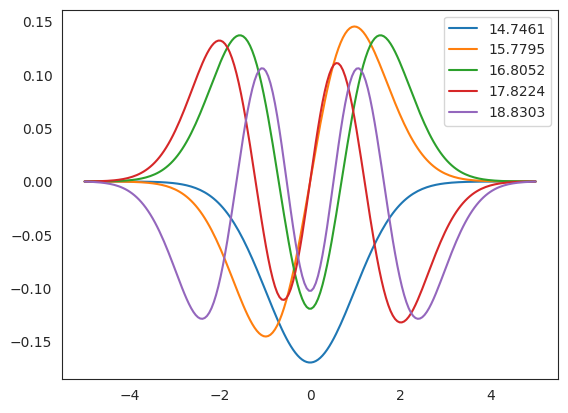
\includegraphics[width=0.9\linewidth]{fig/ks_dft_1d_wfn_ener.png}
  \caption{Wavefunction และพลังงานที่ได้จากการคำนวณ Kohn-Sham DFT สำหรับกรณี 1 มิติ}
  \label{fig:ks_dft_1d_wfn_ener}
\end{figure}

ผู้อ่านที่ต้องการศึกษาโค้ดฉบับสมบูรณ์สามารถดูได้ที่ไฟล์ \ih{6_1D_DFT.ipynb} ใน Code Repository ของหนังสือ \enquote{ปัญญาประดิษฐ์สำหรับเคมีควอนตัม (Machine Learning for Quantum Chemistry)} ที่ \url{https://github.com/rangsimanketkaew/ml-qm-book-code}

%----------------------------------------
\section{เขียนโปรแกรมคำนวณ Molecular Quantum Integrals }
%----------------------------------------

ในเคมีควอนตัมนั้นเราจะต้องปวดหัววุ่นวายกับการคำนวณอินทิกรัล (Integrals) ที่ถือว่าเป็นหนามยอกอกของนักเคมีเชิงฟิสิกส์สายทฤษฎีมาอย่างยาวนาน นั่นก็คือ Molecular Integrals ที่ใช้ Gaussian Basis Functions ซึ่ง Integrals เทอมที่สำคัญ ๆ นั้นก็มีด้วยกันดังนี้
%
\begin{enumerate}[topsep=0pt,noitemsep]
  \setlength\itemsep{0.5em}
  \item Overlap Integrals

  \item Kinetic Energy Integrals

  \item Nuclear Attraction Integrals

  \item Two-Electron Repulsion Integrals
\end{enumerate}
%
โดยในหัวข้อนี้ผู้อ่านจะได้เรียนรู้ทั้งทฤษฎี, อัลกอริทึม และการเขียนโปรแกรมเพื่อคำนวณเทอม Molecular Integrals ทั้ง 4 เทอม

%----------------------------------------
\subsection{ความรู้ทางคณิตศาสตร์ที่ต้องใช้}
%----------------------------------------

เริ่มต้นผมอยากจะให้ผู้อ่านได้ทำความเข้าใจคณิตศาสตร์ที่ควรจะต้องทราบก่อนที่จะไปทำความเข้าใจรายละเอียดของ Integrals โดยผมขอเริ่มด้วย
Gaussian Function แบบสามมิติ ดังนี้
%
\begin{equation}
  G_{ijk}(\mathbf{r}, \alpha, \mathbf{A})
  =
  x_A^i y_A^j z_A^k \hbox{exp}(-\alpha r_A^2)
\end{equation}
%
ซึ่งเป็นฟังก์ชันที่ขึ้นกับพารามิเตอร์ดังต่อไปนี้: Orbital Exponent $\alpha$, Electronic Coordinates $\mathbf{r}$, Origin $\mathbf{A}$, และ
%
\begin{equation}
  \mathbf{r}_A
  =
  \mathbf{r} - \mathbf{A}
\end{equation}
%
แล้วก็ $i,j,k$ คือเลขควอนตัมเชิงมุม (Angular Quantum Numbers) เช่น $i=0$ คือ $s$-type, $i=1$ คือ $p$-type

เนื่องจากว่า Cartesian Gaussians เป็นฟังก์ชันที่ขึ้นกับทิศทาง $,x ,y, z$ ดังนั้นจึงสามารถแยกฟังก์ชันออกจากกันได้ ดังนี้
%
\begin{equation}
  G_{ijk}(\mathbf{r}, \alpha, \mathbf{A})
  =
  G_i(x,\alpha,A_x)G_j(y,\alpha,A_y)G_k(z,\alpha,A_z)
\end{equation}
%
โดยที่ฟังก์ชัน Gaussian แบบหนึ่งมิตินั้นมีสมการคือ
%
\begin{equation}
  G_i(x,\alpha,A_x)
  =
  (x - A_x)^i \hbox{exp}(-\alpha(x-A_x)^2)
\end{equation}

คราวนี้เรามาดู Overlap Integral ของฟังก์ชัน Gaussian แบบหนึ่งมิติ จำนวน 2 ฟังก์ชันกันครับ นั่นคือ $a$ and $b$ ดังนี้
%
\begin{tcolorbox}[ams align]
  S_{ab}
  &= \int G_i(x,\alpha,A_x) G_j(x,\beta,B_x) dx \\
  &= \int K_{AB} x^i_A x^j_B \hbox{exp}(-p x_P^2) dx
\end{tcolorbox}
%
โดยที่เราสามารถใช้คุณสมบัติการคูณของฟังก์ชัน Gaussian ได้ ดังนี้
%
\begin{equation}
  K_{AB}
  =
  \hbox{exp}(-q Q_x^2)
\end{equation}
%
ซึ่ง $q$ และ $Q$ นั้นมีนิยามดังนี้
%
\begin{align}
  Q_x & = A_x - B_x \quad q = \frac{\alpha\beta}{\alpha + \beta}                           \\
  p   & = \alpha + \beta \quad  \quad P_x = \frac{1}{p}\left(\alpha A_x + \beta B_x\right)
\end{align}
%
ถ้าหากว่าเราใช้ฟังก์ชัน Hermite Gaussians เราจะสามารถเขียน $S_{ab}$ ได้ใหม่ดังนี้
%
\begin{align}
  S_{ab}
   & = \int \sum\limits_{t=0}^{i+j} E_{t}^{ij} \Lambda_t dx                \\
   & = \sum\limits_{t=0}^{i+j} E_{t}^{ij} \int \Lambda_t dx                \\
   & = \sum\limits_{t=0}^{i+j} E_{t}^{ij} \delta_{t0} \sqrt{\frac{\pi}{p}} \\
   & = E_{0}^{ij} \sqrt{\frac{\pi}{p}}
\end{align}
%
จะเห็นว่าเราสามารถลดรูปของ Overlap Matrix $S_{ab}$ ให้ง่ายขึ้นได้โดยการใช้คุณสมบัติของ Summation และ Integral แล้วเราก็ยังสามารถทำให้ Summation หายไปได้โดยการยุบรวม $\sum\limits_{t=0}^{i+j} E_{t}^{ij} \delta_{t0}$ เข้าด้วยกัน แล้วเราก็มี $E_{t}^{ij}$ ซึ่งก็คือสัมประสิทธิ์การกระจาย (Expansion Coefficients) ซึ่งเราสามารถคำนวณได้โดยใช้วิธีการวนซ้ำ และ $\Lambda_t$ คือฟัง Hermite Gaussian Overlap ระหว่างฟังก์ชัน Gaussians $a$ กับ $b$ สำหรับการคำนวณหา $E_{t}^{ij}$ เราสามารถใช้สมการต่อไปนี้
%
\begin{subequations}
  \begin{tcolorbox}[ams align]
    E^{ij}_t
    &= \frac{1}{2p}E^{i,j-1}_{t-1} + \frac{qQ_x}{\beta} E_{t}^{i,j-1} + (t+1) E_{t+1}^{i,j-1}
    \label{eq:expan_coeff_1} \\
    E^{ij}_t &= \frac{1}{2p}E^{i-1,j}_{t-1} - \frac{qQ_x}{\alpha} E_{t}^{i-1,j} + (t+1) E_{t+1}^{i-1,j}
    \label{eq:expan_coeff_2}
  \end{tcolorbox}
\end{subequations}
%
โดยสมการที่ \eqref{eq:expan_coeff_1} นั้นช่วยให้เราสามารถลดค่า Index $j$ และสมการที่ \eqref{eq:expan_coeff_2} นั้นช่วยให้เราลดค่าของ Index $i$ ซึ่งทำให้เราได้สมการที่สั้นมากขึ้นนั่นคือสมการที่ \eqref{eq:expan_coeff_3}

\begin{subequations}
  \begin{tcolorbox}[ams gather]
    E^{00}_{0} = K_{AB} \label{eq:expan_coeff_3} \\
    E^{ij}_t = 0 \quad \hbox{ถ้า} \quad t < 0, \quad \hbox{หรือ} \quad t > i+j \label{eq:expan_coeff_4}
  \end{tcolorbox}
\end{subequations}

สรุปก็คือค่าของ $E_{t}^{ij}$ นั้นจะขึ้นอยู่กับค่าของดัชนี $i$, $j$, และ $t$ เช่น ถ้าหากว่า $i = j = t = 0$ เราก็จะได้ Expansion
Coefficient ตามสมการที่ \eqref{eq:expan_coeff_4} นั่นเอง

%----------------------------------------
\subsection{อินทิกรัลซ้อนทับ (Overlap Integrals)}
\idxth{อินทิกรัลซ้อนทับ}
\idxen{Overlap Integrals}
%----------------------------------------

อินทริกรัลอันแรกที่ผู้อ่านจะได้ศึกษาก็คือ Overlap Integrals ซึ่งเราเพิ่งดูรายละเอียดการคำนวณหาอินทิกรัลกันไปในหัวข้อที่แล้วโดยการใช้ Expansion Coefficient $E_t^{ij}$ โดยในหัวข้อนี้เราจะเริ่มด้วยการเขียนฟังก์ชัน \pyinline{E} สำหรับคำนวณ $E_t^{ij}$ ซึ่งนอกจากที่เราจะต้องรู้ค่าของ Angular Momentum $i$ และ $j$ จากฟังก์ชัน Gaussian แล้ว เรายังจะต้องรู้ค่าของระยะห่างระหว่าง Gaussian Function $Q_x$ ด้วย รวมถึงค่าของ Orbital Exponent Coefficients $\alpha$ กับ $\beta$

\vspace{5pt}

\begin{lstlisting}[style=MyPython]
def E(i, j, t, Qx, a, b):
    """
    Recursive definition of Hermite Gaussian coefficients.

    Returns a float.
    a: orbital exponent on Gaussian 'a' (e.g. alpha in the text)
    b: orbital exponent on Gaussian 'b' (e.g. beta in the text)
    i,j: orbital angular momentum number on Gaussian 'a' and 'b'
    t: number nodes in Hermite (depends on type of integral,
        e.g. always zero for overlap integrals)
    Qx: distance between origins of Gaussian 'a' and 'b'
    """
    p = a + b
    q = a * b / p
    if (t < 0) or (t > (i + j)):
        # out of bounds for t
        return 0.0
    elif i == j == t == 0:
        # base case
        return np.exp(-q * Qx * Qx)  # K_AB
    elif j == 0:
        # decrement index i
        return (
            (1 / (2 * p)) * E(i - 1, j, t - 1, Qx, a, b)
            - (q * Qx / a) * E(i - 1, j, t, Qx, a, b)
            + (t + 1) * E(i - 1, j, t + 1, Qx, a, b)
        )
    else:
        # decrement index j
        return (
            (1 / (2 * p)) * E(i, j - 1, t - 1, Qx, a, b)
            + (q * Qx / b) * E(i, j - 1, t, Qx, a, b)
            + (t + 1) * E(i, j - 1, t + 1, Qx, a, b)
        )
\end{lstlisting}

\vspace{5pt}

จะเห็นว่าสำหรับ Overlap แบบหนึ่งมิติ (1D) ระหว่าง Gaussian Function 2 อันนั้น เราก็แค่ทำการคำนวณ $E_0^{ij}$ แล้วก็คูณด้วย $\sqrt{\frac{\pi}{p}}$ แล้วก็ถ้าเป็นแบบสามมิติ (3D) เราก็แค่นำ Overlap แบบ 1D สำหรับ $x,y,z$ มาคูณเข้าด้วยกัน ดังนั้น เราสามารถเขียนโค้ดสำหรับการคำนวณ 3D Overlap ได้ดังนี้

\vspace{5pt}

\begin{lstlisting}[style=MyPython]
import numpy as np


def overlap(a, lmn1, A, b, lmn2, B):
    """
    Evaluates overlap integral between two Gaussians

    Returns a float.
    a: orbital exponent on Gaussian 'a' (e.g. alpha in the text)
    b: orbital exponent on Gaussian 'b' (e.g. beta in the text)
    lmn1: int tuple containing orbital angular momentum (e.g. (1,0,0))
          for Gaussian 'a'
    lmn2: int tuple containing orbital angular momentum for Gaussian 'b'
    A: list containing origin of Gaussian 'a', e.g. [1.0, 2.0, 0.0]
    B: list containing origin of Gaussian 'b'
    """
    l1, m1, n1 = lmn1  # shell angular momentum on Gaussian 'a'
    l2, m2, n2 = lmn2  # shell angular momentum on Gaussian 'b'
    S1 = E(l1, l2, 0, A[0] - B[0], a, b)  # X
    S2 = E(m1, m2, 0, A[1] - B[1], a, b)  # Y
    S3 = E(n1, n2, 0, A[2] - B[2], a, b)  # Z

    return S1 * S2 * S3 * np.power(np.pi / (a + b), 1.5)
\end{lstlisting}

\vspace{5pt}

เราใช้ไลบรารี่ NumPy เพื่อที่ว่าเราสามารถใช้ค่าคงที่ของ $\pi$ และเลขกกำลังแบบเศษส่วน $(3/2)$ ได้นั่นเอง แล้วก็การเขียนฟังก์ชันด้านบน \pyinline{overlap} และ \pyinline{E} ทั้งสองอันนั้นก็เพียงพอแล้วต่อการคำนวณหา Overlap Integrals ระหว่าง Gaussian Function แบบที่เป็น Primitive แต่ประเด็นก็คือว่า Basis Functions ส่วนใหญ่ในการคำนวณทางควอนตัมนั้นเป็นแบบ Contracted Basis Functions นั่นก็คือเป็น Basis Function ที่เกิดจากการรวมเอา Gaussian Primitive Function หลาย ๆ อันมารวมกัน ซึ่งจริง ๆ ถ้าหากว่าเราจะต้องหา Overlap Integrals ระหว่าง Contracted Gaussian Function นั้นก็ทำได้ไม่ยาก โดยสามารถดูได้ในฟังก์ชัน \pyinline{S(a,b)} ดังนี้

\vspace{5pt}

\begin{lstlisting}[style=MyPython]
def S(a, b):
    """
    Evaluates overlap between two contracted Gaussians

    Returns float.
    Arguments:
    a: contracted Gaussian 'a', BasisFunction object
    b: contracted Gaussian 'b', BasisFunction object
    """
    s = 0.0
    for ia, ca in enumerate(a.coefs):
        for ib, cb in enumerate(b.coefs):
            s += (
                a.norm[ia]
                * b.norm[ib]
                * ca
                * cb
                * overlap(a.exps[ia], a.shell, a.origin, b.exps[ib], b.shell, b.origin)
            )

    return s
\end{lstlisting}

\vspace{5pt}

เมื่อเราได้ฟังก์ชัน \pyinline{S(a,b)} แล้ว สิ่งที่เราจะทำต่อไปก็คือเราจะมาลองทดสอบคำนวณค่าของ $S$ กันครับ โดยเราจะลองคำนวณหา $S$ ของ Basis Function 2 อันที่เหมือนกัน ซึ่งคำตอบที่เราจะต้องได้ออกมานั้นแน่นอนว่าจะต้องเท่ากับ 1 เพราะว่าฟังก์ชันที่เหมือนกันก็จะ Overlap กันได้พอดี โดยเราจะต้องมาเขียนโค้ดสำหรับสร้าง Basis Function กันก่อน โดยเราจะใช้ \pyinline{class} สำหรับ \pyinline{BasisFunction} แล้วเราก็จะใช้ \pyinline{class} ดังกล่าวในการสร้าง Object ที่จะมีข้อมูลของ  Basis Function เป็นจำนวนหลาย ๆ อัน โดยโค้ดที่เราจะเขียนนั้นจะอ้างอิงตามสมการต่อไปนี้\footnote{ดูรายละเอียดการพิสูจน์ได้ที่ Fundamentals of Molecular Integrals Evaluation โดย Justin T. Fermann และ Edward F. Valeev\autocite{fermann2020}}

เริ่มด้วย Self-Overlap Integral คือ
%
\begin{equation}
  \int \phi^*(\mathbf{r}) \phi(\mathbf{r}) d \mathbf{r}
  =
  \frac{N^2 \pi^{3 / 2}(2 l-1) ! !(2 m-1) ! !(2 n-1) ! !}{2^{l+m+n}}
  \sum_{i, j}^n \frac{a_i a_j}{\left(\alpha_i+\alpha_j\right)^{l+m+n+3 / 2}}
\end{equation}
%
เนื่องจากว่า $l + m + n = L$ (โมเมนตัมเชิงมุมของแต่ละชั้น (Shell)) เราจะสามารถปรับสมการเพื่อคำนวณหา Normalization
Factor $N$ ได้ดังนี้
%
\begin{align}
  \int \phi^* \phi
   & =
  \frac{N^2 \pi^{3 / 2}(2 l-1) ! !(2 m-1) ! !(2 n-1) ! !}{2^L}
  \sum_{i, j}^n \frac{a_i a_j}{\left(\alpha_i+\alpha_j\right)^{L+3 / 2}} \\
   & =
  1
\end{align}
%
\begin{equation}
  N
  =
  \left[
    \frac{\pi^{3 / 2}(2 l-1) ! !(2 m-1) ! !(2 n-1) ! !}{2^L}
    \sum_{i, j}^n \frac{a_i a_j}{\left(\alpha_i+\alpha_j\right)^{L+3 / 2}}
    \right]^{-1 / 2}
\end{equation}
%
แล้วเราก็จะสามารถเขียนโค้ดเพื่อ Implement สมการที่ ได้ดังนี้

\vspace{5pt}

\begin{lstlisting}[style=MyPython]
from scipy.special import factorial2 as fact2


class BasisFunction(object):
    """
    A class that contains all our basis function data

    Attributes:
    origin: array/list containing the coordinates of the Gaussian origin
    shell: tuple of angular momentum
    exps: list of primitive Gaussian exponents
    coefs: list of primitive Gaussian coefficients
    norm: list of normalization factors for Gaussian primitives
    """

    def __init__(self, origin=[0.0, 0.0, 0.0], shell=(0, 0, 0), exps=[], coefs=[]):
        self.origin = np.asarray(origin)
        self.shell = shell
        self.exps = exps
        self.coefs = coefs
        self.norm = None
        self.normalize()

    def normalize(self):
        """
        Routine to normalize the basis functions,
        in case they do not integrate to unity.
        """
        l, m, n = self.shell
        L = l + m + n
        # self.norm is a list of length equal to number primitives
        # normalize primitives first (PGBFs)
        self.norm = np.sqrt(
            np.power(2, 2 * (l + m + n) + 1.5)
            * np.power(self.exps, l + m + n + 1.5)
            / fact2(2 * l - 1)
            / fact2(2 * m - 1)
            / fact2(2 * n - 1)
            / np.power(np.pi, 1.5)
        )

        # now normalize the contracted basis functions (CGBFs)
        # Eq. 1.44 of Valeev integral whitepaper
        prefactor = (
            np.power(np.pi, 1.5)
            * fact2(2 * l - 1)
            * fact2(2 * m - 1)
            * fact2(2 * n - 1)
            / np.power(2.0, L)
        )

        N = 0.0
        num_exps = len(self.exps)
        for ia in range(num_exps):
            for ib in range(num_exps):
                N += (
                    self.norm[ia]
                    * self.norm[ib]
                    * self.coefs[ia]
                    * self.coefs[ib]
                    / np.power(self.exps[ia] + self.exps[ib], L + 1.5)
                )

        N *= prefactor
        N = np.power(N, -0.5)
        for ia in range(num_exps):
            self.coefs[ia] *= N
\end{lstlisting}

\vspace{5pt}

ถ้าหากว่าเรามี Basis Function STO-3G ของออร์บิทัล $1s$ ของไฮโดรเจนที่มีจุดกำเนิดอยู่ที่ $(1.0, 2.0, 3.0)$ เราจะสามารถสร้าง Basis Function ได้ดังนี้

\vspace{5pt}

\begin{lstlisting}[style=MyPython]
myOrigin = [1.0, 2.0, 3.0]
myShell = (0, 0, 0)  # p-orbitals would be (1,0,0) or (0,1,0) or (0,0,1), etc.
myExps = [3.42525091, 0.62391373, 0.16885540]
myCoefs = [0.15432897, 0.53532814, 0.44463454]
a = BasisFunction(origin=myOrigin, shell=myShell, exps=myExps, coefs=myCoefs)
\end{lstlisting}

\vspace{5pt}

\noindent โดยข้อมูลของ Basis Function ด้านบนนั้นสามารถดูได้จาก STO-3G ของ EMSL Basis Set Exchange Library ดังนี้

\vspace{5pt}

\begin{lstlisting}
!  STO-3G  EMSL  Basis Set Exchange Library 
! Elements                             References
! --------                             ----------
!  H - Ne: W.J. Hehre, R.F. Stewart and J.A. Pople, J. Chem. Phys. 2657 (1969).

****
H     0 
S   3   1.00
      3.42525091             0.15432897       
      0.62391373             0.53532814       
      0.16885540             0.44463454       
****
\end{lstlisting}

\vspace{5pt}

ดังนั้น $S(a,a) = 1.0$ เนื่องจากว่าการ Overlap ของ Basis Function กับตัวมันเองนั้นมีค่าเท่ากับ 1 เพราะว่าเราได้มีการใช้ Normalized Factor $N$ ด้วยนั่นเอง

%----------------------------------------
\subsection{อินทิกรัลพลังงานจลน์ (Kinetic Energy Integrals)}
\idxth{อินทิกรัลพลังงานจลน์}
\idxen{Kinetic Energy Integrals}
%----------------------------------------

เรามาต่อกันที่อินทิกรัลอันที่สองนั่นก็คือ อินทิกรัลพลังงานจลน์ (Kinetic Energy Integrals) ซึ่งสามารถเขียนได้ในรูปของอินทิกรัลซ้อนทับ (Overlap Integral) ดังนี้\footnote{นั่นจึงเป็นเหตุผลที่ว่าทำไมเราถึงต้องดูรายละเอียดของ Overlap Integral เป็นอันดับแรก เพราะว่าเป็นอินทิกรัลสำคัญที่เรานำไปใช้ในการคำนวณอินทิกรัลหรือเทอมอื่น ๆ ในวิชาโครงสร้างเชิงอิเล็กทรอนิกส์}
%
\begin{equation}
  T_{ab}
  =
  -\frac{1}{2}\left[P_{ij}^2 S_{kl} S_{mn} + S_{ij}P_{kl}^2 S_{mn} + S_{ij} S_{kl} P_{mn}^2\right]
\end{equation}
%
โดยที่
%
\begin{equation}
  D_{ij}^2
  =
  j(j-1)S_{i,j-2} - 2\beta(2j +1)S_{ij} + 4\beta^2 S_{i,j+2}
\end{equation}

สำหรับ Primitive Function แบบ 3D เราสามารถสร้างฟังก์ชันสำหรับคำนวณ Kinetic Integral ได้คล้าย ๆ กันกับฟังก์ชันของ Overlap Integral ดังนี้

\vspace{5pt}

\begin{lstlisting}[style=MyPython]
def kinetic(a, lmn1, A, b, lmn2, B):
    """
    Evaluates kinetic energy integral between two Gaussians

    Returns a float.
    a: orbital exponent on Gaussian 'a' (e.g. alpha in the text)
    b: orbital exponent on Gaussian 'b' (e.g. beta in the text)
    lmn1: int tuple containing orbital angular momentum (e.g. (1,0,0))
          for Gaussian 'a'
    lmn2: int tuple containing orbital angular momentum for Gaussian 'b'
    A: list containing origin of Gaussian 'a', e.g. [1.0, 2.0, 0.0]
    B: list containing origin of Gaussian 'b'
    """
    l1, m1, n1 = lmn1
    l2, m2, n2 = lmn2
    term0 = (
        b * (2 * (l2 + m2 + n2) + 3) * overlap(a, (l1, m1, n1), A, b, (l2, m2, n2), B)
    )
    term1 = (
        -2
        * np.power(b, 2)
        * (
            overlap(a, (l1, m1, n1), A, b, (l2 + 2, m2, n2), B)
            + overlap(a, (l1, m1, n1), A, b, (l2, m2 + 2, n2), B)
            + overlap(a, (l1, m1, n1), A, b, (l2, m2, n2 + 2), B)
        )
    )
    term2 = -0.5 * (
        l2 * (l2 - 1) * overlap(a, (l1, m1, n1), A, b, (l2 - 2, m2, n2), B)
        + m2 * (m2 - 1) * overlap(a, (l1, m1, n1), A, b, (l2, m2 - 2, n2), B)
        + n2 * (n2 - 1) * overlap(a, (l1, m1, n1), A, b, (l2, m2, n2 - 2), B)
    )
    return term0 + term1 + term2
\end{lstlisting}

\vspace{5pt}

\noindent และสำหรับ Contracted Gaussian Functions เราสามารถเขียนฟังก์ชัน \pyinline{T(a,b)} ได้ดังนี้

\vspace{5pt}

\begin{lstlisting}[style=MyPython]
def T(a, b):
    """
    Evaluates kinetic energy between two contracted Gaussians

    Returns float.
    Arguments:
    a: contracted Gaussian 'a', BasisFunction object
    b: contracted Gaussian 'b', BasisFunction object
    """
    t = 0.0
    for ia, ca in enumerate(a.coefs):
        for ib, cb in enumerate(b.coefs):
            t += (
                a.norm[ia]
                * b.norm[ib]
                * ca
                * cb
                * kinetic(a.exps[ia], a.shell, a.origin, b.exps[ib], b.shell, b.origin)
            )
    return t
\end{lstlisting}

%----------------------------------------
\subsection{อินทิกรัลแรงดึงดูดเชิงนิวเคลียร์ (Nuclear Attraction Integrals)}
\idxth{อินทิกรัลแรงดึงดูดเชิงนิวเคลียร์}
\idxen{Nuclear Attraction Integrals}
%----------------------------------------

ในหัวข้อนี้เราจะมาดูรายละเอียดของอินทิกรัลอีกอันหนึ่งซึ่งเป็น One-Body Integral นั่นคืออินทิกรัลแรงดึงดูดเชิงนิวเคลียร์ (Nuclear Attraction Integrals) โดยอินทิกรัลอันนี้จะแตกต่างจาก Overlap Integral และ Kinetic Integral ตรงที่เรามีการใช้โอเปอร์เรเตอร์ $1/r_C$ ซึ่งก็คือคูลอมป์ นั่นหมายความว่าเราไม่สามารถทำการแยกตัวประกอบ (Factorization) อินทิกรัลของเราให้อยู่ในรูปของพิกัดคาร์ทีเซียน (Cartesian Components) หรือ $x,y,z$ ได้นั่นเอง ดังนั้นในการคำนวณ Nuclear Attraction Integral เราจำเป็นต้องใช้ตัวช่วยนั่นก็คือ Hermite Coulomb Integral $(R^n_{tuv}(p,\mathbf{P},\mathbf{C}))$ ซึ่งเป็นตัวแทนของอันตรกิริยาแบบคูลอมป์ (Coulomb Interaction) ที่เกิดขึ้นระหว่างการกระจายตัวของประจุแบบ Gaussian ในโมเลกุลซึ่งมีจุดศูนย์กลางคือ $\mathbf{P}$ ส่วนนิวเคลียสนั้นมีจุดศูนย์กลางอยู่ที่ $\mathbf{C}$ โดย Hermite Coulomb Integral นั้นมีองค์ประกอบคือ $E_t^{ij}$ ซึ่งสามารถหาได้ด้วยวิธีการวนซ้ำตามชุดสมการดังต่อไปนี้
%
\begin{align}
  R^{n}_{t+1,u,v} & = t R^{n+1}_{t-1,u,v} + X_{PC}R^{n+1}_{t,u,v} \\
  R^{n}_{t,u+1,v} & = u R^{n+1}_{t,u-1,v} + Y_{PC}R^{n+1}_{t,u,v} \\
  R^{n}_{t,u,v+1} & = v R^{n+1}_{t,u,v-1} + Z_{PC}R^{n+1}_{t,u,v} \\
  R^{n}_{0,0,0}   & = (-2p)^n F_n (p R_{PC}^2)
\end{align}
%
โดยที่ $F_n(T)$ คือฟังก์ชันของบอยส์ (Boys Function)
%
\begin{equation}
  F_n(T)
  =
  \int_0^1 \hbox{exp}(-Tx^2)x^{2n}dx
\end{equation}
%
ซึ่ง Boys Function นั้นเป็นกรณีเฉพาะแบบพิเศษของ Kummer Confluent Hypergeometric Function $_1F_1(a,b,x)$ ดังนี้\footnote{\url{https://en.wikipedia.org/wiki/Confluent_hypergeometric_function}}
%
\begin{equation}
  F_n(T)
  =
  \frac{_1F_1(n+\frac{1}{2}, n+\frac{3}{2}, -T)}{2n+1}
\end{equation}
%
โดยที่เราสามารถ Implement สมการด้านบนนี้ได้ง่าย ๆ โดยการใช้ฟังก์ชันของไลบรารี่ \pyinline{SciPy} สำหรับ $_1F_1$ ซึ่งอยู่ในโมดูล \pyinline{scipy.special}

\vspace{5pt}

\begin{lstlisting}[style=MyPython]
def R(t, u, v, n, p, PCx, PCy, PCz, RPC):
    """
    Returns the Coulomb auxiliary Hermite integrals

    Returns a float.
    Arguments:
    t,u,v: order of Coulomb Hermite derivative in x,y,z
           (see defs in Helgaker and Taylor)
    n: order of Boys function
    PCx,y,z: Cartesian vector distance between Gaussian
             composite center P and nuclear center C
    RPC: Distance between P and C
    """
    T = p * RPC * RPC
    val = 0.0
    if t == u == v == 0:
        val += np.power(-2 * p, n) * boys(n, T)
    elif t == u == 0:
        if v > 1:
            val += (v - 1) * R(t, u, v - 2, n + 1, p, PCx, PCy, PCz, RPC)
        val += PCz * R(t, u, v - 1, n + 1, p, PCx, PCy, PCz, RPC)
    elif t == 0:
        if u > 1:
            val += (u - 1) * R(t, u - 2, v, n + 1, p, PCx, PCy, PCz, RPC)
        val += PCy * R(t, u - 1, v, n + 1, p, PCx, PCy, PCz, RPC)
    else:
        if t > 1:
            val += (t - 1) * R(t - 2, u, v, n + 1, p, PCx, PCy, PCz, RPC)
        val += PCx * R(t - 1, u, v, n + 1, p, PCx, PCy, PCz, RPC)
    return val
\end{lstlisting}

\vspace{5pt}

\noindent และเราสามารถทำการกำหนด Boys Function โดยการเขียนฟังก์ชัน \pyinline{boys(n,T)} ได้ดังนี้

\vspace{5pt}

\begin{lstlisting}[style=MyPython]
from scipy.special import hyp1f1

def boys(n, T):
    return hyp1f1(n + 0.5, n + 1.5, -T) / (2.0 * n + 1.0)
\end{lstlisting}

\vspace{5pt}

\noindent แล้วเราก็สามารถคำนวณ $\mathbf{P}$ ได้โดยการใช้ Gaussian Product Center Rule ดังนี้
%
\begin{equation}
  P
  =
  \frac{\alpha A + \beta B}{\alpha + \beta}
\end{equation}

\noindent ซึ่งสามารถเขียนออกมาเป็นโค้ดได้ง่าย ๆ ดังนี้

\vspace{5pt}

\begin{lstlisting}[style=MyPython]
def gaussian_product_center(a, A, b, B):
    return (a * A + b * B) / (a + b)
\end{lstlisting}

\vspace{5pt}

เมื่อเราคำนวณ Coulomb Auxiliary Hermite Integrals $R^{n}_{tuv}$ ออกมาได้แล้ว ขั้นตอนต่อไปคือเราสามารถคำนวณ Nuclear Attraction Integral โดยเทียบกับนิวเคลียสที่มีจุดศูนย์กลางอยู่ที่ $\mathbf{C}$, $V_{ab}(C)$ ได้โดยการใช้สมการต่อไปนี้
%
\begin{equation}
  V_{ab}(C)
  =
  \frac{2\pi}{p}
  \sum\limits_{t,u,v}^{\substack{i+j+1,\\k+l+1,\\m+n+1}}
  E_t^{ij} E_u^{kl} E_v^{mn} R^0_{tuv}(p,\mathbf{P},\mathbf{C})
\end{equation}
%
ซึ่งเราก็จะสามารถ Implement สมการด้านบนนี้ให้เป็นโค้ดตามฟังก์ชัน \pyinline{nuclear_attraction} ได้ดังนี้

\vspace{5pt}

\begin{lstlisting}[style=MyPython]
def nuclear_attraction(a, lmn1, A, b, lmn2, B, C):
    """
    Evaluates kinetic energy integral between two Gaussians

    Returns a float.
    a: orbital exponent on Gaussian 'a' (e.g. alpha in the text)
    b: orbital exponent on Gaussian 'b' (e.g. beta in the text)
    lmn1: int tuple containing orbital angular momentum (e.g. (1,0,0))
          for Gaussian 'a'
    lmn2: int tuple containing orbital angular momentum for Gaussian 'b'
    A: list containing origin of Gaussian 'a', e.g. [1.0, 2.0, 0.0]
    B: list containing origin of Gaussian 'b'
    C: list containing origin of nuclear center 'C'
    """
    l1, m1, n1 = lmn1
    l2, m2, n2 = lmn2
    p = a + b
    P = gaussian_product_center(a, A, b, B)  # Gaussian composite center
    RPC = np.linalg.norm(P - C)

    val = 0.0
    for t in range(l1 + l2 + 1):
        for u in range(m1 + m2 + 1):
            for v in range(n1 + n2 + 1):
                val += (
                    E(l1, l2, t, A[0] - B[0], a, b)
                    * E(m1, m2, u, A[1] - B[1], a, b)
                    * E(n1, n2, v, A[2] - B[2], a, b)
                    * R(t, u, v, 0, p, P[0] - C[0], P[1] - C[1], P[2] - C[2], RPC)
                )
    val *= 2 * np.pi / p
    return val
\end{lstlisting}

\vspace{5pt}

\noindent และเราก็สามารถใช้ Contracted Gaussians ในการคำนวณอินทิกรัลของเราได้ตามที่แสดงในโค้ดดังต่อไปนี้

\vspace{5pt}

\begin{lstlisting}[style=MyPython]
def V(a, b, C):
    """
    Evaluates overlap between two contracted Gaussians

    Returns float.
    Arguments:
    a: contracted Gaussian 'a', BasisFunction object
    b: contracted Gaussian 'b', BasisFunction object
    C: center of nucleus
    """
    v = 0.0
    for ia, ca in enumerate(a.coefs):
        for ib, cb in enumerate(b.coefs):
            v += (
                a.norm[ia]
                * b.norm[ib]
                * ca
                * cb
                * nuclear_attraction(
                    a.exps[ia], a.shell, a.origin, b.exps[ib], b.shell, b.origin, C
                )
            )
    return v
\end{lstlisting}

\vspace{5pt}

ผู้อ่านจะต้องเข้าใจด้วยว่าอินทิกรัลที่เราคำนวณออกมาได้นั้นเป็นแค่ Nuclear Attraction เท่านั้น ซึ่งเรายังมี Nuclear Repulsion Integrals ที่เป็น Contribution มาจากอะตอมที่มีจุดศูนย์กลางอยู่ที่ $\mathbf{C}$ อีกด้วย ถ้าหากว่าเราต้องการคำนวณ Nuclear Attraction Contribution ทั้งหมดของทั้งโมเลกุล เราจะต้องทำการรวม Integral ทั้งหมดทุกเทอมของทุกอะตอมเข้าด้วยแล้วก็ทำตามปรับสเกลของแต่ละ Integral ตามประจุย่อย (Nuclear Charge) ของอะตอมนั้น ๆ

%----------------------------------------
\subsection{อินทิกรัลแรงผลักระหว่างอิเล็กตรอน (Two-Electron Repulsion Integrals)}
\idxth{อินทิกรัลแรงผลักระหว่างอิเล็กตรอน}
\idxen{Two-Electron Repulsion Integrals}
%----------------------------------------

เราได้ศึกษารายละเอียดของ One-Body Integrals ไปแล้ว ซึ่งเป็นอินทิกรัลพื้นฐานที่ผู้อ่านควรจะต้องทราบหากต้องการเขียนโปรแกรมคำนวณพลังงานของโมเลกุลด้วยวิธี Hartree-Fock ในหัวข้อนี้เราจะมาดูรายละเอียดของอินทิกรัลอันสุดท้ายซึ่งเป็นอินทิกรัลที่สำคัญมากและมีความซับซ้อนมากเช่นกัน นั่นคืออินทิกรัลของแรงผลักระหว่างอิเล็กตรอน (Electron-Electron Repulsion Integrals) ซึ่งเป็นอินทิกรัลแบบ Two-Body

ในการคำนวณหาอินทิกรัลอันนี้นั้น เราจะยังคงมีการใช้ Hermite Integrals ซึ่งเราจะต้องทำการหาผลรวมดังต่อไปนี้
%
\begin{equation}
  \begin{aligned}
    g_{abcd}
    =
     & \frac{2\pi^{5/2}}{pq\sqrt{p+q}}              \\
     & \sum\limits_{t,u,v}^{\substack{i+j+1,        \\k+l+1, \\m+n+1}}
    E_t^{ij}
    E_u^{kl}
    E_v^{mn}
    \sum\limits_{\tau,\nu,\phi}^{\substack{i'+j'+1, \\k'+l'+1, \\m'+n'+1}}
    E_{\tau}^{i'j'}
    E_{\nu}^{k'l'}
    E_{\phi}^{m'n'}
    (-1)^{\tau+\nu+\phi}
    R^0_{t+\tau, u + \nu, v+\phi}(p,q,\mathbf{P},\mathbf{Q})
  \end{aligned}
\end{equation}
%
ซึ่งจะเห็นได้ว่าสมการด้านบนนี้น่ากลัวมาก มีความซับซ้อนมาก อย่างไรก็ตาม เนื่องจากว่าเราทราบว่า $p = \alpha + \beta$ เราจะกำหนดให้ $q = \gamma + \delta$ เพื่อที่ว่าเราจะได้มี Gaussian Function Exponents ของ $a$, $b$, $c$ และ $d$ ซึ่งเราสามารถเขียนสมการใหม่อีกสมการที่มีหน้าตาคล้าย ๆ กับ Nuclear Attraction Integrals ได้ดังนี้

\vspace{5pt}

\begin{lstlisting}[style=MyPython]
def electron_repulsion(a, lmn1, A, b, lmn2, B, c, lmn3, C, d, lmn4, D):
    """
    Evaluates kinetic energy integral between two Gaussians

    Returns a float.
    a,b,c,d: orbital exponent on Gaussian 'a','b','c','d'
    lmn1,lmn2
    lmn3,lmn4: int tuple containing orbital angular momentum
               for Gaussian 'a','b','c','d', respectively
    A,B,C,D: list containing origin of Gaussian 'a','b','c','d'
    """
    l1, m1, n1 = lmn1
    l2, m2, n2 = lmn2
    l3, m3, n3 = lmn3
    l4, m4, n4 = lmn4
    p = a + b  # composite exponent for P (from Gaussians 'a' and 'b')
    q = c + d  # composite exponent for Q (from Gaussians 'c' and 'd')
    alpha = p * q / (p + q)
    P = gaussian_product_center(a, A, b, B)  # A and B composite center
    Q = gaussian_product_center(c, C, d, D)  # C and D composite center
    RPQ = np.linalg.norm(P - Q)

    val = 0.0
    for t in range(l1 + l2 + 1):
        for u in range(m1 + m2 + 1):
            for v in range(n1 + n2 + 1):
                for tau in range(l3 + l4 + 1):
                    for nu in range(m3 + m4 + 1):
                        for phi in range(n3 + n4 + 1):
                            val += (
                                E(l1, l2, t, A[0] - B[0], a, b)
                                * E(m1, m2, u, A[1] - B[1], a, b)
                                * E(n1, n2, v, A[2] - B[2], a, b)
                                * E(l3, l4, tau, C[0] - D[0], c, d)
                                * E(m3, m4, nu, C[1] - D[1], c, d)
                                * E(n3, n4, phi, C[2] - D[2], c, d)
                                * np.power(-1, tau + nu + phi)
                                * R(
                                    t + tau,
                                    u + nu,
                                    v + phi,
                                    0,
                                    alpha,
                                    P[0] - Q[0],
                                    P[1] - Q[1],
                                    P[2] - Q[2],
                                    RPQ,
                                )
                            )

    val *= 2 * np.power(np.pi, 2.5) / (p * q * np.sqrt(p + q))
    return val
\end{lstlisting}

\vspace{5pt}

\noindent และเพื่อให้มีความสมบูรณ์มากกว่านี้ เราจะสามารถเขียนฟังก์ชันเพื่อคำนวณหา Electron-Electron Respulsion Integral สำหรับ Contracted Gaussians ได้ดังนี้

\vspace{5pt}

\begin{lstlisting}[style=MyPython]
def ERI(a, b, c, d):
    """
    Evaluates overlap between two contracted Gaussians

    Returns float.
    Arguments:
    a: contracted Gaussian 'a', BasisFunction object
    b: contracted Gaussian 'b', BasisFunction object
    c: contracted Gaussian 'b', BasisFunction object
    d: contracted Gaussian 'b', BasisFunction object
    """
    eri = 0.0
    for ja, ca in enumerate(a.coefs):
        for jb, cb in enumerate(b.coefs):
            for jc, cc in enumerate(c.coefs):
                for jd, cd in enumerate(d.coefs):
                    eri += (
                        a.norm[ja]
                        * b.norm[jb]
                        * c.norm[jc]
                        * d.norm[jd]
                        * ca
                        * cb
                        * cc
                        * cd
                        * electron_repulsion(
                            a.exps[ja],
                            a.shell,
                            a.origin,
                            b.exps[jb],
                            b.shell,
                            b.origin,
                            c.exps[jc],
                            c.shell,
                            c.origin,
                            d.exps[jd],
                            d.shell,
                            d.origin,
                        )
                    )
    return eri
\end{lstlisting}

\vspace{5pt}

ทั้งหมดที่เราเพิ่งดูรายละเอียดกันไปนั้นคือสมการและการเขียนโค้ดของอินทิกรัลทั้งหมดที่จำเป็นต้องใช้ในการเขียนโปรแกรมเคมีควอนตัมด้วยวิธี Hartree-Fock นั่นเองครับ

%----------------------------------------
\subsection{การพิจารณาประสิทธิภาพเชิงการคำนวณ (Computational Efficiency)}
%----------------------------------------

ในหัวข้อก่อนหน้านี้ที่เราได้ศึกษา Integrals แบบต่าง ๆ กันไปแล้ว ทั้งสมการคณิตศาสตร์และการเขียนโปรแกรม ผู้อ่านจะพบว่าโค้ดที่ผมเอามาให้ดูเป็นตัวอย่างนั้นสามารถทำงานได้ตามปกติ ให้ผลการคำนวณที่ถูกต้อง แต่ประเด็นสำคัญอีกอย่างหนึ่งก็คือประสิทธิภาพของโค้ดที่เขียนขึ้นมา แน่นอนว่าโค้ดของเรารันได้ แต่ว่าจะโค้ดจะทำงานได้ช้าหรือเร็วนั้นก็ขึ้นอยู่กับว่าเราเขียนโค้ดอย่างไร นอกจากนี้ยังขึ้นกับภาษาที่เราใช้ในการเขียนด้วย โดยภาษาที่ผมเลือกมาใช้ในการเขียนโค้ดในหนังสือเล่มนี้นั้นส่วนใหญ่เป็นภาษา Python เพราะว่าเขียนได้ง่าย ถึงแม้ว่าโค้ดที่เขียนด้วยภาษา Python นั้นจะทำงานได้ช้ากว่าโค้ดที่เขียนด้วยภาษาอื่น แต่ Python นั้นสามารถศึกษาตามได้ง่ายกว่ามาก ๆ

ถ้าหากว่าเราเขียนโค้ดออกมาแล้วนำไปรันทันทีเลยโดยที่ไม่มีพิจารณาประสิทธิภาพเชิงการคำนวณก่อน โค้ดของเราก็อาจจะไม่สามารถทำงานบนคอมพิวเตอร์ที่มีประสิทธิภาพสูง เช่น Supercomputer ได้อย่างเต็มที่ ดังนั้นเราจะมาดูกันว่ามีปัจจัยอะไรที่เราจะสามารถศึกษาเพื่อนำมาใช้ในการปรับปรุงโค้ดของเราเพื่อให้มีประสิทธิภาพมากขึ้นในการนำไปใช้งานจริง

ปัจจัยแรกเลยคือภาษาคอมพิวเตอร์ที่เรานำมาใช้ในการเขียนโค้ด จริง ๆ แล้วถ้าหากว่าเราอยากจะเขียนโค้ดแบบจริงจังเพื่อให้ทำงานได้อย่างมีประสิทธิภาพ เราไม่ควรเขียนโปรแกรมโดยการใช้เพียงแค่ภาษา Python เพราะว่าภาษา Python นั้นจะทำงานได้ช้ากว่าภาษาคอมพิวเตอร์อื่นที่เป็นแบบ Low-Level เหตุผลที่โค้ดของเราด้านบนที่ถูกด้วยเขียน Python ทำงานได้ช้านั้นก็เพราะว่าเรามีการวนลูปโดยการใช้ \pyinline{for} แบบหลาย ๆ ชั้น (Nested Loop) ซึ่งเป็นตัวการที่ทำให้โค้ดของเราช้า ดังนั้นจึงจะเป็นการดีกว่าถ้าหากว่าเราเขียนบางส่วนของโค้ด Python ของเราด้วยเทคนิคต่าง ๆ โดยหนึ่งในนั้นก็คือการเขียนโค้ดใหม่ด้วย Cython (\url{http://www.cython.org}) ซึ่งจะช่วยให้โค้ดของเราทำงานได้เร็วขึ้นหลายสิบเท่าเลย ปัญหาอีกอย่างหนึ่งของ Python ก็คือมีการใช้ Global Interpreter Lock (GIL) ซึ่งทำให้เราไม่สามารถรันโค้ดของเราแบบขนาน (Parallel) ได้ ซึ่งถ้าหากว่าเราสามารถทำการแบ่ง Routine ในโค้ดการคำนวณ Integral ของเราออกเป็นหลาย ๆ อันและทำการรัน Routines เหล่านั้นด้วย CPUs หลาย ๆ อันได้ก็จะทำให้โค้ดเราทำงานได้เร็วขึ้นเยอะมาก โดยหนึ่งในวิธีการเขียนโค้ดแบบ Parallel นั้นก็คือการใช้วิธี OpenMP หรือใช้โมดูลของ Cython นั่นคือ \pyinline{cython.parallel} โดยผู้อ่านสามารถนำเทคนิคเหล่านี้ไปใช้ในการทำให้โค้ดการคำนวณ Integrals ของเราได้ เช่น หลีกเลี่ยงการคำนวณแบบวนซ้ำหลาย ๆ รอบ (Explicit Recursion) ในฟังก์ชัน \pyinline{E} และ \pyinline{R}

นอกจากนี้ผู้อ่านยังสามารถใช้เทคนิคอื่น ๆ ได้อีก เช่น ใช้ Permutational Symmetry ของอินทิกรัล เช่น เราสามารถทำการคำนวณ Two-Electron Repulsion Integral ได้เร็วขึ้นประมาณ 8 เท่าเพียงแค่นำคุณสมบัติของความสมมาตรของอินทิกรัลมาใช้ แล้วเราก็สามารถหลักเลี่ยงการคำนวณ Integrals หลาย ๆ อันที่มีค่าเท่ากับศูนย์ได้เพื่อเป็นการประหยัดเวลาในการคำนวณ

%----------------------------------------
\section{การเพิ่มประสิทธิภาพการแปลง Two-Electron Integral}
%----------------------------------------

อัลกอริทึมแบบที่มีประสิทธิภาพในการสเกล (Scaling Performance) ที่ต่ำนั้นทำให้การคำนวณทางเคมีควอนตัมนั้นเสียเวลาและเปลืองทรัพยากร เช่น พลังงาน ตัวอย่างหนึ่งที่เห็นได้ชัดนั่นก็คือการแปลงอินทิกรัล (Integral Transformation) ของเทอม Two-Electron Integral ในโปรแกรมทาง Electronic Structure ซึ่งถ้าหากว่าอัลกอริทึมที่เราใช้นั้นไม่มีประสิทธิภาพ การ Transformation นั้นก็จะมีการสเกลมากถึง $O(N^{8})$ ทำให้การคำนวณของโมเลกุลที่มีขนาดใหญ่นั้นใช้เวลานานมากหรือแทบจะคำนวณไม่ได้เลย ดังนั้นจึงได้มีการปรับปรุงให้การ Transformation นั้นทำได้ง่ายขึ้นโดยเราสามารถลดการสเกลลงมาได้อยู่ในระดับ $O(N^{5})$ เลยทีเดียว

ถ้าหากว่าเราคำนวณ Hartree-Fock (HF) เราจะต้องมีการนำเมทริกซ์ของ Molecular Orbital Coefficients หลาย ๆ อันมาคูณกัน ซึ่ง Coefficients เหล่านี้เป็น Eigenvectors ที่สอดคล้องกับ HF Hamiltonian (Fock Matrix) นั่นเอง ส่วนค่า Eigenvalues นั้นก็เป็นพลังงานของออร์บิทัล โดยเทคนิคที่เราสามารถนำมาใช้ในการลดความซับซ้อนของการคำนวณ Two-Electron Integral ลงได้นั้นก็คือเทคนิค Orbital Transformation ซึ่งเป็นการแปลง Two-Electron Integral จาก Atomic Orbital Basis (ซึ่งก็คือ Basis Functions ที่เรานำมาใช้ในการสร้าง Atomic Orbital) ให้กลายเป็น Molecular Orbital Basis แทน แล้วเราก็ทำการ Project อินทิกรัลที่คำนวณได้ไปบนฟังก์ชันคลื่นของโมเลกุล ซึ่งวิธีที่เราทำเริ่มต้นด้วย
\idxboth{วิธีฮาร์ทรี-ฟ็อค}{Hartree-Fock Method}
%
\begin{equation}
  (pq\vert rs)
  =
  \sum_\mu \sum_\nu \sum_\lambda \sum_\sigma
  C^{p}_\mu C^{q}_\nu C^{r}_\lambda C^{s}_\sigma(\mu\nu\vert \lambda\sigma)
\end{equation}
%
ซึ่งเขียนเป็นโค้ดด้วยภาษา Python โดยการใช้ \pyinline{for} ได้คร่าว ๆ ดังนี้

\vspace{5pt}

\begin{lstlisting}[style=MyPython]
for p in range(0,dim):  
  for q in range(0,dim):  
    for r in range(0,dim):  
      for s in range(0,dim):  
        for mu in range(0,dim):  
          for nu in range(0,dim):  
            for lam in range(0,dim):  
              for sig in range(0,dim):  
                TxInt[p,q,r,s] += C[p,mu]*C[q,nu]*C[r,lam]*C[s,sig]*UnTxInt[mu,nu,lam,sig]
\end{lstlisting}

\vspace{5pt}

\noindent จะเห็นได้ว่าถ้าเรารันโค้ดด้านบนนี้จะใช้เวลานานมาก ๆ เพราะว่าเรามีการวนซ้ำ \pyinline{for} ถึง 8 ชั้นด้วยกัน โดยการสเกลนั้นจะแปรผันตรงตามจำนวนของ Basis Functions ที่เราใช้ยกกำลังด้วย 8 ซึ่งเยอะมาก ๆ

ถ้าหากว่าเราสังเกตสมการด้านบนนี้ดี ๆ จะพบว่า Coefficients แต่ละตัวนั้นไม่ขึ้นต่อกัน เช่น $C^{p}_\mu$ ก็ไม่ขึ้นกับ $C^{q}_\nu$ ดังนั้นเราจึงสามารถเขียนสมการใหม่ได้เป็น
%
\begin{equation}
  (pq\vert rs)
  =
  \sum_\mu C^{p}_\mu
  [\sum_\nu C^{q}_\nu
    [\sum_\lambda C^{r}_\lambda
      [\sum_\sigma C^{s}_\sigma(\mu\nu\vert \lambda\sigma)]]]
\end{equation}
%
หรือถ้าอยากให้เห็นภาพชัด ๆ และเข้าใจมากกว่านี้ก็สามารถเขียนโดยอินทิกรัลแต่ละอันแยกจากกันได้ ดังนี้
%
\begin{gather}
  (\mu\nu\vert \lambda s) = \sum_\sigma C^{s}_\sigma(\mu\nu\vert \lambda\sigma) \\
  (\mu\nu\vert rs) = \sum_\lambda C^{r}_\lambda(\mu\nu\vert \lambda s) \\
  (\mu q\vert rs) = \sum_\nu C^{q}_\nu(\mu\nu\vert rs) \\
  (pq\vert rs) = \sum_\mu C^{p}_\mu(\mu q\vert rs)
\end{gather}
%
นั่นก็คือเราทำการแปลง Quarter Transformation ทั้งหมด 4 อัน โดยเราจะทำการบันทึก Transformation ที่คำนวณเสร็จแล้วเก็บไว้ใช้สำหรับการคำนวณ Transformation อันต่อไป ซึ่งท้ายที่สุดแล้วเราจะสามารถเขียนโค้ดของการแปลงดังกล่าวได้โดยการใช้ Loop เพียงแค่ 5 Loops เท่านั้น ซึ่งนั่นก็คือเป็นการลดสเกลลงเหลือแค่ $N^{5}$ ดังนี้

\vspace{5pt}

\begin{lstlisting}[style=MyPython]
for p in range(0,dim):  
  for mu in range(0,dim):  
    temp[p,:,:,:] += C[p,mu]*UnTXInt[mu,:,:,:]  
  for q in range(0,dim):  
    for nu in range(0,dim):  
      temp2[p,q,:,:] += C[q,nu]*temp[p,nu,:,:]  
    for r in range(0,dim):  
      for lam in range(0,dim):  
        temp3[p,q,r,:] += C[r,lam]*temp2[p,q,lam,:]  
      for s in range(0,dim):  
        for sig in range(0,dim):  
          TxInt[p,q,r,s] += C[s,sig]*temp3[p,q,r,sig]
\end{lstlisting}

\vspace{5pt}

\noindent โดยโค้ดเวอร์ชั่นที่สองนี้เขียนได้ดีกว่าเวอร์ชั่นแรกเยอะมาก นอกจากนี้จะสังเกตได้ว่าเราได้มีการใช้เมทริกซ์ \pyinline{temp} เพื่อใช้ในการเก็บผลลัพธ์ที่ได้ระหว่างการคำนวณ Quarter Transformations แล้วก็ Transformation นั้นก็มีการใช้ Slice Notation ใน Python/Numpy ด้วยซึ่งทำให้เราสามารถทำ Transformation ได้ครบทุก Dimension ของเมทริกซ์ (แทนที่จะใช้ Indices)

ด้านล่างคือโค้ดแบบสมบูรณ์ของการทำ Integral Transformation โดยมีการบันทึกเวลาว่าทั้งสองวิธีนั้นใช้เวลานานแค่ไหนแล้วก็มาเปรียบเทียบกัน

\vspace{5pt}

\begin{lstlisting}[style=MyPython]
import numpy as np
import time

# Dimension of arrays ... e.g number of basis functions
dim = 5
# For our first dumb O[N^8] method
MO1 = np.zeros((dim, dim, dim, dim))  
# For our smarter O[N^5] method
MO2 = np.zeros((dim, dim, dim, dim))  

INT = np.random.randint(
    9, size=(dim, dim, dim, dim)
)  # Our toy "two electron integrals"
# Toy "wavefunction coefficients"
C = np.random.randint(9, size=(dim, dim))  

# First method: N^8

t0 = time.time()
for i in range(0, dim):
    for j in range(0, dim):
        for k in range(0, dim):
            for l in range(0, dim):
                for m in range(0, dim):
                    for n in range(0, dim):
                        for o in range(0, dim):
                            for p in range(0, dim):
                                MO1[i, j, k, l] += (
                                    C[i, m]
                                    * C[j, n]
                                    * C[k, o]
                                    * C[l, p]
                                    * INT[m, n, o, p]
                                )
t1 = time.time()

# Second method: N^5

t2 = time.time()
temp = np.zeros((dim, dim, dim, dim))
temp2 = np.zeros((dim, dim, dim, dim))
temp3 = np.zeros((dim, dim, dim, dim))
for i in range(0, dim):
    for m in range(0, dim):
        temp[i, :, :, :] += C[i, m] * INT[m, :, :, :]
    for j in range(0, dim):
        for n in range(0, dim):
            temp2[i, j, :, :] += C[j, n] * temp[i, n, :, :]
        for k in range(0, dim):
            for o in range(0, dim):
                temp3[i, j, k, :] += C[k, o] * temp2[i, j, o, :]
            for l in range(0, dim):
                for p in range(0, dim):
                    MO2[i, j, k, l] += C[l, p] * temp3[i, j, k, p]
t3 = time.time()

# Set up random index to check correctness.
i = np.random.randint(dim)
j = np.random.randint(dim)
k = np.random.randint(dim)
l = np.random.randint(dim)

print(MO1[i, j, k, l])
print(MO2[i, j, k, l])
print("Time 1: ", t1 - t0)
print("Time 2: ", t3 - t2)
\end{lstlisting}
%
\vspace{5pt}
%
โดยได้เอาต์พุตออกมาดังนี้
%
\vspace{5pt}
%
\begin{lstlisting}
1904496.0
1904496.0
Time 1:  0.2975327968597412
Time 2:  0.0035715103149414062
\end{lstlisting}

\vspace{5pt}

เมื่อเรารันโค้ดแล้วจะพบว่าระยะเวลาที่วิธีที่หนึ่งใช้นั้นจะนานกว่าวิธีที่สองมาก (ผมกำหนดจำนวน Basis Functions = 5) โดยใช้เวลาประมาณ 0.298 และ 0.004 วินาที ตามลำดับ ดังนั้นจึงสรุปได้ว่าวิธีที่สองนั้นมีประสิทธิภาพมากกว่าวิธีแรกในเชิงของการคำนวณอย่างมาก นอกจากนี้เรายังสามารถ Parallel อัลกอริทึมของวิธีที่สองเพื่อให้ทำงานได้เร็วมากยิ่งขึ้นกว่านี้ได้อีกด้วย\footnote{ผมอยากให้ผู้อ่านลองวิเคราะห์ว่าเราจะทำการ Parallel โค้ดของวิธีที่สองได้อย่างไร}

%----------------------------------------
\section{คำแนะนำสำหรับการคำนวณเคมีควอนตัม}
%----------------------------------------

คนที่ทำวิจัยด้านเคมีควอนตัมก็จะมีเทคนิคหรือแนวทางในการทำการคำนวณเคมีควอนตัมของตนเอง ขึ้นอยู่กับหลายปัจจัย ตัวอย่างเช่น เรียนจากคอร์สของมหาวิทยาลัย, อ่านจากหนังสือหรือตำราต่างประเทศที่ต่างกัน, ได้รับคำชี้แนะจากการทำวิจัยจากหลาย ๆ คน รวมถึงประสบการณ์หรือความเคยชินกับโปรแกรมเคมีควอนตัมที่ตนเองถนัด อย่างไรก็ตาม ผมคิดว่าเราทุกคนควรจะต้องมีหลักการทางทฤษฎีที่ถูกต้องที่ควรจะต้องปฏิบัติตามกัน ซึ่งก็คือการเข้าใจทฤษฎีทางเคมีควอนตัมและโครงสร้างเชิงอิเล็กทรอนิกส์ ในหัวข้อนี้ผู้อ่านได้จะศึกษาแนวทางสำหรับการคำนวณเคมีควอนตัม

\paragraph{1. การเตรียม Input File โครงสร้างของโมเลกุลและการเลือก Electronic State}
%
ผมขอเริ่มด้วยสิ่งที่เป็นพื้นฐานที่สุดนั่นก็คือการเตรียมไฟล์อินพุต (Input) ซึ่งปกติแล้วเรามักจะทราบกันดีว่าเราสามารถแสดง (Represent) โครงสร้างของโมเลกุลได้ด้วยรูปแบบ (Format) 2 อัน นั่นคือ Cartesian (xyz) Format กับ Z-Matrix Format โดยใน xyz Format นั้นเราจะใส่ลิสต์รายละเอียดของอะตอมในโมเลกุลนั่นคือเลขอะตอมและพิกัด Cartesian Coordinates ของอะตอมแต่ละตัว ส่วนใน Z-Matrix Format นั้นจะเป็นการกำหนดโครงสร้างหรือ Geometry โดยการใช้พิกัดภายใน (Internal Coordinates) เช่น ควาามยาวพันธะ มุมพันธะ และมุมบิด โดยโปรแกรมควอนตัมเคมีส่วนใหญ่นั้นทำการกำหนดรูปแบบเริ่มต้นของโครงสร้างโมเลกุลเป็นแบบพิกัด Cartesian รวมถึงพารามิเตอร์อื่น ๆ เช่น กำหนดหน่วยเป็น Angstroms แต่ว่าโปรแกรมแต่ละโปรแกรมนั้นก็มักจะมีคีเวิร์ดให้สลับไปใช้หน่วยอื่น เช่น bohr พารามิเตอร์ที่สำคัญอีก 2 อันก็คือ Charge กับ Spin Multiplicity ของ Electronic State ที่เราสนใจที่จะศึกษา โดยประจุนั้นเป็นการระบุถึงจำนวนของอิเล็กตรอน ส่วน Spin Multiplicity หาได้จากจำนวนรูปแบบที่อิเล็กตรอนสามารถจัดคู่ได้ซึ่งเขียนแทนด้วย $\ket{\Psi}$ สำหรับแต่ละ Configuration นั่นเอง ตัวอย่างเช่น โมเลกุลมีเทน \ce{CH4} เรากำหนดประจุเป็น 0 ส่วน Spin Multiplicity นั้นเป็น 1 เพราะว่าจำนวน Alpha Electron กับ Beta Electron นั้นเท่ากันใน Singlet State ดังนั้นจึงมี Configuration ได้แบบเดียว

\paragraph{2. การเลือก Basis Set}
%
ลำดับต่อไปคือเราจะต้องเลือก Basis Set ที่ต้องการใช้ อันนี้ก็เป็นปัญหาโลกแตกอีกอันหนึ่งในทางเคมีควอนตัม แต่ละคนก็จะมี Basis Set ที่ตัวเองชอบหรือจะต้องใช้ Basis Set ที่โดนบังคับให้ใช้ อย่างไรก็ตาม ผมขำแบ่งคำแนะนำเบื้องต้นในการเลือก Basis Set ออกเป็น 2 กลุ่มหลัก ๆ คือ Basis Set สำหรับการคำนวณด้วย DFT Method และด้วย Wavefunction-Based Method
%
\begin{enumerate}[topsep=0pt,noitemsep]
  \setlength\itemsep{0.5em}
  \item สำหรับการคำนวณ Density Functional Theory (DFT) และ Hartree-Fock (HF) นั้นเรามักจะมีตัวเลือกทั่ว ๆ ไป เช่น 6-31G(d), 6-31G(d,p) แต่ถ้าเป็นไปได้ก็ไปใช้ Basis Set อื่นที่ใหม่กว่านี้ดีกว่า (มีบทความวิชาการรีวิวที่ให้เหตุผลว่าทำไมเราถึงไม่ควรใช้ Pople's Basis ตัวเล็ก ๆ) ถ้าเป็นไปได้ให้ลองใช้ Basis Set จากสำนัก Karlsruhe เช่น def2-SVP, def2-TZVP, def2-QZVP ถ้าหากว่าเราต้องมีการคำนวณเยอะมาก ๆ ผมแนะนำตัว def2-TZVP เพราะว่าจะให้ผลการคำนวณทั้งหมดที่ Converge ดีกว่า

  \item สำหรับ Wavefunction-Based Method เช่น MP2, CCSD, CCSD(T) นั่น แนะนำให้ใช้จากสำนักของ Dunning ที่เป็นตัว Correlation Consistent เช่น cc-pVXZ ตัวอย่างคือ cc-pVDZ, cc-pVTZ เป็นต้น ซึ่ง Basis Set ของตระกูลนี้มักจะให้ผลการคำนวณที่ Converge หรือว่าเข้าใกล้ Full Basis Set Limit นั่นเอง ถ้าต้องการคำนวณที่แม่นยำและถูกต้องมาก ๆ ก็ใช้ตัวใหญ่ ๆ ไปเลย เช่น cc-pV5Z

  \item ถ้าต้องการศึกษาระบบโมเลกุลที่เกี่ยวข้องกับ Rydberg States, Long-Range Interaction, หรือประจุลบ (Anions) ควรจะต้องใช้ Basis Set ที่มี Diffuse Function ใส่เข้าไปด้วย เช่น เรามักจะเห็นว่ามีสัญลักษณ์เครื่องหมาย + หรือตัว D อยู่ใน Basis Set ถ้าเป็นของตระกูล Correlation-Consistent ก็จะเติมคำว่า \enquote{aug} เข้าไปข้างหน้า

  \item Basis Set ของ Dunning นั้นถูกออกแบบมาให้เหมาะกับการ Correlate แค่อิเล็กตรอนที่อยู่วงนอกเท่านั้น (Valence Electrons) ซึ่งในการใช้งานจริง ๆ นั้นเราควรจะต้อง treat อิเล็กตรอนข้างใน (Core Electrons) แบบ Frozen หรือเราควรจะต้องใช้ Core-Valence Set เช่น cc-pwCVDZ
\end{enumerate}

\paragraph{3. การคำนวณที่ Ground State}
%
ในการเริ่มโปรเจ็คใหม่นั้นเราอย่าเพิ่งรีบร้อนใช้วิธีที่อลังการงานสร้างเกินไปเพราะอาจจะสิ้นเปลืองการคำนวณได้ง่าย ๆ ดังนั้นควรเริ่มด้วยวิธีเบา ๆ เร็ว ๆ ในช่วงวันแข่งวิ่งจริง เช่น รันด้วยวิธี DFT แล้วก็ใช้ Basis Set กลาง ๆ เช่น def-SVP แล้วก็ใช้ Functional พื้นฐาน เช่น B3LYP (ปัญหาโลกแตกอีกอันหนึ่งคือเลือกใช้ Functional ตามความชอบ แล้วค่อยมาเเตรียมอีกครั้งตอนคำนวณจริง ๆ ที่ต้องการผลการคำนวณที่ถูกต้องไปตีพิมพ์หรือนำเสนอต่อไป) ซึ่งวิธี DFT นั้นมี Computational Demand ที่ต่ำ $\mathcal{O}(N^{4})$ เอง โดย $N$ คือจำนวนอิเล็กตรอนหรือ Basis Functions เมื่อเราพอมีผลการคำนวณระดับหนึ่งแล้วเราอาจจะใช้วิธีการที่สูงหรือซับซ้อนขึ้น ซึ่งจะให้ผลการคำนวณที่ถูกต้องขึ้นแต่ก็แลกมาด้วยการคำนวณที่สิ้นเปลืองกว่า DFT เช่น MP2, MP3 เพราะว่ามันสเกลตาม $\mathcal{O}(N^{5})$ อย่างไรก็ตามต้องอย่าลืมว่าวิธี MPn มันไม่ได้ให้ผลที่ Converge หมายความว่ายิ่งเราเพิ่ม Order ของ Perturbation ไม่ได้หมายความว่าความถูกต้องนั้นมันจะมีมากขึ้นเรื่อย ๆ ซึ่งถ้าอยากใช้วิธี MPn ที่ Order สูง ๆ ให้ไปใช้วิธีอื่นที่แฟนซีมากกว่านี้ดีกว่า เช่น Coupled Cluster (CC) Method สำหรับ CC นั้นก็ใช้เริ่มด้วย CCSD ก่อนก็ได้ แต่ว่าก็ไม่ได้ให้ผลการคำนวณที่ถูกต้องมากนักถ้าเทียบกับ CCSD(T) ซึ่งสิ้นเปลืองกว่าหน่อยนึงแต่ว่าให้ผลการคำนวณที่ถูกต้องกว่ามาก แต่ขึ้นชื่อว่า CC มันย่อมสิ้นเปลืองอยู่แล้ว ซึ่งวิธี CC นั้นมีสเกลถึง $\mathcal{O}(N^{6})$

\paragraph{4. การคำนวณที่ Excited State}
%
ถ้าอยากจะคำนวณ Electronic Structure ของโมเลกุลที่ Excited State ก็ให้เริ่มด้วย Time-Dependent DFT (TDDFT) ก็ได้ ถึงแม้ว่าวิธี TDDFT ไม่สามารถให้ผลการคำนวณที่ถูกต้องได้ในหลาย ๆ กรณีก็ตาม แต่ว่าก็ไม่ได้ให้ผลการคำนวณทั่ว ๆ ไปของ Excited State ที่แย่มากนัก นอกจากนี้วิธี TDDFT นั้นจริง ๆ แล้วก็ไม่ได้สิ้นเปลืองมากนัก เพราะว่าตัว Formalism นั้นแบบเดียวกันกับวิธี DFT เลยคือการสร้าง Density Matrix แล้วก็ทำ Diagonalization สำหรับการใช้วิธี TDDFT นั้นเราก็ควรจะใช้ Functional พิเศษที่ถูกดีไซน์มาเพื่อ Excited State ด้วย เพราะว่า Functional พวกนี้มันจะสามารถอธิบายเหตุการณ์บางอย่างได้ เช่น Rydberg Effect หรือการกระตุ้นของ Charge/Electron Transfer ซึ่งจำเป็นมาก ๆ โดยเฉพาะการคำนวณพวก Spectra ต่าง ๆ สำหรับวิธี Wavefunction-Based Method นั้นก็ให้เริ่มด้วยวิธี Configuration Interaction ที่ใส่ Single Excitation เข้าไป เรียกว่า CIS ซึ่งเป็นวิธีที่ทำการรวม Slater Determinant ของ Singly Excited นั่นเองซึ่งได้มาจากการคำนวณที่มีการกระตุ้นอิเล็กตรอนหนึ่งตัวขึ้นไปใน Virtual Orbital\footnote{Virtual Orbital ก็คือ Unoccupied Orbital หรือออร์บิทัลที่ไม่มีอิเล็กตรอนอยู่ในสถานะพื้น} ถึงแม้ว่า CIS จะไม่แม่นยำแต่ก็ไม่สิ้นเปลืองเลย ส่วนถ้าอยากจะใช้วิธี Coupled Cluster สำหรับศึกษา Excited State นั้นจะต้องใช้สิ่งที่เรีบกว่า Equation-of-Motion เข้ามาช่วย ซึ่งก็คือวิธี EOM-CC หรือถ้าอีกวิธีก็คือใช้ Linear Response เรียกว่า LR-CC โดยวิธี EOM-CC นั้นโคตรสิ้นเปลืองแต่ว่าให้ผลที่ถูกต้องมาก นอกจากนี้ยังมีวิธีอื่นอีก เช่น Algebraic Diagrammatic Construction (ADC) หรือ CC2, CC3 ซึ่งเป็น Approximation แบบหนึ่งของ EOM-CC ซึ่งจะสิ้นเปลืองน้อยกว่า

\paragraph{5. การแก้ปัญหาที่เกิดขึ้นในการคำนวณเคมีควอนตัม}
%
คราวนี้เราลองมาดูปัญหายอดฮิตที่เรามักจะเจอกันรวมถึงวิธีหรือคำแนะนำในการแก้ปัญหา ซึ่งปัญหาหลักที่ผมจะเน้นนั้นก็คือการที่ Self-Consistent Field (SCF) Calculation นั้นไม่ Converge วิธีการแก้ที่อาจจะลองเอาไปใช้คือ
%
\begin{enumerate}[topsep=0pt,noitemsep]
  \setlength\itemsep{0.5em}
  \item เพิ่มจำนวนรอบของการรัน SCF

  \item เปลี่ยน Initial Orbital Guess เริ่มต้นที่เราเอามาใช้ในการสร้างฟังก์ชันคลื่น

  \item เปลี่ยน Basis Set ซึ่งให้ลองใช้ Basis Set ที่มีขนาดเล็กลงมาแล้วก็ค่อยเอาไปใช้เป็น Orbital Guess สำหรับการคำนวณที่ใช้ Basis Set ใหญ่กว่าได้

  \item ใช้ Trick อื่น ๆ เช่น ปรับ Level Shift ซึ่งเป็นการปรับพลังงานของ Virtual Orbitals ซึ่งมีประโยชน์มากสำหรับระบบโมเลกุลบางอันที่ซับซ้อน เช่น Biradical หรือ Triplet State
\end{enumerate}

\paragraph{6. ทำ Stability Analysis หลังการรันทุกครั้ง}
%
หลายคนนั้นหลังจากที่รันการคำนวณเสร็จแล้วก็มักจะดีใจและนำค่าต่าง ๆ จาก Output File ที่ได้จากการคำนวณมาใช้ ซึ่งการทำแบบนี้นั้นจริง ๆ แล้วถือว่าเสี่ยงมาก ถึงแม้ว่าระบบโมเลกุลที่เราคำนวณนั้นจะเล็กก็ตาม ที่ผมบอกว่าเสี่ยงนั้นหมายความว่าผลการคำนวณที่เราได้ออกมานั้นอาจจะผิดได้ ยกตัวอย่างเช่นโมเลกุล \ce{N2} นั้นบางครั้งให้ผลการคำนวณที่ไม่สมเหตุสมผลมาก ๆ โดยปัญหาที่ทราบกันดีนั่นก็คือพลังงานของ LUMO ต่ำกว่าของ HOMO ซึ่งเป็นไปไม่ได้เลย เหตุผลก็คือ SCF นั้นมัน Converge เข้าไปหา Electronic State ที่ผิดเพราะว่าเกิดจาก Guess เริ่มต้นที่ใช้ในการคำนวณ SCF นั้นผิด โดยเกี่ยวข้องกับ Occupation ของออร์บิทัลที่มาจาก Symmetry หรือสมมาตรของโมเลกุลนั่นเอง โดย \ce{N2} นั้นมี Irreducible Representation ทั้งหมด 8 อัน ($D_{2h}$) ซึ่ง SCF นั้นจะต้องเดาว่ามีจำนวน Irreducible Representation เท่าไหร่ที่จะต้องนำมาอิเล็กตรอนเข้ามาใส่ ถ้าหากว่าเดาผิดก็จะทำให้ SCF นั้นผิดและทำให้เลข Occupation Number นั้นผิดไปด้วย วิธีการเช็คง่าย ๆ คือให้ดูที่ Occupation ของ Doubly Occupied Orbitals โดยโปรแกรมแต่ละโปรแกรมก็จะมี Keyword ที่เราสามารถใช้ในการเช็ค Stability ของฟังก์ชันคลื่นที่ต่างกันไป

\paragraph{7. การปรับโครงสร้างโมเลกุล (Geometry Optimization)}
%
การปรับโครงสร้างโมเลกุล (Geometry Optimization) นั้นเป็นสิ่งที่ทุกคนนั้นจะต้องมีประสบการณ์ทำกันมาแล้วทั้งนั้น คำแนะนำสำหรับการรัน Geometry Optimization มีดังนี้ครับ
%
\begin{enumerate}[topsep=0pt,noitemsep]
  \setlength\itemsep{0.5em}
  \item การรัน Geometry Optimization นั้นใช้เวลานานกว่าจะ Converge เพราะว่าโครงสร้างนั้นจะต้องประมาณค่าของ Hessian Matrix แทนที่จะคำนวณหา Hessian ที่ถูกต้อง ดังนั้นเราควรเริ่มด้วยการใช้ Full Hessian Matrix เพื่อทำให้ Converge เร็วขึ้น

  \item โมเลกุลบางระบบปรับโครงสร้างได้ยากมาก ๆ การที่เราใช้ Coordinate System ที่ซับซ้อนก็อาจจะช่วยทำให้การรันสามารถ Converge ได้

  \item เมื่อสามารถหา Stationary Point ได้แล้ว ให้ทำการคำนวณ Frequency Analysis เพื่อตรวจสอบว่าโครงสร้างที่เราได้นั้นเป็น Local Minimum หรือ Transition State กันแน่

  \item เราไม่ควรเริ่มการปรับโครงสร้างด้วยการใช้โครงสร้างที่มี Symmetry สูง ๆ เช่น $D_{2h}$ เพราะว่าโดยหลักการแล้วตัว Optimizer นั้นไม่สามารถปรับโครงสร้างโมเลกุลจาก High symmetry ไปยังโครงสร้างที่มี Low symmetry ได้ ดังนั้นเราควรเริ่มด้วยการไม่ใช้ Symmetry และปล่อยให้ Optimizer นั้นมันเช็คเองว่าโครงสร้างอันนั้นมีสมมาตรหรือเปล่า
\end{enumerate}

%----------------------------------------
\section{เรื่องที่หลายคนเข้าใจผิดเกี่ยวกับโปรแกรมเคมีควอนตัม}
%----------------------------------------

โปรแกรมเคมีควอนตัมแต่ละเจ้าก็จะมีการใช้ทฤษฎีที่เอามาใช้ในการคำนวณพลังงานของโมเลกุลที่แตกต่างกัน ก็แล้วแต่ว่าอยากจะศึกษาโมเลกุลแบบไหน แต่ละค่ายก็จะเคลมว่าของตัวเองดีอย่างนั้นดีอย่างนี้

แต่ละโปรแกรมมี Framework, Theory, Method ที่ใช้ในการคำนวณหรือจำลองโมเลกุลที่แตกต่างกันไป ขึ้นกับว่าใช้สูตรไหนในการอธิบาย โดยทั่วไปแล้วโปรแกรมเคมีควอนตัมจะมีการใช้วิธีดังต่อไปนี้ในการอธิบาย Electron Density
%
\begin{enumerate}[topsep=0pt,noitemsep]
  \setlength\itemsep{0.5em}
  \item ฟังก์ชันคลื่น (Wavefunction) กรณีที่พูดถึง Wavefunction-Based Method เช่น MPn

  \item ความหนาแน่น (Density) กรณีที่พูดถึง Density-Based Method เช่น DFT
\end{enumerate}

\noindent เพื่อนำมาใช้ในการคำนวณพลังงานรวมและคุณสมบัติอื่น ๆ ที่เป็น Derivatives ของพลังงานออกมา

บางโปรแกรมก็ใช้สูตรที่ง่าย บางโปรแกรมก็สูตรที่สลับซับซ้อน บางโปรแกรมก็คัดลอกหรือลอกไอเดียของโปรแกรมอื่นมาแล้วก็นำมาดัดแปลง ตัดแต่ง พัฒนาให้ดีมากขึ้น (เรียกว่าเป็นแรงบันดาลใจก็ได้) โปรแกรมยอดฮิตอย่าง Gaussian\footnote{\url{https://gaussian.com/}} ถือว่าเป็นต้นแบบของโปรแกรมเคมีควอนตัมเกือบทุกโปรแกรมที่เรารู้จักกันในปัจจุบัน มีข้อดีเยอะ แต่ในขณะเดียวกันก็มีข้อเสียหลายอย่างและมีความสามารถจำกัด ไม่เหมาะสำหรับการคำนวณระบบโมเลกุลบางประเภทหรือการศึกษาคุณสมบัติของวัสดุโมเลกุลในหลาย ๆ สถานะ

สิ่งที่ผมอยากจะเพิ่มเติมก็คืออยากจะให้ผู้อ่านเข้าใจประเด็นหลาย ๆ อย่างที่อาจจะเคยเข้าใจผิด ๆ ดังนี้
%
\begin{itemize}[topsep=0pt,noitemsep]
  \setlength\itemsep{0.5em}
  \item ไม่มีทฤษฎีควอนตัมอันไหนที่ดีและแม่นยำที่สุดสำหรับทุกระบบ (General)

  \item ไม่มีโปรแกรมควอนตัมโปรแกรมไหนที่ดีที่สุดโลก ทั้งโลกนี้และโลกหน้า

  \item มีแต่ทฤษฎีและโปรแกรมที่เหมาะสำหรับระบบโมเลกุลแค่บางประเภทที่มันถูกออกแบบมาเพื่อให้คำนวณแล้วได้ผลที่แม่นยำและถูกต้องและมีประสิทธิภาพ

  \item โปรแกรมเสียเงินใช่ว่าจะดีเสมอไป และโปรแกรมฟรีใช่ว่าจะไม่ดี การเลือกใช้โปรแกรมฟรีก็มีความเสี่ยงหลาย ๆ อย่าง

  \item ถ้าผู้อ่านอยากใช้โปรแกรมไหนก็ให้ใช้โปรแกรมนั้นเลย แต่ควรจะต้องเข้าใจด้วยว่าโปรแกรมนั้นเหมาะสำหรับคำนวณอะไร
\end{itemize}

%----------------------------------------
\section{แบบฝึกหัด}
%----------------------------------------

\begin{enumerate}[topsep=0pt,noitemsep]
  \setlength\itemsep{0.5em}
  \item เขียนโปรแกรมคำนวณ Restricted Hartree-Fock (RHF) ด้วยภาษา Python

  \item ใช้โค้ด RHF คำนวณ Ionisation Energy ของ Helium และพลังงานและออร์บิทัลของ Beryllium

  \item (เสริม) ปรับแก้โค้ด RHF ให้สามารถคำนวณ Unrestricted Hartree-Fock (UHF) ได้

  \item ใช้โค้ด UHF คำนวณ Singlet-Triplet Splitting ของ Helium และ Ionisation Energy ของ Lithium

  \item อธิบายและเขียนโปรแกรมสำหรับคำนวณ Density Matrix ของ Density Functional Theory
\end{enumerate}
 % Software Development for Computational Chemistry
% LaTeX source for ``Algorithms for Computer Simulation of Molecular Systems''
% Copyright (c) 2023 รังสิมันต์ เกษแก้ว (Rangsiman Ketkaew).

% License: Creative Commons Attribution-NonCommercial-NoDerivatives 4.0 International (CC BY-NC-ND 4.0)
% https://creativecommons.org/licenses/by-nc-nd/4.0/

\chapter{การคำนวณทางวิทยาศาสตร์แบบขนาน}
\label{ch:parallel_comp}

%----------------------------------------
\section{Matrix Diagonalization}
%----------------------------------------

ในหัวข้อนี้ผู้อ่านจะได้ศึกษาการทำให้เกิดเมทริกซ์รูปทแยงหรือ Matrix Diagonalization ในการคำนวณแบบขนาน (Parallel Computing) 
สำหรับการคำนวณทางเคมีควอนตัม โดย Matrix Diagonalization (ผู้เขียนขอเรียกสั้น ๆ ว่า MatDiag) คือการดำเนินการทางพีชคณิตเชิงเส้น%
แบบหนึ่งซึ่งถูกใช้อย่างแพร่หลายโดยเฉพาะในงานวิจัยทางด้านการคำนวณทางวิทยาศาสตร์ แน่นอนว่างานวิจัยทางเคมีควอนตัมนั้นก็ใช้ MatDiag 
เยอะมาก ๆ ซึ่ง Operation ประเภทนี้มีความซับซ้อนเชิงคำนวณอยู่ที่ $O(n^3)$ ซึ่งทำให้เกิดปัญหาคอขวดและทำให้การคำนวณนั้นช้าเมื่อระบบ 
(เช่น โมเลกุล) ของเรานั้นมีขนาดที่ใหญ่มากขึ้น ดังนั้นเพื่อแก้ปัญหาดังกล่าวจึงได้มีการพัฒนาเทคนิคและไลบรารี่ที่จะเข้ามาช่วยเราในการทำ MatDiag 
ได้แบบขนาดหรือ Parallel ซึ่งช่วยให้การทำ MatDiag เร็วขึ้นถึง 50\% เลยทีเดียว เริ่มต้นเรามีเมทริกซ์ที่มีขนาดใหญ่และสมาชิกส่วนใหญ่ของ%
เมทริกซ์นั้นมีค่าไม่เท่ากับ 0 (Nonzero Elements) ซึ่งเราจะเรียกเมทริกซ์ประเภทนี้ว่า Full matrix หรือ Dense matrix ก็ได้ โดยเราสามารถ%
แทน Dense matrix ได้โดยใช้รูปแบบที่เรียกว่า Block Cyclic ในการทำการคำนวณแบบขนาดด้วย Message-passing Interface (MPI) 
ซึ่งรูปแบบหรือ Format ดังกล่าวนี้จะทำการกำหนดการกระจาย Dense Matrix ไปยังหน่วยประมวลผล (Processor) แต่ละตัว 
ให้ดูที่ภาพแรกก่อนซึ่งเป็นการเปรียบเทียบการกระจายแบบ "Cyclic" และแบบ "Block" สำหรับเวกเตอร์ 1 มิติและเมทริกซ์ 2 มิติ 
(ภาพด้านล่างผมคัดลอกมาจาก tutorial "Introduction to Parallel" ของ Blaise Barney, LLNL) โดยสีแต่ละสีของแต่ละช่องนั้น%
จะเป็นการบ่งบอกถึง Processor ที่ต่างกัน และแต่ละ segment นั้นจะบ่งบอกถึงสัดส่วน (portion) ของ Dense matrix ที่ถูกกำหนดและแบ่งเข้าไปใน 
Local memory ของแต่ละ Processor สำหรับการแยกออกเป็นส่วน ๆ แบบหมุนวน (Cyclic decomposition) ของเมทริกซ์นั้นสามารถทำได้คือเราจะทำการ 
distribute แต่ละแถวหรือแต่ละคอลัมน์ไปยัง Processor ที่แตกต่างกัน (เราอาจจะแบ่งเป็นทีละคู่ก็ได้ เช่น แบ่งทุก ๆ 2 แถว)
ในทางตรงข้ามนั้น วิธีการแบ่งแบบ Block representation นั้นจะเป็นการแยกเมทริกซ์ออกเป็นเมทริกซ์ย่อย ๆ จำนวน $N$ เมทริกซ์
(เรียกว่า submatrices ก็ได้) โดยไม่สนใจว่าขนาดของแต่ละ block นั้นจะต้องมีขนาดที่เท่ากัน ซึ่งแต่ละ submatrix นั้นจะถูกส่งต่อไปยัง Processor แต่ละตัว
สรุปคือการแบ่งแบบ cyclic นั้นคือเป็นการนำการแบ่งแบบ Block มาทำซ้ำ ๆ กันไปแบบละเอียดกว่า ซึ่งจะทำให้เราได้ Block ที่มากกว่า

แล้วข้อดีหรือข้อเสียของทั้งสองวิธีนี้คืออะไร? เราจะเห็นได้ว่า Cyclic distribution นั้นจะเหมาะกว่าการกระจายเมทริกซ์แบบเท่า ๆ กัน (evenly) 
แต่ว่าจะมีการจัดการเมทริกซ์ที่ทำได้แย่กว่าเพราะว่าจะต้องมีการ communicate กันระหว่าง matrix element ที่อยู่ใกล้กันที่อยู่กันคนละ Processor 
ซึ่งในทางตรงกันข้ามนั้นการ Communication ใน Block Representation Matrix นั้นจะทำได้ดีกว่าเพราะว่ามันมีการแบ่งแบบต่อเนื่องบนหน่วยความจำ 
แต่ว่าถ้าหากว่า Matrix ของเราเป็นแบบ Sparse matrix หรือเมทริกซ์ที่มีสมาชิกส่วนใหญ่เป็น 0 นั้นก็อาจจะเกิดปัญหาเช่น Load balancing ได้
เพื่อรวมข้อดีของทั้งสองไว้ จึงได้มีการแบ่งแบบ Block Cyclic Distribution ซึ่งก็คือเป็นการแยกเมทริกซ์ออกเป็น block เล็ก ๆ แล้วก็ทำการกระจาย 
Blocks เหล่านี้แบบหมุนวน (cyclically) ไปยัง processors ทุกตัว โดยให้ดูตัวอย่างของ Block Cyclic Distribution ตามภาพที่ 2
สำหรับวิธีการแบ่งที่ efficient ที่สุดนั้นก็คือจำนวนของ Block ที่ถูกแบ่งออกมานั้นนั้นจะต้องเท่ากับจำนวนของ Processors 
(มิติเท่ากัน, $N_{\text{row}} \times N_{\text{col}}$) 
โดย N คือจำนวน processors ซึ่งตามภาพที่สองนั้นเราจะเห็นได้ว่า block ที่มีสีเหมือนกันนั้นคือถูกคำนวณบน Processor เดียวกัน (ดู local view) 
และขนาดของแต่ละ Block ควรจะต้องเท่ากันด้วย ส่วนภาพที่ 3 นั้นแถมให้ครับ ซึ่งก็เป็นอีกตัวอย่างของการแยกเมทริกซ์ออกเป็นส่วน ๆ (Decomposition) 
แบบ Block Cyclic Distribution

%----------------------------------------
\section{การวัดประสิทธิภาพไลบรารี่สำหรับ Matrix Diagonalization}
%----------------------------------------

เราจะมาศึกษาการวัดประสิทธิภาพของไลบรารี่ ScaLAPACK กับ ELPA ซึ่งทั้งสองตัวนี้เป็นไลบรารี่สำหรับการทำ MatDiag แบบขนานซึ่งได้รับความนิยม%
ในการนำมาใช้ในการเขียนโปรแกรมที่รันบนซุปเปอร์คอมพิวเตอร์ เช่น โปรแกรมสำหรับการทำงานวิจัยด้านวิทยาศาสตร์ โดยเราได้ศึกษากันไปแล้วว่า%
ถ้าหากเรามี Dense Matrix A ที่ถูกกระจายหรือแบ่งไปคำนวณบน Processors แต่ละตัวด้วยวิธี MPI โดยการใช้ Block Cyclic Distribution 
สิ่งที่เรามักจะทำกันต่อจากนั้นก็คือการ Diagonalize ซึ่งเราต้องพยายามทำให้มัน Efficient ที่สุดโดยการทำ Diagonalization นั้นคือการหา%
คำตอบของปัญหาค่าไอเกน (Eigenvalue Problem) ดังต่อไปนี้ AX = XL โดยที่ X คือเมทริกซ์ที่บรรจุ Eigenvector ของ A ไว้ ส่วน L 
นั้นคือเมทริกซ์ที่บรรจุค่า Eigenvalue ซึ่งเมทริกซ์ L นี้เองที่เราจะต้องมาทำการหาเพราะมันเป็น Diagonal เมทริกซ์จริง ๆ ของ A 

ในไลบรารี่ ScaLAPACK นั้นมี algorithm 3 ตัวที่เราสามารถนำมาใช้ในการทำ diagonalize matrix ที่เป็น Real Symmetry Matrix 
(เมทริกซ์ที่มีความสมมาตรและมีเพียงแค่ค่าจริงเป็นสมาชิกเท่านั้น) นั่นคือ p?syevd, p?syevx, และ p?syevr โดยที่ ? นั้นแทนด้วยค่าที่บ่งบอก%
ถึงประเภทของข้อมูลในเมทริกซ์ เช่น ถ้าแทน ? ด้วย d จะหมายถึงเมทริกซ์นั้นเก็บข้อมูลประเภท double precision
โดยทั้งสามอัลกอริทึมนี้ก็จะใช้วิธีที่แตกต่างกันไป เช่น syevd จะใช้วิธี Divide and Conquer ซึ่งผลการทดสอบที่แสดงด้านล่างนั้นได้มาจากการใช้ 
p?syevd นั่นเองครับ โดยสรุปสั้น ๆ คือวิธี Divide and Conquer นั้นจะเริ่มด้วยการทำการลดรูปเมทริกซ์ (Reduction) A ให้เป็น Tridiagonal 
Matrix ก่อนโดยใช้การแปลง Householder หลังจากนั้นก็ทำการหา Tridiagonal Eigenvalue ด้วยอัลกอริทึม Divide and Conquer 
แล้วก็ทำการแปลงย้อนกลับไปให้ได้เป็น eigenvector ออกมา

ตามที่ได้อธิบาย p?syevd ของไลบรารี่ ScaLAPACK ไปแล้วนั้น ลำดับต่อไปคือไลบรารี่ยอดฮิตอีกตัวที่ได้รับความนิยมในการนำมาใช้ในโปรแกรมทาง%
เคมีควอนตัมหลายตัวด้วยกัน เช่น NWChem และ CP2K นั่นก็คือไลบรารี่ ELPA จริง ๆ แล้ว ELPA นั้นเอาอัลกอริทึมใน ScaLAPACK มาปรับปรุง%
อีกทีนึงเพื่อให้มีประสิทธิภาพมากขึ้น โดยจะใช้เทคนิค Direction Transformation ของ Tridiagonal Form ซึ่งก็มีความซับซ้อนพอสมควร 
เอาเป็นว่าทั้ง ScaLAPACK กับ ELPA ก็สามารถนำมาใช้ได้ทั้งคู่ แล้วก็ Interface นั้นมีความคล้ายคลึงกันมาก สิ่งที่แตกต่างอีกอย่างหนึ่งก็คือ ELPA 
นั้นมีความ General มากกว่าตรงที่สามารถใช้กับ Fortran Kernel ได้บนหลากหลายสถาปัตยกรรมมากกว่า เช่น ถ้า Kernel ของ CPU เป็นแบบใหม่ ๆ 
เช่น AVX, AVX2, หรือ AVX-512 นั้น ELPA ก็จะรองรับ คราวนี้เรามาดูการทำ Benchmark หรือการวัดประสิทธิภาพของไลบรารี่ทั้งคู่นี้กัน
ปกติแล้วการทำ MatDiag นั้นจะขึ้นอยู่กับปัจจัยหลายตัว โดยหลัก ๆ แล้วมีดังนี้

\begin{itemize}
    \item ขนาดของ matrix
    \item โครงสร้างของ matrix
    \item จำนวน Processors ของเครื่องที่ใช้ในการรันหรือคำนวณ Diagonalization
    \item ขนาดของ MPI block size สำหรับ matrix
    \item อัลกอริทึมที่ใช้ในการทำ Diagonalization
\end{itemize}

สำหรับตัวอย่างที่เราจะมารันทดสอบ benchmark กันนัั้นก็คือเมทริกซ์จตุรัสขนาด $5888 \times 5888$ กับขนาด $13034 \times 13034$ 
ตามลำดับ โดยใช้โปรแกรม CP2K (โปรแกรมทางเคมีควอนตัม) ซึ่งจริง ๆ แล้วก็คือระบบที่เป็นโมเลกุลน้ำ (water cluster) 128 โมเลกุลนั่นเอง
สำหรับเครื่องซุปเปอร์คอมพิวเตอร์ที่ใช้ในการทดสอบนั้นคือ Cray XC40 ซึ่งมีสเปคคือแต่ละโหนดนั้นจะมี 12-core Intel Xeon E5-2690v3 Processors 
ทั้งหมด 2 ตัว และมี Memory คือ 64 GB (DDR4) สำหรับผลการทดสอบนั้นก็ดูตามภาพด้านล่างได้เลย แกน y คือประสิทธิภาพที่ได้ส่วนแกน $x$ 
นั้นคือจำนวนของ Node ของ Cray XC40 โดย SL คือ ScaLAPACK, ส่วน QR นั้นคือเทคนิค Decomposition แบบหนึ่งที่เราเอาเข้ามาช่วยใน%
การเพิ่มประสิทธิภาพการทำ Diagonalization ของ ELPA นั่นเอง ภาพด้านซ้ายนั้นคือระบบที่เมทริกซ์ขนาดใหญ่ส่วนด้านขวาเมทริกซ์ขนาดเล็ก
สรุปคือจากการทดสอบนั้นก็คือ ELPA ชนะขาดลอยในการทำ Diagonalization แบบขนานด้วย MPI ซึ่ง ELPA ทำประสิทธิภาพได้ดีกว่า SL 
ประมาณ 60-80\% เลยทีเดียว

%----------------------------------------
\section{การประยุกต์ใช้ Matrix Diagonalization}
%----------------------------------------

หนึ่งในการประยุกต์ใช้ Matrix Diagonalization ในโปรแกรมเคมีเชิงคำนวณก็คือการคำนวณพลังงานของออร์บิทัล (Orbital Energies) 
ซึ่งเป็นเทอมที่สำคัญมาก ๆ ในทางเคมีเพราะว่าเป็นตัวที่เราจะนำมาใช้ในการศึกษาโมเลกุล โดยหลาย ๆ คนที่เคยวิชาเคมีอินทรีย์เชิงฟิสิกส์มานั้นก็น่า%
จะเคยผ่านการใช้ Huckel Model Theory ในการคำนวณหาพลังงานของออร์บิทัลของโมเลกุลเคมีอินทรีย์ (สารประกอบไฮโดรคาร์บอน) แบบง่าย ๆ 
กันมาแล้ว เช่น โมเลกุลเบนซีน ซึ่งวิธีที่เราจะใช้ในการคำนวณหา Orbital Energy นั้นเราจะต้องทำการกำหนดฟังก์ชันคลื่นที่ใช้อธิบาย MO สำหรับ 
$\pi$ Electron ขึ้นมาก่อน ซึ่งเราสามารถใช้ผลรวมเชิงเส้นของ Atomic Orbitals ได้ เช่น สำหรับโมเลกุลเบนซีน เขียนได้ดังนี้ 

\begin{equation}
    \phi_{n} = \sum_{i=1}^{6} C_{i} \chi_{i} 
\end{equation}

โดยที่ $C_{i}$ คือ Molecular Orbital Coefficients และ $\chi$ คือ Basis Function คราวนี้เราสามารถใช้สมการ Eigenfunction

\begin{equation}    
    HC = \epsilon C
\end{equation}

\noindent ในการหา $\epsilon$ ซึ่งเป็นพลังงานของแต่ละออร์บิทัลได้ โดยที่ H คืออินทิกรัลของ Basis Function โดยหน้าตา H, C และ 
$\epsilon$ นั้นจริง ๆ แล้วก็คือ square matrix ดี ๆ นี่เอง โดยสามารถดูตัวอย่างของทั้งสามเมทริกซ์นี้สำหรับกรณีโมเลกุลเบนซีนได้ตามภาพที่ 1 
โดย $\alpha$ กับ $\beta$ นั้นก็คือ Coefficient ของแต่ AO แต่ละอันนั่นเอง เช่น อะตอมคาร์บอนตัวที่ 1 นั้นก็จะมี Interaction 
กับคาร์บอนที่ 2 กับ 6 ซึ่งการแก้สมการ Secular Equation นี้เราสามารถทำ Diagonalization ได้ โดยจัดรูปสมการเป็น%
\footnote{ต้องทำความเข้าใจกันก่อนว่าทฤษฎี Huckel model นั้นจะ treat หรือสนใจเฉพาะ MO ของ pi electron สำหรับโมเลกุลที่เป็นแบบ 
$\pi$-conjugated เท่านั้น} 

\begin{equation}
    (H - \epsilon)C = 0
\end{equation}

หนึ่งในวิธีที่หลายคนมักจะนำมาใช้ในการทำ Diagonalization นั้นก็คือ Jacobi method แต่ว่าวิธีนี้มีจุดอ่อนคือมันไม่ได้ทำการแยกตัวประกอบของ 
Secular Equation ออกเป็นเทอม ๆ จึงทำให้เราไม่มี Main-diagonal Block แล้ว Main-diagonal Block คืออะไร? ทำไมถึงสำคัญ?
ประเด็นก็คือการที่เราทำ Diagonalization นั้นมันจะมีวิธีบางอย่างที่สามารถจัดการเมทริกซ์ให้อยู่ในรูปที่เกิดจากการประกอบกันระหว่าง Diagonal 
Matrix หลาย ๆ อันได้และสมาชิกของเมทริกซ์ที่อยู่นอก Main-diagonal Block นั้นจะต้องเป็น 0 ด้วย เช่นให้ดูตามภาพที่ 2 ถ้าใครยังไม่เข้าใจ%
ให้ดูภาพที่ 3 จะได้เห็นภาพของ Diagonal Block ชัดขึ้น ซึ่งกลับมาที่ Jacobi Method ที่ไม่ได้ทำการแยก Block Diagonal Matrix 
ออกมาให้เรา ซึ่งนี่เป็นสาเหตุที่ทำให้ Symmetry ของโมเลกุลนั้นหายไประหว่างการทำ Diagonalization และทำให้ออร์บิทัลที่เป็นแบบ Degenerate 
(ออร์บิทัลที่มีพลังงานเท่ากัน) นั้นหายไปด้วย ซึ่งในความเป็นจริงโมเลกุลเบนซีนจะต้องมีบางออร์บิทัลที่มีพลังงานเท่ากัน ตามภาพที่ 4 
ดังนั้นสิ่งที่เราต้องการคือ Diagonalization Method ที่สามารถให้ Main-diagonal Block ที่มีให้ Degenerate MOs อย่างไรก็ตามในการ%
คำนวณทางเคมีควอนตัมนั้นถ้าหากเราใช้ทฤษฎีอื่น ๆ นั้นก็จะมีการนิยามและคำนวณหาพลังงาน MO (Eigenvalues) ที่แตกต่างกันไปและซับซ้อนมากขึ้น 
แต่หลัก ๆ แล้วก็จะต้องมีการทำ Diagonalization อยู่ดีครับ
 % High-Performance Scientific Computing

\appendix
\begin{appendices}
\renewcommand{\thesection}{\arabic{section}} % remove chapter number
\fancyhead[RE,LO]{\textbf{ภาคผนวก}}
% LaTeX source for ``Algorithms for Computer Simulation of Molecular Systems''
% Copyright (c) 2023 รังสิมันต์ เกษแก้ว (Rangsiman Ketkaew).

% License: Creative Commons Attribution-NonCommercial-NoDerivatives 4.0 International (CC BY-NC-ND 4.0)
% https://creativecommons.org/licenses/by-nc-nd/4.0/

\chapter{เทคนิคทางโครงสร้างเชิงอิเล็กทรอนิกส์}
\label{ap:elec_struct_technique}

%----------------------------------------
\section{Static Correlation กับ Dynamic Correlation}
\idxen{Static Correlation}
\idxen{Dynamic Correlation}
%----------------------------------------

การที่เราจะเรียนกลศาสตร์ควอนตัมให้เข้าใจและไปคุยกับคนอื่นรู้เรื่องได้นั้น เราจะต้องรู้ความหมายหรือนิยามของคำศัพท์ทางเทคนิค (Technical Terms)
กันก่อน สมมติว่าคนสองคนกำลังพูดถึงสิ่งเดียวกันแต่ตีความกันคนละความหมายก็จบข่าวใช่ไหมครับ ดังนั้นการเข้าใจ Terminology ในทางกลศาสตร์ควอนตัม,
เคมีเชิงฟิสิกส์โดยเฉพาะ Electronic Structure นั้นจึงสำคัญมาก ๆ

ทำไมคำสองคำนี้จึงสำคัญ? จริง ๆ ทฤษฎีพิเศษทางเคมีควอนตัมนั้นมักจะเกี่ยวข้องกับ Correlation ของอิเล็กตรอน เช่น Density Matrix Functional
Theory (DMFT) ซึ่งผมคิดว่าเป็นทฤษฎีที่กำลังจะเข้ามาเปลี่ยนวงการเคมีควอนตัมเลยเพราะมันแก้ปัญหาหลาย ๆ อย่างของ Density Functional Theory
(DFT) ได้ ดังนั้นในการทำความเข้าใจทฤษฎีเหล่านั้น เราก็ควรที่จะต้องเข้าใจความหมายของคำว่า Correlation กันก่อน

ผมขอเริ่มที่คำว่า Correlation ก่อน ถ้าแปลเป็นภาษาไทยเราจะเรียกว่า \enquote{สหสัมพันธ์} ซึ่ง สห คือ \enquote{พร้อม ๆ กัน} ส่วน
\enquote{สัมพันธ์} ก็คือ \enquote{ความสัมพันธ์เกี่ยวเนื่องกัน} แล้วอะไรล่ะที่มันเกี่ยวเนื่องเชื่อมโยงกัน? คำตอบก็คือ \textit{อิเล็กตรอน}
เพราะในทางกลศาสตร์ควอนตัมที่เน้นทางด้านเคมีนั้นเราติดปัญหาอยู่อย่างเดียวคือการที่จะอธิบายระบบที่มีอิเล็กตรอนหลายตัวนั้นมันทำได้ยาก (มี Proof
ออกมาแล้วว่าทำไมไม่ได้เลยในกรณีที่เรายังใช้ทฤษฎี Schordinger อยู่) ซึ่งนิยามทางคณิคศาสตร์ของ Correlation ก็คือความน่าจะเป็น (Probability)
ของการที่เราจะเจออิเล็กตรอนตัวที่ 1 ที่ตำแหน่ง a กับอิเล็กตรอนตัวที่ 2 ที่ตำแหน่ง b ซึ่งเราควรที่จะสามารถคำนวณหา Probability
ของสถานการณ์นี้ได้อย่างง่าย ๆ โดยการนำ probability ของการพบอิเล็กตรอนทั้งสองตัวนี้มาคูณกัน แต่ว่าจริง ๆ แล้วมันไม่ได้ง่ายขนาดนั้น

แนวคิดหรือ Concept ของ Correlation ก็คืออันตรกิริยา (Interaction) ระหว่างอิเล็กตรอน ซึ่งต้องเป็นแรงผลักแบบ instantaneous ด้วยนะ
โดยเราเรียกแรงผลักแบบที่เกิดขึ้น ณ ขณะใดขณะหนึ่งแบบทันทีใด นี้ว่า "Dynamic Correlation" นั่นเอง ซึ่งการนิยามคำนี้นั้นเริ่มต้นมาจากการศึกษา%
การทำลายหรือแตกออกของพันธะ (Bond Dissociation) ในโมเลกุล ถ้าเราค่อย ๆ ดึงอะตอม 2 อะตอมที่มันมีพันธะเคมีกันอยู่ให้ห่างออกจากกัน
เราจะพบว่าอิเล็กตรอนก็จะอยู่ห่างกันมากขึ้น ทำให้แรงผลักลดลง จึงทำให้พลังงานสหสัมพันธ์หรือ Correlation Energy ลดลงตามไปด้วย แล้วที่เราใช้คำว่า
Dynamic เพราะมันคือผลที่เกิดจากการเคลื่อนที่ของอิเล็กตรอน (Electron Motion) นั่นเอง

แต่ว่าเรากลับพบว่ามันมีหลาย ๆ กรณีที่มันตรงข้ามกับสิ่งที่ผมเพิ่งอธิบายไปเมื่อกี้นี้ ซึ่งเราพบว่าในกรณีแปลก ๆ พวกนั้นค่าพลังงาน Correlation Energy
มันกลับเพิ่มขึ้น คำถามคือ เป็นไปได้ไง? สมมติฐานก็คือ แสดงว่ามันต้องมี Correlation แบบอื่นที่นอกเหนือจาก Dynamic Correlation หลบซ่อนอยู่แน่ ๆ
ซึ่งเราเรียก Correlation แบบนั้นว่า \enquote{Static Correlation} นั่นเอง

สุดท้ายแล้วนักเคมีทฤษฎีก็ค้นพบว่าสาเหตุที่มันเป็นแบบนี้เพราะว่ามันมีสิ่งที่เรียกว่า (Near-)degenerate Configuration เพิ่มขึ้นมาซึ่งมันส่งผลหรือ
Contribute ต่อพฤติกรรมของฟังก์ชันคลื่นในระหว่างที่พันธะเคมีแตกออกแบบเยอะมาก ๆ เราเลยเรียกระบบพวกนี้ว่า \enquote{(Strongly) Statically
  Correlated System} นี่จึงเป็นสาเหตุที่ทำให้วิธีการคำนวณ เช่น Hartree-Fock ที่ใช้ Single Slater Determinant นั้นใช้งานไม่ได้หรือ
Fail นั่นเอง

คำว่า Near-degenerate State แปลตรงตัวเลยคือระดับพลังงานของออร์บิทัลที่อิเล็กตรอนมันอยู่หรือถูกกระตุ้นไปให้ไปอยู่นั้นมันใกล้กันมาก ๆ
ซึ่งเราจะพบเหตุการณ์แบบนี้ได้ก็เช่นกรณีที่เราสนใจการกระตุ้นอิเล็กตรอนหลาย ๆ ตัว (หลาย ๆ Configuration) ซึ่งมันก็จะมีเทคนิคที่แตกต่างกันไป%
ในการจัดการ (Treat) คอนฟิกุเรชั่น (Configuration) ของ Excited Electrons พวกนี้ เช่นอาจจะ Treat พร้อมกันหมดทุกกันด้วยวิธี CASSCF
หรือทำการตัดหรือแยกกัน treat ด้วยวิธี CCS, CCSD เป็นต้น ซึ่งผมไม่ได้ลงรายละเอียดในหนังสือเล่มนี้

สรุปสั้น ๆ อีกครั้งคือ Static Correlation นั้นมาจากการอธิบายสถานการณ์ที่การที่ฟังก์ชันคลื่นของ Hartree-Fock (HF) ที่เราใช้เป็น Reference
Wavefunction นั้นไม่ Fail หรือล้มเหลวในการคำนวณสิ่งต่าง ๆ นั่นก็เพราะว่าโมเดล HF นั้นมันใช้แนวคิดที่ว่าอิเล็กตรอนนั้นมี Instantaneous
Interaction กับสนามเฉลี่ย (Mean Field) หรือค่าเฉลี่ยของอิเล็กตรอนทั้งหมด แทนที่จะเป็น Instantaneous Interaction
ระหว่างอิเล็กตรอนตัวอื่น ๆ แต่ละตัว ซึ่งในความเป็นจริงนั้นมันควรจะต้องเป็นแบบหลัง

ดังนั้น Dynamic Correlation จึงถูกนำมาใช้ในการอธิบายระบบต่าง ๆ แทนเพราะว่ามันทำให้ Hartree-Fock Reference นั้นถูกต้องมากขึ้น
แต่ต้องใส่ดอกจันทร์ตัวหนา ๆ เลยว่าให้ผลการคำนวณถูกต้องแบบ Qualitative เท่านั้น (ให้ผลการคำนวณในภาพรวมแบบที่มีแนวโน้มถูกต้อง)
แต่ไม่ถูกต้องแบบ Quantitative (ให้ผลการคำนวณที่ผิดคำนวณผิดหรือคลาดเคลื่อน)

ถ้าให้เข้าใจง่ายกว่านี้อีกก็คือ \enquote{Correlation} นั้นมันสื่อถึงความห่วยหรือไร้ประสิทธิภาพ (Deficiency) ของวิธี Hartree-Fock ที่ใช้
Single Slater Determinant นั่นเอง โดยปกติแล้วเราสามารถคำนวณหาพลังงาน Correlation Energy ได้ดังนี้

\begin{equation}
  E_{corr} = E_{exact} - E_{HF}
\end{equation}

\noindent ก็คือการนำค่าพลังงานจริงมาลบออกด้วยค่าพลังงานที่ได้จากวิธี HF จะได้ Correlation Energy ($E_{corr}$) นั่นหมายความว่า
Correlation Energy นั้นคือส่วนที่หายไปที่ HF นั้นต้องการเข้ามาเติมเต็ม ซึ่งมันก็มีวิธีต่าง ๆ มากมายที่เราเรียกกันว่า Post-HF นั้นเข้ามาช่วยในการ
Correction โดยการรวม Configuration แบบต่าง ๆ ของ Excited States เข้าไปนั่นเอง วิธี Post-HF ก็มีหลายอัน เช่น $n$th-Order
Møller-Plesset Perturbation Theory (MPn), Multi-configurational Self-consistent Field (MCSCF), Configuration
Interaction (CI), Full CI

แต่เราต้องเข้าใจให้ถูกต้องอีกนะว่าไม่ใช่วิธี Post-HF ทุกวิธีที่สามารถแก้ปัญหา Correlation โดยการใส่เทอม Dynanic Correlation เข้าไปอย่างเดียว
ตัวอย่างเช่น วิธี MPn Perturbation นั้นใช้ Dynamic Correlation ในขณะที่วิธีอย่าง MCSCF นั้นใช้ Static Correlation

แล้วคำถามคือทำไมวิธี Post-HF ต่าง ๆ ถึงไม่รวมทั้ง Static Correlation และ Dynamic Correlation เข้าไปพร้อม ๆ กัน
คำอธิบายคือ จริง ๆ แล้วมันเป็นไปไม่ได้เลยที่เราจะแยก Static Correlation กับ Dynamic Correlation ออกจากกันนั่นก็เพราะว่า Correlation
ทั้งสองอันนี้มีพื้นฐานมาจาก Physical Interaction ที่เหมือนกัน ดังนั้นวิธีการที่ Cover หรือรวม Dynamic Correlation เข้าไปแล้วนั้นก็จะรวม
Effect ของ Correlation แบบที่เป็น Non-dynamic Effect ซึ่งก็คือ Static Correlation เข้าไปด้วย และในทำนองเดียวกันกับวิธีที่รวมเฉพาะ
Static Correlation เข้าไป ก็จะรวม Dynamic Correlation เข้าไปด้วยโดยปริยายแล้วนั่นเอง ซึ่ง Correlation ทั้งสองอันนี้มันถูกผสมหรือ
Mixed กันอยู่ในเทอมสูง ๆ ของ Wavefunction Configuration

\noindent หมายเหตุ 1: ตามที่เราศึกษากันมาว่า Hartree-Fock นั้นไม่มี Correlation ผสมอยู่เลย จริง ๆ แล้วก็ไม่ถูกซะทีเดียว เพราะว่า HF
นั้นไม่ยอมให้มีอิเล็กตรอน 2 ตัวใด ๆ มี State เหมือนกันได้ ดังนั้น HF จึงมีความเป็น Correlation อยู่นิดหน่อยนั่นเอง (เรียกว่า Fermi Correlation)

\noindent หมายเหตุ 2: Single Slater Determinant นั้นเป็น Representation ของฟังก์ชันคลื่นที่ไม่ค่อยดีเท่าไหร่
ไม่เหมาะนำมาใช้อธิบายระบบ Many-electron หรือระบบที่มีอิเล็กตรอนหลายตัว

%----------------------------------------
\section{Density Matrix Renormalization Group}
\idxen{Density Matrix Renormalization Group}
%----------------------------------------

ในหัวข้อนี้ผมอยากจะให้ผู้อ่านได้รู้จักกับวิธีควอนตัมอีกวิธีหนึ่งที่ตอนนี้ได้รับความสนใจในหมู่นักเคมีทฤษฎีเป็นอย่างมาก นั่นก็คือ Density Matrix
Renormalization Group (DMRG)

DMRG เป็นหนึ่งในทฤษฎีที่ถูกพัฒนามาจาก Quantum Renormalization Group Theory โดยเป็นการใช้ Density Matrix Formulation
ที่เสนอโดย Steven White ศาสตราจารย์ทางด้านฟิสิกส์ที่ University of California, Irvine ในช่วงปี 1992 แล้วก็ถูกนำมาประยุกต์ใช้กับ%
งานวิจัยทาง Quantum Chemistry ตั้งแต่นั้นเป็นต้นมา

วิธี DMRG นั้นเป็น Vairational-Based Method ซึ่งนำมาใช้ในการคำนวณ Wavefunction ซึ่งถูกเขียนหรือถูก Represented ด้วยสิ่งที่เรียกว่า
Matrix Product State (MPS) หรืออีกชื่อคือ Tensor Chain หรือ Tensor Network นักวิจัยได้นำทฤษฎี DMRG ไปใช้ศึกษาระบบโมเลกุลแบบพิเศษ
(Special Case) บางประเภทที่มีความซับซ้อนและไม่สามารถที่จะใช้วิธีควอนตัมทั่วไปในการอธิบายหรือคำนวณได้ เช่น Strongly Correlated
System ซึ่งก็คือระบบที่อิเล็กตรอนนั้นมี Correlation ต่อกันสูงมาก ๆ โดยให้นึกถึงโมเลกุลหรือวัสดุจำพวก Conductor-Insulator Material
หรือสารประกอบ Transition Metal Oxide เป็นต้น

แม้ว่า DMRG จะถูกพัฒนามานานกว่า 30 ปีแล้ว แต่ก็ยังไม่ได้เป็นที่แพร่หลายมากนักในกลุ่มนักเคมีเชิงคำนวณ ยิ่งถ้าเป็นการประยุกต์ใช้นั้นก็ไม่ต้องพูดถึงเลย
เพราะว่าตัวทฤษฎีนั้นเรียกได้ว่ายังอยู่ในขั้นของการพัฒนาเพื่อให้สามารถนำไปใช้งานได้กับระบบทางเคมีจริง ๆ ได้อยู่

ผมคิดผู้อ่านหลาย ๆ คนอาจจะยังไม่เคยได้ยินแม้แต่ชื่อทฤษฎีอันนี้มาก่อน เท่าที่ผมทราบ (อย่างน้อยก็ ณ วันที่ผมเขียนหนังสือเล่มนี้ซึ่งก็คือเดือนกันยายน
พ.ศ. 2566) ในประเทศไทยก็ยังไม่มีกลุ่มวิจัยไหนที่นำทฤษฎีนี้มาใช้เลย แต่ก็ไม่ใช่เรื่องแปลกอะไรเพราะแม้แต่ในต่างประเทศก็มีกลุ่มวิจัยแค่ไม่กี่ที่ที่ใน%
โลกเท่านั้นที่ทำวิจัยโดยใช้วิธีนี้นั่นก็เพราะว่าตัวทฤษฎีนั้นมีความยาก ซับซ้อน และสิ้นเปลืองในเชิงการคำนวณพอสมควร

ถ้าสนใจอ่านเปเปอร์เฉพาะทางที่เกี่ยวข้องกับการพัฒนา DMRG สำหรับโจทย์งานวิจัย Electronic Structure ลองอ่านเปเปอร์ของกลุ่มวิจัยของ
Professor Garnet Kin-Lic Chan แห่ง California Institute of Technology หรือ Caltech ซึ่งเป็นกลุ่มวิจัยที่พัฒนา Library
สำหรับการคำนวณ DMRG (กลุ่มวิจัยเดียวกันกับที่พัฒนาโปรแกรม PySCF) และก็มีกลุ่มวิจัยของ Professor Markus Reiher แห่ง ETH Zürich
ที่พัฒนาทฤษฎี DMRG เพื่อใช้ในการศึกษาและแก้ปัญหาโจทย์ทางเคมีเช่นเดียวกัน

%----------------------------------------
\section{Density Matrix Functional Theory}
\idxen{Density Matrix Functional Theory}
%----------------------------------------

Density Matrix Functional Theory (DMFT) เป็นทฤษฎีที่นักเคมีเชิงทฤษฎีเชื่อว่าจะเข้ามาพลิกโฉมเปลี่ยนแปลงวงการเคมีควอนตัม
โดย DMFT สามารถแก้ปัญหาหลาย ๆ อย่างของ Density Functional Theory (DFT) ได้ โดยในหัวนี้ผู้อ่านจะได้ศึกษา DMFT แบบเบื้องต้นครับ

ขอเท้าความก่อนว่าตัวทฤษฎี DFT นั้นมีปัญหาหลายอย่าง ทำให้ต้องพึ่งพา Approximation ต่าง ๆ มากมายเพื่อเข้ามาช่วยทำให้การคำนวณระบบเคมีแบบต่าง ๆ
นั้นถูกต้องหรือที่เราเรียกว่าการทำ Correction ถ้าหากต้องการรายละเอียดที่ครอบคลุมผมแนะนำให้ทุกคนอ่านบทความรีวิวของ Prof. Kieron Burke
\enquote{Perspective on Density Functional Theory} ซึ่งสรุปไว้ดีมาก ๆ (อ่านได้ฟรี)
ลิงก์: \url{https://pubs.aip.org/aip/jcp/article/136/15/150901/941589}

\paragraph{Density Functional Theory}

เริ่มด้วยการสรุป DFT คร่าว ๆ ก่อน ตัว DFT ที่เราใช้กันอยู่ในปัจจุบันนั้นเป็น Kohn-Sham (KS) Framework ซึ่งจะใช้อ้างอิงกับระบบที่อิเล็กตรอนนั้น%
ไม่มีอันตรกิริยาต่อกัน หรือที่เราเรียกว่า Non-Interacting System ซึ่งจะมี Electron Density ที่เท่ากันกับของ Interacting System
ส่วนพลังงานของระบบที่สภาวะพื้นที่ได้จากการคำนวณด้วย DFT จะหามาจาก Electron Density (ผมเขียนแทนด้วยตัว $p$) โดยมีสมการดังนี้

\begin{equation}
  E_{tot}[p] = T_{s}[p] + E_{ext}[p] + E_{H}[p] + E_{XC}[p]
\end{equation}

\noindent โดยแต่ละเทอมคือ
\begin{itemize}
  \item $E_{tot}$ คือ Total energy
  \item $T_{s}$ คือ Kinetic energy
  \item $E_{ext}$ คือ External energy
  \item $E_{H}$ คือ Coulomb energy
  \item $E_{XC}$ คือ Exchange-correlation energy
\end{itemize}

DFT ของ KS Framework ใช้ KS Orbitals ในการนำมาสร้าง KS Wavefunction ซึ่ง KS Orbitals นั้นจะถูกเขียนด้วย KS Determinant
แล้วเราก็สามารถเขียน Electron Density ให้อยู่ในรูปของ KS Determinant ได้อีกด้วย เรามาดูรายละเอียดเฉพาะ Kinetic Energy กับ
$E_{XC}$ กัน โดยเฉพาะเทอม $E_{XC}$ นั้นจะซับซ้อนกว่าเพื่อนเพราะว่ายังไม่มี Exact Form ที่สามารถคำนวณได้อย่างถูกต้อง 100%

อันแรกคือ Kinetic Energy ($T$) ซึ่งพลังงานจลน์นี้เป็นฟังก์ชันที่ขึ้นกับ Electron Density โดยสามารถหาได้จากการใช้ Kinetic Energy
Operator ซึ่งก็คือ Laplacian\footnote{Laplacian คือ Divergence ของ Gradient อีกทีหนึ่ง ถ้าหากว่าเราพิจารณากรณีที่ระบบมีการเคลื่้อนที่ใน
  1 มิติ เราจะได้ว่าจริง ๆ แล้ว Laplacian ก็คือ Hessian หรืออนุพันธ์อันดับที่สองเทียบกับ Displacement นั่นเอง}

อันที่สองคือ $E_{XC}$ โดยเทอมนี้นั้นมีสมการดังต่อไปนี้

\begin{equation}
  E_{XC}[p] = T[p]- T_{s}[p] + E_{ee}[p] - E_{H}[p]
\end{equation}

สาเหตุที่ผมใส่ $[p]$ ในสมการข้างบนนี้ก็เพราะว่าต้องการจะบอกว่าเทอมทุกเทอมในสมการนี้ขึ้นกับ Electron Density ($p$), แล้วก็ $T$ กับ
$E_{ee}$ นั้นคือ Kinetic Energy และ Electron-Electron Energy ของระบบ Interacting System, ส่วน $T_{s}$ กับ $E_{H}$
นั้นคือ Kinetic Energy และ Coulomb Energy ของระบบ Non-Interacting System จะเห็นได้ว่าในการคำนวณหา $E_{XC}$ นั้นเราจะต้องรู้
Kinetic Energy ของทั้ง Non-Interacting และ Interacting Systems

\paragraph{Density Matrix Functional Theory}

ผมขอเปรียบเทียบ DMFT กับ DFT โดยการเทียบสมการพลังงานให้เห็นกันชัด ๆ ไปเลยว่าทั้งสองทฤษฎีต่างกันยังไง เงื่อนไขแรกที่เราพิจารณานั้นก็คือว่า
DMFT นั้นจะอ้างอิงกับระบบแบบ Interacting System (ไม่เหมือนกับ DFT) ส่วนพลังงานรวมหรือ $E_{tot}$ ของ DMFT นั้นสามารถเขียนได้%
เหมือนกันกับกรณีพลังงานรวมของ DFT นั่นแหละครับ แต่จะต่างกันตรงที่ว่าเทอมทุกเทอมนั้นไม่ได้ขึ้นกับ Electron Density อีกต่อไปแล้ว
แต่ว่าเราจะใช้สิ่งที่เรียกว่า One-electron Reduced Density Matrix (ผมใช้แทนด้วยตัว $y$) แทนตัว Density ดังนี้

\begin{equation}
  E_{tot}[y] = T[y] + E_{ext}[y] + E_{H}[y] + E_{XC}[y]
\end{equation}

ก่อนที่จะอธิบายต่อไป ต้องมาทำความเข้าใจ One-electron Reduced Density Matrix (1-RDM) กันสักนิดนึงก่อน จริง ๆ แล้วนั้น 1-RDM
ถูกพิสูจน์มาจากกลศาสตร์ควอนตัมซึ่งในทางฟิสิกส์นั้นเราเริ่มด้วยการ Quantum State ของระบบของเราโดยใช้ Pure State กับ Mixed State
(Mixed State คือ Pure State มากกว่าหนึ่งอันมารวมกัน) ซึ่ง Density Matrix นั้นก็คือ Matrix ของ Density ที่เกิดจากผลคูณระหว่าง
Probability กับฟังก์ชันคลื่นของ Pure State

ซึ่ง 1-RDM นั้นถูกลดรูปมาจาก Two-Electron Reduced Density Matrix (2-RDM) รายละเอียดเพิ่มเติมอ่านได้ที่หน้าที่ 3 ของเอกสาร
\enquote{An Introduction to Reduced Density Matrix Functional Theory}\footnote{ไฟล์ PDF:
  \url{https://quantique.u-strasbg.fr/ISTPC/lib/exe/fetch.php?media=istpc2021:lecture_rdmft_pina_romaniello.pdf}
  และวิดีโอ \url{https://www.youtube.com/watch?v=HN3fXcDCytA}}

เนื่องจากว่า DMFT นั้นถูกพัฒนาขึ้นมาโดยใช้ Interacting System ดังนั้นเราจึงไม่สามารถคำนวณ 1-RDM หรือ $y$ ได้จาก KS Determinant
เหมือนกรณี KS DFT ที่เราใช้ Non-Interacting System ซึ่งนี่เป็นสาเหตุที่ทำให้ตัว DMFT นั้นมีความซับซ้อนกว่า DFT เยอะมาก ๆ

เนื่องจากว่าเราใช้ Determinant ของ KS Orbitals ไม่ได้แล้ว เราจึงจำเป็นต้องใช้ฟังก์ชันคลื่นแบบตรง ๆ ไปเลย แล้วทำการ Diagonalization
ซึ่งทำให้เราได้ว่า Spectral Representation ของ 1-RDM นั้นหาได้จาก Natural Orbitals กับ Natural Occupation Number

เมื่อเรากำหนด 1-RDM ได้แล้ว ทำให้เราได้ว่า Kinetic Energy ของ DMFT นั้นสามารถเขียนให้อยู่ในรูปของ 1-RDM ได้ และ Kinetic Energy
อันใหม่นี้นั้นก็เป็น Kinetic Energy ของระบบ Interacting System นั่นจึงทำให้ $E_{XC}$ ของ DMFT นั้นไม่ขึ้นกับ Kinetic Energy อีกต่อไป
แต่จะขึ้นอยู่กับเพียงแค่ Electron-Electron Interaction Energy เท่านั้น ดังนี้

\begin{equation}
  E_{XC}[y] = E_{ee}[y] - E_{H}[y]
\end{equation}

\noindent ซึ่งถ้าเทียบกับ $E_{XC}[p]$ ของกรณี DFT นั้นจะมีความง่ายกว่าเยอะ เมื่อเรามีนิยามที่แน่นอนของ $E_{XC}$ สำหรับ DMFT แล้ว
เราจึงสามารถพัฒนา Approximation ต่าง ๆ สำหรับ $E_{XC}$ ได้ เหมือนกันกับ DFT ที่เรามี Functionals ต่าง ๆ ให้เลือกใช้นั่นแหละ
เพียงแค่ว่า Functionals ที่เรารู้จักกันใน DFT นั้นไม่สามารถนำมาใช้กับ DMFT ได้

ส่วนการหาค่าพลังงานต่ำสุดของระบบโมเลกุลที่สภาวะพื้นนั้นก็ทำได้โดยการ Minimize ค่า $E_{tot}[y]$ โดยเทียบกับ 1-RDM $[y]$ แทนที่จะเทียบกับ
Electron Density $[p]$ นอกจากนี้เรายังสามารถคำนวณ Electron Density ของระบบจาก DMFT ได้ด้วย โดยการใช้ Occupation Number
กับฟังก์ชันคลื่นนั่นเอง

ตัวทฤษฎี DMFT นั้นถึงแม้ว่าในปัจจุบันนั้นจะยังไม่ค่อยได้ถูกใช้งานแพร่หลายในงานวิจัยทั่ว ๆ ไปมากนัก เนื่องจากว่ายังไม่ค่อย General Purpose
สักเท่าไหร่ ทำให้ยังไม่ค่อยเป็นที่นิยมเมื่อเทียบกับ DFT แต่ถ้าหากว่าถึงวันที่่ DMFT นั้นสามารถนำมาใช้งานได้ง่ายขึ้น นั่นก็อาจจะเรียกได้ว่าเป็นการ%
เปลี่ยนแปลงครั้งยิ่งใหญ่ (Paradigm Shift) เลยก็ว่าได้
 % Electronic Structure Techniques
% LaTeX source for ``Algorithms for Computer Simulation of Molecular Systems''
% Copyright (c) 2023 รังสิมันต์ เกษแก้ว (Rangsiman Ketkaew).

% License: Creative Commons Attribution-NonCommercial-NoDerivatives 4.0 International (CC BY-NC-ND 4.0)
% https://creativecommons.org/licenses/by-nc-nd/4.0/

\chapter{ทฤษฎีและโครงสร้างของโปรแกรม CP2K}
\label{ap:cp2k}

%----------------------------------------
\section{Hamiltonian และ Energy Functional}
%----------------------------------------

CP2K เป็นโปรแกรมเคมีควอนตัมที่มีวัตถุประสงค์ในการจำลองระบบโมเลกุลแบบ Periordic (โดยการใช้ Periodic Boundary Condition) โดยระบบโมเลกุลที่เหมาะกับการจำลองประเภทนี้นั้นก็จะเป็นโมเลกุลจำพวก 2D และ 3D เช่น Solid State, Liquid, Material, Crystal รวมถึงระบบโมเลกุลที่มีขนาดใหญ่ หัวใจสำคัญของ CP2K ก็คือการใช้วิธี Gaussian and Plane Wave (GPW) ซึ่งเป็นการใช้ Representation 2 แบบที่แตกต่างกันในการอธิบายความหนาแน่นของอิเล็กตรอน (Electron Density หรือ $n(\boldsymbol{r})$) ซึ่งเป็นอินพุตสำคัญของวิธี Density Functional Theory (DFT) 

Representation อันแรกที่ใช้นั้นผู้อ่านทุกคนน่าจะทราบกันเป็นว่าอย่าง นั่นก็คือการใช้ Gaussian Functions โดนเราจะทำการกระจายหรือ Expand Gaussian Functions อันนี้ไปยังอะตอมทุก ๆ อะตอมในโมเลกุลแล้วก็ทำการรวม (Sum) ทุกเทอมเข้าด้วยกัน ซึ่งเขียนเป็นสมการได้ดังนี้ 
%
\begin{equation}
    n(\boldsymbol{r})
    =
    \sum_{\mu v} P^{\mu v} \varphi_\mu(\boldsymbol{r}) \varphi_v(\boldsymbol{r})
\end{equation}
%
โดยที่ $P^{\mu v}$ คือสมาชิกของ Density Matrix และ $\varphi_\mu(\boldsymbol{r}) = \sum_i d_{i \mu} g_i(\boldsymbol{r})$ โดยที่มี Primitive Gaussian Functions คือ $g_i(\boldsymbol{r})$ และมี Contraction Coefficients คือ $d_{i \mu}$ 

ส่วน Representation อันที่สองนั้นเป็นการใช้ประโยชน์ของ Auxiliary Basis ของ Plane Waves ดังนี้
%
\begin{equation}
    \tilde{n}(\boldsymbol{r})
    =
    \frac{1}{\Omega} \sum_{\boldsymbol{G}} \tilde{n}(\boldsymbol{G}) 
    \exp (\mathrm{i} \boldsymbol{G} \cdot \boldsymbol{r})
\end{equation}
%
โดยที่ $\Omega$ คือปริมาตรของ Unit Cell (ขนาดของระบบที่เรากำหนด) และ $\boldsymbol{G}$ คือ Reciprocal Lattice Vectors ส่วน Expansion Coefficients $\tilde{n}(\boldsymbol{G})$ นั้นมีหน้าที่คือทำให้ $\tilde{n}(\boldsymbol{r})$ นั้นมีค่าเท่ากันกับ $n(\boldsymbol{r})$ บน Regular Grid ใน Unit Cell นอกจากนี้แล้วยังมีเทคนิคที่เราสามารถทำการแปลงสลับไปมาระหว่าง $n(\boldsymbol{r})$, $\tilde{n}(\boldsymbol{r})$ และ $\tilde{n}(\boldsymbol{G})$ โดยการใช้เทคนิคการ Mapping และ Fast Fourier Transforms (FFT)

พลังงานรวมของโมเลกุลที่คำนวณด้วยวิธี Kohn-Sham Density Functional Theory (DFT) โดยการใช้ Gaussian Plane Wave (GPW) ในโปรแกรม CP2K นั้นมีสมการดังต่อไปนี้
%
\begin{equation} 
    \label{eq:e_total_cp2k}
    E[n] 
    = 
    E^{\mathrm{T}}[n]
    + E^{\mathrm{V}}[n] 
    + E^{\mathrm{H}}[n]
    + E^{\mathrm{XC}}[n]
    + E^{\mathrm{II}}
\end{equation}
%
โดยที่สมการ \eqref{eq:e_total_cp2k} นั้นเป็นสูตรของพลังงานรวมที่เกิดจากการนำพลังงานต่าง ๆ มารวมกัน อาจจะเปรียบเทียบสูตรพลังงานกับสูตรการทำอาหารก็ได้ ซึ่งพลังงานแต่ละเทอมนั้นก็คือส่วนผสมที่โปรแกรม CP2K นั้นเลือกใช้ (ตามทฤษฎี) ในทำนองเดียวกัน โปรแกรมเคมีควอนตัมอื่น ๆ นั้นต่างก็มีสูตรที่ใช้ในการคำนวณพลังงานรวมของโมเลกุลเป็นของตัวเอง ขึ้นกับว่าใช้ทฤษฎีไหน สำหรับพลังงานแต่ละเทอมในสมการที่ \eqref{eq:e_total_cp2k} นั้นมี Expression ดังนี้
%
\begin{align}
    \label{eq:e_total_cp2k_full}
    E[n] 
    =&
    \sum_{\mu \nu} P^{\mu \nu}\left\langle\varphi_\mu(\boldsymbol{r})\right| \nonumber
    - \frac{1}{2} \nabla^2\left|\varphi_\nu(\boldsymbol{r})\right\rangle \nonumber \\
    &+ \sum_{\mu \nu} P^{\mu \nu}\left\langle\varphi_\mu(\boldsymbol{r})
    \left|V_{\mathrm{loc}}^{\mathrm{PP}}(r)\right| 
    \varphi_\nu(\boldsymbol{r})\right\rangle \nonumber \\
    &+ \sum_{\mu \nu} P^{\mu \nu}\left\langle\varphi_\mu(\boldsymbol{r})
    \left|V_{\mathrm{nl}}^{\mathrm{PP}}\left(\boldsymbol{r}, \boldsymbol{r}^{\prime}\right)\right| 
    \varphi_\nu\left(\boldsymbol{r}^{\prime}\right)\right\rangle \nonumber \\ 
    &+ 2 \pi \Omega \sum_G \frac{\widetilde{n}^*(\boldsymbol{G}) \tilde{n}(\boldsymbol{G})}{\boldsymbol{G}^2} \nonumber \\ 
    &+ \int e^{\mathrm{xc}}(\boldsymbol{r}) \mathrm{d} \boldsymbol{r} \nonumber \\ 
    &+ \frac{1}{2} \sum_{I \neq J} \frac{Z_I Z_J}{\left|\boldsymbol{R}_I-\boldsymbol{R}_J\right|}
\end{align}

%----------------------------------------
\section{การพัฒนาโปรแกรม CP2K}
%----------------------------------------

\begin{enumerate}[topsep=0pt,noitemsep]
    \setlength\itemsep{0.5em}
    \item \textbf{หลักการทางทฤษฎีและวิธีการคำนวณ}
    \begin{itemize}
        \item \textbf{DFT (Density Functional Theory):} CP2K ใช้ DFT เป็นหลักในการคำนวณโครงสร้างอิเล็กทรอนิกส์ ซึ่งเป็นวิธีการที่ได้รับความนิยมอย่างมากในการศึกษาคุณสมบัติของวัสดุและโมเลกุล
        \item \textbf{GPW (Gaussian and Plane Waves) Method:} นี่คือจุดเด่นที่ทำให้ CP2K มีประสิทธิภาพสูง วิธีการนี้รวมข้อดีของ Basis Set แบบ Gaussian (ที่เหมาะกับการคำนวณใน Real-space) และ Plane Waves (ที่เหมาะกับการคำนวณใน Reciprocal-space) เข้าไว้ด้วยกัน ทำให้สามารถคำนวณได้อย่างแม่นยำและรวดเร็ว โดยเฉพาะสำหรับระบบขนาดใหญ่ที่มีความซับซ้อน
        \item \textbf{Mixed QM/MM (Quantum Mechanics/Molecular Mechanics):} CP2K มีความสามารถในการจำลองระบบที่ซับซ้อนมาก เช่น ระบบชีวภาพ โดยแบ่งออกเป็นส่วนที่ต้องใช้ Quantum Mechanics (QM) เพื่อความแม่นยำสูง และส่วนที่ใช้ Molecular Mechanics (MM) เพื่อลดภาระการคำนวณ
        \item \textbf{Molecular Dynamics (MD):} นอกจากโครงสร้างอิเล็กทรอนิกส์แล้ว CP2K ยังสามารถทำการจำลอง MD เพื่อศึกษาการเคลื่อนที่ของอะตอมและโมเลกุลตามเวลา ซึ่งช่วยให้เข้าใจพฤติกรรมของระบบในสภาวะต่างๆ เช่น อุณหภูมิและความดัน
        \item \textbf{สถิติควอนตัม (Quantum Statistics):} CP2K ยังรองรับการจำลองที่มีการพิจารณาผลกระทบทางควอนตัมของนิวเคลียส (nuclear quantum effects) ผ่านวิธีการต่างๆ เช่น Path Integral Molecular Dynamics (PIMD)
    \end{itemize}

    \item \textbf{โครงสร้างและภาษาโปรแกรม}
    \begin{itemize}
        \item \textbf{Fortran 2008:} CP2K ถูกเขียนด้วยภาษา Fortran 2008 ซึ่งเป็นภาษาที่เหมาะสมอย่างยิ่งสำหรับการคำนวณทางวิทยาศาสตร์และวิศวกรรมที่ต้องการประสิทธิภาพสูง
        \item \textbf{Modular Design:} โค้ดของ CP2K มีโครงสร้างแบบโมดูลาร์ (modular) ทำให้ง่ายต่อการพัฒนา เพิ่มฟังก์ชันใหม่ๆ และบำรุงรักษา
        \item \textbf{Quickstep and FIST:} นี่คือชื่อของส่วนประกอบหลักบางส่วนใน CP2K ที่รับผิดชอบการคำนวณโครงสร้างอิเล็กทรอนิกส์และกลศาสตร์โมเลกุลตามลำดับ
    \end{itemize}

    \item \textbf{การเพิ่มประสิทธิภาพและการประมวลผลแบบขนาน}
    \begin{itemize}
        \item \textbf{MPI (Message Passing Interface):} CP2K ได้รับการออกแบบมาให้ทำงานได้อย่างมีประสิทธิภาพสูงบนระบบคอมพิวเตอร์ประสิทธิภาพสูง (HPC) โดยใช้ MPI สำหรับการสื่อสารระหว่างโปรเซสเซอร์ที่กระจายอยู่
        \item \textbf{Multi-threading (OpenMP) และ CUDA:} นอกจาก MPI แล้ว CP2K ยังรองรับการประมวลผลแบบ Multi-threading (เช่น OpenMP) และการใช้ GPU (CUDA) เพื่อเพิ่มความเร็วในการคำนวณให้มากยิ่งขึ้น
        \item \textbf{การจัดการหน่วยความจำ:} มีการปรับปรุงการใช้หน่วยความจำอย่างต่อเนื่องเพื่อให้สามารถจัดการกับระบบขนาดใหญ่มากๆ ได้
    \end{itemize}
\end{enumerate}
 % CP2K
% LaTeX source for ``Algorithms for Computer Simulation of Molecular Systems''
% Copyright (c) 2023 รังสิมันต์ เกษแก้ว (Rangsiman Ketkaew).

% License: Creative Commons Attribution-NonCommercial-NoDerivatives 4.0 International (CC BY-NC-ND 4.0)
% https://creativecommons.org/licenses/by-nc-nd/4.0/

\chapter{Equation of State สำหรับของเหลว}

ในหัวข้อนี้เราจะมาศึกษา MD กันด้วย Virial Theorem กันก่อนซึ่งเป็นหลักการที่ถูกนำมาประยุกต์ใช้ในการคำนวณระบบที่มีอนุภาพ N ตัว (N-body) 

ของเหลว (Liquid) เป็นสถานะหนึ่งของสสารที่พลังงานศักย์นั้นมีดีกรีหรือระดับของพลังงานที่เท่ากับพลังงานจลน์ โดยเราสามารถใช้การคำนวณ MD 
มาคำนวณหา Equation of State ของของเหลวได้ เริ่มต้นสมมติว่าเรามีระบบที่มี $N$ โมเลกุลซึ่งมวลของแต่ละโมเลกุลนั้นมีค่าเท่ากับ $m$ 
และโมเลกุลทั้งหมดนั้นถูกจำลองอยู่ภายในกล่องทรงลูกบาศก์ที่มีความยาวของแต่ละด้านเท่ากับ $L$ เรากำหนดให้พิกัดเริ่มต้นของโมเลกุลนั้นคือ 
$\vec{r_i} = (x_i, y_i, z_i)\,$ และมีความเร็วคือ $\vec{v_i} = (u_i, v_i, w_i)$ และมีแรงคือ $\vec{F_i} = (f_i, g_i, 
h_i), i = 1, 2, ..., N$ 

จากกฎข้อที่สองของกฎการเคลื่อนที่ของนิวตันนั้น เรามีความสัมพันธ์คือ 

\begin{equation}
    \vec{F_i}=m\frac{d^2\vec{r_i}}{dt^2}
\end{equation}

\noindent ซึ่งเราสามารถเขียนได้เป็น

\begin{eqnarray}
    \frac d{dt}\left( \frac{d\left( x_i^2\right) }{dt}\right)  &=&\frac
    d{dt}\left( 2x_i\frac{dx_i}{dt}\right)  \\
    &=&2\frac{dx_i}{dt}\frac{dx_i}{dt}+2x_i\frac{d^2x_i}{dt^2} \\
    &=&2u_i^2+2x_i\frac{d^2x_i}{dt^2}
\end{eqnarray}

\noindent สมการด้านบนนั้นเป็นการบอกใบ้เราว่าแรงที่กระทำต่อระยะกระจัดที่โมเลกุลเคลื่อนที่ไปในแต่ละทิศทางนั้นสามารถเขียนได้เป็นอนุพันธ์ของ%
ฟังก์ชันที่ขึ้นกับความเร็วและความเร่งดังนี้

\begin{eqnarray}
    f_ix_i &=&mx_i\frac{d^2x_i}{dt^2} \\
    &=&\frac 12m\frac d{dt}\left( \frac{d\left( x_i^2\right) }{dt}\right) -mu_i^2
\end{eqnarray}

\begin{eqnarray}
    g_iy_i &=&my_i\frac{d^2y_i}{dt^2} \\
    &=&\frac 12m\frac d{dt}\left( \frac{d\left( y_i^2\right) }{dt}\right) -mv_i^2
\end{eqnarray}

\begin{eqnarray}
    h_iz_i &=&mz_i\frac{d^2z_i}{dt^2} \\
    &=&\frac 12m\frac d{dt}\left( \frac{d\left( z_i^2\right) }{dt}\right) -mw_i^2
\end{eqnarray}

\noindent เมื่อเรารวมสมการด้านบนทั้งสามสมการเข้าด้วยกัน เราจะได้ว่า

\begin{equation}
    \frac 12m\frac d{dt}\left\{ \frac d{dt}\left( x_i^2+y_i^2+z_i^2\right)
    \right\} =\vec{F_i}\cdot \vec{r_i}+m\left| \vec{v_i}\right| ^2
\end{equation}

\noindent และเมื่อเราทำการรวมสมการสำหรับทุกโมเลกุลในระบบ $(i = 1, 2, \dots, N)$ เราจะได้ว่า

\begin{equation}
    \label{eq:eoq_system}
    \frac 12m\sum_{i=1}^{N} \frac d{dt}\left\{ \frac d{dt}r_i^2\right\}
    =\sum_{i=1}^{N} \vec{F_i}\cdot \vec{r_i}+m\sum_{i=1}^{N} \left| \vec{v_i}\right| ^2
\end{equation}

ต่อจากนั้นก็เราก็ทำการกำหนดให้กรอบอ้างอิงของระบบของเรานั้นอยู่ที่จุดกึ่งกลางของกล่องทรงลูกบาศน์ ซึ่งจะทำให้เรามีความสัมพันธ์ดังต่อไปนี้

\begin{equation}
    r_i^2\equiv \left| \vec{r_i}\right| ^2=x_i^2+y_i^2+z_i^2
\end{equation} 

\noindent ซึ่งก็คือระยะห่างจากจุดกำเนิด (จุดศูนย์กลางของกล่อง) ถึงโมเลกุล $i$ ยกกำลังสอง โดยทางด้านซ้ายของสมการที่ 
\ref{eq:eoq_system} นั้นจริง ๆ แล้วก็คืออัตราของความเร่งของระยะห่างยกกำลังสองเฉลี่ย (Mean Square Distance) นั่นเอง ซึ่งปริมาณตัว%
นี้จะต้องมีค่าเท่ากับ 0 เสมอเพราะว่าของเหลวนั้นอยู่ในระบบปิด (ในที่นี้คือ Fixed Cube) ส่วนเทอมที่ 2 ของทางด้านขวาของสมการที่ 
\ref{eq:eoq_system} นั้นมีค่าเป็นสองเท่าของพลังงานจลน์รวมของระบบซึ่งหลายคนน่าจะเคยศึกษามาก่อนแล้วจากวิชาเคมีเชิงฟิสิกส์ในระดับ%
ปริญญาตรีว่าโมเลกุลแต่ละโมเลกุลนั้นจะมีค่าเฉลี่ยของพลังงานจลน์ของการเลื่อนตำแหน่ง (Translation) เท่ากับ $\frac 32k\theta$ 
โดยที่ $k$ คือค่าคงที่โบลท์ซมันน์ (Boltzmann Constant) และ $\theta$ คืออุณหภูมิสัมบูรณ์ ดังนั้นเทอมที่สองของด้านขวาของสมการนี้จะ%
ต้องมีค่าเฉลี่ยเท่ากับ $3Nk\theta$

สำหรับ $\sum_{i=1}^{N} \vec{F_i}\cdot \vec{r_i}$ ซึ่งเป็นเทอมแรกของทางด้านขวาของสมการที่ \ref{eq:eoq_system} นั้นมีชื่อ%
เรียกว่า \emph{Virial of Clausius} และมีมิติ (หน่วย) ที่เหมือนกันกับทอร์ก (Torque) โดย Virial นั้นสามารถหาได้จากค่าคาดหวัง 
(Expectation Value) ซึ่งเป็นค่าเฉลี่ย ดังนี้  

\begin{equation}
    \label{eq:virial_clausius}
    -PV + \left\langle \sum_{i\neq j}F(r_{ij})r_{ij}\right\rangle 
\end{equation}

คราวนี้เราจะมาทำการพิสูจน์สมการของ Virial ของสมการที่ \ref{eq:virial_clausius} โดยเราจะพิจารณาที่ละเทอม โดยเทอมแรกนั้นคือ%
แรงที่เกิดขึ้นจากขอบ (Boundary) ของระบบหรือด้านข้างของกล่องลูกบาศน์นั่นเอง ส่วนเทอมที่สองคือแรงที่กระทำต่อโมเลกุลซึ่งเป็นแรงระหว่าง%
โมเลกุล

\paragraph{1) แรงที่เกิดขึ้นที่ผนังของกล่อง} เริ่มต้นนั้นเราสามารถคำนวณหาแรงที่เกิดขึ้นบนผนัง ณ ตำแหน่ง $x=\frac L2$ ได้เท่ากับ 
$PL^2$ โดยที่ $P$ คือความดันที่กระทำต่อผนังและ $L^2$ คือพื้นที่ของผนัง ณ ตำแหน่ง $x=\frac L2$ แล้วเราก็ใช้กฎข้อที่ 3 ของกฎการ%
เคลื่อนที่ของนิวตันเราจะได้ว่าผลรวมของแรงทั้งหมดที่กระทำต่อโมเลกุลที่อยู่ใกล้ ๆ ผนังนั้นจะมีค่าเท่ากับ  $-PL^2$ ซึ่งเราจะได้ว่า Contribution 
ที่เกี่ยวข้องกับ Virial นั้นคือ

\begin{equation}
    \label{eq:virial_per_wall}
    -\frac 12PL^3
\end{equation}

\noindent เมื่อเราพิจารณาผนังทั้ง 6 ด้านของลูกบาศก์นั้นเราจะต้องทำการรวม Virial ของทั้ง 6 ด้านเข้าด้วยกัน พูดง่าย ๆ คือเราคูณสมการที่
\ref{eq:virial_per_wall} ด้วย 6 ซึ่งจะทำให้เราได้สมการ Virial ที่สมบูรณ์มากขึ้น ดังนี้

\begin{equation}
    -3PL^3=-3PV
\end{equation}

\noindent โดยที่ $V=L^3$ คือปริมาตรของลูกบาศก์

\paragraph{2) แรงระหว่างโมเลกุล} เรากำหนดให้ $x$ เป็นองค์ประกอบเชิงเวกเตอร์ของแรงที่กระทำต่อโมเลกุล $i$ ที่เกิดขึ้นจากโมเลกุล $j$ 
โดยเขียนแทนด้วย $f(r_{ij})$ ซึ่งเราจะมีความสัมพันธ์ดังนี้

\begin{equation}
    f_i=\sum_{j=1 \\ j\neq i}^{N} f\left( r_{ij}\right) 
\end{equation}

\noindent ในทำนองเดียวกันเราก็จะมีแรงที่เหมือนกันกับกรณีข้างต้นด้วย ดังต่อไปนี้

\begin{equation}
    g_i=\sum_{j=1 \\ j\neq i}^{N} g\left( r_{ij}\right) 
\end{equation}

\begin{equation}
    h_i=\sum_{j=1 \\ j\neq i}^{N} h\left( r_{ij}\right) 
\end{equation}

ดังนั้นส่วนที่เป็นแรงที่เกิดขึ้นจากอันตรกิริยาระหว่างโมเลกุลของ Virial นั้นจึงสามารถอธิบายได้ด้วยสมการดังต่อไปนี้

\begin{equation}
    \sum_{i=1}^{N} \left[ \left\{ \sum_{j=1 \\ j\neq i}^{N} f(r_{ij})\right\}
    x_i+\left\{ \sum_{j=1 \\ j\neq i}^{N} g(r_{ij})\right\} y_i+\left\{
    \sum_{j=1 \\ j\neq i}^{N} h(r_{ij})\right\} z_i\right] 
\end{equation}

ลำดับไปต่อเราเราสามารถคำนวณหา Contribution ที่เกิดขึ้นกับสมการด้านบนได้โดยมีความสัมพันธ์เพิ่มเติมคือ

\begin{eqnarray}
    f\left( r_{ij}\right) x_i+f\left( r_{ji}\right) x_j &=&f\left( r_{ij}\right)
    x_i-f\left( r_{ij}\right) x_j \\
    &=&f\left( r_{ij}\right) \left( x_i-x_j\right) 
\end{eqnarray}

\begin{equation}
    g\left( r_{ij}\right) y_j+g\left( r_{ji}\right) y_j=g\left( r_{ij}\right)
    \left( y_i-y_j\right) 
\end{equation}

\begin{equation}
    h\left( r_{ij}\right) z_i+h\left( r_{ji}\right) z_j=h\left( r_{ij}\right)
    \left( z_i-z_j\right) 
\end{equation}

เราสามารถใช้สมการข้างต้นนี้ได้เพราะว่าแรงที่โมเลกุล $j$ กระทำต่อโมเลกุล $i$ นั้นมีขนาดที่เท่ากับแรงที่โมเลกุล $i$ กระทำต่อโมเลกุล $j$ 
แต่ว่ามีขนาดตรงข้ามกัน

ถ้าหากเรากำหนดให้ $\left( f\left( r_{ij}\right) ,g\left( r_{ij}\right) ,h\left(r_{ij}\right) \right) $ มีทิศทางที่%
อยู่ในแนวเดียวกันกับเส้นตรงระหว่าง $\vec{r_i}$ ถึง $\vec{r_j}$ เช่น

\begin{equation}
    \vec{F}(r_{ij}) \cdot (\vec{r_j} - \vec{r_i})=F\left( r_{ij}\right) r_{ij}
\end{equation}

\noindent โดยที่ $F\left( r_{ij}\right) =\left| \vec{F}(r_{ij})\right| $ และ 
$r_{ij}=\left| \vec{r_j} - \vec{r_i}\right| $ เราจะได้ว่า Virial นั้นจริง ๆ แล้วมีค่าเท่ากับสมการดังต่อไปนี้ 

\begin{equation}
    -3PV+\left\langle \sum_{i\neq j}F\left( r_{ij}\right) r_{ij}\right\rangle 
\end{equation}

\noindent ซึ่งเราสามารถเขียนใหม่ได้เป็น

\begin{equation}
    3PV=3NK\theta +\left\langle \sum_{i\neq j}F\left( r_{ij}\right)
    r_{ij}\right\rangle 
\end{equation}
 % Equation of State

\end{appendices}

\backmatter
% LaTeX source for ``Ab initio Moleculardynamics''
% Copyright (c) 2023 รังสิมันต์ เกษแก้ว (Rangsiman Ketkaew).

% License: Creative Commons Attribution-NonCommercial-NoDerivatives 4.0 International (CC BY-NC-ND 4.0)
% https://creativecommons.org/licenses/by-nc-nd/4.0/

{
\begin{@empty}
    \chapter*{บรรณานุกรม}
    \fancyhead[RE,LO]{\textbf{บรรณานุกรม}}
    \addcontentsline{toc}{chapter}{บรรณานุกรม}
    \AtNextBibliography{\small}
    \printbibliography[heading=none]
\end{@empty}
}

% LaTeX source for ``Algorithms for Computer Simulation of Molecular Systems''
% Copyright (c) 2023 รังสิมันต์ เกษแก้ว (Rangsiman Ketkaew).

% License: Creative Commons Attribution-NonCommercial-NoDerivatives 4.0 International (CC BY-NC-ND 4.0)
% https://creativecommons.org/licenses/by-nc-nd/4.0/

{
\printindex[th]
\addcontentsline{toc}{chapter}{ดรรชนีภาษาไทย}
\printindex[en]
\addcontentsline{toc}{chapter}{ดรรชนีภาษาอังกฤษ}
}

% LaTeX source for ``Algorithms for Computer Simulation of Molecular Systems''
% Copyright (c) 2023 รังสิมันต์ เกษแก้ว (Rangsiman Ketkaew).

% License: Creative Commons Attribution-NonCommercial-NoDerivatives 4.0 International (CC BY-NC-ND 4.0)
% https://creativecommons.org/licenses/by-nc-nd/4.0/

{
\thispagestyle{empty}

\begin{center}
    \LARGE\textbf{ประวัติผู้เขียน}
\end{center}

รังสิมันต์ เกษแก้ว สำเร็จการศึกษาปริญญาตรี (พ.ศ. 2559) และปริญญาโท (พ.ศ. 2562) สาขาเคมี จากภาควิชาเคมี 
คณะวิทยาศาสตร์และเทคโนโลยี มหาวิทยาลัยธรรมศาสตร์ ปัจจุบันกำลังศึกษาปริญญาเอกสาขาเคมีทฤษฎีที่ภาควิชาเคมี มหาวิทยาลัยแห่งซูริค 
ประเทศสวิตเซอร์แลนด์ หัวข้องานวิจัยที่สนใจ ได้แก่ เคมีควอนตัม เมตาไดนามิกส์ การถ่ายโอนอิเล็กตรอน ปัญญาประดิษฐ์ 
และการพัฒนาซอฟต์แวร์เคมีเชิงคำนวณ

\leavevmode
\vspace{-1.5em}

\noindent ประสบการณ์การทำงาน
\vspace{-1em}
\begin{flushleft}
\begin{table}[htbp]
    \resizebox{\textwidth}{!}{%
    \begin{tabular}{ll}
        $\bullet$ พ.ศ. 2563 &ที่ปรึกษาบริษัท New Equilibrium Biosciences, Boston, MA \\
        $\bullet$ พ.ศ. 2564 &ที่ปรึกษาบริษัท ติ๊งกิ้ง แมชชีนส์ จำกัด (Thinking Machines) \\
        $\bullet$ พ.ศ. 2564 &คณะกรรมการจัดการแข่งขันปัญญาประดิษฐ์สําหรับเคมีแห่งประเทศไทย (TMLCC) \\
        $\bullet$ พ.ศ. 2564 &คณะกรรมการจัดงาน PyCon Thailand และ PyCon APAC 2021 \\
        $\bullet$ พ.ศ. 2565 &นักเขียนบทความบริษัท คลาวด์ เอชเอ็ม จำกัด (Cloud HM)
    \end{tabular}
    }
\end{table}
\end{flushleft}

\vspace{-2em}

\noindent ผู้ก่อตั้งเพจและกลุ่ม Facebook 
\vspace{-1em}
\begin{flushleft}
\begin{table}[htbp]
    \resizebox{0.7\textwidth}{!}{%
    \begin{tabular}{l}
        $\bullet$ \href{https://www.facebook.com/vitamin.sci}{วิทย์ตามิน} \\
        $\bullet$ \href{https://www.facebook.com/groups/354664889074376}{Computational Chemistry and Machine 
        Learning Thailand} \\
        $\bullet$ \href{https://www.facebook.com/groups/204730207310003}{Thai Computational Science Students}
    \end{tabular}
    }
\end{table}
\end{flushleft}

\begin{comment}
\vspace{-2em}

\noindent Playlists ของผู้เขียนบน YouTube
\vspace{-1em}
\begin{flushleft}
\begin{table}[htbp]
    \resizebox{0.85\textwidth}{!}{%
    \begin{tabular}{l}
        $\bullet$ \href{https://www.youtube.com/playlist?list=PLt-twymrmZ2eUPDfuXP6A7fbiCZygd-sa}{%
        Python for Scientific Computing - ไพธอนสำหรับการคำนวณทางวิทยาศาสตร์} \\
        $\bullet$ \href{https://www.youtube.com/playlist?list=PLt-twymrmZ2cQXM16ykndkD5Q5u-0qLtM}{%
        สอนเขียน Fortran สำหรับการคำนวณทางวิทยาศาสตร์} \\
        $\bullet$ \href{https://www.youtube.com/playlist?list=PLt-twymrmZ2f5aDzxlmVMKb0-EAkF0KwH}{%
        การเรียนรู้เชิงลึกสำหรับเคมี (TensorFlow)}
    \end{tabular}
    }
\end{table}
\end{flushleft}

\vspace{-1em}
\end{comment}

\noindent ดูบทความและผลงานเพิ่มเติมของผู้เขียนได้ที่ \url{https://rangsimanketkaew.github.io}

\vfill
}


\end{document}
